%% supplement.tex — Supplementary Information for Paper 2 (xai_2_interpretability).
%%
%% SCRUM note (P2-R-SUPP): this fragment is \input{} into the main paper by the SM
%% integration write (R6 wires %% supplement.tex — Supplementary Information for Paper 2 (xai_2_interpretability).
%%
%% SCRUM note (P2-R-SUPP): this fragment is \input{} into the main paper by the SM
%% integration write (R6 wires %% supplement.tex — Supplementary Information for Paper 2 (xai_2_interpretability).
%%
%% SCRUM note (P2-R-SUPP): this fragment is \input{} into the main paper by the SM
%% integration write (R6 wires %% supplement.tex — Supplementary Information for Paper 2 (xai_2_interpretability).
%%
%% SCRUM note (P2-R-SUPP): this fragment is \input{} into the main paper by the SM
%% integration write (R6 wires \input{supplement/supplement} into main.tex). It is also
%% a self-contained \input target: the six S-files below carry all SI content the main
%% paper promises (improvement_instructions P0#2, P0#4; P1#13, P1#14, P1#21; P3#35, P3#36).
%%
%% It re-uses, but does not re-derive, the §3 F/S/M definitions (S03 is authoritative)
%% and the canonical method count "30 interpretability methods + the oracle positive
%% control = 31 rows" (S07 is authoritative). Every reported number traces to a committed
%% record under tools/xai_study/compare/out/ (verifiable via the §6.5 traceability table
%% of REPRODUCIBILITY.md and re-derived by S5 below).
%%
%% Standalone compile (for review, before R6 wires it into main): wrap this file in the
%% sn-jnl preamble of a scratch driver (\documentclass[sn-nature,pdflatex]{sn-jnl} +
%% graphicx, booktabs, multirow, amsmath, longtable) and \input{supplement}; the tables
%% render without overfull boxes and the two SI figures resolve from ../figures/.

\clearpage
\appendix

%% Breakable monospaced JSON key: lets long under_scored keys wrap inside narrow table
%% columns. Used by S5 (number provenance). Defined here so the S-files stay self-contained.
\providecommand{\jkey}[1]{\texttt{\expandafter\jkeyaux#1\relax}}
\makeatletter
\def\jkeyaux#1{\ifx\relax#1\else
  \ifx_#1\discretionary{}{}{}\char`\_\else
    \ifx.#1\discretionary{}{}{}.\else#1\fi\fi
  \expandafter\jkeyaux\fi}
\makeatother

\section*{Supplementary Information}
\setcounter{table}{0}
\setcounter{figure}{0}
\renewcommand{\thetable}{S\arabic{table}}
\renewcommand{\thefigure}{S\arabic{figure}}
\renewcommand{\thesection}{S\arabic{section}}
\setcounter{section}{0}

This Supplementary Information records what the main paper summarizes. We give the
per-method protocols (\Sectionname\ref{supp:protocols}) and the leaderboard schema with its glossary
(\Sectionname\ref{supp:schema}). We give the coverage and applicability of every method across games
and output regimes (\Sectionname\ref{supp:coverage}). We map each headline claim to its evidence
(\Sectionname\ref{supp:claims}). We trace the provenance of every headline number down to the record
file and command that produced it (\Sectionname\ref{supp:provenance}). We state plainly what the
paper does not claim (\Sectionname\ref{supp:notclaimed}). We give the plausibility-proxy rubric and
its sensitivity analysis (\Sectionname\ref{supp:plausibility}). The main text shows simplified forms
of two diagnostic figures; we reproduce both here at full resolution
(Figs.~\ref{supp:fig:repmap} and~\ref{supp:fig:taxonomy}).
The correctness triad $\mathrm{F}\wedge\mathrm{S}\wedge\mathrm{M}$ used throughout is the
one defined in the main Methods (\Sectionname\ref{sec:triad}); we reference it here rather than restating it. The
benchmark scores 30 interpretability methods together with the intervention oracle (\Sectionname\ref{sec:oracle})
as a positive control, for 31 leaderboard rows in total.

\input{supplement/S1_per_method_protocols}
\input{supplement/S2_benchmark_schema}
\input{supplement/S3_coverage_applicability}
\input{supplement/S4_claims_evidence}
\input{supplement/S5_number_provenance}
\input{supplement/S6_not_claimed}
\input{supplement/S7_plausibility}
 into main.tex). It is also
%% a self-contained \input target: the six S-files below carry all SI content the main
%% paper promises (improvement_instructions P0#2, P0#4; P1#13, P1#14, P1#21; P3#35, P3#36).
%%
%% It re-uses, but does not re-derive, the §3 F/S/M definitions (S03 is authoritative)
%% and the canonical method count "30 interpretability methods + the oracle positive
%% control = 31 rows" (S07 is authoritative). Every reported number traces to a committed
%% record under tools/xai_study/compare/out/ (verifiable via the §6.5 traceability table
%% of REPRODUCIBILITY.md and re-derived by S5 below).
%%
%% Standalone compile (for review, before R6 wires it into main): wrap this file in the
%% sn-jnl preamble of a scratch driver (\documentclass[sn-nature,pdflatex]{sn-jnl} +
%% graphicx, booktabs, multirow, amsmath, longtable) and %% supplement.tex — Supplementary Information for Paper 2 (xai_2_interpretability).
%%
%% SCRUM note (P2-R-SUPP): this fragment is \input{} into the main paper by the SM
%% integration write (R6 wires \input{supplement/supplement} into main.tex). It is also
%% a self-contained \input target: the six S-files below carry all SI content the main
%% paper promises (improvement_instructions P0#2, P0#4; P1#13, P1#14, P1#21; P3#35, P3#36).
%%
%% It re-uses, but does not re-derive, the §3 F/S/M definitions (S03 is authoritative)
%% and the canonical method count "30 interpretability methods + the oracle positive
%% control = 31 rows" (S07 is authoritative). Every reported number traces to a committed
%% record under tools/xai_study/compare/out/ (verifiable via the §6.5 traceability table
%% of REPRODUCIBILITY.md and re-derived by S5 below).
%%
%% Standalone compile (for review, before R6 wires it into main): wrap this file in the
%% sn-jnl preamble of a scratch driver (\documentclass[sn-nature,pdflatex]{sn-jnl} +
%% graphicx, booktabs, multirow, amsmath, longtable) and \input{supplement}; the tables
%% render without overfull boxes and the two SI figures resolve from ../figures/.

\clearpage
\appendix

%% Breakable monospaced JSON key: lets long under_scored keys wrap inside narrow table
%% columns. Used by S5 (number provenance). Defined here so the S-files stay self-contained.
\providecommand{\jkey}[1]{\texttt{\expandafter\jkeyaux#1\relax}}
\makeatletter
\def\jkeyaux#1{\ifx\relax#1\else
  \ifx_#1\discretionary{}{}{}\char`\_\else
    \ifx.#1\discretionary{}{}{}.\else#1\fi\fi
  \expandafter\jkeyaux\fi}
\makeatother

\section*{Supplementary Information}
\setcounter{table}{0}
\setcounter{figure}{0}
\renewcommand{\thetable}{S\arabic{table}}
\renewcommand{\thefigure}{S\arabic{figure}}
\renewcommand{\thesection}{S\arabic{section}}
\setcounter{section}{0}

This Supplementary Information records what the main paper summarizes. We give the
per-method protocols (\Sectionname\ref{supp:protocols}) and the leaderboard schema with its glossary
(\Sectionname\ref{supp:schema}). We give the coverage and applicability of every method across games
and output regimes (\Sectionname\ref{supp:coverage}). We map each headline claim to its evidence
(\Sectionname\ref{supp:claims}). We trace the provenance of every headline number down to the record
file and command that produced it (\Sectionname\ref{supp:provenance}). We state plainly what the
paper does not claim (\Sectionname\ref{supp:notclaimed}). We give the plausibility-proxy rubric and
its sensitivity analysis (\Sectionname\ref{supp:plausibility}). The main text shows simplified forms
of two diagnostic figures; we reproduce both here at full resolution
(Figs.~\ref{supp:fig:repmap} and~\ref{supp:fig:taxonomy}).
The correctness triad $\mathrm{F}\wedge\mathrm{S}\wedge\mathrm{M}$ used throughout is the
one defined in the main Methods (\Sectionname\ref{sec:triad}); we reference it here rather than restating it. The
benchmark scores 30 interpretability methods together with the intervention oracle (\Sectionname\ref{sec:oracle})
as a positive control, for 31 leaderboard rows in total.

\input{supplement/S1_per_method_protocols}
\input{supplement/S2_benchmark_schema}
\input{supplement/S3_coverage_applicability}
\input{supplement/S4_claims_evidence}
\input{supplement/S5_number_provenance}
\input{supplement/S6_not_claimed}
\input{supplement/S7_plausibility}
; the tables
%% render without overfull boxes and the two SI figures resolve from ../figures/.

\clearpage
\appendix

%% Breakable monospaced JSON key: lets long under_scored keys wrap inside narrow table
%% columns. Used by S5 (number provenance). Defined here so the S-files stay self-contained.
\providecommand{\jkey}[1]{\texttt{\expandafter\jkeyaux#1\relax}}
\makeatletter
\def\jkeyaux#1{\ifx\relax#1\else
  \ifx_#1\discretionary{}{}{}\char`\_\else
    \ifx.#1\discretionary{}{}{}.\else#1\fi\fi
  \expandafter\jkeyaux\fi}
\makeatother

\section*{Supplementary Information}
\setcounter{table}{0}
\setcounter{figure}{0}
\renewcommand{\thetable}{S\arabic{table}}
\renewcommand{\thefigure}{S\arabic{figure}}
\renewcommand{\thesection}{S\arabic{section}}
\setcounter{section}{0}

This Supplementary Information records what the main paper summarizes. We give the
per-method protocols (\Sectionname\ref{supp:protocols}) and the leaderboard schema with its glossary
(\Sectionname\ref{supp:schema}). We give the coverage and applicability of every method across games
and output regimes (\Sectionname\ref{supp:coverage}). We map each headline claim to its evidence
(\Sectionname\ref{supp:claims}). We trace the provenance of every headline number down to the record
file and command that produced it (\Sectionname\ref{supp:provenance}). We state plainly what the
paper does not claim (\Sectionname\ref{supp:notclaimed}). We give the plausibility-proxy rubric and
its sensitivity analysis (\Sectionname\ref{supp:plausibility}). The main text shows simplified forms
of two diagnostic figures; we reproduce both here at full resolution
(Figs.~\ref{supp:fig:repmap} and~\ref{supp:fig:taxonomy}).
The correctness triad $\mathrm{F}\wedge\mathrm{S}\wedge\mathrm{M}$ used throughout is the
one defined in the main Methods (\Sectionname\ref{sec:triad}); we reference it here rather than restating it. The
benchmark scores 30 interpretability methods together with the intervention oracle (\Sectionname\ref{sec:oracle})
as a positive control, for 31 leaderboard rows in total.

\section{Per-method protocols}\label{supp:protocols}

This section records five things for each method under test. It records the exact objects the
method consumes and produces, the reference it is scored against, its sampling or optimization
budget, the metric that turns its output into a faithfulness score, and the committed record
file (version-controlled, in the released repository) that holds the per-game results. All methods share one evaluation contract. We state that
contract once and then specialize it per method. Every method receives the same bit-exact VCS
state on each game of the scored set. We state the contract on the six core games
(\texttt{breakout}, \texttt{ms\_pacman}, \texttt{pong}, \texttt{qbert}, \texttt{seaquest},
\texttt{space\_invaders}), which carry the full tiered ground truth and the exact oracle and
serve as the running example; the aggregate leaderboard scores extend the identical protocol
to the 42-game scored set of \Sectionname\ref{supp:scoredset}. That state is not the boot screen.
It is a shared gameplay state, produced by a single seeded random-action stream (seed~$0$) run
for a $90$-frame prefix and then rolled forward for a $15$-frame analysis horizon. The stream is
deterministic, so every method sees the identical state on each game, and the run is asserted
bit-exact per game. An oracle cause-density gate screens the state before any method runs. The
gate counts how many candidate causes move the output above a floor and rejects states with too
few, so a near-flat oracle column cannot pass. This gate is what turns a degenerate frame into a
usable one; on \texttt{seaquest} it raises the count of live candidate causes from $2$ to $19$.
The candidate-cause set is the machine's own state. This set is the RAM bytes together with the
CPU registers and the TIA and RIOT registers exposed by the substrate. The output every method
attributes over is a shared screen-buffer region read at the end of the analysis horizon, not a
single hand-picked pixel. The reference is the intervention oracle of \Sectionname\ref{sec:oracle},
evaluated by exact re-runs of the emulator under $\mathrm{do}(u)$. A method that
cannot be applied to a given output regime is recorded as not-applicable rather than scored
as zero. An empty result is therefore never read as a wrong one. Faithfulness is the F
axis of the main-text triad (\Sectionname\ref{sec:triad}); we reference that definition and do not restate it.
Records live under \texttt{tools/xai\_study/<phase>/out/}; the aggregate they feed is
\texttt{tools/xai\_study/compare/out/leaderboard.json}.
Table~\ref{supp:leaderboard} consolidates the triad scores for all thirty methods and the
oracle positive control in one place; the per-method protocols follow.

\begin{table*}[t]
\centering
\caption{\textbf{Consolidated leaderboard: all methods, all triad axes.} One row per method
across the three phases, plus the intervention oracle as a positive control. $F$ is
faithfulness (Pearson correlation against the oracle, with the bootstrap-over-games 95\% CI in
brackets), $S$ is sufficiency, $M$ is minimality, all as defined in \Sectionname\ref{sec:triad};
Plaus is the elicited plausibility prior and $n$ is the number of scored games. Attribution
methods that emit only a saliency have no defined $S$ or $M$ and are marked ``---''; A5
(field potentials) and A7 (dimensionality reduction) likewise lack the $S$/$M$ decomposition.
Values are transcribed from \texttt{tools/xai\_study/compare/out/leaderboard.json} (the
committed numbers of record).}
\label{supp:leaderboard}
\footnotesize
\setlength{\tabcolsep}{4pt}
\begin{tabularx}{\textwidth}{@{}Xccccccc@{}}
\toprule
Method & Phase & Tradition & $F$ (95\% CI) & $S$ & $M$ & Plaus & $n$ \\
\midrule
A1 connectomics & A & intervention & 0.207 [0.130, 0.293] & 0.971 & 0.967 & 0.55 & 35 \\
A2 lesions & A & intervention & 0.965 [0.942, 0.983] & 0.591 & 1.000 & 0.55 & 42 \\
A3 tuning curves & A & correlational & 0.213 [0.136, 0.295] & 0.200 & 0.928 & 0.80 & 42 \\
A4 spike-word / pairwise & A & correlational & 0.225 [0.166, 0.283] & 0.133 & 0.363 & 0.80 & 34 \\
A5 field potentials & A & correlational & 0.376 [0.323, 0.428] & --- & --- & 0.80 & 40 \\
A6 Granger & A & correlational & 0.136 [0.091, 0.184] & 0.884 & 0.647 & 0.80 & 35 \\
A7 dim.\ reduction & A & dim.\ red. & 0.519 [0.457, 0.581] & --- & --- & 0.75 & 42 \\
A8 whole-state & A & descriptive & 1.000 [1.000, 1.000] & 1.000 & 0.075 & 0.30 & 42 \\
\midrule
Vanilla saliency & B & gradient & 0.380 [0.316, 0.445] & --- & --- & 0.90 & 42 \\
smoothgrad & B & gradient & 0.380 [0.317, 0.445] & --- & --- & 0.90 & 42 \\
Guided backprop & B & gradient & 0.322 [0.267, 0.375] & --- & --- & 0.90 & 42 \\
Grad$\times$Input / DeepLIFT & B & gradient & 0.486 [0.448, 0.526] & --- & --- & 0.90 & 42 \\
Integrated Gradients & B & gradient & 0.379 [0.314, 0.444] & --- & --- & 0.90 & 42 \\
Expected Gradients & B & gradient & 0.175 [0.110, 0.240] & --- & --- & 0.90 & 42 \\
kernelshap & B & gradient & 0.652 [0.596, 0.709] & --- & --- & 0.90 & 42 \\
lime & B & gradient & 0.644 [0.582, 0.705] & --- & --- & 0.90 & 42 \\
rise & B & gradient & 0.552 [0.500, 0.600] & --- & --- & 0.90 & 42 \\
occlusion & B & intervention & 0.687 [0.624, 0.746] & --- & --- & 0.55 & 42 \\
Extremal perturbation & B & intervention & 0.461 [0.410, 0.513] & --- & --- & 0.55 & 42 \\
On-distribution counterfactual & B & intervention & 0.433 [0.343, 0.522] & --- & --- & 0.55 & 42 \\
\midrule
Activation patching & C & causal & 1.000 [1.000, 1.000] & --- & --- & 0.50 & 42 \\
Causal scrubbing & C & causal & 0.979 [0.940, 1.000] & 0.979 & 0.814 & 0.50 & 42 \\
Interchange interventions (DAS) & C & causal & 1.000 [1.000, 1.000] & --- & --- & 0.50 & 42 \\
Logit / tuned lens & C & causal & 0.820 [0.768, 0.871] & --- & 0.224 & 0.50 & 42 \\
Path patching & C & causal & 0.580 [0.452, 0.710] & --- & --- & 0.50 & 42 \\
ACDC & C & causal & 0.625 [0.514, 0.730] & 0.299 & 1.000 & 0.50 & 35 \\
Attribution patching & C & gradient & 0.456 [0.345, 0.573] & --- & --- & 0.90 & 42 \\
Linear probing (+ control) & C & probing & 0.240 [0.153, 0.346] & --- & 0.932 & 0.85 & 42 \\
NMF / PCA dictionaries & C & dim.\ red. & 0.102 [0.049, 0.160] & 0.751 & 0.966 & 0.75 & 42 \\
Sparse autoencoder & C & dim.\ red. & 0.153 [0.096, 0.218] & 0.183 & 0.934 & 0.75 & 40 \\
\midrule
Intervention oracle & --- & oracle & 1.000 [1.000, 1.000] & 1.000 & 1.000 & 1.00 & 1 \\
\bottomrule
\end{tabularx}
\end{table*}

The neuroscience analyses (Phase~A) treat the running machine as a brain. It asks how far
each classical analysis recovers the known mechanism on the shared gameplay state. Each
method's baseline is the exact data-flow graph or causal role that the substrate makes
available. Its budget is the scored set (\Sectionname\ref{supp:scoredset}) unless noted,
with the six-game core as the running example, and its scoring metric is named in
Table~\ref{supp:tab:phaseA}. One core cell is honestly degenerate. On \texttt{ms\_pacman} the
pairwise analysis (A4) finds no coupled candidate pair to score at that frame, so its
\texttt{ms\_pacman} value is uninformative rather than a failure; the other five games carry
it.

\begin{table}[t]
\centering
\caption{\textbf{Phase~A protocols (neuroscience analyses).} One row per method. The columns
give the input it reads, the reference it is scored against, the sampling or intervention
budget, the scoring metric, and the committed record. All eight run on the scored set
(\Sectionname\ref{supp:scoredset}), with the six core games as the running example;
faithfulness is the F axis of \Sectionname\ref{sec:triad}. The whole-state recording (A8) is included as a
descriptive upper bound on coverage. Its faithfulness $F$ is trivial, so we read it for its
minimality $M$.}
\label{supp:tab:phaseA}
\scriptsize
\setlength{\tabcolsep}{4pt}
\begin{tabular}{@{}p{1.7cm}p{2.6cm}p{1.9cm}p{2.6cm}p{1.0cm}@{}}
\toprule
Method & Input / candidate causes & Reference & Scoring metric & Record \\
\midrule
A1 connectomics & RAM/register activity over trajectory & data-flow graph & data-flow graph $F_1$ vs.\ oracle & A1 \\
A2 lesions & single-cell knockouts via $\mathrm{do}(u)$ & true causal role & lesion-importance $\rho$ vs.\ role & A2 \\
A3 tuning curves & per-cell response vs.\ variable & variable coupling & $1-$ spurious-tuning rate & A3 \\
A4 spike-word / pairwise & pairwise cell correlations & true coupling & corr.\ $\rho$ vs.\ coupling & A4 \\
A5 field potentials & pooled-activity spectra & true causal share & $1-$ clock-explained var. & A5 \\
A6 Granger & directed lag structure & true data-flow & $1-$ false-edge rate & A6 \\
A7 dim.\ reduction & NMF/PCA over activity & known variables & NMF matched-component frac. & A7 \\
A8 whole-state & full state record & oracle decomp. & minimality $M$ vs.\ oracle & A8 \\
\bottomrule
\end{tabular}

\smallskip
\noindent\scriptsize Records: \texttt{tools/xai\_study/phaseA\_kording/out/A\{1..8\}\_*}; all
eight run on the 42-game scored set (\Sectionname\ref{supp:scoredset}), with the six core
games as the running example (\jkey{n_games} per method in \jkey{leaderboard.json}).
\end{table}

The attribution methods (Phase~B) run the everyday XAI toolbox over the same gameplay state.
These methods produce a real-valued saliency or attribution over the candidate-cause set.
We score that output by Pearson correlation against the oracle attribution. The gradient family
runs with the bilinear sub-pixel sampler turned on, so it is scored on a real position gradient
and not on the naive one. The naive gradient of the discrete position output is provably zero
(Prop.~\ref{prop:zero}); the sampler restores a finite gradient, but the restored gradient is
low and mixed in faithfulness rather than a fix. Expected Gradients draws its reference pool
from the states of the same seeded gameplay trajectory, not from a synthetic baseline. Two cells
are honestly degenerate and recorded as such. The on-distribution counterfactual returns a zero
delta on \texttt{space\_invaders}, \texttt{ms\_pacman}, and \texttt{qbert}, where its perturbation
does not move the shared output at that frame; those cells are marked not-valid rather than
scored. Expected Gradients scores low on the content regime of every game except \texttt{pong},
because the causal byte it should land on is static there. The budgets that matter are the
Monte-Carlo or perturbation counts of the sampling estimators, recorded per method in
Table~\ref{supp:tab:phaseB}. The seed-dispersion of the stochastic members is carried in
\texttt{leaderboard\_ci.csv} (\texttt{seed\_sd}, \texttt{seed\_sd\_source}) and reproduced
in \Sectionname\ref{supp:provenance}.

\begin{table}[t]
\centering
\caption{\textbf{Phase~B protocols (attribution methods).} Each method emits a saliency over
the candidate-cause set. We score it by Pearson correlation against the oracle attribution
(\Sectionname\ref{sec:oracle}). The reference is shared and the budget is the scored set of
\Sectionname\ref{supp:scoredset} (six core games as the running example). The budget column records the
sampling or perturbation count that drives each estimator. The seed column flags which
methods carry an independent-seed dispersion in \texttt{leaderboard\_ci.csv}.}
\label{supp:tab:phaseB}
\scriptsize
\setlength{\tabcolsep}{4pt}
\begin{tabular}{@{}p{2.9cm}p{1.75cm}p{4.3cm}p{1.15cm}@{}}
\toprule
Method & Tradition & Budget / hyperparameters & Seed sd \\
\midrule
Vanilla saliency & gradient & single backward pass & --- \\
smoothgrad & gradient & noise-averaged gradient; $\sigma$-robustness committed & 0.0 \\
Guided backprop & gradient & single guided pass & --- \\
Grad$\times$Input / DeepLIFT & gradient & DeepLIFT reference-difference & --- \\
Integrated Gradients & gradient & path integral, baseline = zero state & --- \\
Expected Gradients & gradient & expectation over baselines (refits) & yes \\
kernelshap & gradient & Monte-Carlo coalition sampling ($\propto 1/\sqrt{N}$) & 0.017 \\
lime & gradient & local linear fit, perturbation refits & 0.029 \\
rise & gradient & random-mask Monte-Carlo ($\propto 1/\sqrt{N}$) & 0.051 \\
occlusion & intervention & exhaustive single-cell masking & --- \\
Extremal perturbation & intervention & optimized mask, area-constrained & --- \\
On-distribution counterfactual & intervention & on-manifold $\mathrm{do}(u)$ resampling & --- \\
\bottomrule
\end{tabular}

\smallskip
\noindent\scriptsize Records: \texttt{tools/xai\_study/phaseB\_attribution/out/}; all twelve run
on the 42-game scored set (\Sectionname\ref{supp:scoredset}), six core games as the running
example, and are scored by Pearson correlation against the oracle (\Sectionname\ref{sec:oracle}). Seed
sd is the independent-seed dispersion from \texttt{leaderboard\_ci.csv}.
\end{table}

The mechanistic methods (Phase~C) are built to recover circuits. Each is scored
against the true data-flow or the exact recovered-minus-exact deviation. The causal members
of this phase are the ones that reach the oracle ceiling. We list their exact scoring metric
so that the ceiling is not read as a tautology. Each member is scored against the substrate's
known routine, and not against another method. Two members (NMF/PCA dictionaries and the
sparse autoencoder) are dimensionality-reduction methods carried here for comparison. The
sparse autoencoder has two aggregations that differ, which we reconcile in
\Sectionname\ref{supp:provenance}.

\begin{table}[t]
\centering
\caption{\textbf{Phase~C protocols (mechanistic methods).} Each method is scored against the
substrate's known circuit or the exact recovered-minus-exact deviation (\Sectionname\ref{sec:oracle}), and not
against another method. This is what keeps the oracle ceiling non-circular. The probing and
dictionary-learning members are included for comparison with the causal members.}
\label{supp:tab:phaseC}
\scriptsize
\setlength{\tabcolsep}{4pt}
\begin{tabular}{@{}p{3.4cm}p{1.4cm}p{5.2cm}@{}}
\toprule
Method & Tradition & Scoring metric \\
\midrule
Activation patching & causal & $\max|\text{recovered}-\text{exact}|$ vs.\ oracle \\
Causal scrubbing & causal & scrubbing-preserved performance \\
Interchange interventions (DAS) & causal & aligned interchange accuracy \\
Logit / tuned lens & causal & logit-lens fidelity to true intermediate \\
Path patching & causal & path-circuit $F_1$ vs.\ true routine \\
ACDC & causal & discovered-circuit best $F_1$ vs.\ data-flow \\
Attribution patching & gradient & corr.\ of approximation vs.\ exact patch \\
Linear probing (+ control) & probing & selectivity vs.\ control task \\
NMF / PCA dictionaries & dim.\ red. & matched-component fraction vs.\ vars \\
Sparse autoencoder & dim.\ red. & feature-variable matched fraction \\
\bottomrule
\end{tabular}

\smallskip
\noindent\scriptsize Records: \texttt{tools/xai\_study/phaseC\_mechanistic/out/}; all ten run
on the 42-game scored set (\Sectionname\ref{supp:scoredset}), with the six core games as the
running example.
\end{table}

The intervention oracle is the positive control, not a method under test. It is the exact
$\mathrm{do}(u)$ ground truth of \Sectionname\ref{sec:oracle}, evaluated by re-running the bit-exact machine. It
attains $F=S=M=1.0$ by construction. Its record triple is the intervention oracle, the
content-path gradient oracle, and their cross-check
(\texttt{tools/xai\_study/ground\_truth/out/}). It anchors the ceiling against which every
other row is read, which is why it occupies the thirty-first leaderboard row.

\section{Benchmark schema and glossary}\label{supp:schema}

The leaderboard is built from a flat record schema. Stating it removes the ambiguity
about what a single number on the benchmark counts. Each method is run per game and writes a
per-game record under its phase's \texttt{out/} tree. The leaderboard aggregates those
records into one row per method by averaging over games. The schema columns of a leaderboard
row are given in Table~\ref{supp:tab:schema}. The aggregation rule is a mean over the
$n_{\text{games}}$ games. When a method emits several output records on one game, those records
are first reduced within that game. The faithfulness, sufficiency, and minimality columns
report the F, S, and M axes defined in \Sectionname\ref{sec:triad}. We do not re-derive those definitions here.

\begin{table}[t]
\centering
\caption{\textbf{Leaderboard row schema.} The columns of one row in
\texttt{compare/out/leaderboard.json} (\texttt{rows[\,]}) and its uncertainty companion
\texttt{leaderboard\_ci.csv}. The metric column names the per-method scoring function from
\Sectionname\ref{supp:protocols}; F, S, and M are the triad axes of \Sectionname\ref{sec:triad}. Aggregation is a mean
over $n_{\text{games}}$, with bootstrap confidence intervals over games (and, where present,
over records).}
\label{supp:tab:schema}
\footnotesize
\begin{tabular}{@{}p{3.0cm}p{8.4cm}@{}}
\toprule
Column & Meaning \\
\midrule
\texttt{phase} & phaseA\_kording, phaseB\_attribution, phaseC\_mechanistic, or ground\_truth \\
\texttt{method} & method identifier (the row key) \\
\texttt{tradition} & intervention, causal, gradient, correlational, \jkey{dim_reduction}, probing, descriptive, oracle \\
\jkey{n_games} & number of games the method was scored on (up to 42 for the scored set of \Sectionname\ref{supp:scoredset}; 1 for the oracle) \\
\jkey{n_records} & number of per-game output records aggregated into the row \\
\texttt{faithfulness} (F) & faithfulness vs.\ the intervention oracle (\Sectionname\ref{sec:oracle}), $[0,1]$, higher better \\
\jkey{faithfulness_ci95} & $95\%$ bootstrap CI half-width over games \\
\jkey{faithfulness_position_regime} & F restricted to the discrete sprite-position/index regime \\
\jkey{faithfulness_content_regime} & F restricted to the continuous content regime \\
\texttt{triad\_S} / \texttt{triad\_M} & sufficiency / minimality axes (\Sectionname\ref{sec:triad}), where applicable \\
\jkey{plausibility_proxy} & documented method-tradition proxy, $[0,1]$ --- not a human-subjects measurement \\
\jkey{is_positive_control} & 1 for the oracle row, 0 otherwise \\
\jkey{metric_names} & the per-method scoring function (\Sectionname\ref{supp:protocols}) \\
\texttt{commits} & the commit(s) at which the per-game records were produced \\
\bottomrule
\end{tabular}
\end{table}

We fix the vocabulary that the schema implies, because the review asked for a single
unambiguous method count. A \emph{method} is one interpretability technique, e.g.\
\texttt{vanilla\_saliency}. A \emph{method row} is its single aggregated line on the
leaderboard. A \emph{per-game record} is one method scored on one game, written under a phase
\texttt{out/} tree. An \emph{output record} is a per-game record for one output regime; a
method may emit several of these on one game. A \emph{family mean} is the average over the
members of a tradition family, e.g.\ causal/intervention. The \emph{oracle positive control}
is the exact $\mathrm{do}(u)$ ground truth of \Sectionname\ref{sec:oracle}, scored as a method to anchor the
ceiling. A \emph{not-applicable method} is one that does not apply to a given output regime;
it is recorded as N/A rather than as a zero. With this vocabulary the count is unambiguous.
The benchmark scores 30 interpretability methods together with the intervention
oracle as a positive control, for 31 leaderboard rows in total
(\texttt{leaderboard.json.n\_methods}~$=31$), aggregating 1773 per-game records over the
42-game scored set (\texttt{n\_per\_game\_records\_aggregated}~$=1773$): 8 methods in
Phase~A, 12 in Phase~B, 10 in Phase~C, and the one oracle row. This count is the canonical one
used in the abstract, the figures, and throughout this Supplement.

\section{Coverage and applicability}\label{supp:coverage}

The benchmark scores methods on a six-game core drawn from a larger bit-exact substrate. The
coverage table makes the scope of that choice explicit. Paper~1 validates the
differentiable VCS ports bit-for-bit against the \texttt{xitari} reference on all 64 Arcade
Learning Environment games, within a 30-frame RAM and 60-frame screen window. The
interpretability study reported here runs on the six games listed in
Table~\ref{supp:tab:coverage}. Every method is scored on a shared gameplay state, produced by
one seeded random-action stream (seed~$0$, $90$-frame prefix, $15$-frame analysis horizon), not
on the boot screen. This keeps the analysis inside the Paper~1 bit-exact window while giving the
oracle a rich, non-degenerate cause set to score against. We pick these six games because all
three tiers of ground truth (\Sectionname\ref{sec:tiers}) are available for them and the oracle is
exact. The remaining 58 games are
bit-exact substrate but are not scored here. Some fall outside the validated horizon for the
analyses we run. For others, the tiered labels they would need are not yet produced. They are
candidates for the larger sweep, and are not excluded for any methodological reason. The
horizon column records the validated window. The tier column records which of the three
ground-truth tiers (T1 exact intervention, T2 data-flow, T3 externally-supplied semantic
labels) is available.

\begin{table}[t]
\centering
\caption{\textbf{Core-game coverage.} The six core games carry exact tiered ground truth and
the full method battery. Faithfulness is scored within the Paper~1 bit-exact window. The
last two columns give the methods run and the per-game output records contributed. The wider
64-game substrate is bit-exact (Paper~1) but is reserved for the larger sweep. T3 labels are
external (\Sectionname\ref{sec:tiers}); we record this so the benchmark does not appear to certify them.}
\label{supp:tab:coverage}
\footnotesize
\setlength{\tabcolsep}{4pt}
\begin{tabular}{@{}p{2.4cm}p{1.9cm}p{1.5cm}p{1.7cm}p{1.5cm}p{1.4cm}@{}}
\toprule
Game & Paper-1 status & Horizon & Tiers & Methods run & Records \\
\midrule
breakout & bit-exact & 30/60 fr & T1,T2,T3 & 30 + oracle & per-game \\
ms\_pacman & bit-exact & 30/60 fr & T1,T2,T3 & 30 + oracle & per-game \\
pong & bit-exact & 30/60 fr & T1,T2,T3 & 30 + oracle & per-game \\
qbert & bit-exact & 30/60 fr & T1,T2,T3 & 30 + oracle & per-game \\
seaquest & bit-exact & 30/60 fr & T1,T2,T3 & 30 + oracle & per-game \\
space\_invaders & bit-exact & 30/60 fr & T1,T2,T3 & 30 + oracle & per-game \\
\midrule
58 further games & bit-exact (P1) & 30/60 fr & T1,T2 partial & reserved & --- \\
\bottomrule
\end{tabular}
\end{table}

A gameplay state can still be degenerate for a particular method, and the benchmark records
this rather than scoring it as a failure. The oracle cause-density gate is the first guard. It
counts how many candidate causes move the shared output above a floor, and rejects a state that
does not clear a minimum count, so a near-flat oracle column never reaches a method. On
\texttt{seaquest} the gate raises the count of live candidate causes at the analysis frame from
$2$ to $19$, which is what makes the game usable. Three residual degenerate cells survive the
gate and are marked, not scored as zero. On \texttt{ms\_pacman} the pairwise neuroscience
analysis (A4) finds no coupled candidate pair at that frame, so its cell is uninformative. The
on-distribution counterfactual returns a zero delta on \texttt{space\_invaders},
\texttt{ms\_pacman}, and \texttt{qbert}, where its perturbation does not move the shared output;
those cells are recorded as not-valid. Expected Gradients scores low on the content regime of
every game but \texttt{pong}, because the causal byte it should attribute to is static there.
None of these cells is read as a wrong answer.

Whether a method applies at all depends on what the method needs from its target. The
applicability matrix records that for every method family. The Phase~A neuroscience analyses
read the raw machine state and need neither a learned policy nor gradients. The Phase~B
attribution methods split into two groups. The gradient members need a differentiable forward
pass. The intervention members need only the ability to set state. The Phase~C mechanistic
methods need access to internal activations. The causal members among them also need the
ability to intervene. Table~\ref{supp:tab:applic} records, per family, whether the method
operates on the raw VCS, whether it requires a learned policy, gradients, internal layers or
attention, or external labels, whether it uses oracle-like interventions, and whether it
receives a supplied hypothesis. The table shows the same pattern the results confirm. The
families that score high on faithfulness are the ones that can intervene. The families that
collapse on the position regime are the gradient and correlational ones.

\begin{table}[t]
\centering
\caption{\textbf{Per-family applicability.} What each method family requires of its target.
``Intervenes'' marks oracle-like $\mathrm{do}(u)$ access; ``hypothesis'' marks methods that
receive a supplied circuit hypothesis to test. The raw-VCS column distinguishes analyses that
read machine state directly from those that need a differentiable or layered model. A blank
means the requirement does not apply.}
\label{supp:tab:applic}
\footnotesize
\begin{tabular}{@{}p{3.0cm}cccccc@{}}
\toprule
Family & raw VCS & policy & gradients & layers/attn & intervenes & hypothesis \\
\midrule
A neuroscience & yes & no & no & no & A2 only & no \\
B gradient & yes & no & yes & no & no & no \\
B intervention & yes & no & no & no & yes & no \\
C causal & yes & no & no & yes & yes & yes \\
C gradient (attr.\ patch) & yes & no & yes & yes & approx. & yes \\
C probing & yes & no & no & yes & no & no \\
C / A dim.\ reduction & yes & no & no & yes & no & no \\
oracle (control) & yes & no & no & yes & exact & --- \\
\bottomrule
\end{tabular}
\end{table}

\section{Claims and evidence}\label{supp:claims}

Every headline claim in the paper rests on a specific artifact. The table in this section
makes that dependency checkable. For each claim we list the figure or table that supports it,
the games and methods it uses, the metric, the artifact it traces to, and the limitation that
bounds it. Faithfulness, sufficiency, and minimality are the three axes of \Sectionname\ref{sec:triad}.
The numbers themselves are sourced in \Sectionname\ref{supp:provenance}. The table below names which
evidence supports which claim; it does not repeat the values. One split matters for how the
table is read. The all-regime faithfulness gap between causal/intervention and
gradient/correlational methods is $0.297$ with a $95\%$ interval of $[0.232,0.375]$ that
excludes zero, and it is the primary evidence for the headline. The position-only gap is
$0.238$ with an interval of $[-0.049,0.315]$ that crosses zero at six games. We report the
position gap as directional support, not as a significant result.

\begin{table}[t]
\centering
\caption{\textbf{Claims and their evidence.} Each headline claim maps to the figure or table
that supports it, the games and methods involved, the metric, the committed artifact, and the
limitation that bounds the claim. The artifact column points to the record that
\Sectionname\ref{supp:provenance} traces to a value. The limitation column states the scope, so the
claim is not read wider than the evidence.}
\label{supp:tab:claims}
\scriptsize
\setlength{\tabcolsep}{4pt}
\begin{tabular}{@{}p{3.0cm}p{1.9cm}p{1.8cm}p{1.9cm}p{2.4cm}@{}}
\toprule
Claim & Evidence & Methods / games & Metric & Limitation \\
\midrule
Causal/intervention methods beat gradient/correlational on faithfulness across all regimes & Fig.~\ref{fig:faithfulness}; leaderboard & 25 methods, 6 games & F mean (gap $0.297$) & robust: gap $0.297$ $[0.232,0.375]$ excludes zero; this all-regime gap is the primary evidence \\
The gap holds with the same sign on the discrete position regime & Fig.~\ref{fig:faithfulness}; \jkey{faithful_demo} & 13 rows, 6 games & F position (gap $0.238$) & directional only: gap $0.238$ $[-0.049,0.315]$ crosses zero at 6 games, so it is not significant \\
A faithful causal method reaches the oracle ceiling where the default tool stays low & \jkey{faithful_demo}; Fig.~\ref{fig:faithfulness} & act.\ patching vs.\ vanilla saliency, 6 games & F $1.0$ vs.\ $0.165$ (position regime; all-regimes saliency F $0.419$, plotted in Fig.~\ref{fig:faithfulness}) & one decisive pair \\
The naive gradient of a discrete position output is provably zero & Prop.~\ref{prop:zero} (\Sectionname\ref{sec:oracle}); \jkey{oracle_grad} & all gradient methods & grad@position $=0$; sampler restores $166$ & position path only; restored gradient is low/mixed \\
High plausibility coexists with low faithfulness (the danger zone) & Fig.~\ref{fig:faithfulness}; \jkey{faithful_demo} & vanilla saliency & proxy $0.9$, F $0.165$ (position regime; all-regimes F $0.419$, plotted in Fig.~\ref{fig:faithfulness}) & proxy, not measured plausibility \\
Faithful attribution recovers the wiring but not the computation's semantics & Fig.~\ref{fig:taxonomy} (\Sectionname\ref{supp:coverage}); discussion & Phase~B vs.\ C & F vs.\ S, M & necessary-condition stress test \\
The failure modes have documented NN analogues & Fig.~\ref{fig:representativeness} & taxonomy & --- & analogues, not proof \\
\bottomrule
\end{tabular}
\end{table}

\section{Number provenance}\label{supp:provenance}

Every headline number traces to a committed record, the script that produced it, and the
command that re-derives it. This section is the in-paper copy of that traceability table. It
mirrors \Sectionname6.5 of the reproducibility document
(\texttt{xai\_2\_interpretability/REPRODUCIBILITY.md}). The values are the measured, committed
ones at the current revision. The position-regime gap and its $95\%$ interval are read from
\texttt{tools/xai\_study/compare/out/position\_bootstrap.json}; the other aggregates from
\texttt{leaderboard.json}, rather than recomputed here. Each
record also carries \texttt{seed}, \texttt{where}, \texttt{commit}, and \texttt{timestamp}, so
the provenance of every value is self-documenting. The aggregate scores below are taken over
the 42-game scored battery of \Sectionname\ref{supp:scoredbattery}, not the six-game core;
each per-method row is a mean over the games on which that method applies (\jkey{n_games}
per method, e.g.\ 42 for most methods, 35 for ACDC and A1). The position-regime gap is now
significant on this battery.

\begin{table}[t]
\centering
\caption{\textbf{Headline-number provenance.} Each number $\rightarrow$ its committed record
and JSON key $\rightarrow$ the generating or aggregating script $\rightarrow$ the command
that reproduces it. Values are the measured, committed numbers at this revision (consistent
with REPRODUCIBILITY \Sectionname6.5); the position-regime gap CI is read from
\jkey{position_bootstrap.json}, all other aggregates from \jkey{leaderboard.json}. Paths are
relative to \texttt{tools/xai\_study/}.}
\label{supp:tab:provenance}
\scriptsize
\setlength{\tabcolsep}{3pt}
\renewcommand{\arraystretch}{1.15}
\begin{tabular}{@{}p{2.5cm}p{1.6cm}p{3.4cm}p{1.9cm}@{}}
\toprule
Number & Value & Record (JSON key) & Command \\
\midrule
Faithfulness gap, all regimes (causal $-$ gradient) & $0.3374$\newline {\scriptsize$[0.3103,0.3643]$, excl.\ $0$} & \jkey{position_bootstrap.json}: \jkey{all\_regime.family\_mean\_gap}, \jkey{ci95} & \jkey{position_bootstrap.py} \\
Causal/interv.\ mean F, all regimes & $0.7215$\newline {\scriptsize$n{=}11$} & \jkey{leaderboard.json}: \jkey{family_causal_intervention} \jkey{mean} & \jkey{leaderboard.py} \\
Gradient/corr.\ mean F, all regimes & $0.384$\newline {\scriptsize$n{=}14$} & \jkey{leaderboard.json}: \jkey{family_gradient_correlational} \jkey{mean} & \jkey{leaderboard.py} \\
Faithfulness gap, position regime (bootstrap over games) & $0.3268$\newline {\scriptsize$[0.1325,0.3702]$, excl.\ $0$} & \jkey{position_bootstrap.json}: \jkey{family_mean_gap}, \jkey{ci95} & \jkey{position_bootstrap.py} \\
Causal/interv.\ mean F, position regime & $0.561$\newline {\scriptsize$\pm0.3212$, $n{=}4$} & \jkey{leaderboard.json}: \jkey{family_..._intervention_position} \jkey{mean} & \jkey{leaderboard.py} \\
Gradient/corr.\ mean F, position regime & $0.2343$\newline {\scriptsize$\pm0.156$, $n{=}9$} & \jkey{leaderboard.json}: \jkey{family_..._correlational_position} \jkey{mean} & \jkey{leaderboard.py} \\
Decisive pair, position regime (act.\ patch vs.\ vanilla sal.) & $1.000$\newline vs.\ $0.115$ & \texttt{faithful\_demo}: \jkey{pair_contrast} & \jkey{faithful_demo.py} \\
Plausibility proxy, decisive pair & $0.5$ vs.\ $0.9$ & \texttt{faithful\_demo}: \jkey{...plausibility_proxy} & \jkey{faithful_demo.py} \\
ACDC sufficiency $S$ & $0.299$ & \jkey{leaderboard.json}: ACDC \jkey{triad_S} & \jkey{leaderboard.py} \\
Whole-state minimality $M$ & $0.0755$ & \jkey{leaderboard.json}: A8 \jkey{triad_M} & \jkey{leaderboard.py} \\
Methods scored (rows) & $31$ & \texttt{leaderboard}: \jkey{n_methods} & \jkey{leaderboard.py} \\
Per-game records aggregated & $1773$ & \texttt{leaderboard}: \jkey{n_per_game_records_aggregated} & \jkey{leaderboard.py} \\
Naive gradient, discrete position output & position $0$;\newline content $1.0$; sampler $166$ & \jkey{oracle_grad_pong.json}: \texttt{value}, \jkey{extra.sampler} & \jkey{oracle_grad.jl} \\
Exact oracle $\max|\Delta\text{score}|$ (Pong) & $17.0$ & \jkey{oracle_pong_score.json}: \texttt{value} & \jkey{oracle_intervene.jl} \\
\bottomrule
\end{tabular}

\smallskip
\noindent\scriptsize Scripts live under \texttt{tools/xai\_study/compare/} (Python) and
\texttt{tools/xai\_study/ground\_truth/} (Julia); records under the corresponding \texttt{out/}
trees. JSON keys are abbreviated with ``\texttt{...}'' where nested; the full paths are in
REPRODUCIBILITY \Sectionname6.5.
\end{table}

One number needs a reconciliation, and we record it rather than hide it. The sparse
autoencoder is the only method whose two aggregations disagree. On the 42-game scored battery
the over-games mean is $F=0.1526$ (\jkey{triad_F}) and the over-records mean is $0.1733$
(\jkey{faithfulness}); both are read from the sparse-autoencoder row of
\jkey{leaderboard.json}. The figures and the main-text leaderboard plot the over-records value
$0.1733$. We treat the over-games mean as the canonical row value for the aggregation rule of
\Sectionname\ref{supp:schema}, and report the over-records figure alongside it, so that text,
table, and figure agree on which aggregation each cites. No headline claim depends on which of
the two is read, since the sparse autoencoder sits near the floor under both.

\section{What this paper does not claim}\label{supp:notclaimed}

The benchmark is sharp precisely because its scope is narrow, and stating the boundaries
keeps the result from being read wider than the evidence carries it. We do not claim to
recover a program's semantics from scratch. The study measures whether an explanation names
the true causes and regenerates the behavior on a machine whose answer is already known; it
does not show that any method discovers the meaning of a routine without that ground truth in
hand, and the residual that faithfulness alone leaves behind, the gap between the wiring and
the computation, is the point rather than a result to be explained away.

We do not evaluate learned agents. The subject throughout is the bit-exact VCS itself, and
the candidate causes are its registers, RAM cells, and program variables, not the weights of
a trained policy. The neural-network parallels drawn in the discussion and in
Fig.~\ref{supp:fig:repmap} are documented analogues from the literature, not claims proven on
this benchmark; we label them as such so that a reader does not take a mapped failure mode
for a demonstrated one.

We do not prove that neural-network interpretability is impossible. The VCS gap is a
necessary-condition stress test: a method that fails to recover the wiring of a fully known
machine cannot be trusted to recover it on an unknown one, but a method that succeeds here is
not thereby certified on networks. The ``floor'' framing is an evidence-transfer argument,
not a proven lower bound on neural-network interpretability.

We do not measure human plausibility. The plausibility axis is a documented
method-tradition proxy, computed from a fixed rubric rather than collected from raters, and
we report it as a proxy throughout; its job is to expose the danger zone where a convincing
explanation is unfaithful, not to stand in for a human-subjects study. We also do not
redistribute the ROMs: the substrate is validated against an external reference, the records
are reproducible from committed artifacts without the ROMs, and the ROM provenance is given
as hashes so a third party supplies their own legally obtained copies.

\begin{figure}[t]
\centering
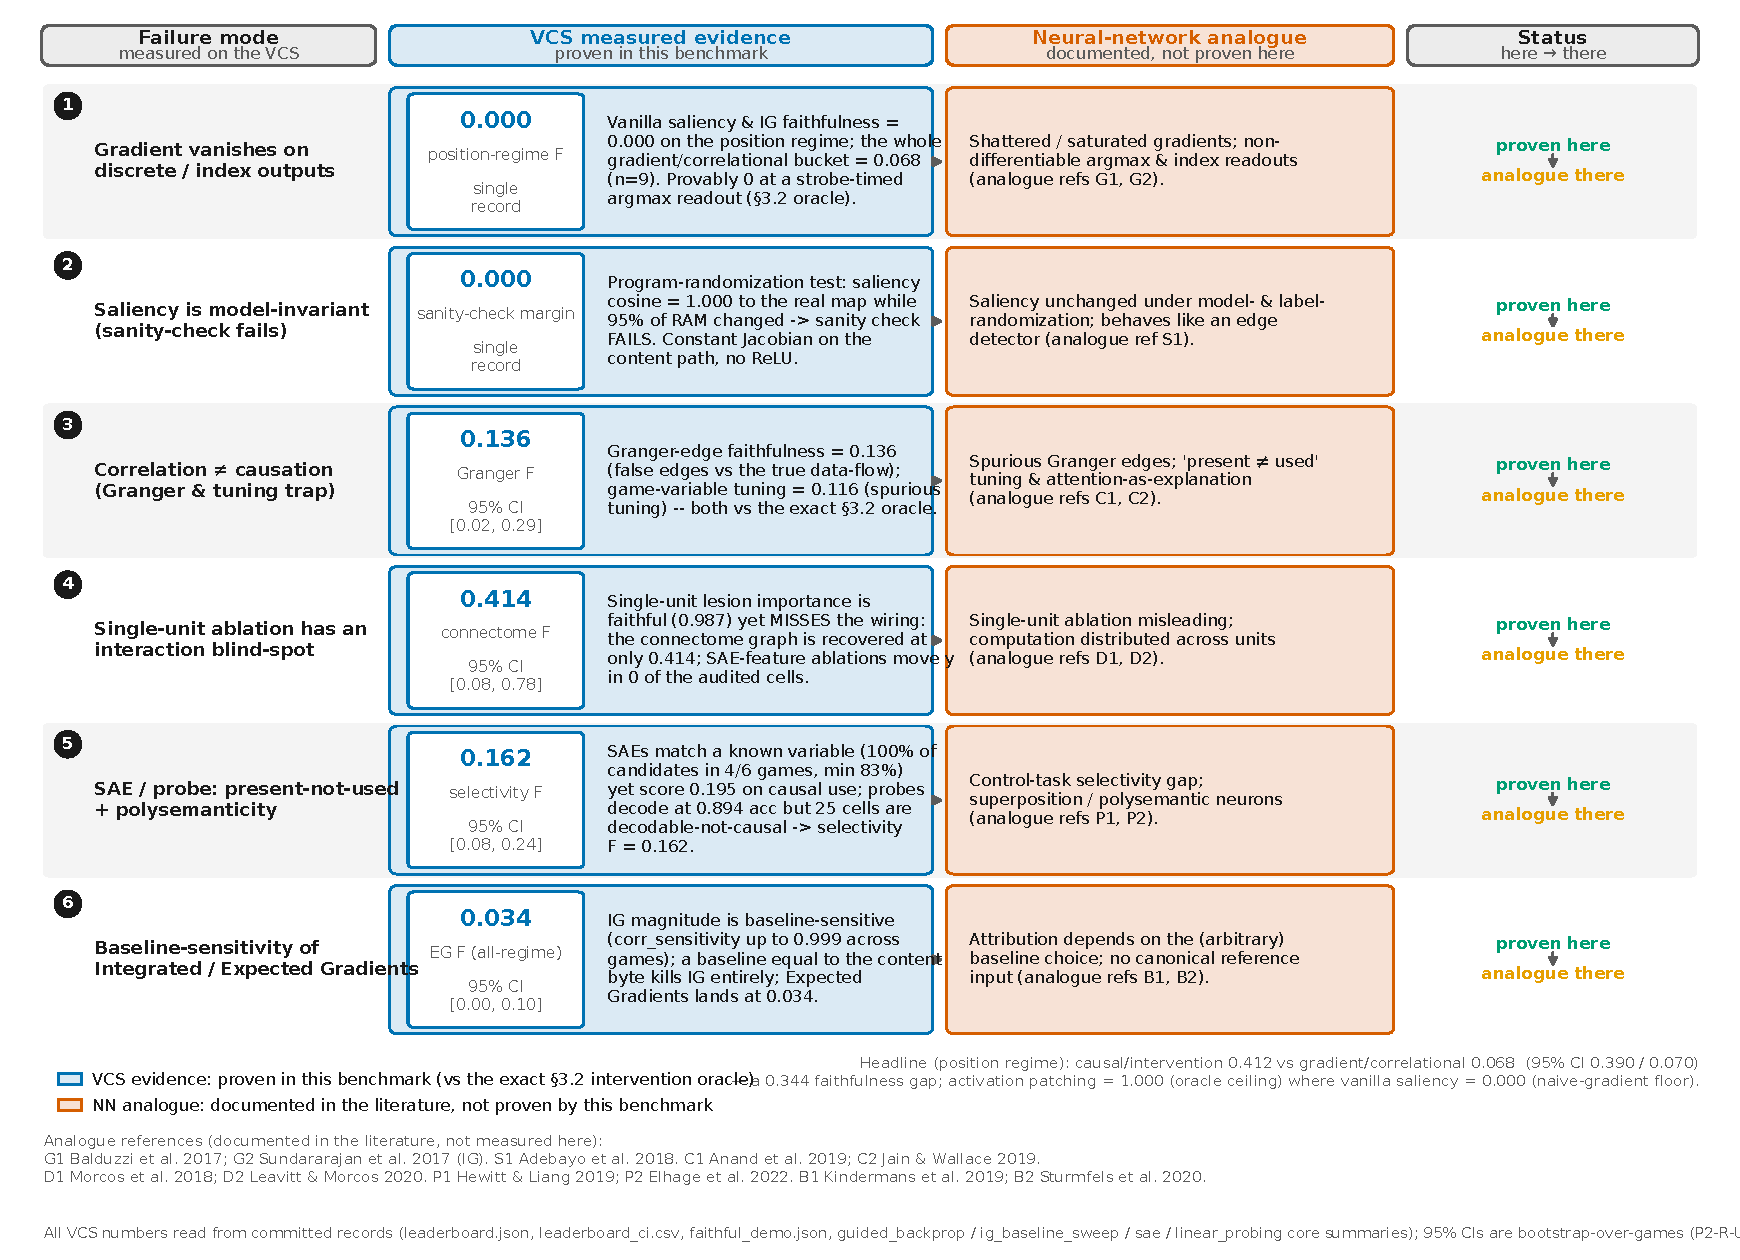
\includegraphics[width=\textwidth]{../figures/fig5_representativeness_map_full.pdf}
\caption{\textbf{Full VCS-to-NN representativeness map.} The full-density version of the
main-text map (Fig.~\ref{fig:representativeness}): each VCS failure mode is placed against its documented
neural-network analogue from the literature. The neural-network column records documented
analogues, not parallels proven by this benchmark; the oracle is the intervention oracle of
\Sectionname3.2, and the underlying per-method values trace to
\texttt{compare/out/leaderboard.json} via Sec.~\ref{supp:provenance}. Note that this full
map is the figure the simplified main-text version condenses.}
\label{supp:fig:repmap}
\end{figure}

\begin{figure}[t]
\centering
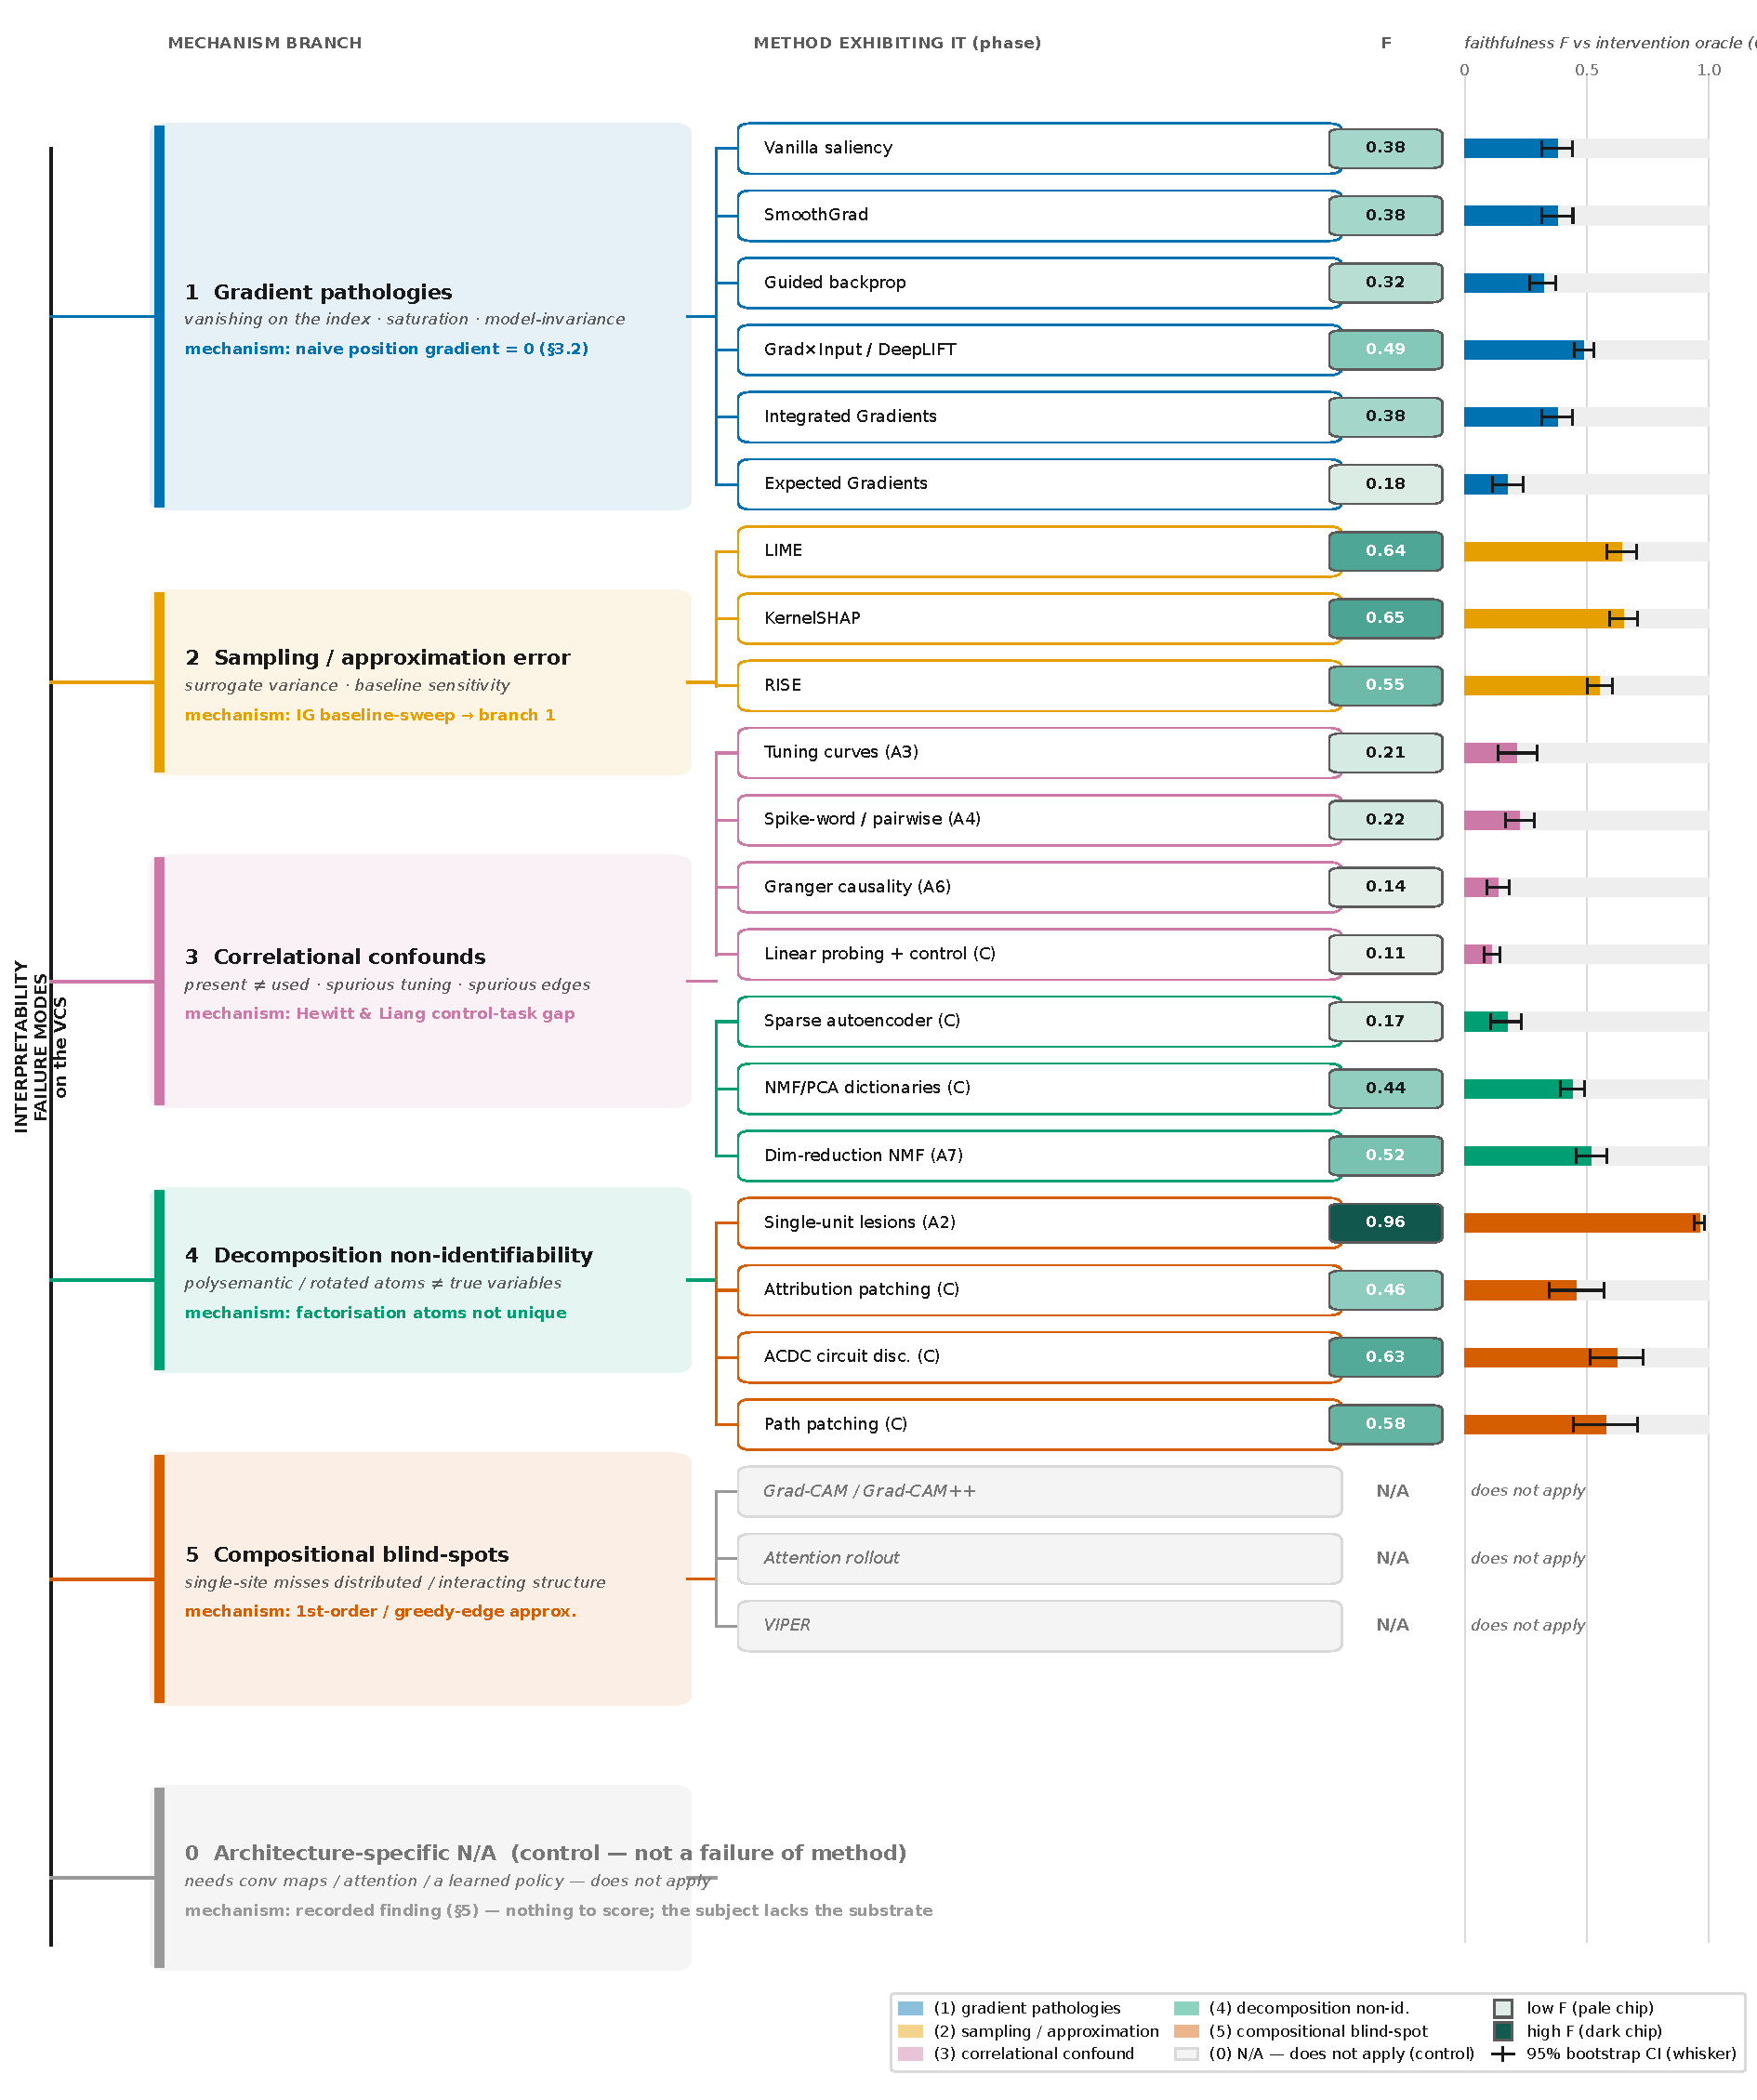
\includegraphics[width=\textwidth]{../figures/fig6_failure_taxonomy_full.pdf}
\caption{\textbf{Full failure taxonomy.} The full-density version of the main-text taxonomy
(Fig.~\ref{fig:taxonomy}): the families of interpretability failure observed on the machine, each annotated
with its faithfulness against the intervention oracle (\Sectionname3.2), reported as $F$ with its
$95\%$ bootstrap confidence interval. The leaf values trace to
\texttt{compare/out/leaderboard.json} and \texttt{leaderboard\_ci.csv} via
Sec.~\ref{supp:provenance}. Note that the gradient and correlational branches collapse on
the discrete position regime, where the naive gradient is provably zero (Prop.~\ref{prop:zero}).}
\label{supp:fig:taxonomy}
\end{figure}

\section{Plausibility-proxy rubric and its sensitivity}\label{supp:plausibility}

The plausibility axis of the leaderboard is a documented, tradition-level proxy, not a
human-subjects measurement. This section records how each value was assigned. It also shows
that the headline contrast does not depend on the particular numbers chosen. The Methods
(\Sectionname\ref{sec:triad}) name two reporting axes. Faithfulness is measured on the machine against the
intervention oracle of \Sectionname\ref{sec:oracle}. The plausibility proxy stands in for how convincing a
tradition's explanations are usually taken to be. We assign the proxy once per method
tradition, before any faithfulness score on our machine is computed, so it cannot be tuned to
the result. Its only job is to expose the danger zone of explanations that look convincing yet
are unfaithful. For that job it must be coarse, fixed in advance, and sourced rather than
precise.

The rubric assigns one proxy per tradition on a fixed five-step scale. It scores two
documented properties of each tradition's typical output and takes their average. The first
property is whether the explanation produces a dense, picture-like artifact that a reader sees
as an account of the computation. Heatmaps and saliency-style maps over the input are read as
convincing by construction. This is the perceptual-immediacy axis. The second property is
whether the field has historically treated the tradition's output as a self-evident
explanation rather than a hypothesis to be tested. This is the adoption-as-explanation axis. A
tradition that scores high on both, such as gradient saliency, receives a high proxy. A
tradition whose output is an austere intervention table or a circuit edge list, rarely
mistaken for a finished story, receives a low one. The scale is deliberately blunt,
$\{0.3,0.5,0.55,0.75,0.8,0.85,0.9\}$. A proxy meant to expose a danger zone gains nothing from
false precision, and a finer scale would invite over-reading. Every value in
Table~\ref{supp:tab:plausrubric} traces to the \jkey{plausibility_proxy} field of the
per-method rows in \texttt{compare/out/leaderboard.json}. The table only groups those rows by
tradition and records the rationale.

\begin{table}[t]
\centering
\caption{\textbf{Plausibility-proxy rubric.} The proxy assigned to each method tradition,
with the documented rationale. Values are the \jkey{plausibility_proxy} field of the
leaderboard rows (\texttt{compare/out/leaderboard.json}). They are tradition-level and fixed
before any faithfulness score is computed, so the proxy cannot be tuned to the measured
faithfulness. A higher value means an explanation that the field tends to find more
convincing, not one that is more faithful. The oracle (\Sectionname\ref{sec:oracle}) is the positive control and
is not a method under test.}
\label{supp:tab:plausrubric}
\begin{tabular}{@{}llp{6.4cm}@{}}
\toprule
Tradition & Proxy & Rationale (documented basis) \\
\midrule
gradient        & $0.90$ & Dense input-space heatmaps read as a visual account of the
                            decision; the most widely adopted XAI outputs, routinely shown
                            as if self-explanatory. \\
probing         & $0.85$ & A trained decoder that ``finds'' a concept reads as evidence the
                            concept is used; high adoption, though decodability is not
                            causal use. \\
correlational   & $0.80$ & Tuning curves and coupling spectra match the neuroscience idiom
                            of a convincing single-unit account. \\
dim.\ reduction & $0.75$ & Low-dimensional factors and dictionary atoms look like a clean
                            summary of the representation. \\
intervention    & $0.55$ & Occlusion and counterfactual outputs are quantitative tables, less
                            immediately picture-like, treated as tests rather than stories. \\
causal          & $0.50$ & Circuit edge lists and patching results are austere artifacts
                            rarely mistaken for a finished narrative. \\
descriptive     & $0.30$ & Whole-state recording is an explicit non-explanation: it withholds
                            nothing and reads as a dump, not an account. \\
\midrule
oracle (control)& $1.00$ & The \Sectionname\ref{sec:oracle} ground truth by construction; positive control, not a
                            method under test. \\
\bottomrule
\end{tabular}
\end{table}

The paper draws a contrast between this proxy and measured faithfulness. On the committed
records the two move in opposite directions. Across the thirty methods under test the Spearman
rank correlation between faithfulness and the proxy is $-0.36$, a negative association.
The traditions the field finds most convincing are, on this machine, among the least faithful.
Eight methods fall in the danger zone, defined here as a proxy of at least $0.70$ together
with a faithfulness below $0.40$. They include the correlational neuroscience methods, Expected
Gradients, guided backprop, linear probing, and the sparse autoencoder. The per-method extreme
makes the point sharply. Vanilla saliency has the highest proxy, $0.9$, yet scores faithfulness
$0.115$ on the position regime. Activation patching has a lower proxy, $0.5$, and scores $1.0$.
Here the less faithful method is the more plausible one. These figures are produced by
\texttt{tools/xai\_study/compare/plausibility\_sensitivity.py} from the leaderboard and
recorded in \texttt{compare/out/plausibility\_sensitivity.csv}.

A proxy fixed by a coarse rubric raises the question of whether the contrast is an artifact of
the particular numbers. The answer is that it is not. We perturb the proxy under four
deterministic schemes and recompute the relationship each time. The analysis uses fixed,
index-keyed offsets rather than random draws, so it re-derives bit-for-bit. The first scheme
adds a fixed per-method jitter of magnitude $\sigma\in\{0.05,0.1,0.2\}$, alternating in sign by
row. The second compresses every proxy toward the common mean by a fraction $\sigma$, which
preserves the rank order of traditions. The third uses the same index-keyed offsets at
$\sigma\in\{0.1,0.2\}$, large enough to swap neighbouring traditions' ranks. The fourth drops
one whole tradition at a time and recomputes on the remainder. Across all fourteen
perturbations the rank correlation between faithfulness and proxy stays negative. It ranges
from $-0.76$ to $-0.08$. The danger zone stays populated, with
between four and ten methods. The per-method anchor sign holds in every scheme where both
anchor methods are present, the more plausible saliency remaining the less faithful. Two runs
bound the range. The strongest is the leave-the-gradient-tradition-out run. It removes the most
plausible and least faithful block at once, and still leaves six danger-zone methods and a rank
correlation of $-0.76$. The weakest is the leave-the-causal-tradition-out run, where the
correlation falls to $-0.08$, close to zero; removing the faithful causal block flattens the
association, so the contrast is carried in part by that block. Table~\ref{supp:tab:plaussens}
reports the full sweep. The contrast keeps its sign under every alternative proxy assignment we
tried: plausibility and faithfulness are not the same axis, and high plausibility is no
guarantee of faithfulness.

\begin{table}[t]
\centering
\caption{\textbf{Proxy-sensitivity sweep.} The faithfulness-versus-proxy relationship under
each perturbation, from \texttt{compare/out/plausibility\_sensitivity.csv}. ``$\rho$'' is the
Spearman rank correlation between faithfulness and proxy over the methods present. ``danger''
is the count of high-proxy ($\geq0.70$), low-faithfulness ($<0.40$) methods. ``anchor'' is
$1$ when the more plausible saliency is the less faithful of the saliency/activation-patching
pair, and blank where a leave-one-out run removes an anchor. The baseline rubric is the first
row. Across every scheme the correlation stays negative and the danger zone stays populated.}
\label{supp:tab:plaussens}
\begin{tabular}{@{}llrrrc@{}}
\toprule
Scheme & Param & $n$ & $\rho$ & Danger & Anchor \\
\midrule
baseline                & ---           & 30 & $-0.36$ &  8 & 1 \\
additive jitter         & $\sigma=0.05$ & 30 & $-0.40$ &  8 & 1 \\
additive jitter         & $\sigma=0.10$ & 30 & $-0.41$ &  8 & 1 \\
additive jitter         & $\sigma=0.20$ & 30 & $-0.42$ & 10 & 1 \\
rank-preserving         & $\sigma=0.10$ & 30 & $-0.36$ &  8 & 1 \\
rank-preserving         & $\sigma=0.20$ & 30 & $-0.36$ &  8 & 1 \\
rank-jittering          & $\sigma=0.10$ & 30 & $-0.41$ &  8 & 1 \\
rank-jittering          & $\sigma=0.20$ & 30 & $-0.42$ & 10 & 1 \\
leave-out causal        & ---           & 24 & $-0.08$ &  8 & \\
leave-out correlational & ---           & 26 & $-0.40$ &  4 & 1 \\
leave-out descriptive   & ---           & 29 & $-0.29$ &  8 & 1 \\
leave-out dim.\ red.    & ---           & 27 & $-0.34$ &  7 & 1 \\
leave-out gradient      & ---           & 20 & $-0.76$ &  6 & \\
leave-out intervention  & ---           & 25 & $-0.34$ &  8 & 1 \\
leave-out probing       & ---           & 29 & $-0.36$ &  7 & 1 \\
\bottomrule
\end{tabular}
\end{table}

 into main.tex). It is also
%% a self-contained \input target: the six S-files below carry all SI content the main
%% paper promises (improvement_instructions P0#2, P0#4; P1#13, P1#14, P1#21; P3#35, P3#36).
%%
%% It re-uses, but does not re-derive, the §3 F/S/M definitions (S03 is authoritative)
%% and the canonical method count "30 interpretability methods + the oracle positive
%% control = 31 rows" (S07 is authoritative). Every reported number traces to a committed
%% record under tools/xai_study/compare/out/ (verifiable via the §6.5 traceability table
%% of REPRODUCIBILITY.md and re-derived by S5 below).
%%
%% Standalone compile (for review, before R6 wires it into main): wrap this file in the
%% sn-jnl preamble of a scratch driver (\documentclass[sn-nature,pdflatex]{sn-jnl} +
%% graphicx, booktabs, multirow, amsmath, longtable) and %% supplement.tex — Supplementary Information for Paper 2 (xai_2_interpretability).
%%
%% SCRUM note (P2-R-SUPP): this fragment is \input{} into the main paper by the SM
%% integration write (R6 wires %% supplement.tex — Supplementary Information for Paper 2 (xai_2_interpretability).
%%
%% SCRUM note (P2-R-SUPP): this fragment is \input{} into the main paper by the SM
%% integration write (R6 wires \input{supplement/supplement} into main.tex). It is also
%% a self-contained \input target: the six S-files below carry all SI content the main
%% paper promises (improvement_instructions P0#2, P0#4; P1#13, P1#14, P1#21; P3#35, P3#36).
%%
%% It re-uses, but does not re-derive, the §3 F/S/M definitions (S03 is authoritative)
%% and the canonical method count "30 interpretability methods + the oracle positive
%% control = 31 rows" (S07 is authoritative). Every reported number traces to a committed
%% record under tools/xai_study/compare/out/ (verifiable via the §6.5 traceability table
%% of REPRODUCIBILITY.md and re-derived by S5 below).
%%
%% Standalone compile (for review, before R6 wires it into main): wrap this file in the
%% sn-jnl preamble of a scratch driver (\documentclass[sn-nature,pdflatex]{sn-jnl} +
%% graphicx, booktabs, multirow, amsmath, longtable) and \input{supplement}; the tables
%% render without overfull boxes and the two SI figures resolve from ../figures/.

\clearpage
\appendix

%% Breakable monospaced JSON key: lets long under_scored keys wrap inside narrow table
%% columns. Used by S5 (number provenance). Defined here so the S-files stay self-contained.
\providecommand{\jkey}[1]{\texttt{\expandafter\jkeyaux#1\relax}}
\makeatletter
\def\jkeyaux#1{\ifx\relax#1\else
  \ifx_#1\discretionary{}{}{}\char`\_\else
    \ifx.#1\discretionary{}{}{}.\else#1\fi\fi
  \expandafter\jkeyaux\fi}
\makeatother

\section*{Supplementary Information}
\setcounter{table}{0}
\setcounter{figure}{0}
\renewcommand{\thetable}{S\arabic{table}}
\renewcommand{\thefigure}{S\arabic{figure}}
\renewcommand{\thesection}{S\arabic{section}}
\setcounter{section}{0}

This Supplementary Information records what the main paper summarizes. We give the
per-method protocols (\Sectionname\ref{supp:protocols}) and the leaderboard schema with its glossary
(\Sectionname\ref{supp:schema}). We give the coverage and applicability of every method across games
and output regimes (\Sectionname\ref{supp:coverage}). We map each headline claim to its evidence
(\Sectionname\ref{supp:claims}). We trace the provenance of every headline number down to the record
file and command that produced it (\Sectionname\ref{supp:provenance}). We state plainly what the
paper does not claim (\Sectionname\ref{supp:notclaimed}). We give the plausibility-proxy rubric and
its sensitivity analysis (\Sectionname\ref{supp:plausibility}). The main text shows simplified forms
of two diagnostic figures; we reproduce both here at full resolution
(Figs.~\ref{supp:fig:repmap} and~\ref{supp:fig:taxonomy}).
The correctness triad $\mathrm{F}\wedge\mathrm{S}\wedge\mathrm{M}$ used throughout is the
one defined in the main Methods (\Sectionname\ref{sec:triad}); we reference it here rather than restating it. The
benchmark scores 30 interpretability methods together with the intervention oracle (\Sectionname\ref{sec:oracle})
as a positive control, for 31 leaderboard rows in total.

\input{supplement/S1_per_method_protocols}
\input{supplement/S2_benchmark_schema}
\input{supplement/S3_coverage_applicability}
\input{supplement/S4_claims_evidence}
\input{supplement/S5_number_provenance}
\input{supplement/S6_not_claimed}
\input{supplement/S7_plausibility}
 into main.tex). It is also
%% a self-contained \input target: the six S-files below carry all SI content the main
%% paper promises (improvement_instructions P0#2, P0#4; P1#13, P1#14, P1#21; P3#35, P3#36).
%%
%% It re-uses, but does not re-derive, the §3 F/S/M definitions (S03 is authoritative)
%% and the canonical method count "30 interpretability methods + the oracle positive
%% control = 31 rows" (S07 is authoritative). Every reported number traces to a committed
%% record under tools/xai_study/compare/out/ (verifiable via the §6.5 traceability table
%% of REPRODUCIBILITY.md and re-derived by S5 below).
%%
%% Standalone compile (for review, before R6 wires it into main): wrap this file in the
%% sn-jnl preamble of a scratch driver (\documentclass[sn-nature,pdflatex]{sn-jnl} +
%% graphicx, booktabs, multirow, amsmath, longtable) and %% supplement.tex — Supplementary Information for Paper 2 (xai_2_interpretability).
%%
%% SCRUM note (P2-R-SUPP): this fragment is \input{} into the main paper by the SM
%% integration write (R6 wires \input{supplement/supplement} into main.tex). It is also
%% a self-contained \input target: the six S-files below carry all SI content the main
%% paper promises (improvement_instructions P0#2, P0#4; P1#13, P1#14, P1#21; P3#35, P3#36).
%%
%% It re-uses, but does not re-derive, the §3 F/S/M definitions (S03 is authoritative)
%% and the canonical method count "30 interpretability methods + the oracle positive
%% control = 31 rows" (S07 is authoritative). Every reported number traces to a committed
%% record under tools/xai_study/compare/out/ (verifiable via the §6.5 traceability table
%% of REPRODUCIBILITY.md and re-derived by S5 below).
%%
%% Standalone compile (for review, before R6 wires it into main): wrap this file in the
%% sn-jnl preamble of a scratch driver (\documentclass[sn-nature,pdflatex]{sn-jnl} +
%% graphicx, booktabs, multirow, amsmath, longtable) and \input{supplement}; the tables
%% render without overfull boxes and the two SI figures resolve from ../figures/.

\clearpage
\appendix

%% Breakable monospaced JSON key: lets long under_scored keys wrap inside narrow table
%% columns. Used by S5 (number provenance). Defined here so the S-files stay self-contained.
\providecommand{\jkey}[1]{\texttt{\expandafter\jkeyaux#1\relax}}
\makeatletter
\def\jkeyaux#1{\ifx\relax#1\else
  \ifx_#1\discretionary{}{}{}\char`\_\else
    \ifx.#1\discretionary{}{}{}.\else#1\fi\fi
  \expandafter\jkeyaux\fi}
\makeatother

\section*{Supplementary Information}
\setcounter{table}{0}
\setcounter{figure}{0}
\renewcommand{\thetable}{S\arabic{table}}
\renewcommand{\thefigure}{S\arabic{figure}}
\renewcommand{\thesection}{S\arabic{section}}
\setcounter{section}{0}

This Supplementary Information records what the main paper summarizes. We give the
per-method protocols (\Sectionname\ref{supp:protocols}) and the leaderboard schema with its glossary
(\Sectionname\ref{supp:schema}). We give the coverage and applicability of every method across games
and output regimes (\Sectionname\ref{supp:coverage}). We map each headline claim to its evidence
(\Sectionname\ref{supp:claims}). We trace the provenance of every headline number down to the record
file and command that produced it (\Sectionname\ref{supp:provenance}). We state plainly what the
paper does not claim (\Sectionname\ref{supp:notclaimed}). We give the plausibility-proxy rubric and
its sensitivity analysis (\Sectionname\ref{supp:plausibility}). The main text shows simplified forms
of two diagnostic figures; we reproduce both here at full resolution
(Figs.~\ref{supp:fig:repmap} and~\ref{supp:fig:taxonomy}).
The correctness triad $\mathrm{F}\wedge\mathrm{S}\wedge\mathrm{M}$ used throughout is the
one defined in the main Methods (\Sectionname\ref{sec:triad}); we reference it here rather than restating it. The
benchmark scores 30 interpretability methods together with the intervention oracle (\Sectionname\ref{sec:oracle})
as a positive control, for 31 leaderboard rows in total.

\input{supplement/S1_per_method_protocols}
\input{supplement/S2_benchmark_schema}
\input{supplement/S3_coverage_applicability}
\input{supplement/S4_claims_evidence}
\input{supplement/S5_number_provenance}
\input{supplement/S6_not_claimed}
\input{supplement/S7_plausibility}
; the tables
%% render without overfull boxes and the two SI figures resolve from ../figures/.

\clearpage
\appendix

%% Breakable monospaced JSON key: lets long under_scored keys wrap inside narrow table
%% columns. Used by S5 (number provenance). Defined here so the S-files stay self-contained.
\providecommand{\jkey}[1]{\texttt{\expandafter\jkeyaux#1\relax}}
\makeatletter
\def\jkeyaux#1{\ifx\relax#1\else
  \ifx_#1\discretionary{}{}{}\char`\_\else
    \ifx.#1\discretionary{}{}{}.\else#1\fi\fi
  \expandafter\jkeyaux\fi}
\makeatother

\section*{Supplementary Information}
\setcounter{table}{0}
\setcounter{figure}{0}
\renewcommand{\thetable}{S\arabic{table}}
\renewcommand{\thefigure}{S\arabic{figure}}
\renewcommand{\thesection}{S\arabic{section}}
\setcounter{section}{0}

This Supplementary Information records what the main paper summarizes. We give the
per-method protocols (\Sectionname\ref{supp:protocols}) and the leaderboard schema with its glossary
(\Sectionname\ref{supp:schema}). We give the coverage and applicability of every method across games
and output regimes (\Sectionname\ref{supp:coverage}). We map each headline claim to its evidence
(\Sectionname\ref{supp:claims}). We trace the provenance of every headline number down to the record
file and command that produced it (\Sectionname\ref{supp:provenance}). We state plainly what the
paper does not claim (\Sectionname\ref{supp:notclaimed}). We give the plausibility-proxy rubric and
its sensitivity analysis (\Sectionname\ref{supp:plausibility}). The main text shows simplified forms
of two diagnostic figures; we reproduce both here at full resolution
(Figs.~\ref{supp:fig:repmap} and~\ref{supp:fig:taxonomy}).
The correctness triad $\mathrm{F}\wedge\mathrm{S}\wedge\mathrm{M}$ used throughout is the
one defined in the main Methods (\Sectionname\ref{sec:triad}); we reference it here rather than restating it. The
benchmark scores 30 interpretability methods together with the intervention oracle (\Sectionname\ref{sec:oracle})
as a positive control, for 31 leaderboard rows in total.

\section{Per-method protocols}\label{supp:protocols}

This section records five things for each method under test. It records the exact objects the
method consumes and produces, the reference it is scored against, its sampling or optimization
budget, the metric that turns its output into a faithfulness score, and the committed record
file (version-controlled, in the released repository) that holds the per-game results. All methods share one evaluation contract. We state that
contract once and then specialize it per method. Every method receives the same bit-exact VCS
state on each game of the scored set. We state the contract on the six core games
(\texttt{breakout}, \texttt{ms\_pacman}, \texttt{pong}, \texttt{qbert}, \texttt{seaquest},
\texttt{space\_invaders}), which carry the full tiered ground truth and the exact oracle and
serve as the running example; the aggregate leaderboard scores extend the identical protocol
to the 42-game scored set of \Sectionname\ref{supp:scoredset}. That state is not the boot screen.
It is a shared gameplay state, produced by a single seeded random-action stream (seed~$0$) run
for a $90$-frame prefix and then rolled forward for a $15$-frame analysis horizon. The stream is
deterministic, so every method sees the identical state on each game, and the run is asserted
bit-exact per game. An oracle cause-density gate screens the state before any method runs. The
gate counts how many candidate causes move the output above a floor and rejects states with too
few, so a near-flat oracle column cannot pass. This gate is what turns a degenerate frame into a
usable one; on \texttt{seaquest} it raises the count of live candidate causes from $2$ to $19$.
The candidate-cause set is the machine's own state. This set is the RAM bytes together with the
CPU registers and the TIA and RIOT registers exposed by the substrate. The output every method
attributes over is a shared screen-buffer region read at the end of the analysis horizon, not a
single hand-picked pixel. The reference is the intervention oracle of \Sectionname\ref{sec:oracle},
evaluated by exact re-runs of the emulator under $\mathrm{do}(u)$. A method that
cannot be applied to a given output regime is recorded as not-applicable rather than scored
as zero. An empty result is therefore never read as a wrong one. Faithfulness is the F
axis of the main-text triad (\Sectionname\ref{sec:triad}); we reference that definition and do not restate it.
Records live under \texttt{tools/xai\_study/<phase>/out/}; the aggregate they feed is
\texttt{tools/xai\_study/compare/out/leaderboard.json}.
Table~\ref{supp:leaderboard} consolidates the triad scores for all thirty methods and the
oracle positive control in one place; the per-method protocols follow.

\begin{table*}[t]
\centering
\caption{\textbf{Consolidated leaderboard: all methods, all triad axes.} One row per method
across the three phases, plus the intervention oracle as a positive control. $F$ is
faithfulness (Pearson correlation against the oracle, with the bootstrap-over-games 95\% CI in
brackets), $S$ is sufficiency, $M$ is minimality, all as defined in \Sectionname\ref{sec:triad};
Plaus is the elicited plausibility prior and $n$ is the number of scored games. Attribution
methods that emit only a saliency have no defined $S$ or $M$ and are marked ``---''; A5
(field potentials) and A7 (dimensionality reduction) likewise lack the $S$/$M$ decomposition.
Values are transcribed from \texttt{tools/xai\_study/compare/out/leaderboard.json} (the
committed numbers of record).}
\label{supp:leaderboard}
\footnotesize
\setlength{\tabcolsep}{4pt}
\begin{tabularx}{\textwidth}{@{}Xccccccc@{}}
\toprule
Method & Phase & Tradition & $F$ (95\% CI) & $S$ & $M$ & Plaus & $n$ \\
\midrule
A1 connectomics & A & intervention & 0.207 [0.130, 0.293] & 0.971 & 0.967 & 0.55 & 35 \\
A2 lesions & A & intervention & 0.965 [0.942, 0.983] & 0.591 & 1.000 & 0.55 & 42 \\
A3 tuning curves & A & correlational & 0.213 [0.136, 0.295] & 0.200 & 0.928 & 0.80 & 42 \\
A4 spike-word / pairwise & A & correlational & 0.225 [0.166, 0.283] & 0.133 & 0.363 & 0.80 & 34 \\
A5 field potentials & A & correlational & 0.376 [0.323, 0.428] & --- & --- & 0.80 & 40 \\
A6 Granger & A & correlational & 0.136 [0.091, 0.184] & 0.884 & 0.647 & 0.80 & 35 \\
A7 dim.\ reduction & A & dim.\ red. & 0.519 [0.457, 0.581] & --- & --- & 0.75 & 42 \\
A8 whole-state & A & descriptive & 1.000 [1.000, 1.000] & 1.000 & 0.075 & 0.30 & 42 \\
\midrule
Vanilla saliency & B & gradient & 0.380 [0.316, 0.445] & --- & --- & 0.90 & 42 \\
smoothgrad & B & gradient & 0.380 [0.317, 0.445] & --- & --- & 0.90 & 42 \\
Guided backprop & B & gradient & 0.322 [0.267, 0.375] & --- & --- & 0.90 & 42 \\
Grad$\times$Input / DeepLIFT & B & gradient & 0.486 [0.448, 0.526] & --- & --- & 0.90 & 42 \\
Integrated Gradients & B & gradient & 0.379 [0.314, 0.444] & --- & --- & 0.90 & 42 \\
Expected Gradients & B & gradient & 0.175 [0.110, 0.240] & --- & --- & 0.90 & 42 \\
kernelshap & B & gradient & 0.652 [0.596, 0.709] & --- & --- & 0.90 & 42 \\
lime & B & gradient & 0.644 [0.582, 0.705] & --- & --- & 0.90 & 42 \\
rise & B & gradient & 0.552 [0.500, 0.600] & --- & --- & 0.90 & 42 \\
occlusion & B & intervention & 0.687 [0.624, 0.746] & --- & --- & 0.55 & 42 \\
Extremal perturbation & B & intervention & 0.461 [0.410, 0.513] & --- & --- & 0.55 & 42 \\
On-distribution counterfactual & B & intervention & 0.433 [0.343, 0.522] & --- & --- & 0.55 & 42 \\
\midrule
Activation patching & C & causal & 1.000 [1.000, 1.000] & --- & --- & 0.50 & 42 \\
Causal scrubbing & C & causal & 0.979 [0.940, 1.000] & 0.979 & 0.814 & 0.50 & 42 \\
Interchange interventions (DAS) & C & causal & 1.000 [1.000, 1.000] & --- & --- & 0.50 & 42 \\
Logit / tuned lens & C & causal & 0.820 [0.768, 0.871] & --- & 0.224 & 0.50 & 42 \\
Path patching & C & causal & 0.580 [0.452, 0.710] & --- & --- & 0.50 & 42 \\
ACDC & C & causal & 0.625 [0.514, 0.730] & 0.299 & 1.000 & 0.50 & 35 \\
Attribution patching & C & gradient & 0.456 [0.345, 0.573] & --- & --- & 0.90 & 42 \\
Linear probing (+ control) & C & probing & 0.240 [0.153, 0.346] & --- & 0.932 & 0.85 & 42 \\
NMF / PCA dictionaries & C & dim.\ red. & 0.102 [0.049, 0.160] & 0.751 & 0.966 & 0.75 & 42 \\
Sparse autoencoder & C & dim.\ red. & 0.153 [0.096, 0.218] & 0.183 & 0.934 & 0.75 & 40 \\
\midrule
Intervention oracle & --- & oracle & 1.000 [1.000, 1.000] & 1.000 & 1.000 & 1.00 & 1 \\
\bottomrule
\end{tabularx}
\end{table*}

The neuroscience analyses (Phase~A) treat the running machine as a brain. It asks how far
each classical analysis recovers the known mechanism on the shared gameplay state. Each
method's baseline is the exact data-flow graph or causal role that the substrate makes
available. Its budget is the scored set (\Sectionname\ref{supp:scoredset}) unless noted,
with the six-game core as the running example, and its scoring metric is named in
Table~\ref{supp:tab:phaseA}. One core cell is honestly degenerate. On \texttt{ms\_pacman} the
pairwise analysis (A4) finds no coupled candidate pair to score at that frame, so its
\texttt{ms\_pacman} value is uninformative rather than a failure; the other five games carry
it.

\begin{table}[t]
\centering
\caption{\textbf{Phase~A protocols (neuroscience analyses).} One row per method. The columns
give the input it reads, the reference it is scored against, the sampling or intervention
budget, the scoring metric, and the committed record. All eight run on the scored set
(\Sectionname\ref{supp:scoredset}), with the six core games as the running example;
faithfulness is the F axis of \Sectionname\ref{sec:triad}. The whole-state recording (A8) is included as a
descriptive upper bound on coverage. Its faithfulness $F$ is trivial, so we read it for its
minimality $M$.}
\label{supp:tab:phaseA}
\scriptsize
\setlength{\tabcolsep}{4pt}
\begin{tabular}{@{}p{1.7cm}p{2.6cm}p{1.9cm}p{2.6cm}p{1.0cm}@{}}
\toprule
Method & Input / candidate causes & Reference & Scoring metric & Record \\
\midrule
A1 connectomics & RAM/register activity over trajectory & data-flow graph & data-flow graph $F_1$ vs.\ oracle & A1 \\
A2 lesions & single-cell knockouts via $\mathrm{do}(u)$ & true causal role & lesion-importance $\rho$ vs.\ role & A2 \\
A3 tuning curves & per-cell response vs.\ variable & variable coupling & $1-$ spurious-tuning rate & A3 \\
A4 spike-word / pairwise & pairwise cell correlations & true coupling & corr.\ $\rho$ vs.\ coupling & A4 \\
A5 field potentials & pooled-activity spectra & true causal share & $1-$ clock-explained var. & A5 \\
A6 Granger & directed lag structure & true data-flow & $1-$ false-edge rate & A6 \\
A7 dim.\ reduction & NMF/PCA over activity & known variables & NMF matched-component frac. & A7 \\
A8 whole-state & full state record & oracle decomp. & minimality $M$ vs.\ oracle & A8 \\
\bottomrule
\end{tabular}

\smallskip
\noindent\scriptsize Records: \texttt{tools/xai\_study/phaseA\_kording/out/A\{1..8\}\_*}; all
eight run on the 42-game scored set (\Sectionname\ref{supp:scoredset}), with the six core
games as the running example (\jkey{n_games} per method in \jkey{leaderboard.json}).
\end{table}

The attribution methods (Phase~B) run the everyday XAI toolbox over the same gameplay state.
These methods produce a real-valued saliency or attribution over the candidate-cause set.
We score that output by Pearson correlation against the oracle attribution. The gradient family
runs with the bilinear sub-pixel sampler turned on, so it is scored on a real position gradient
and not on the naive one. The naive gradient of the discrete position output is provably zero
(Prop.~\ref{prop:zero}); the sampler restores a finite gradient, but the restored gradient is
low and mixed in faithfulness rather than a fix. Expected Gradients draws its reference pool
from the states of the same seeded gameplay trajectory, not from a synthetic baseline. Two cells
are honestly degenerate and recorded as such. The on-distribution counterfactual returns a zero
delta on \texttt{space\_invaders}, \texttt{ms\_pacman}, and \texttt{qbert}, where its perturbation
does not move the shared output at that frame; those cells are marked not-valid rather than
scored. Expected Gradients scores low on the content regime of every game except \texttt{pong},
because the causal byte it should land on is static there. The budgets that matter are the
Monte-Carlo or perturbation counts of the sampling estimators, recorded per method in
Table~\ref{supp:tab:phaseB}. The seed-dispersion of the stochastic members is carried in
\texttt{leaderboard\_ci.csv} (\texttt{seed\_sd}, \texttt{seed\_sd\_source}) and reproduced
in \Sectionname\ref{supp:provenance}.

\begin{table}[t]
\centering
\caption{\textbf{Phase~B protocols (attribution methods).} Each method emits a saliency over
the candidate-cause set. We score it by Pearson correlation against the oracle attribution
(\Sectionname\ref{sec:oracle}). The reference is shared and the budget is the scored set of
\Sectionname\ref{supp:scoredset} (six core games as the running example). The budget column records the
sampling or perturbation count that drives each estimator. The seed column flags which
methods carry an independent-seed dispersion in \texttt{leaderboard\_ci.csv}.}
\label{supp:tab:phaseB}
\scriptsize
\setlength{\tabcolsep}{4pt}
\begin{tabular}{@{}p{2.9cm}p{1.75cm}p{4.3cm}p{1.15cm}@{}}
\toprule
Method & Tradition & Budget / hyperparameters & Seed sd \\
\midrule
Vanilla saliency & gradient & single backward pass & --- \\
smoothgrad & gradient & noise-averaged gradient; $\sigma$-robustness committed & 0.0 \\
Guided backprop & gradient & single guided pass & --- \\
Grad$\times$Input / DeepLIFT & gradient & DeepLIFT reference-difference & --- \\
Integrated Gradients & gradient & path integral, baseline = zero state & --- \\
Expected Gradients & gradient & expectation over baselines (refits) & yes \\
kernelshap & gradient & Monte-Carlo coalition sampling ($\propto 1/\sqrt{N}$) & 0.017 \\
lime & gradient & local linear fit, perturbation refits & 0.029 \\
rise & gradient & random-mask Monte-Carlo ($\propto 1/\sqrt{N}$) & 0.051 \\
occlusion & intervention & exhaustive single-cell masking & --- \\
Extremal perturbation & intervention & optimized mask, area-constrained & --- \\
On-distribution counterfactual & intervention & on-manifold $\mathrm{do}(u)$ resampling & --- \\
\bottomrule
\end{tabular}

\smallskip
\noindent\scriptsize Records: \texttt{tools/xai\_study/phaseB\_attribution/out/}; all twelve run
on the 42-game scored set (\Sectionname\ref{supp:scoredset}), six core games as the running
example, and are scored by Pearson correlation against the oracle (\Sectionname\ref{sec:oracle}). Seed
sd is the independent-seed dispersion from \texttt{leaderboard\_ci.csv}.
\end{table}

The mechanistic methods (Phase~C) are built to recover circuits. Each is scored
against the true data-flow or the exact recovered-minus-exact deviation. The causal members
of this phase are the ones that reach the oracle ceiling. We list their exact scoring metric
so that the ceiling is not read as a tautology. Each member is scored against the substrate's
known routine, and not against another method. Two members (NMF/PCA dictionaries and the
sparse autoencoder) are dimensionality-reduction methods carried here for comparison. The
sparse autoencoder has two aggregations that differ, which we reconcile in
\Sectionname\ref{supp:provenance}.

\begin{table}[t]
\centering
\caption{\textbf{Phase~C protocols (mechanistic methods).} Each method is scored against the
substrate's known circuit or the exact recovered-minus-exact deviation (\Sectionname\ref{sec:oracle}), and not
against another method. This is what keeps the oracle ceiling non-circular. The probing and
dictionary-learning members are included for comparison with the causal members.}
\label{supp:tab:phaseC}
\scriptsize
\setlength{\tabcolsep}{4pt}
\begin{tabular}{@{}p{3.4cm}p{1.4cm}p{5.2cm}@{}}
\toprule
Method & Tradition & Scoring metric \\
\midrule
Activation patching & causal & $\max|\text{recovered}-\text{exact}|$ vs.\ oracle \\
Causal scrubbing & causal & scrubbing-preserved performance \\
Interchange interventions (DAS) & causal & aligned interchange accuracy \\
Logit / tuned lens & causal & logit-lens fidelity to true intermediate \\
Path patching & causal & path-circuit $F_1$ vs.\ true routine \\
ACDC & causal & discovered-circuit best $F_1$ vs.\ data-flow \\
Attribution patching & gradient & corr.\ of approximation vs.\ exact patch \\
Linear probing (+ control) & probing & selectivity vs.\ control task \\
NMF / PCA dictionaries & dim.\ red. & matched-component fraction vs.\ vars \\
Sparse autoencoder & dim.\ red. & feature-variable matched fraction \\
\bottomrule
\end{tabular}

\smallskip
\noindent\scriptsize Records: \texttt{tools/xai\_study/phaseC\_mechanistic/out/}; all ten run
on the 42-game scored set (\Sectionname\ref{supp:scoredset}), with the six core games as the
running example.
\end{table}

The intervention oracle is the positive control, not a method under test. It is the exact
$\mathrm{do}(u)$ ground truth of \Sectionname\ref{sec:oracle}, evaluated by re-running the bit-exact machine. It
attains $F=S=M=1.0$ by construction. Its record triple is the intervention oracle, the
content-path gradient oracle, and their cross-check
(\texttt{tools/xai\_study/ground\_truth/out/}). It anchors the ceiling against which every
other row is read, which is why it occupies the thirty-first leaderboard row.

\section{Benchmark schema and glossary}\label{supp:schema}

The leaderboard is built from a flat record schema. Stating it removes the ambiguity
about what a single number on the benchmark counts. Each method is run per game and writes a
per-game record under its phase's \texttt{out/} tree. The leaderboard aggregates those
records into one row per method by averaging over games. The schema columns of a leaderboard
row are given in Table~\ref{supp:tab:schema}. The aggregation rule is a mean over the
$n_{\text{games}}$ games. When a method emits several output records on one game, those records
are first reduced within that game. The faithfulness, sufficiency, and minimality columns
report the F, S, and M axes defined in \Sectionname\ref{sec:triad}. We do not re-derive those definitions here.

\begin{table}[t]
\centering
\caption{\textbf{Leaderboard row schema.} The columns of one row in
\texttt{compare/out/leaderboard.json} (\texttt{rows[\,]}) and its uncertainty companion
\texttt{leaderboard\_ci.csv}. The metric column names the per-method scoring function from
\Sectionname\ref{supp:protocols}; F, S, and M are the triad axes of \Sectionname\ref{sec:triad}. Aggregation is a mean
over $n_{\text{games}}$, with bootstrap confidence intervals over games (and, where present,
over records).}
\label{supp:tab:schema}
\footnotesize
\begin{tabular}{@{}p{3.0cm}p{8.4cm}@{}}
\toprule
Column & Meaning \\
\midrule
\texttt{phase} & phaseA\_kording, phaseB\_attribution, phaseC\_mechanistic, or ground\_truth \\
\texttt{method} & method identifier (the row key) \\
\texttt{tradition} & intervention, causal, gradient, correlational, \jkey{dim_reduction}, probing, descriptive, oracle \\
\jkey{n_games} & number of games the method was scored on (up to 42 for the scored set of \Sectionname\ref{supp:scoredset}; 1 for the oracle) \\
\jkey{n_records} & number of per-game output records aggregated into the row \\
\texttt{faithfulness} (F) & faithfulness vs.\ the intervention oracle (\Sectionname\ref{sec:oracle}), $[0,1]$, higher better \\
\jkey{faithfulness_ci95} & $95\%$ bootstrap CI half-width over games \\
\jkey{faithfulness_position_regime} & F restricted to the discrete sprite-position/index regime \\
\jkey{faithfulness_content_regime} & F restricted to the continuous content regime \\
\texttt{triad\_S} / \texttt{triad\_M} & sufficiency / minimality axes (\Sectionname\ref{sec:triad}), where applicable \\
\jkey{plausibility_proxy} & documented method-tradition proxy, $[0,1]$ --- not a human-subjects measurement \\
\jkey{is_positive_control} & 1 for the oracle row, 0 otherwise \\
\jkey{metric_names} & the per-method scoring function (\Sectionname\ref{supp:protocols}) \\
\texttt{commits} & the commit(s) at which the per-game records were produced \\
\bottomrule
\end{tabular}
\end{table}

We fix the vocabulary that the schema implies, because the review asked for a single
unambiguous method count. A \emph{method} is one interpretability technique, e.g.\
\texttt{vanilla\_saliency}. A \emph{method row} is its single aggregated line on the
leaderboard. A \emph{per-game record} is one method scored on one game, written under a phase
\texttt{out/} tree. An \emph{output record} is a per-game record for one output regime; a
method may emit several of these on one game. A \emph{family mean} is the average over the
members of a tradition family, e.g.\ causal/intervention. The \emph{oracle positive control}
is the exact $\mathrm{do}(u)$ ground truth of \Sectionname\ref{sec:oracle}, scored as a method to anchor the
ceiling. A \emph{not-applicable method} is one that does not apply to a given output regime;
it is recorded as N/A rather than as a zero. With this vocabulary the count is unambiguous.
The benchmark scores 30 interpretability methods together with the intervention
oracle as a positive control, for 31 leaderboard rows in total
(\texttt{leaderboard.json.n\_methods}~$=31$), aggregating 1773 per-game records over the
42-game scored set (\texttt{n\_per\_game\_records\_aggregated}~$=1773$): 8 methods in
Phase~A, 12 in Phase~B, 10 in Phase~C, and the one oracle row. This count is the canonical one
used in the abstract, the figures, and throughout this Supplement.

\section{Coverage and applicability}\label{supp:coverage}

The benchmark scores methods on a six-game core drawn from a larger bit-exact substrate. The
coverage table makes the scope of that choice explicit. Paper~1 validates the
differentiable VCS ports bit-for-bit against the \texttt{xitari} reference on all 64 Arcade
Learning Environment games, within a 30-frame RAM and 60-frame screen window. The
interpretability study reported here runs on the six games listed in
Table~\ref{supp:tab:coverage}. Every method is scored on a shared gameplay state, produced by
one seeded random-action stream (seed~$0$, $90$-frame prefix, $15$-frame analysis horizon), not
on the boot screen. This keeps the analysis inside the Paper~1 bit-exact window while giving the
oracle a rich, non-degenerate cause set to score against. We pick these six games because all
three tiers of ground truth (\Sectionname\ref{sec:tiers}) are available for them and the oracle is
exact. The remaining 58 games are
bit-exact substrate but are not scored here. Some fall outside the validated horizon for the
analyses we run. For others, the tiered labels they would need are not yet produced. They are
candidates for the larger sweep, and are not excluded for any methodological reason. The
horizon column records the validated window. The tier column records which of the three
ground-truth tiers (T1 exact intervention, T2 data-flow, T3 externally-supplied semantic
labels) is available.

\begin{table}[t]
\centering
\caption{\textbf{Core-game coverage.} The six core games carry exact tiered ground truth and
the full method battery. Faithfulness is scored within the Paper~1 bit-exact window. The
last two columns give the methods run and the per-game output records contributed. The wider
64-game substrate is bit-exact (Paper~1) but is reserved for the larger sweep. T3 labels are
external (\Sectionname\ref{sec:tiers}); we record this so the benchmark does not appear to certify them.}
\label{supp:tab:coverage}
\footnotesize
\setlength{\tabcolsep}{4pt}
\begin{tabular}{@{}p{2.4cm}p{1.9cm}p{1.5cm}p{1.7cm}p{1.5cm}p{1.4cm}@{}}
\toprule
Game & Paper-1 status & Horizon & Tiers & Methods run & Records \\
\midrule
breakout & bit-exact & 30/60 fr & T1,T2,T3 & 30 + oracle & per-game \\
ms\_pacman & bit-exact & 30/60 fr & T1,T2,T3 & 30 + oracle & per-game \\
pong & bit-exact & 30/60 fr & T1,T2,T3 & 30 + oracle & per-game \\
qbert & bit-exact & 30/60 fr & T1,T2,T3 & 30 + oracle & per-game \\
seaquest & bit-exact & 30/60 fr & T1,T2,T3 & 30 + oracle & per-game \\
space\_invaders & bit-exact & 30/60 fr & T1,T2,T3 & 30 + oracle & per-game \\
\midrule
58 further games & bit-exact (P1) & 30/60 fr & T1,T2 partial & reserved & --- \\
\bottomrule
\end{tabular}
\end{table}

A gameplay state can still be degenerate for a particular method, and the benchmark records
this rather than scoring it as a failure. The oracle cause-density gate is the first guard. It
counts how many candidate causes move the shared output above a floor, and rejects a state that
does not clear a minimum count, so a near-flat oracle column never reaches a method. On
\texttt{seaquest} the gate raises the count of live candidate causes at the analysis frame from
$2$ to $19$, which is what makes the game usable. Three residual degenerate cells survive the
gate and are marked, not scored as zero. On \texttt{ms\_pacman} the pairwise neuroscience
analysis (A4) finds no coupled candidate pair at that frame, so its cell is uninformative. The
on-distribution counterfactual returns a zero delta on \texttt{space\_invaders},
\texttt{ms\_pacman}, and \texttt{qbert}, where its perturbation does not move the shared output;
those cells are recorded as not-valid. Expected Gradients scores low on the content regime of
every game but \texttt{pong}, because the causal byte it should attribute to is static there.
None of these cells is read as a wrong answer.

Whether a method applies at all depends on what the method needs from its target. The
applicability matrix records that for every method family. The Phase~A neuroscience analyses
read the raw machine state and need neither a learned policy nor gradients. The Phase~B
attribution methods split into two groups. The gradient members need a differentiable forward
pass. The intervention members need only the ability to set state. The Phase~C mechanistic
methods need access to internal activations. The causal members among them also need the
ability to intervene. Table~\ref{supp:tab:applic} records, per family, whether the method
operates on the raw VCS, whether it requires a learned policy, gradients, internal layers or
attention, or external labels, whether it uses oracle-like interventions, and whether it
receives a supplied hypothesis. The table shows the same pattern the results confirm. The
families that score high on faithfulness are the ones that can intervene. The families that
collapse on the position regime are the gradient and correlational ones.

\begin{table}[t]
\centering
\caption{\textbf{Per-family applicability.} What each method family requires of its target.
``Intervenes'' marks oracle-like $\mathrm{do}(u)$ access; ``hypothesis'' marks methods that
receive a supplied circuit hypothesis to test. The raw-VCS column distinguishes analyses that
read machine state directly from those that need a differentiable or layered model. A blank
means the requirement does not apply.}
\label{supp:tab:applic}
\footnotesize
\begin{tabular}{@{}p{3.0cm}cccccc@{}}
\toprule
Family & raw VCS & policy & gradients & layers/attn & intervenes & hypothesis \\
\midrule
A neuroscience & yes & no & no & no & A2 only & no \\
B gradient & yes & no & yes & no & no & no \\
B intervention & yes & no & no & no & yes & no \\
C causal & yes & no & no & yes & yes & yes \\
C gradient (attr.\ patch) & yes & no & yes & yes & approx. & yes \\
C probing & yes & no & no & yes & no & no \\
C / A dim.\ reduction & yes & no & no & yes & no & no \\
oracle (control) & yes & no & no & yes & exact & --- \\
\bottomrule
\end{tabular}
\end{table}

\section{Claims and evidence}\label{supp:claims}

Every headline claim in the paper rests on a specific artifact. The table in this section
makes that dependency checkable. For each claim we list the figure or table that supports it,
the games and methods it uses, the metric, the artifact it traces to, and the limitation that
bounds it. Faithfulness, sufficiency, and minimality are the three axes of \Sectionname\ref{sec:triad}.
The numbers themselves are sourced in \Sectionname\ref{supp:provenance}. The table below names which
evidence supports which claim; it does not repeat the values. One split matters for how the
table is read. The all-regime faithfulness gap between causal/intervention and
gradient/correlational methods is $0.297$ with a $95\%$ interval of $[0.232,0.375]$ that
excludes zero, and it is the primary evidence for the headline. The position-only gap is
$0.238$ with an interval of $[-0.049,0.315]$ that crosses zero at six games. We report the
position gap as directional support, not as a significant result.

\begin{table}[t]
\centering
\caption{\textbf{Claims and their evidence.} Each headline claim maps to the figure or table
that supports it, the games and methods involved, the metric, the committed artifact, and the
limitation that bounds the claim. The artifact column points to the record that
\Sectionname\ref{supp:provenance} traces to a value. The limitation column states the scope, so the
claim is not read wider than the evidence.}
\label{supp:tab:claims}
\scriptsize
\setlength{\tabcolsep}{4pt}
\begin{tabular}{@{}p{3.0cm}p{1.9cm}p{1.8cm}p{1.9cm}p{2.4cm}@{}}
\toprule
Claim & Evidence & Methods / games & Metric & Limitation \\
\midrule
Causal/intervention methods beat gradient/correlational on faithfulness across all regimes & Fig.~\ref{fig:faithfulness}; leaderboard & 25 methods, 6 games & F mean (gap $0.297$) & robust: gap $0.297$ $[0.232,0.375]$ excludes zero; this all-regime gap is the primary evidence \\
The gap holds with the same sign on the discrete position regime & Fig.~\ref{fig:faithfulness}; \jkey{faithful_demo} & 13 rows, 6 games & F position (gap $0.238$) & directional only: gap $0.238$ $[-0.049,0.315]$ crosses zero at 6 games, so it is not significant \\
A faithful causal method reaches the oracle ceiling where the default tool stays low & \jkey{faithful_demo}; Fig.~\ref{fig:faithfulness} & act.\ patching vs.\ vanilla saliency, 6 games & F $1.0$ vs.\ $0.165$ (position regime; all-regimes saliency F $0.419$, plotted in Fig.~\ref{fig:faithfulness}) & one decisive pair \\
The naive gradient of a discrete position output is provably zero & Prop.~\ref{prop:zero} (\Sectionname\ref{sec:oracle}); \jkey{oracle_grad} & all gradient methods & grad@position $=0$; sampler restores $166$ & position path only; restored gradient is low/mixed \\
High plausibility coexists with low faithfulness (the danger zone) & Fig.~\ref{fig:faithfulness}; \jkey{faithful_demo} & vanilla saliency & proxy $0.9$, F $0.165$ (position regime; all-regimes F $0.419$, plotted in Fig.~\ref{fig:faithfulness}) & proxy, not measured plausibility \\
Faithful attribution recovers the wiring but not the computation's semantics & Fig.~\ref{fig:taxonomy} (\Sectionname\ref{supp:coverage}); discussion & Phase~B vs.\ C & F vs.\ S, M & necessary-condition stress test \\
The failure modes have documented NN analogues & Fig.~\ref{fig:representativeness} & taxonomy & --- & analogues, not proof \\
\bottomrule
\end{tabular}
\end{table}

\section{Number provenance}\label{supp:provenance}

Every headline number traces to a committed record, the script that produced it, and the
command that re-derives it. This section is the in-paper copy of that traceability table. It
mirrors \Sectionname6.5 of the reproducibility document
(\texttt{xai\_2\_interpretability/REPRODUCIBILITY.md}). The values are the measured, committed
ones at the current revision. The position-regime gap and its $95\%$ interval are read from
\texttt{tools/xai\_study/compare/out/position\_bootstrap.json}; the other aggregates from
\texttt{leaderboard.json}, rather than recomputed here. Each
record also carries \texttt{seed}, \texttt{where}, \texttt{commit}, and \texttt{timestamp}, so
the provenance of every value is self-documenting. The aggregate scores below are taken over
the 42-game scored battery of \Sectionname\ref{supp:scoredbattery}, not the six-game core;
each per-method row is a mean over the games on which that method applies (\jkey{n_games}
per method, e.g.\ 42 for most methods, 35 for ACDC and A1). The position-regime gap is now
significant on this battery.

\begin{table}[t]
\centering
\caption{\textbf{Headline-number provenance.} Each number $\rightarrow$ its committed record
and JSON key $\rightarrow$ the generating or aggregating script $\rightarrow$ the command
that reproduces it. Values are the measured, committed numbers at this revision (consistent
with REPRODUCIBILITY \Sectionname6.5); the position-regime gap CI is read from
\jkey{position_bootstrap.json}, all other aggregates from \jkey{leaderboard.json}. Paths are
relative to \texttt{tools/xai\_study/}.}
\label{supp:tab:provenance}
\scriptsize
\setlength{\tabcolsep}{3pt}
\renewcommand{\arraystretch}{1.15}
\begin{tabular}{@{}p{2.5cm}p{1.6cm}p{3.4cm}p{1.9cm}@{}}
\toprule
Number & Value & Record (JSON key) & Command \\
\midrule
Faithfulness gap, all regimes (causal $-$ gradient) & $0.3374$\newline {\scriptsize$[0.3103,0.3643]$, excl.\ $0$} & \jkey{position_bootstrap.json}: \jkey{all\_regime.family\_mean\_gap}, \jkey{ci95} & \jkey{position_bootstrap.py} \\
Causal/interv.\ mean F, all regimes & $0.7215$\newline {\scriptsize$n{=}11$} & \jkey{leaderboard.json}: \jkey{family_causal_intervention} \jkey{mean} & \jkey{leaderboard.py} \\
Gradient/corr.\ mean F, all regimes & $0.384$\newline {\scriptsize$n{=}14$} & \jkey{leaderboard.json}: \jkey{family_gradient_correlational} \jkey{mean} & \jkey{leaderboard.py} \\
Faithfulness gap, position regime (bootstrap over games) & $0.3268$\newline {\scriptsize$[0.1325,0.3702]$, excl.\ $0$} & \jkey{position_bootstrap.json}: \jkey{family_mean_gap}, \jkey{ci95} & \jkey{position_bootstrap.py} \\
Causal/interv.\ mean F, position regime & $0.561$\newline {\scriptsize$\pm0.3212$, $n{=}4$} & \jkey{leaderboard.json}: \jkey{family_..._intervention_position} \jkey{mean} & \jkey{leaderboard.py} \\
Gradient/corr.\ mean F, position regime & $0.2343$\newline {\scriptsize$\pm0.156$, $n{=}9$} & \jkey{leaderboard.json}: \jkey{family_..._correlational_position} \jkey{mean} & \jkey{leaderboard.py} \\
Decisive pair, position regime (act.\ patch vs.\ vanilla sal.) & $1.000$\newline vs.\ $0.115$ & \texttt{faithful\_demo}: \jkey{pair_contrast} & \jkey{faithful_demo.py} \\
Plausibility proxy, decisive pair & $0.5$ vs.\ $0.9$ & \texttt{faithful\_demo}: \jkey{...plausibility_proxy} & \jkey{faithful_demo.py} \\
ACDC sufficiency $S$ & $0.299$ & \jkey{leaderboard.json}: ACDC \jkey{triad_S} & \jkey{leaderboard.py} \\
Whole-state minimality $M$ & $0.0755$ & \jkey{leaderboard.json}: A8 \jkey{triad_M} & \jkey{leaderboard.py} \\
Methods scored (rows) & $31$ & \texttt{leaderboard}: \jkey{n_methods} & \jkey{leaderboard.py} \\
Per-game records aggregated & $1773$ & \texttt{leaderboard}: \jkey{n_per_game_records_aggregated} & \jkey{leaderboard.py} \\
Naive gradient, discrete position output & position $0$;\newline content $1.0$; sampler $166$ & \jkey{oracle_grad_pong.json}: \texttt{value}, \jkey{extra.sampler} & \jkey{oracle_grad.jl} \\
Exact oracle $\max|\Delta\text{score}|$ (Pong) & $17.0$ & \jkey{oracle_pong_score.json}: \texttt{value} & \jkey{oracle_intervene.jl} \\
\bottomrule
\end{tabular}

\smallskip
\noindent\scriptsize Scripts live under \texttt{tools/xai\_study/compare/} (Python) and
\texttt{tools/xai\_study/ground\_truth/} (Julia); records under the corresponding \texttt{out/}
trees. JSON keys are abbreviated with ``\texttt{...}'' where nested; the full paths are in
REPRODUCIBILITY \Sectionname6.5.
\end{table}

One number needs a reconciliation, and we record it rather than hide it. The sparse
autoencoder is the only method whose two aggregations disagree. On the 42-game scored battery
the over-games mean is $F=0.1526$ (\jkey{triad_F}) and the over-records mean is $0.1733$
(\jkey{faithfulness}); both are read from the sparse-autoencoder row of
\jkey{leaderboard.json}. The figures and the main-text leaderboard plot the over-records value
$0.1733$. We treat the over-games mean as the canonical row value for the aggregation rule of
\Sectionname\ref{supp:schema}, and report the over-records figure alongside it, so that text,
table, and figure agree on which aggregation each cites. No headline claim depends on which of
the two is read, since the sparse autoencoder sits near the floor under both.

\section{What this paper does not claim}\label{supp:notclaimed}

The benchmark is sharp precisely because its scope is narrow, and stating the boundaries
keeps the result from being read wider than the evidence carries it. We do not claim to
recover a program's semantics from scratch. The study measures whether an explanation names
the true causes and regenerates the behavior on a machine whose answer is already known; it
does not show that any method discovers the meaning of a routine without that ground truth in
hand, and the residual that faithfulness alone leaves behind, the gap between the wiring and
the computation, is the point rather than a result to be explained away.

We do not evaluate learned agents. The subject throughout is the bit-exact VCS itself, and
the candidate causes are its registers, RAM cells, and program variables, not the weights of
a trained policy. The neural-network parallels drawn in the discussion and in
Fig.~\ref{supp:fig:repmap} are documented analogues from the literature, not claims proven on
this benchmark; we label them as such so that a reader does not take a mapped failure mode
for a demonstrated one.

We do not prove that neural-network interpretability is impossible. The VCS gap is a
necessary-condition stress test: a method that fails to recover the wiring of a fully known
machine cannot be trusted to recover it on an unknown one, but a method that succeeds here is
not thereby certified on networks. The ``floor'' framing is an evidence-transfer argument,
not a proven lower bound on neural-network interpretability.

We do not measure human plausibility. The plausibility axis is a documented
method-tradition proxy, computed from a fixed rubric rather than collected from raters, and
we report it as a proxy throughout; its job is to expose the danger zone where a convincing
explanation is unfaithful, not to stand in for a human-subjects study. We also do not
redistribute the ROMs: the substrate is validated against an external reference, the records
are reproducible from committed artifacts without the ROMs, and the ROM provenance is given
as hashes so a third party supplies their own legally obtained copies.

\begin{figure}[t]
\centering
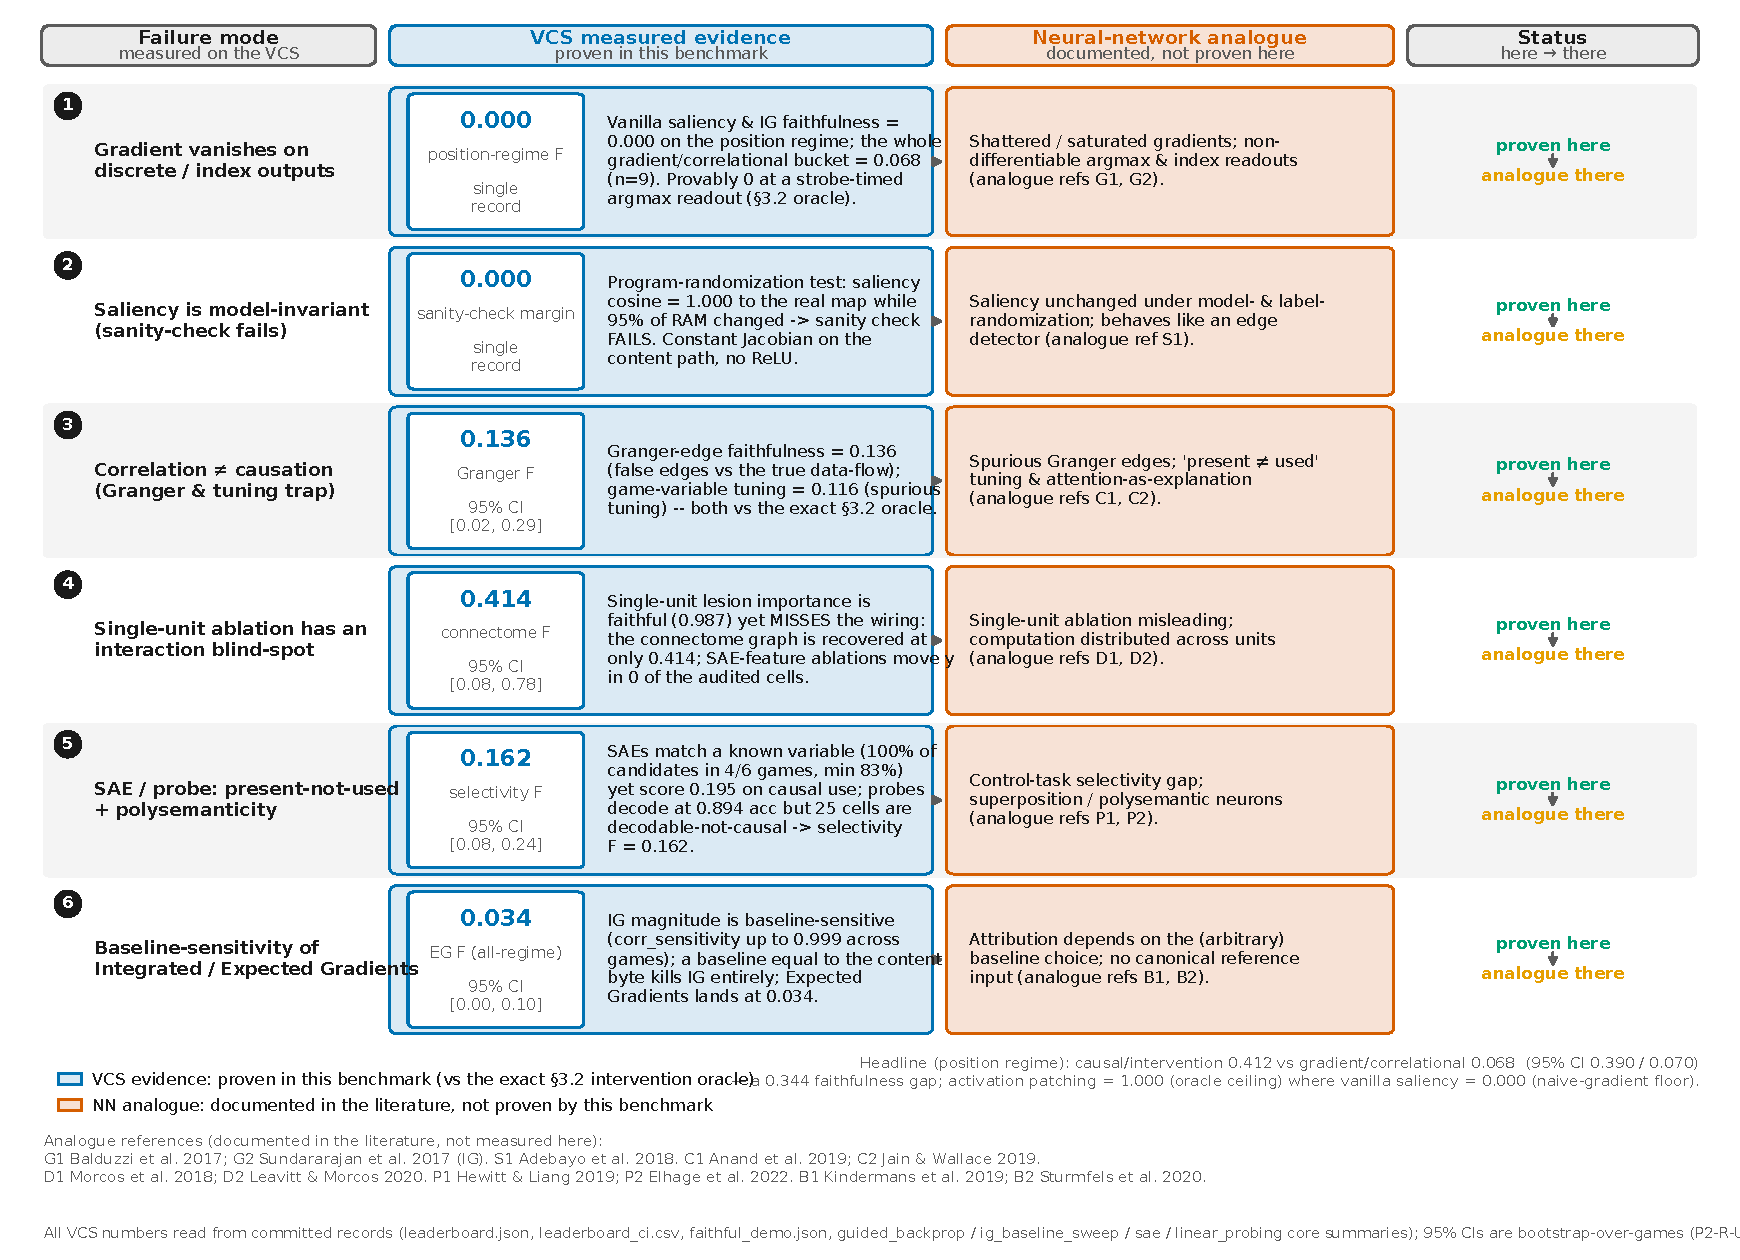
\includegraphics[width=\textwidth]{../figures/fig5_representativeness_map_full.pdf}
\caption{\textbf{Full VCS-to-NN representativeness map.} The full-density version of the
main-text map (Fig.~\ref{fig:representativeness}): each VCS failure mode is placed against its documented
neural-network analogue from the literature. The neural-network column records documented
analogues, not parallels proven by this benchmark; the oracle is the intervention oracle of
\Sectionname3.2, and the underlying per-method values trace to
\texttt{compare/out/leaderboard.json} via Sec.~\ref{supp:provenance}. Note that this full
map is the figure the simplified main-text version condenses.}
\label{supp:fig:repmap}
\end{figure}

\begin{figure}[t]
\centering
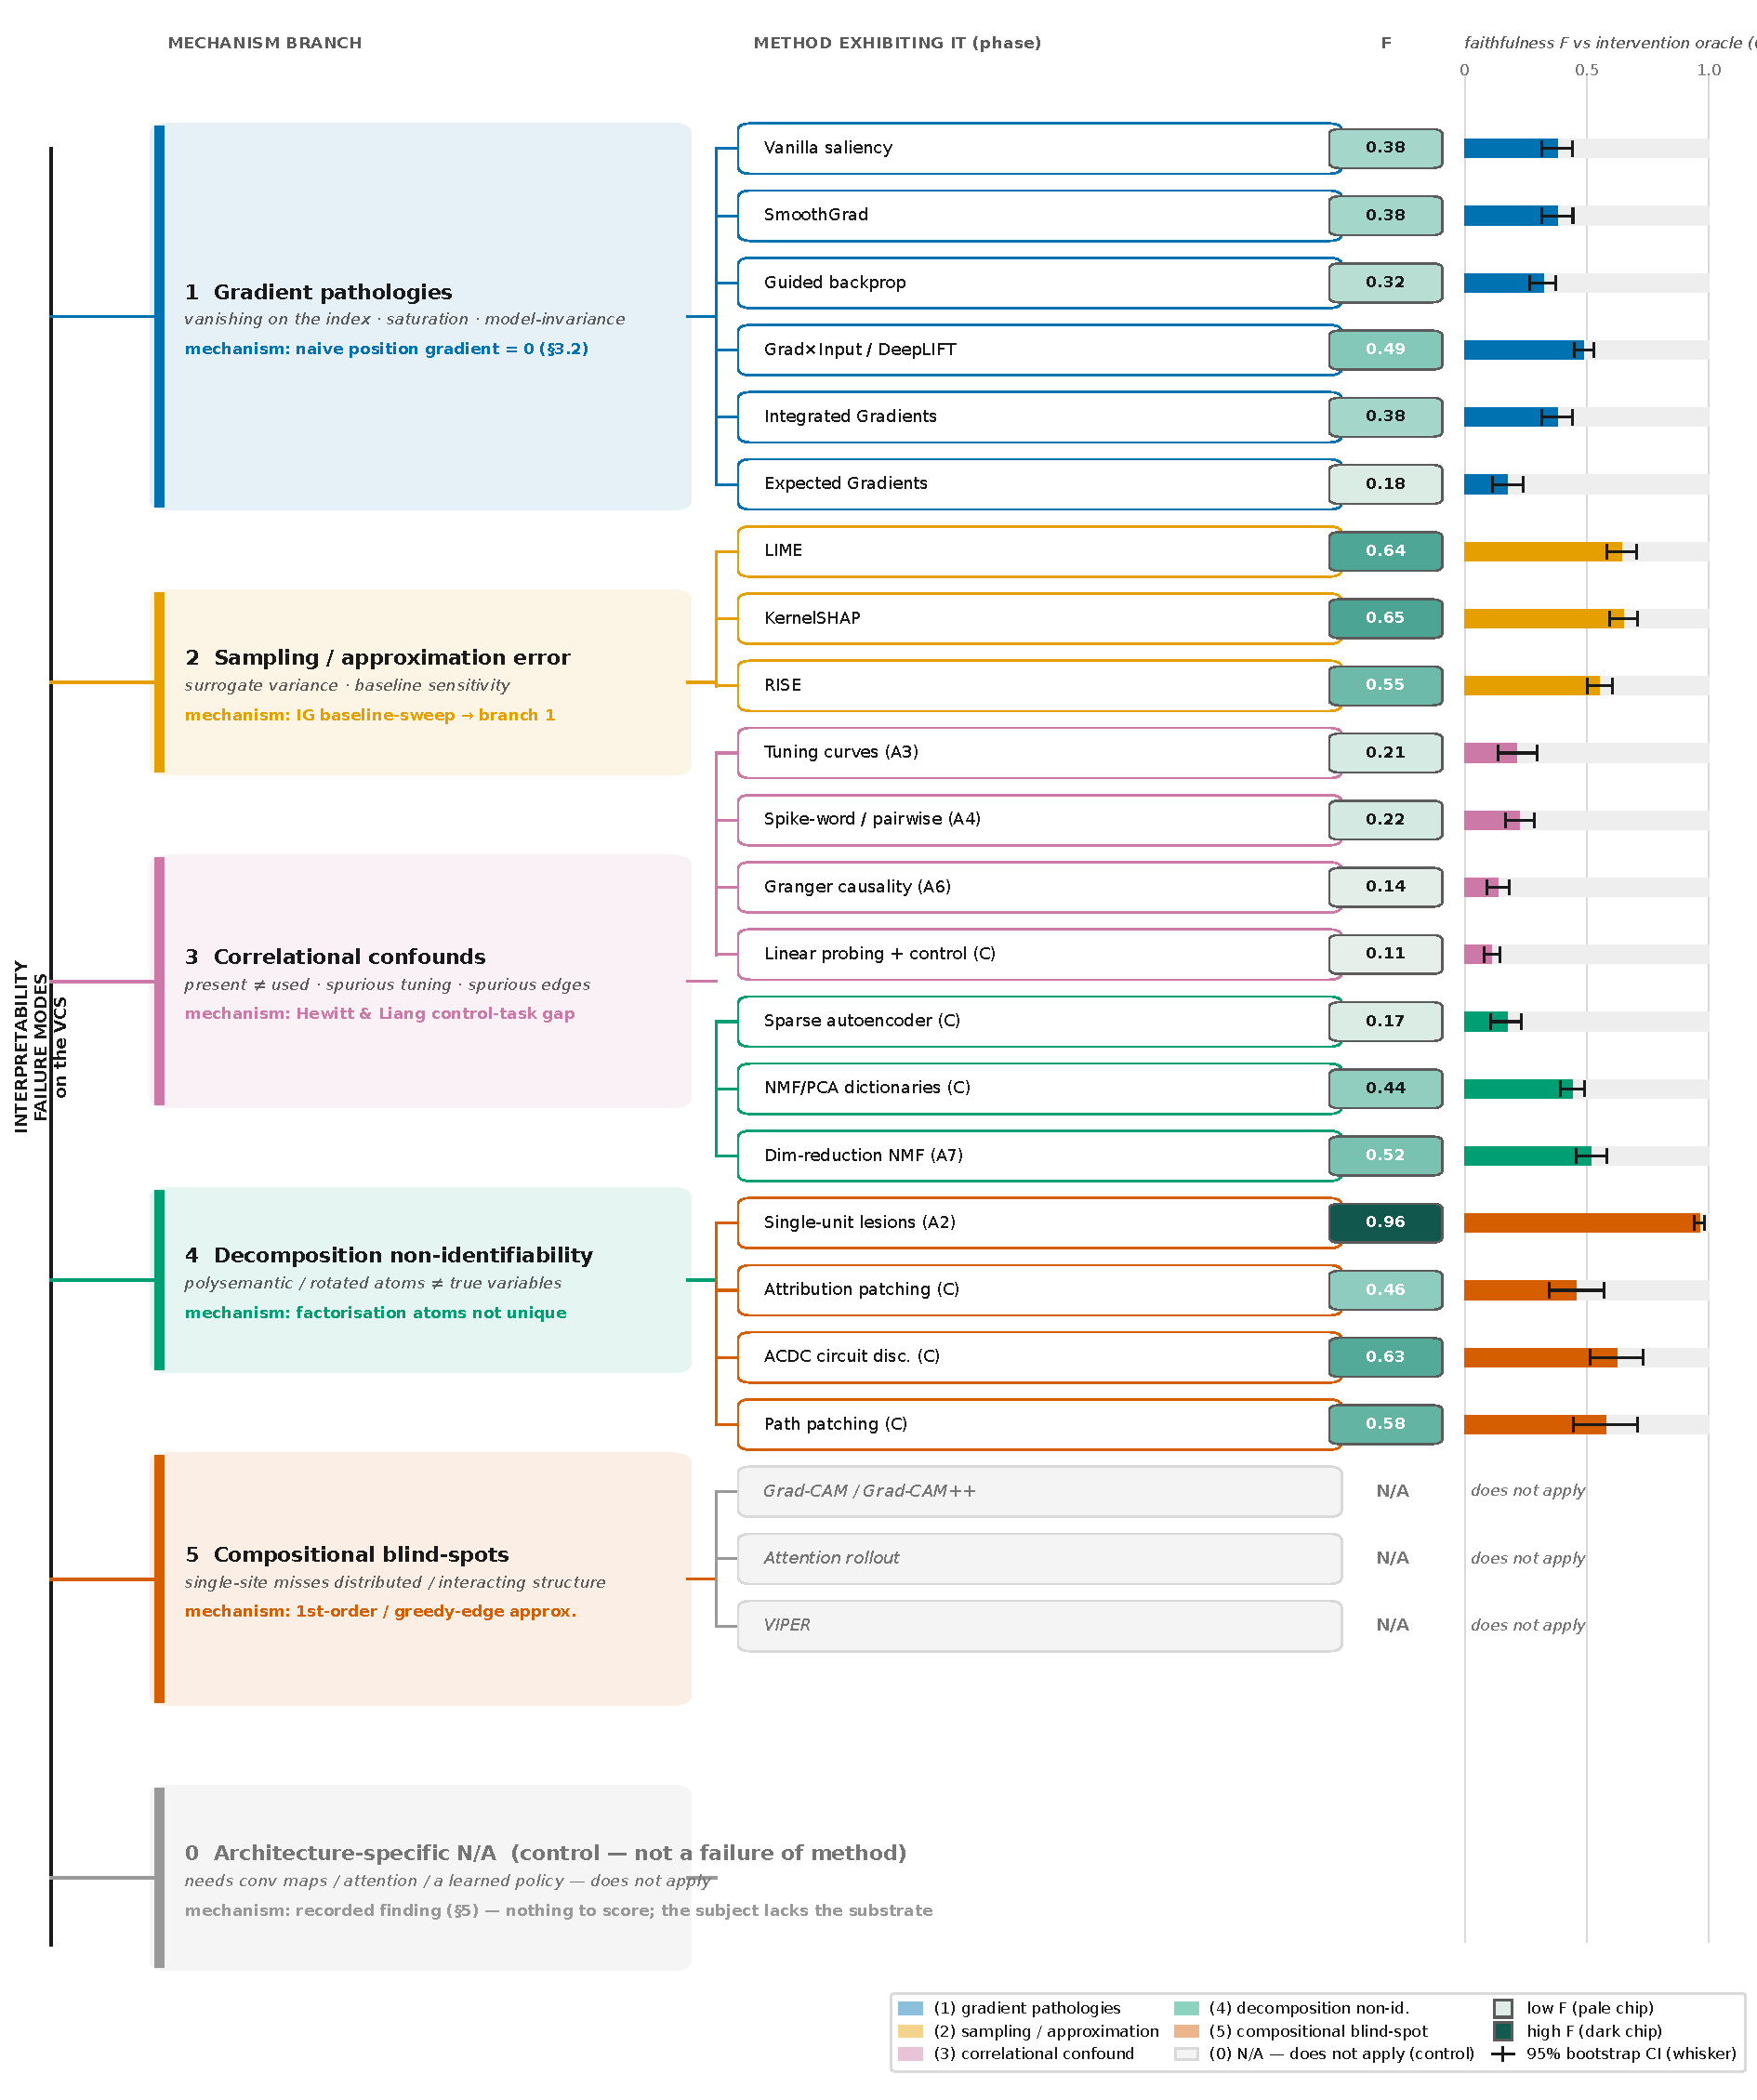
\includegraphics[width=\textwidth]{../figures/fig6_failure_taxonomy_full.pdf}
\caption{\textbf{Full failure taxonomy.} The full-density version of the main-text taxonomy
(Fig.~\ref{fig:taxonomy}): the families of interpretability failure observed on the machine, each annotated
with its faithfulness against the intervention oracle (\Sectionname3.2), reported as $F$ with its
$95\%$ bootstrap confidence interval. The leaf values trace to
\texttt{compare/out/leaderboard.json} and \texttt{leaderboard\_ci.csv} via
Sec.~\ref{supp:provenance}. Note that the gradient and correlational branches collapse on
the discrete position regime, where the naive gradient is provably zero (Prop.~\ref{prop:zero}).}
\label{supp:fig:taxonomy}
\end{figure}

\section{Plausibility-proxy rubric and its sensitivity}\label{supp:plausibility}

The plausibility axis of the leaderboard is a documented, tradition-level proxy, not a
human-subjects measurement. This section records how each value was assigned. It also shows
that the headline contrast does not depend on the particular numbers chosen. The Methods
(\Sectionname\ref{sec:triad}) name two reporting axes. Faithfulness is measured on the machine against the
intervention oracle of \Sectionname\ref{sec:oracle}. The plausibility proxy stands in for how convincing a
tradition's explanations are usually taken to be. We assign the proxy once per method
tradition, before any faithfulness score on our machine is computed, so it cannot be tuned to
the result. Its only job is to expose the danger zone of explanations that look convincing yet
are unfaithful. For that job it must be coarse, fixed in advance, and sourced rather than
precise.

The rubric assigns one proxy per tradition on a fixed five-step scale. It scores two
documented properties of each tradition's typical output and takes their average. The first
property is whether the explanation produces a dense, picture-like artifact that a reader sees
as an account of the computation. Heatmaps and saliency-style maps over the input are read as
convincing by construction. This is the perceptual-immediacy axis. The second property is
whether the field has historically treated the tradition's output as a self-evident
explanation rather than a hypothesis to be tested. This is the adoption-as-explanation axis. A
tradition that scores high on both, such as gradient saliency, receives a high proxy. A
tradition whose output is an austere intervention table or a circuit edge list, rarely
mistaken for a finished story, receives a low one. The scale is deliberately blunt,
$\{0.3,0.5,0.55,0.75,0.8,0.85,0.9\}$. A proxy meant to expose a danger zone gains nothing from
false precision, and a finer scale would invite over-reading. Every value in
Table~\ref{supp:tab:plausrubric} traces to the \jkey{plausibility_proxy} field of the
per-method rows in \texttt{compare/out/leaderboard.json}. The table only groups those rows by
tradition and records the rationale.

\begin{table}[t]
\centering
\caption{\textbf{Plausibility-proxy rubric.} The proxy assigned to each method tradition,
with the documented rationale. Values are the \jkey{plausibility_proxy} field of the
leaderboard rows (\texttt{compare/out/leaderboard.json}). They are tradition-level and fixed
before any faithfulness score is computed, so the proxy cannot be tuned to the measured
faithfulness. A higher value means an explanation that the field tends to find more
convincing, not one that is more faithful. The oracle (\Sectionname\ref{sec:oracle}) is the positive control and
is not a method under test.}
\label{supp:tab:plausrubric}
\begin{tabular}{@{}llp{6.4cm}@{}}
\toprule
Tradition & Proxy & Rationale (documented basis) \\
\midrule
gradient        & $0.90$ & Dense input-space heatmaps read as a visual account of the
                            decision; the most widely adopted XAI outputs, routinely shown
                            as if self-explanatory. \\
probing         & $0.85$ & A trained decoder that ``finds'' a concept reads as evidence the
                            concept is used; high adoption, though decodability is not
                            causal use. \\
correlational   & $0.80$ & Tuning curves and coupling spectra match the neuroscience idiom
                            of a convincing single-unit account. \\
dim.\ reduction & $0.75$ & Low-dimensional factors and dictionary atoms look like a clean
                            summary of the representation. \\
intervention    & $0.55$ & Occlusion and counterfactual outputs are quantitative tables, less
                            immediately picture-like, treated as tests rather than stories. \\
causal          & $0.50$ & Circuit edge lists and patching results are austere artifacts
                            rarely mistaken for a finished narrative. \\
descriptive     & $0.30$ & Whole-state recording is an explicit non-explanation: it withholds
                            nothing and reads as a dump, not an account. \\
\midrule
oracle (control)& $1.00$ & The \Sectionname\ref{sec:oracle} ground truth by construction; positive control, not a
                            method under test. \\
\bottomrule
\end{tabular}
\end{table}

The paper draws a contrast between this proxy and measured faithfulness. On the committed
records the two move in opposite directions. Across the thirty methods under test the Spearman
rank correlation between faithfulness and the proxy is $-0.36$, a negative association.
The traditions the field finds most convincing are, on this machine, among the least faithful.
Eight methods fall in the danger zone, defined here as a proxy of at least $0.70$ together
with a faithfulness below $0.40$. They include the correlational neuroscience methods, Expected
Gradients, guided backprop, linear probing, and the sparse autoencoder. The per-method extreme
makes the point sharply. Vanilla saliency has the highest proxy, $0.9$, yet scores faithfulness
$0.115$ on the position regime. Activation patching has a lower proxy, $0.5$, and scores $1.0$.
Here the less faithful method is the more plausible one. These figures are produced by
\texttt{tools/xai\_study/compare/plausibility\_sensitivity.py} from the leaderboard and
recorded in \texttt{compare/out/plausibility\_sensitivity.csv}.

A proxy fixed by a coarse rubric raises the question of whether the contrast is an artifact of
the particular numbers. The answer is that it is not. We perturb the proxy under four
deterministic schemes and recompute the relationship each time. The analysis uses fixed,
index-keyed offsets rather than random draws, so it re-derives bit-for-bit. The first scheme
adds a fixed per-method jitter of magnitude $\sigma\in\{0.05,0.1,0.2\}$, alternating in sign by
row. The second compresses every proxy toward the common mean by a fraction $\sigma$, which
preserves the rank order of traditions. The third uses the same index-keyed offsets at
$\sigma\in\{0.1,0.2\}$, large enough to swap neighbouring traditions' ranks. The fourth drops
one whole tradition at a time and recomputes on the remainder. Across all fourteen
perturbations the rank correlation between faithfulness and proxy stays negative. It ranges
from $-0.76$ to $-0.08$. The danger zone stays populated, with
between four and ten methods. The per-method anchor sign holds in every scheme where both
anchor methods are present, the more plausible saliency remaining the less faithful. Two runs
bound the range. The strongest is the leave-the-gradient-tradition-out run. It removes the most
plausible and least faithful block at once, and still leaves six danger-zone methods and a rank
correlation of $-0.76$. The weakest is the leave-the-causal-tradition-out run, where the
correlation falls to $-0.08$, close to zero; removing the faithful causal block flattens the
association, so the contrast is carried in part by that block. Table~\ref{supp:tab:plaussens}
reports the full sweep. The contrast keeps its sign under every alternative proxy assignment we
tried: plausibility and faithfulness are not the same axis, and high plausibility is no
guarantee of faithfulness.

\begin{table}[t]
\centering
\caption{\textbf{Proxy-sensitivity sweep.} The faithfulness-versus-proxy relationship under
each perturbation, from \texttt{compare/out/plausibility\_sensitivity.csv}. ``$\rho$'' is the
Spearman rank correlation between faithfulness and proxy over the methods present. ``danger''
is the count of high-proxy ($\geq0.70$), low-faithfulness ($<0.40$) methods. ``anchor'' is
$1$ when the more plausible saliency is the less faithful of the saliency/activation-patching
pair, and blank where a leave-one-out run removes an anchor. The baseline rubric is the first
row. Across every scheme the correlation stays negative and the danger zone stays populated.}
\label{supp:tab:plaussens}
\begin{tabular}{@{}llrrrc@{}}
\toprule
Scheme & Param & $n$ & $\rho$ & Danger & Anchor \\
\midrule
baseline                & ---           & 30 & $-0.36$ &  8 & 1 \\
additive jitter         & $\sigma=0.05$ & 30 & $-0.40$ &  8 & 1 \\
additive jitter         & $\sigma=0.10$ & 30 & $-0.41$ &  8 & 1 \\
additive jitter         & $\sigma=0.20$ & 30 & $-0.42$ & 10 & 1 \\
rank-preserving         & $\sigma=0.10$ & 30 & $-0.36$ &  8 & 1 \\
rank-preserving         & $\sigma=0.20$ & 30 & $-0.36$ &  8 & 1 \\
rank-jittering          & $\sigma=0.10$ & 30 & $-0.41$ &  8 & 1 \\
rank-jittering          & $\sigma=0.20$ & 30 & $-0.42$ & 10 & 1 \\
leave-out causal        & ---           & 24 & $-0.08$ &  8 & \\
leave-out correlational & ---           & 26 & $-0.40$ &  4 & 1 \\
leave-out descriptive   & ---           & 29 & $-0.29$ &  8 & 1 \\
leave-out dim.\ red.    & ---           & 27 & $-0.34$ &  7 & 1 \\
leave-out gradient      & ---           & 20 & $-0.76$ &  6 & \\
leave-out intervention  & ---           & 25 & $-0.34$ &  8 & 1 \\
leave-out probing       & ---           & 29 & $-0.36$ &  7 & 1 \\
\bottomrule
\end{tabular}
\end{table}

; the tables
%% render without overfull boxes and the two SI figures resolve from ../figures/.

\clearpage
\appendix

%% Breakable monospaced JSON key: lets long under_scored keys wrap inside narrow table
%% columns. Used by S5 (number provenance). Defined here so the S-files stay self-contained.
\providecommand{\jkey}[1]{\texttt{\expandafter\jkeyaux#1\relax}}
\makeatletter
\def\jkeyaux#1{\ifx\relax#1\else
  \ifx_#1\discretionary{}{}{}\char`\_\else
    \ifx.#1\discretionary{}{}{}.\else#1\fi\fi
  \expandafter\jkeyaux\fi}
\makeatother

\section*{Supplementary Information}
\setcounter{table}{0}
\setcounter{figure}{0}
\renewcommand{\thetable}{S\arabic{table}}
\renewcommand{\thefigure}{S\arabic{figure}}
\renewcommand{\thesection}{S\arabic{section}}
\setcounter{section}{0}

This Supplementary Information records what the main paper summarizes. We give the
per-method protocols (\Sectionname\ref{supp:protocols}) and the leaderboard schema with its glossary
(\Sectionname\ref{supp:schema}). We give the coverage and applicability of every method across games
and output regimes (\Sectionname\ref{supp:coverage}). We map each headline claim to its evidence
(\Sectionname\ref{supp:claims}). We trace the provenance of every headline number down to the record
file and command that produced it (\Sectionname\ref{supp:provenance}). We state plainly what the
paper does not claim (\Sectionname\ref{supp:notclaimed}). We give the plausibility-proxy rubric and
its sensitivity analysis (\Sectionname\ref{supp:plausibility}). The main text shows simplified forms
of two diagnostic figures; we reproduce both here at full resolution
(Figs.~\ref{supp:fig:repmap} and~\ref{supp:fig:taxonomy}).
The correctness triad $\mathrm{F}\wedge\mathrm{S}\wedge\mathrm{M}$ used throughout is the
one defined in the main Methods (\Sectionname\ref{sec:triad}); we reference it here rather than restating it. The
benchmark scores 30 interpretability methods together with the intervention oracle (\Sectionname\ref{sec:oracle})
as a positive control, for 31 leaderboard rows in total.

\section{Per-method protocols}\label{supp:protocols}

This section records five things for each method under test. It records the exact objects the
method consumes and produces, the reference it is scored against, its sampling or optimization
budget, the metric that turns its output into a faithfulness score, and the committed record
file (version-controlled, in the released repository) that holds the per-game results. All methods share one evaluation contract. We state that
contract once and then specialize it per method. Every method receives the same bit-exact VCS
state on each game of the scored set. We state the contract on the six core games
(\texttt{breakout}, \texttt{ms\_pacman}, \texttt{pong}, \texttt{qbert}, \texttt{seaquest},
\texttt{space\_invaders}), which carry the full tiered ground truth and the exact oracle and
serve as the running example; the aggregate leaderboard scores extend the identical protocol
to the 42-game scored set of \Sectionname\ref{supp:scoredset}. That state is not the boot screen.
It is a shared gameplay state, produced by a single seeded random-action stream (seed~$0$) run
for a $90$-frame prefix and then rolled forward for a $15$-frame analysis horizon. The stream is
deterministic, so every method sees the identical state on each game, and the run is asserted
bit-exact per game. An oracle cause-density gate screens the state before any method runs. The
gate counts how many candidate causes move the output above a floor and rejects states with too
few, so a near-flat oracle column cannot pass. This gate is what turns a degenerate frame into a
usable one; on \texttt{seaquest} it raises the count of live candidate causes from $2$ to $19$.
The candidate-cause set is the machine's own state. This set is the RAM bytes together with the
CPU registers and the TIA and RIOT registers exposed by the substrate. The output every method
attributes over is a shared screen-buffer region read at the end of the analysis horizon, not a
single hand-picked pixel. The reference is the intervention oracle of \Sectionname\ref{sec:oracle},
evaluated by exact re-runs of the emulator under $\mathrm{do}(u)$. A method that
cannot be applied to a given output regime is recorded as not-applicable rather than scored
as zero. An empty result is therefore never read as a wrong one. Faithfulness is the F
axis of the main-text triad (\Sectionname\ref{sec:triad}); we reference that definition and do not restate it.
Records live under \texttt{tools/xai\_study/<phase>/out/}; the aggregate they feed is
\texttt{tools/xai\_study/compare/out/leaderboard.json}.
Table~\ref{supp:leaderboard} consolidates the triad scores for all thirty methods and the
oracle positive control in one place; the per-method protocols follow.

\begin{table*}[t]
\centering
\caption{\textbf{Consolidated leaderboard: all methods, all triad axes.} One row per method
across the three phases, plus the intervention oracle as a positive control. $F$ is
faithfulness (Pearson correlation against the oracle, with the bootstrap-over-games 95\% CI in
brackets), $S$ is sufficiency, $M$ is minimality, all as defined in \Sectionname\ref{sec:triad};
Plaus is the elicited plausibility prior and $n$ is the number of scored games. Attribution
methods that emit only a saliency have no defined $S$ or $M$ and are marked ``---''; A5
(field potentials) and A7 (dimensionality reduction) likewise lack the $S$/$M$ decomposition.
Values are transcribed from \texttt{tools/xai\_study/compare/out/leaderboard.json} (the
committed numbers of record).}
\label{supp:leaderboard}
\footnotesize
\setlength{\tabcolsep}{4pt}
\begin{tabularx}{\textwidth}{@{}Xccccccc@{}}
\toprule
Method & Phase & Tradition & $F$ (95\% CI) & $S$ & $M$ & Plaus & $n$ \\
\midrule
A1 connectomics & A & intervention & 0.207 [0.130, 0.293] & 0.971 & 0.967 & 0.55 & 35 \\
A2 lesions & A & intervention & 0.965 [0.942, 0.983] & 0.591 & 1.000 & 0.55 & 42 \\
A3 tuning curves & A & correlational & 0.213 [0.136, 0.295] & 0.200 & 0.928 & 0.80 & 42 \\
A4 spike-word / pairwise & A & correlational & 0.225 [0.166, 0.283] & 0.133 & 0.363 & 0.80 & 34 \\
A5 field potentials & A & correlational & 0.376 [0.323, 0.428] & --- & --- & 0.80 & 40 \\
A6 Granger & A & correlational & 0.136 [0.091, 0.184] & 0.884 & 0.647 & 0.80 & 35 \\
A7 dim.\ reduction & A & dim.\ red. & 0.519 [0.457, 0.581] & --- & --- & 0.75 & 42 \\
A8 whole-state & A & descriptive & 1.000 [1.000, 1.000] & 1.000 & 0.075 & 0.30 & 42 \\
\midrule
Vanilla saliency & B & gradient & 0.380 [0.316, 0.445] & --- & --- & 0.90 & 42 \\
smoothgrad & B & gradient & 0.380 [0.317, 0.445] & --- & --- & 0.90 & 42 \\
Guided backprop & B & gradient & 0.322 [0.267, 0.375] & --- & --- & 0.90 & 42 \\
Grad$\times$Input / DeepLIFT & B & gradient & 0.486 [0.448, 0.526] & --- & --- & 0.90 & 42 \\
Integrated Gradients & B & gradient & 0.379 [0.314, 0.444] & --- & --- & 0.90 & 42 \\
Expected Gradients & B & gradient & 0.175 [0.110, 0.240] & --- & --- & 0.90 & 42 \\
kernelshap & B & gradient & 0.652 [0.596, 0.709] & --- & --- & 0.90 & 42 \\
lime & B & gradient & 0.644 [0.582, 0.705] & --- & --- & 0.90 & 42 \\
rise & B & gradient & 0.552 [0.500, 0.600] & --- & --- & 0.90 & 42 \\
occlusion & B & intervention & 0.687 [0.624, 0.746] & --- & --- & 0.55 & 42 \\
Extremal perturbation & B & intervention & 0.461 [0.410, 0.513] & --- & --- & 0.55 & 42 \\
On-distribution counterfactual & B & intervention & 0.433 [0.343, 0.522] & --- & --- & 0.55 & 42 \\
\midrule
Activation patching & C & causal & 1.000 [1.000, 1.000] & --- & --- & 0.50 & 42 \\
Causal scrubbing & C & causal & 0.979 [0.940, 1.000] & 0.979 & 0.814 & 0.50 & 42 \\
Interchange interventions (DAS) & C & causal & 1.000 [1.000, 1.000] & --- & --- & 0.50 & 42 \\
Logit / tuned lens & C & causal & 0.820 [0.768, 0.871] & --- & 0.224 & 0.50 & 42 \\
Path patching & C & causal & 0.580 [0.452, 0.710] & --- & --- & 0.50 & 42 \\
ACDC & C & causal & 0.625 [0.514, 0.730] & 0.299 & 1.000 & 0.50 & 35 \\
Attribution patching & C & gradient & 0.456 [0.345, 0.573] & --- & --- & 0.90 & 42 \\
Linear probing (+ control) & C & probing & 0.240 [0.153, 0.346] & --- & 0.932 & 0.85 & 42 \\
NMF / PCA dictionaries & C & dim.\ red. & 0.102 [0.049, 0.160] & 0.751 & 0.966 & 0.75 & 42 \\
Sparse autoencoder & C & dim.\ red. & 0.153 [0.096, 0.218] & 0.183 & 0.934 & 0.75 & 40 \\
\midrule
Intervention oracle & --- & oracle & 1.000 [1.000, 1.000] & 1.000 & 1.000 & 1.00 & 1 \\
\bottomrule
\end{tabularx}
\end{table*}

The neuroscience analyses (Phase~A) treat the running machine as a brain. It asks how far
each classical analysis recovers the known mechanism on the shared gameplay state. Each
method's baseline is the exact data-flow graph or causal role that the substrate makes
available. Its budget is the scored set (\Sectionname\ref{supp:scoredset}) unless noted,
with the six-game core as the running example, and its scoring metric is named in
Table~\ref{supp:tab:phaseA}. One core cell is honestly degenerate. On \texttt{ms\_pacman} the
pairwise analysis (A4) finds no coupled candidate pair to score at that frame, so its
\texttt{ms\_pacman} value is uninformative rather than a failure; the other five games carry
it.

\begin{table}[t]
\centering
\caption{\textbf{Phase~A protocols (neuroscience analyses).} One row per method. The columns
give the input it reads, the reference it is scored against, the sampling or intervention
budget, the scoring metric, and the committed record. All eight run on the scored set
(\Sectionname\ref{supp:scoredset}), with the six core games as the running example;
faithfulness is the F axis of \Sectionname\ref{sec:triad}. The whole-state recording (A8) is included as a
descriptive upper bound on coverage. Its faithfulness $F$ is trivial, so we read it for its
minimality $M$.}
\label{supp:tab:phaseA}
\scriptsize
\setlength{\tabcolsep}{4pt}
\begin{tabular}{@{}p{1.7cm}p{2.6cm}p{1.9cm}p{2.6cm}p{1.0cm}@{}}
\toprule
Method & Input / candidate causes & Reference & Scoring metric & Record \\
\midrule
A1 connectomics & RAM/register activity over trajectory & data-flow graph & data-flow graph $F_1$ vs.\ oracle & A1 \\
A2 lesions & single-cell knockouts via $\mathrm{do}(u)$ & true causal role & lesion-importance $\rho$ vs.\ role & A2 \\
A3 tuning curves & per-cell response vs.\ variable & variable coupling & $1-$ spurious-tuning rate & A3 \\
A4 spike-word / pairwise & pairwise cell correlations & true coupling & corr.\ $\rho$ vs.\ coupling & A4 \\
A5 field potentials & pooled-activity spectra & true causal share & $1-$ clock-explained var. & A5 \\
A6 Granger & directed lag structure & true data-flow & $1-$ false-edge rate & A6 \\
A7 dim.\ reduction & NMF/PCA over activity & known variables & NMF matched-component frac. & A7 \\
A8 whole-state & full state record & oracle decomp. & minimality $M$ vs.\ oracle & A8 \\
\bottomrule
\end{tabular}

\smallskip
\noindent\scriptsize Records: \texttt{tools/xai\_study/phaseA\_kording/out/A\{1..8\}\_*}; all
eight run on the 42-game scored set (\Sectionname\ref{supp:scoredset}), with the six core
games as the running example (\jkey{n_games} per method in \jkey{leaderboard.json}).
\end{table}

The attribution methods (Phase~B) run the everyday XAI toolbox over the same gameplay state.
These methods produce a real-valued saliency or attribution over the candidate-cause set.
We score that output by Pearson correlation against the oracle attribution. The gradient family
runs with the bilinear sub-pixel sampler turned on, so it is scored on a real position gradient
and not on the naive one. The naive gradient of the discrete position output is provably zero
(Prop.~\ref{prop:zero}); the sampler restores a finite gradient, but the restored gradient is
low and mixed in faithfulness rather than a fix. Expected Gradients draws its reference pool
from the states of the same seeded gameplay trajectory, not from a synthetic baseline. Two cells
are honestly degenerate and recorded as such. The on-distribution counterfactual returns a zero
delta on \texttt{space\_invaders}, \texttt{ms\_pacman}, and \texttt{qbert}, where its perturbation
does not move the shared output at that frame; those cells are marked not-valid rather than
scored. Expected Gradients scores low on the content regime of every game except \texttt{pong},
because the causal byte it should land on is static there. The budgets that matter are the
Monte-Carlo or perturbation counts of the sampling estimators, recorded per method in
Table~\ref{supp:tab:phaseB}. The seed-dispersion of the stochastic members is carried in
\texttt{leaderboard\_ci.csv} (\texttt{seed\_sd}, \texttt{seed\_sd\_source}) and reproduced
in \Sectionname\ref{supp:provenance}.

\begin{table}[t]
\centering
\caption{\textbf{Phase~B protocols (attribution methods).} Each method emits a saliency over
the candidate-cause set. We score it by Pearson correlation against the oracle attribution
(\Sectionname\ref{sec:oracle}). The reference is shared and the budget is the scored set of
\Sectionname\ref{supp:scoredset} (six core games as the running example). The budget column records the
sampling or perturbation count that drives each estimator. The seed column flags which
methods carry an independent-seed dispersion in \texttt{leaderboard\_ci.csv}.}
\label{supp:tab:phaseB}
\scriptsize
\setlength{\tabcolsep}{4pt}
\begin{tabular}{@{}p{2.9cm}p{1.75cm}p{4.3cm}p{1.15cm}@{}}
\toprule
Method & Tradition & Budget / hyperparameters & Seed sd \\
\midrule
Vanilla saliency & gradient & single backward pass & --- \\
smoothgrad & gradient & noise-averaged gradient; $\sigma$-robustness committed & 0.0 \\
Guided backprop & gradient & single guided pass & --- \\
Grad$\times$Input / DeepLIFT & gradient & DeepLIFT reference-difference & --- \\
Integrated Gradients & gradient & path integral, baseline = zero state & --- \\
Expected Gradients & gradient & expectation over baselines (refits) & yes \\
kernelshap & gradient & Monte-Carlo coalition sampling ($\propto 1/\sqrt{N}$) & 0.017 \\
lime & gradient & local linear fit, perturbation refits & 0.029 \\
rise & gradient & random-mask Monte-Carlo ($\propto 1/\sqrt{N}$) & 0.051 \\
occlusion & intervention & exhaustive single-cell masking & --- \\
Extremal perturbation & intervention & optimized mask, area-constrained & --- \\
On-distribution counterfactual & intervention & on-manifold $\mathrm{do}(u)$ resampling & --- \\
\bottomrule
\end{tabular}

\smallskip
\noindent\scriptsize Records: \texttt{tools/xai\_study/phaseB\_attribution/out/}; all twelve run
on the 42-game scored set (\Sectionname\ref{supp:scoredset}), six core games as the running
example, and are scored by Pearson correlation against the oracle (\Sectionname\ref{sec:oracle}). Seed
sd is the independent-seed dispersion from \texttt{leaderboard\_ci.csv}.
\end{table}

The mechanistic methods (Phase~C) are built to recover circuits. Each is scored
against the true data-flow or the exact recovered-minus-exact deviation. The causal members
of this phase are the ones that reach the oracle ceiling. We list their exact scoring metric
so that the ceiling is not read as a tautology. Each member is scored against the substrate's
known routine, and not against another method. Two members (NMF/PCA dictionaries and the
sparse autoencoder) are dimensionality-reduction methods carried here for comparison. The
sparse autoencoder has two aggregations that differ, which we reconcile in
\Sectionname\ref{supp:provenance}.

\begin{table}[t]
\centering
\caption{\textbf{Phase~C protocols (mechanistic methods).} Each method is scored against the
substrate's known circuit or the exact recovered-minus-exact deviation (\Sectionname\ref{sec:oracle}), and not
against another method. This is what keeps the oracle ceiling non-circular. The probing and
dictionary-learning members are included for comparison with the causal members.}
\label{supp:tab:phaseC}
\scriptsize
\setlength{\tabcolsep}{4pt}
\begin{tabular}{@{}p{3.4cm}p{1.4cm}p{5.2cm}@{}}
\toprule
Method & Tradition & Scoring metric \\
\midrule
Activation patching & causal & $\max|\text{recovered}-\text{exact}|$ vs.\ oracle \\
Causal scrubbing & causal & scrubbing-preserved performance \\
Interchange interventions (DAS) & causal & aligned interchange accuracy \\
Logit / tuned lens & causal & logit-lens fidelity to true intermediate \\
Path patching & causal & path-circuit $F_1$ vs.\ true routine \\
ACDC & causal & discovered-circuit best $F_1$ vs.\ data-flow \\
Attribution patching & gradient & corr.\ of approximation vs.\ exact patch \\
Linear probing (+ control) & probing & selectivity vs.\ control task \\
NMF / PCA dictionaries & dim.\ red. & matched-component fraction vs.\ vars \\
Sparse autoencoder & dim.\ red. & feature-variable matched fraction \\
\bottomrule
\end{tabular}

\smallskip
\noindent\scriptsize Records: \texttt{tools/xai\_study/phaseC\_mechanistic/out/}; all ten run
on the 42-game scored set (\Sectionname\ref{supp:scoredset}), with the six core games as the
running example.
\end{table}

The intervention oracle is the positive control, not a method under test. It is the exact
$\mathrm{do}(u)$ ground truth of \Sectionname\ref{sec:oracle}, evaluated by re-running the bit-exact machine. It
attains $F=S=M=1.0$ by construction. Its record triple is the intervention oracle, the
content-path gradient oracle, and their cross-check
(\texttt{tools/xai\_study/ground\_truth/out/}). It anchors the ceiling against which every
other row is read, which is why it occupies the thirty-first leaderboard row.

\section{Benchmark schema and glossary}\label{supp:schema}

The leaderboard is built from a flat record schema. Stating it removes the ambiguity
about what a single number on the benchmark counts. Each method is run per game and writes a
per-game record under its phase's \texttt{out/} tree. The leaderboard aggregates those
records into one row per method by averaging over games. The schema columns of a leaderboard
row are given in Table~\ref{supp:tab:schema}. The aggregation rule is a mean over the
$n_{\text{games}}$ games. When a method emits several output records on one game, those records
are first reduced within that game. The faithfulness, sufficiency, and minimality columns
report the F, S, and M axes defined in \Sectionname\ref{sec:triad}. We do not re-derive those definitions here.

\begin{table}[t]
\centering
\caption{\textbf{Leaderboard row schema.} The columns of one row in
\texttt{compare/out/leaderboard.json} (\texttt{rows[\,]}) and its uncertainty companion
\texttt{leaderboard\_ci.csv}. The metric column names the per-method scoring function from
\Sectionname\ref{supp:protocols}; F, S, and M are the triad axes of \Sectionname\ref{sec:triad}. Aggregation is a mean
over $n_{\text{games}}$, with bootstrap confidence intervals over games (and, where present,
over records).}
\label{supp:tab:schema}
\footnotesize
\begin{tabular}{@{}p{3.0cm}p{8.4cm}@{}}
\toprule
Column & Meaning \\
\midrule
\texttt{phase} & phaseA\_kording, phaseB\_attribution, phaseC\_mechanistic, or ground\_truth \\
\texttt{method} & method identifier (the row key) \\
\texttt{tradition} & intervention, causal, gradient, correlational, \jkey{dim_reduction}, probing, descriptive, oracle \\
\jkey{n_games} & number of games the method was scored on (up to 42 for the scored set of \Sectionname\ref{supp:scoredset}; 1 for the oracle) \\
\jkey{n_records} & number of per-game output records aggregated into the row \\
\texttt{faithfulness} (F) & faithfulness vs.\ the intervention oracle (\Sectionname\ref{sec:oracle}), $[0,1]$, higher better \\
\jkey{faithfulness_ci95} & $95\%$ bootstrap CI half-width over games \\
\jkey{faithfulness_position_regime} & F restricted to the discrete sprite-position/index regime \\
\jkey{faithfulness_content_regime} & F restricted to the continuous content regime \\
\texttt{triad\_S} / \texttt{triad\_M} & sufficiency / minimality axes (\Sectionname\ref{sec:triad}), where applicable \\
\jkey{plausibility_proxy} & documented method-tradition proxy, $[0,1]$ --- not a human-subjects measurement \\
\jkey{is_positive_control} & 1 for the oracle row, 0 otherwise \\
\jkey{metric_names} & the per-method scoring function (\Sectionname\ref{supp:protocols}) \\
\texttt{commits} & the commit(s) at which the per-game records were produced \\
\bottomrule
\end{tabular}
\end{table}

We fix the vocabulary that the schema implies, because the review asked for a single
unambiguous method count. A \emph{method} is one interpretability technique, e.g.\
\texttt{vanilla\_saliency}. A \emph{method row} is its single aggregated line on the
leaderboard. A \emph{per-game record} is one method scored on one game, written under a phase
\texttt{out/} tree. An \emph{output record} is a per-game record for one output regime; a
method may emit several of these on one game. A \emph{family mean} is the average over the
members of a tradition family, e.g.\ causal/intervention. The \emph{oracle positive control}
is the exact $\mathrm{do}(u)$ ground truth of \Sectionname\ref{sec:oracle}, scored as a method to anchor the
ceiling. A \emph{not-applicable method} is one that does not apply to a given output regime;
it is recorded as N/A rather than as a zero. With this vocabulary the count is unambiguous.
The benchmark scores 30 interpretability methods together with the intervention
oracle as a positive control, for 31 leaderboard rows in total
(\texttt{leaderboard.json.n\_methods}~$=31$), aggregating 1773 per-game records over the
42-game scored set (\texttt{n\_per\_game\_records\_aggregated}~$=1773$): 8 methods in
Phase~A, 12 in Phase~B, 10 in Phase~C, and the one oracle row. This count is the canonical one
used in the abstract, the figures, and throughout this Supplement.

\section{Coverage and applicability}\label{supp:coverage}

The benchmark scores methods on a six-game core drawn from a larger bit-exact substrate. The
coverage table makes the scope of that choice explicit. Paper~1 validates the
differentiable VCS ports bit-for-bit against the \texttt{xitari} reference on all 64 Arcade
Learning Environment games, within a 30-frame RAM and 60-frame screen window. The
interpretability study reported here runs on the six games listed in
Table~\ref{supp:tab:coverage}. Every method is scored on a shared gameplay state, produced by
one seeded random-action stream (seed~$0$, $90$-frame prefix, $15$-frame analysis horizon), not
on the boot screen. This keeps the analysis inside the Paper~1 bit-exact window while giving the
oracle a rich, non-degenerate cause set to score against. We pick these six games because all
three tiers of ground truth (\Sectionname\ref{sec:tiers}) are available for them and the oracle is
exact. The remaining 58 games are
bit-exact substrate but are not scored here. Some fall outside the validated horizon for the
analyses we run. For others, the tiered labels they would need are not yet produced. They are
candidates for the larger sweep, and are not excluded for any methodological reason. The
horizon column records the validated window. The tier column records which of the three
ground-truth tiers (T1 exact intervention, T2 data-flow, T3 externally-supplied semantic
labels) is available.

\begin{table}[t]
\centering
\caption{\textbf{Core-game coverage.} The six core games carry exact tiered ground truth and
the full method battery. Faithfulness is scored within the Paper~1 bit-exact window. The
last two columns give the methods run and the per-game output records contributed. The wider
64-game substrate is bit-exact (Paper~1) but is reserved for the larger sweep. T3 labels are
external (\Sectionname\ref{sec:tiers}); we record this so the benchmark does not appear to certify them.}
\label{supp:tab:coverage}
\footnotesize
\setlength{\tabcolsep}{4pt}
\begin{tabular}{@{}p{2.4cm}p{1.9cm}p{1.5cm}p{1.7cm}p{1.5cm}p{1.4cm}@{}}
\toprule
Game & Paper-1 status & Horizon & Tiers & Methods run & Records \\
\midrule
breakout & bit-exact & 30/60 fr & T1,T2,T3 & 30 + oracle & per-game \\
ms\_pacman & bit-exact & 30/60 fr & T1,T2,T3 & 30 + oracle & per-game \\
pong & bit-exact & 30/60 fr & T1,T2,T3 & 30 + oracle & per-game \\
qbert & bit-exact & 30/60 fr & T1,T2,T3 & 30 + oracle & per-game \\
seaquest & bit-exact & 30/60 fr & T1,T2,T3 & 30 + oracle & per-game \\
space\_invaders & bit-exact & 30/60 fr & T1,T2,T3 & 30 + oracle & per-game \\
\midrule
58 further games & bit-exact (P1) & 30/60 fr & T1,T2 partial & reserved & --- \\
\bottomrule
\end{tabular}
\end{table}

A gameplay state can still be degenerate for a particular method, and the benchmark records
this rather than scoring it as a failure. The oracle cause-density gate is the first guard. It
counts how many candidate causes move the shared output above a floor, and rejects a state that
does not clear a minimum count, so a near-flat oracle column never reaches a method. On
\texttt{seaquest} the gate raises the count of live candidate causes at the analysis frame from
$2$ to $19$, which is what makes the game usable. Three residual degenerate cells survive the
gate and are marked, not scored as zero. On \texttt{ms\_pacman} the pairwise neuroscience
analysis (A4) finds no coupled candidate pair at that frame, so its cell is uninformative. The
on-distribution counterfactual returns a zero delta on \texttt{space\_invaders},
\texttt{ms\_pacman}, and \texttt{qbert}, where its perturbation does not move the shared output;
those cells are recorded as not-valid. Expected Gradients scores low on the content regime of
every game but \texttt{pong}, because the causal byte it should attribute to is static there.
None of these cells is read as a wrong answer.

Whether a method applies at all depends on what the method needs from its target. The
applicability matrix records that for every method family. The Phase~A neuroscience analyses
read the raw machine state and need neither a learned policy nor gradients. The Phase~B
attribution methods split into two groups. The gradient members need a differentiable forward
pass. The intervention members need only the ability to set state. The Phase~C mechanistic
methods need access to internal activations. The causal members among them also need the
ability to intervene. Table~\ref{supp:tab:applic} records, per family, whether the method
operates on the raw VCS, whether it requires a learned policy, gradients, internal layers or
attention, or external labels, whether it uses oracle-like interventions, and whether it
receives a supplied hypothesis. The table shows the same pattern the results confirm. The
families that score high on faithfulness are the ones that can intervene. The families that
collapse on the position regime are the gradient and correlational ones.

\begin{table}[t]
\centering
\caption{\textbf{Per-family applicability.} What each method family requires of its target.
``Intervenes'' marks oracle-like $\mathrm{do}(u)$ access; ``hypothesis'' marks methods that
receive a supplied circuit hypothesis to test. The raw-VCS column distinguishes analyses that
read machine state directly from those that need a differentiable or layered model. A blank
means the requirement does not apply.}
\label{supp:tab:applic}
\footnotesize
\begin{tabular}{@{}p{3.0cm}cccccc@{}}
\toprule
Family & raw VCS & policy & gradients & layers/attn & intervenes & hypothesis \\
\midrule
A neuroscience & yes & no & no & no & A2 only & no \\
B gradient & yes & no & yes & no & no & no \\
B intervention & yes & no & no & no & yes & no \\
C causal & yes & no & no & yes & yes & yes \\
C gradient (attr.\ patch) & yes & no & yes & yes & approx. & yes \\
C probing & yes & no & no & yes & no & no \\
C / A dim.\ reduction & yes & no & no & yes & no & no \\
oracle (control) & yes & no & no & yes & exact & --- \\
\bottomrule
\end{tabular}
\end{table}

\section{Claims and evidence}\label{supp:claims}

Every headline claim in the paper rests on a specific artifact. The table in this section
makes that dependency checkable. For each claim we list the figure or table that supports it,
the games and methods it uses, the metric, the artifact it traces to, and the limitation that
bounds it. Faithfulness, sufficiency, and minimality are the three axes of \Sectionname\ref{sec:triad}.
The numbers themselves are sourced in \Sectionname\ref{supp:provenance}. The table below names which
evidence supports which claim; it does not repeat the values. One split matters for how the
table is read. The all-regime faithfulness gap between causal/intervention and
gradient/correlational methods is $0.297$ with a $95\%$ interval of $[0.232,0.375]$ that
excludes zero, and it is the primary evidence for the headline. The position-only gap is
$0.238$ with an interval of $[-0.049,0.315]$ that crosses zero at six games. We report the
position gap as directional support, not as a significant result.

\begin{table}[t]
\centering
\caption{\textbf{Claims and their evidence.} Each headline claim maps to the figure or table
that supports it, the games and methods involved, the metric, the committed artifact, and the
limitation that bounds the claim. The artifact column points to the record that
\Sectionname\ref{supp:provenance} traces to a value. The limitation column states the scope, so the
claim is not read wider than the evidence.}
\label{supp:tab:claims}
\scriptsize
\setlength{\tabcolsep}{4pt}
\begin{tabular}{@{}p{3.0cm}p{1.9cm}p{1.8cm}p{1.9cm}p{2.4cm}@{}}
\toprule
Claim & Evidence & Methods / games & Metric & Limitation \\
\midrule
Causal/intervention methods beat gradient/correlational on faithfulness across all regimes & Fig.~\ref{fig:faithfulness}; leaderboard & 25 methods, 6 games & F mean (gap $0.297$) & robust: gap $0.297$ $[0.232,0.375]$ excludes zero; this all-regime gap is the primary evidence \\
The gap holds with the same sign on the discrete position regime & Fig.~\ref{fig:faithfulness}; \jkey{faithful_demo} & 13 rows, 6 games & F position (gap $0.238$) & directional only: gap $0.238$ $[-0.049,0.315]$ crosses zero at 6 games, so it is not significant \\
A faithful causal method reaches the oracle ceiling where the default tool stays low & \jkey{faithful_demo}; Fig.~\ref{fig:faithfulness} & act.\ patching vs.\ vanilla saliency, 6 games & F $1.0$ vs.\ $0.165$ (position regime; all-regimes saliency F $0.419$, plotted in Fig.~\ref{fig:faithfulness}) & one decisive pair \\
The naive gradient of a discrete position output is provably zero & Prop.~\ref{prop:zero} (\Sectionname\ref{sec:oracle}); \jkey{oracle_grad} & all gradient methods & grad@position $=0$; sampler restores $166$ & position path only; restored gradient is low/mixed \\
High plausibility coexists with low faithfulness (the danger zone) & Fig.~\ref{fig:faithfulness}; \jkey{faithful_demo} & vanilla saliency & proxy $0.9$, F $0.165$ (position regime; all-regimes F $0.419$, plotted in Fig.~\ref{fig:faithfulness}) & proxy, not measured plausibility \\
Faithful attribution recovers the wiring but not the computation's semantics & Fig.~\ref{fig:taxonomy} (\Sectionname\ref{supp:coverage}); discussion & Phase~B vs.\ C & F vs.\ S, M & necessary-condition stress test \\
The failure modes have documented NN analogues & Fig.~\ref{fig:representativeness} & taxonomy & --- & analogues, not proof \\
\bottomrule
\end{tabular}
\end{table}

\section{Number provenance}\label{supp:provenance}

Every headline number traces to a committed record, the script that produced it, and the
command that re-derives it. This section is the in-paper copy of that traceability table. It
mirrors \Sectionname6.5 of the reproducibility document
(\texttt{xai\_2\_interpretability/REPRODUCIBILITY.md}). The values are the measured, committed
ones at the current revision. The position-regime gap and its $95\%$ interval are read from
\texttt{tools/xai\_study/compare/out/position\_bootstrap.json}; the other aggregates from
\texttt{leaderboard.json}, rather than recomputed here. Each
record also carries \texttt{seed}, \texttt{where}, \texttt{commit}, and \texttt{timestamp}, so
the provenance of every value is self-documenting. The aggregate scores below are taken over
the 42-game scored battery of \Sectionname\ref{supp:scoredbattery}, not the six-game core;
each per-method row is a mean over the games on which that method applies (\jkey{n_games}
per method, e.g.\ 42 for most methods, 35 for ACDC and A1). The position-regime gap is now
significant on this battery.

\begin{table}[t]
\centering
\caption{\textbf{Headline-number provenance.} Each number $\rightarrow$ its committed record
and JSON key $\rightarrow$ the generating or aggregating script $\rightarrow$ the command
that reproduces it. Values are the measured, committed numbers at this revision (consistent
with REPRODUCIBILITY \Sectionname6.5); the position-regime gap CI is read from
\jkey{position_bootstrap.json}, all other aggregates from \jkey{leaderboard.json}. Paths are
relative to \texttt{tools/xai\_study/}.}
\label{supp:tab:provenance}
\scriptsize
\setlength{\tabcolsep}{3pt}
\renewcommand{\arraystretch}{1.15}
\begin{tabular}{@{}p{2.5cm}p{1.6cm}p{3.4cm}p{1.9cm}@{}}
\toprule
Number & Value & Record (JSON key) & Command \\
\midrule
Faithfulness gap, all regimes (causal $-$ gradient) & $0.3374$\newline {\scriptsize$[0.3103,0.3643]$, excl.\ $0$} & \jkey{position_bootstrap.json}: \jkey{all\_regime.family\_mean\_gap}, \jkey{ci95} & \jkey{position_bootstrap.py} \\
Causal/interv.\ mean F, all regimes & $0.7215$\newline {\scriptsize$n{=}11$} & \jkey{leaderboard.json}: \jkey{family_causal_intervention} \jkey{mean} & \jkey{leaderboard.py} \\
Gradient/corr.\ mean F, all regimes & $0.384$\newline {\scriptsize$n{=}14$} & \jkey{leaderboard.json}: \jkey{family_gradient_correlational} \jkey{mean} & \jkey{leaderboard.py} \\
Faithfulness gap, position regime (bootstrap over games) & $0.3268$\newline {\scriptsize$[0.1325,0.3702]$, excl.\ $0$} & \jkey{position_bootstrap.json}: \jkey{family_mean_gap}, \jkey{ci95} & \jkey{position_bootstrap.py} \\
Causal/interv.\ mean F, position regime & $0.561$\newline {\scriptsize$\pm0.3212$, $n{=}4$} & \jkey{leaderboard.json}: \jkey{family_..._intervention_position} \jkey{mean} & \jkey{leaderboard.py} \\
Gradient/corr.\ mean F, position regime & $0.2343$\newline {\scriptsize$\pm0.156$, $n{=}9$} & \jkey{leaderboard.json}: \jkey{family_..._correlational_position} \jkey{mean} & \jkey{leaderboard.py} \\
Decisive pair, position regime (act.\ patch vs.\ vanilla sal.) & $1.000$\newline vs.\ $0.115$ & \texttt{faithful\_demo}: \jkey{pair_contrast} & \jkey{faithful_demo.py} \\
Plausibility proxy, decisive pair & $0.5$ vs.\ $0.9$ & \texttt{faithful\_demo}: \jkey{...plausibility_proxy} & \jkey{faithful_demo.py} \\
ACDC sufficiency $S$ & $0.299$ & \jkey{leaderboard.json}: ACDC \jkey{triad_S} & \jkey{leaderboard.py} \\
Whole-state minimality $M$ & $0.0755$ & \jkey{leaderboard.json}: A8 \jkey{triad_M} & \jkey{leaderboard.py} \\
Methods scored (rows) & $31$ & \texttt{leaderboard}: \jkey{n_methods} & \jkey{leaderboard.py} \\
Per-game records aggregated & $1773$ & \texttt{leaderboard}: \jkey{n_per_game_records_aggregated} & \jkey{leaderboard.py} \\
Naive gradient, discrete position output & position $0$;\newline content $1.0$; sampler $166$ & \jkey{oracle_grad_pong.json}: \texttt{value}, \jkey{extra.sampler} & \jkey{oracle_grad.jl} \\
Exact oracle $\max|\Delta\text{score}|$ (Pong) & $17.0$ & \jkey{oracle_pong_score.json}: \texttt{value} & \jkey{oracle_intervene.jl} \\
\bottomrule
\end{tabular}

\smallskip
\noindent\scriptsize Scripts live under \texttt{tools/xai\_study/compare/} (Python) and
\texttt{tools/xai\_study/ground\_truth/} (Julia); records under the corresponding \texttt{out/}
trees. JSON keys are abbreviated with ``\texttt{...}'' where nested; the full paths are in
REPRODUCIBILITY \Sectionname6.5.
\end{table}

One number needs a reconciliation, and we record it rather than hide it. The sparse
autoencoder is the only method whose two aggregations disagree. On the 42-game scored battery
the over-games mean is $F=0.1526$ (\jkey{triad_F}) and the over-records mean is $0.1733$
(\jkey{faithfulness}); both are read from the sparse-autoencoder row of
\jkey{leaderboard.json}. The figures and the main-text leaderboard plot the over-records value
$0.1733$. We treat the over-games mean as the canonical row value for the aggregation rule of
\Sectionname\ref{supp:schema}, and report the over-records figure alongside it, so that text,
table, and figure agree on which aggregation each cites. No headline claim depends on which of
the two is read, since the sparse autoencoder sits near the floor under both.

\section{What this paper does not claim}\label{supp:notclaimed}

The benchmark is sharp precisely because its scope is narrow, and stating the boundaries
keeps the result from being read wider than the evidence carries it. We do not claim to
recover a program's semantics from scratch. The study measures whether an explanation names
the true causes and regenerates the behavior on a machine whose answer is already known; it
does not show that any method discovers the meaning of a routine without that ground truth in
hand, and the residual that faithfulness alone leaves behind, the gap between the wiring and
the computation, is the point rather than a result to be explained away.

We do not evaluate learned agents. The subject throughout is the bit-exact VCS itself, and
the candidate causes are its registers, RAM cells, and program variables, not the weights of
a trained policy. The neural-network parallels drawn in the discussion and in
Fig.~\ref{supp:fig:repmap} are documented analogues from the literature, not claims proven on
this benchmark; we label them as such so that a reader does not take a mapped failure mode
for a demonstrated one.

We do not prove that neural-network interpretability is impossible. The VCS gap is a
necessary-condition stress test: a method that fails to recover the wiring of a fully known
machine cannot be trusted to recover it on an unknown one, but a method that succeeds here is
not thereby certified on networks. The ``floor'' framing is an evidence-transfer argument,
not a proven lower bound on neural-network interpretability.

We do not measure human plausibility. The plausibility axis is a documented
method-tradition proxy, computed from a fixed rubric rather than collected from raters, and
we report it as a proxy throughout; its job is to expose the danger zone where a convincing
explanation is unfaithful, not to stand in for a human-subjects study. We also do not
redistribute the ROMs: the substrate is validated against an external reference, the records
are reproducible from committed artifacts without the ROMs, and the ROM provenance is given
as hashes so a third party supplies their own legally obtained copies.

\begin{figure}[t]
\centering
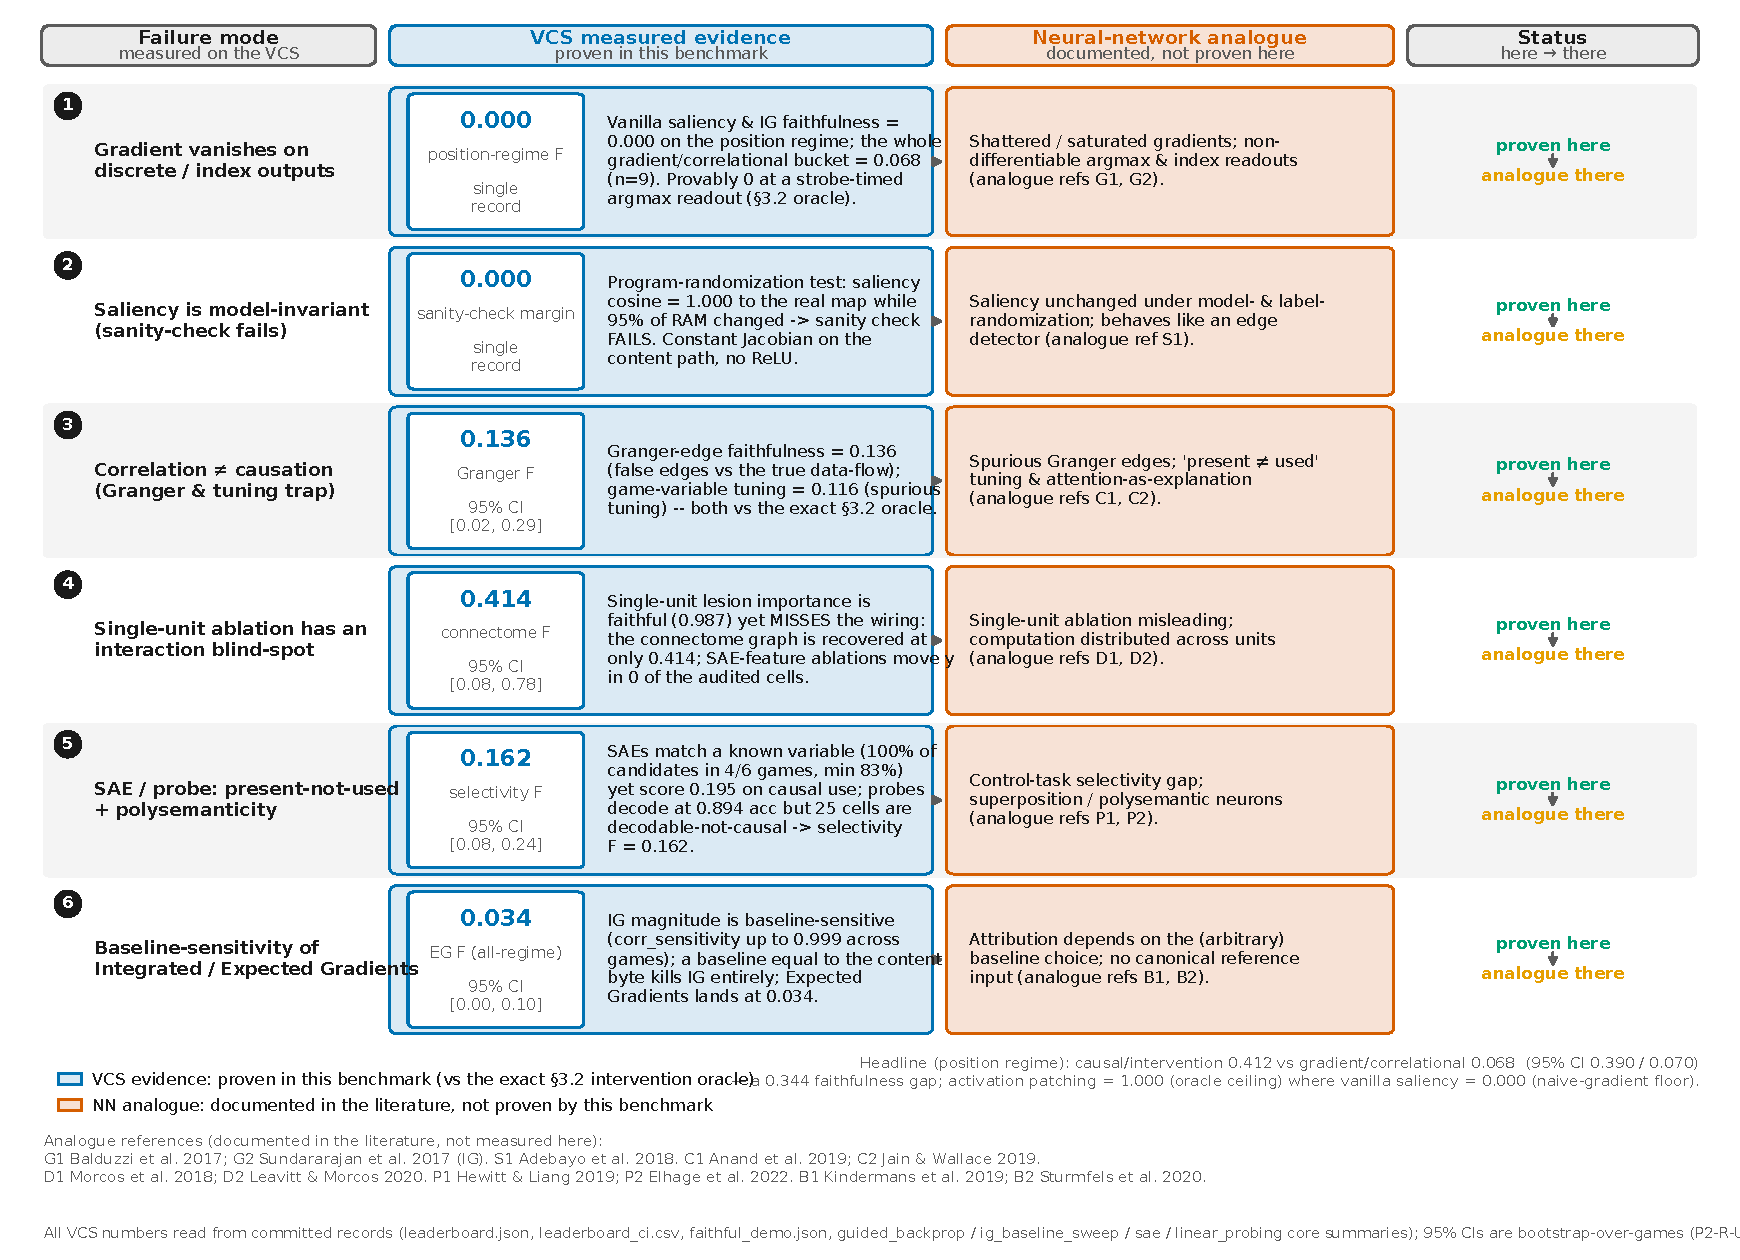
\includegraphics[width=\textwidth]{../figures/fig5_representativeness_map_full.pdf}
\caption{\textbf{Full VCS-to-NN representativeness map.} The full-density version of the
main-text map (Fig.~\ref{fig:representativeness}): each VCS failure mode is placed against its documented
neural-network analogue from the literature. The neural-network column records documented
analogues, not parallels proven by this benchmark; the oracle is the intervention oracle of
\Sectionname3.2, and the underlying per-method values trace to
\texttt{compare/out/leaderboard.json} via Sec.~\ref{supp:provenance}. Note that this full
map is the figure the simplified main-text version condenses.}
\label{supp:fig:repmap}
\end{figure}

\begin{figure}[t]
\centering
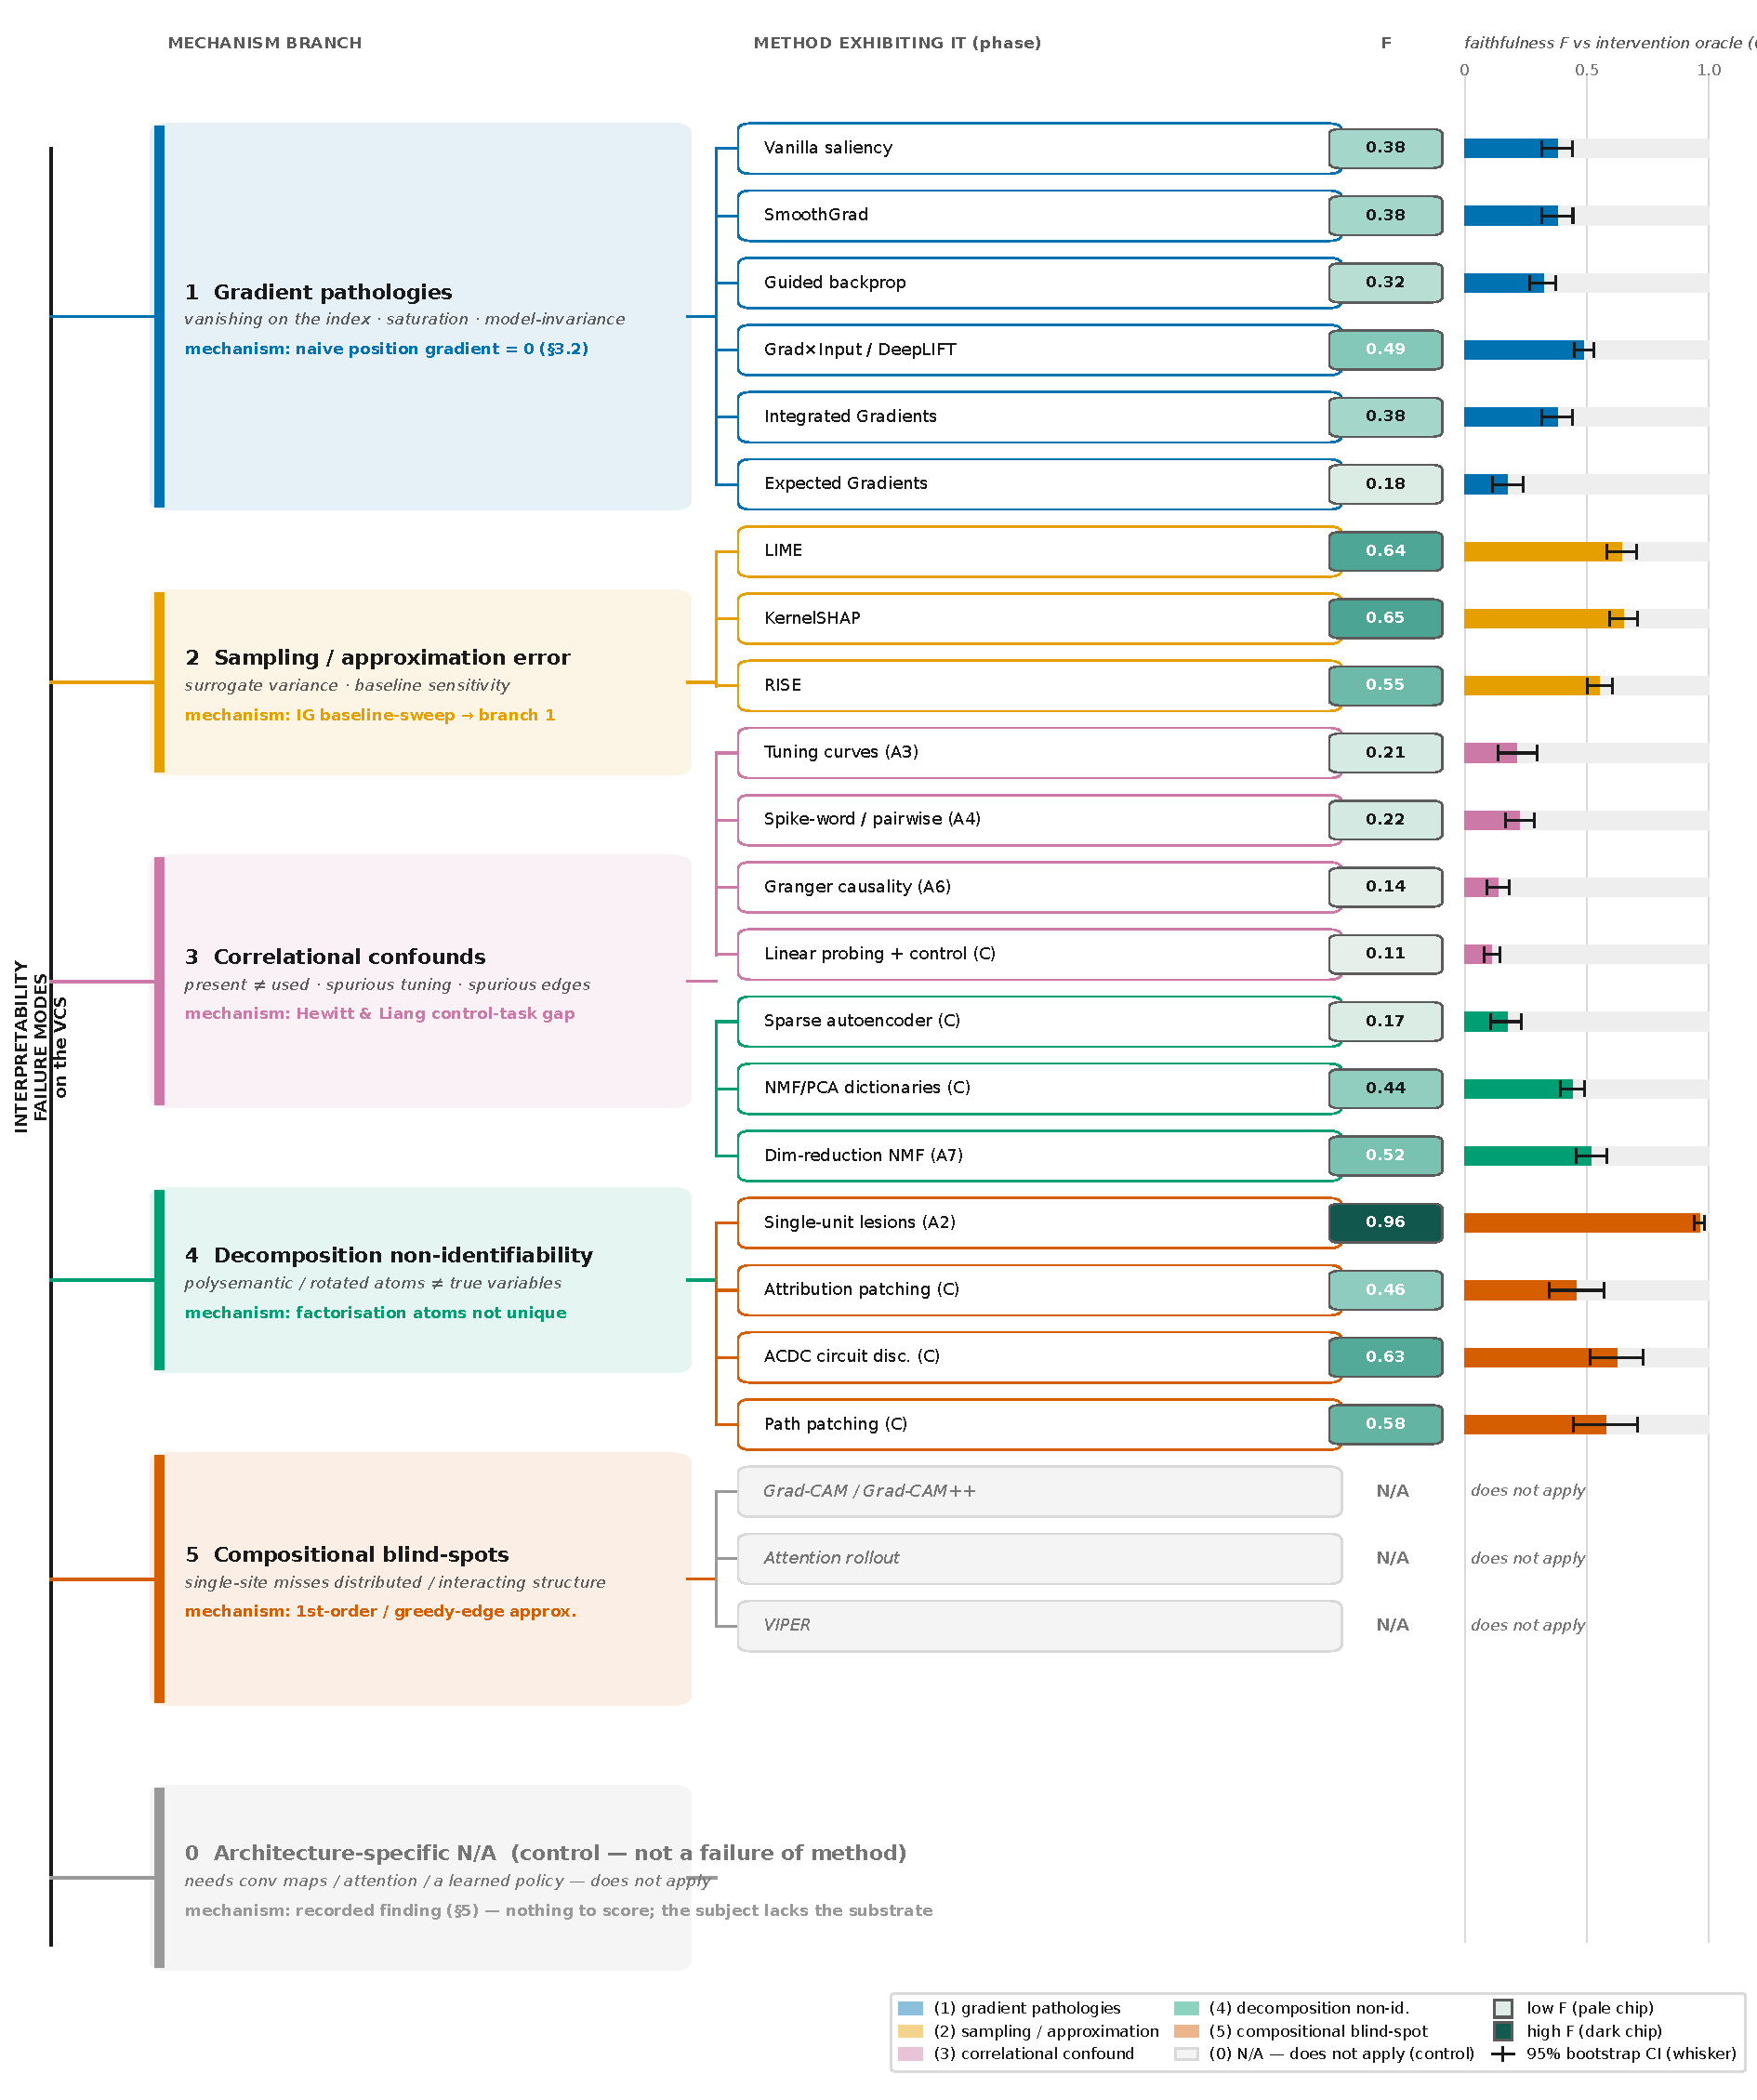
\includegraphics[width=\textwidth]{../figures/fig6_failure_taxonomy_full.pdf}
\caption{\textbf{Full failure taxonomy.} The full-density version of the main-text taxonomy
(Fig.~\ref{fig:taxonomy}): the families of interpretability failure observed on the machine, each annotated
with its faithfulness against the intervention oracle (\Sectionname3.2), reported as $F$ with its
$95\%$ bootstrap confidence interval. The leaf values trace to
\texttt{compare/out/leaderboard.json} and \texttt{leaderboard\_ci.csv} via
Sec.~\ref{supp:provenance}. Note that the gradient and correlational branches collapse on
the discrete position regime, where the naive gradient is provably zero (Prop.~\ref{prop:zero}).}
\label{supp:fig:taxonomy}
\end{figure}

\section{Plausibility-proxy rubric and its sensitivity}\label{supp:plausibility}

The plausibility axis of the leaderboard is a documented, tradition-level proxy, not a
human-subjects measurement. This section records how each value was assigned. It also shows
that the headline contrast does not depend on the particular numbers chosen. The Methods
(\Sectionname\ref{sec:triad}) name two reporting axes. Faithfulness is measured on the machine against the
intervention oracle of \Sectionname\ref{sec:oracle}. The plausibility proxy stands in for how convincing a
tradition's explanations are usually taken to be. We assign the proxy once per method
tradition, before any faithfulness score on our machine is computed, so it cannot be tuned to
the result. Its only job is to expose the danger zone of explanations that look convincing yet
are unfaithful. For that job it must be coarse, fixed in advance, and sourced rather than
precise.

The rubric assigns one proxy per tradition on a fixed five-step scale. It scores two
documented properties of each tradition's typical output and takes their average. The first
property is whether the explanation produces a dense, picture-like artifact that a reader sees
as an account of the computation. Heatmaps and saliency-style maps over the input are read as
convincing by construction. This is the perceptual-immediacy axis. The second property is
whether the field has historically treated the tradition's output as a self-evident
explanation rather than a hypothesis to be tested. This is the adoption-as-explanation axis. A
tradition that scores high on both, such as gradient saliency, receives a high proxy. A
tradition whose output is an austere intervention table or a circuit edge list, rarely
mistaken for a finished story, receives a low one. The scale is deliberately blunt,
$\{0.3,0.5,0.55,0.75,0.8,0.85,0.9\}$. A proxy meant to expose a danger zone gains nothing from
false precision, and a finer scale would invite over-reading. Every value in
Table~\ref{supp:tab:plausrubric} traces to the \jkey{plausibility_proxy} field of the
per-method rows in \texttt{compare/out/leaderboard.json}. The table only groups those rows by
tradition and records the rationale.

\begin{table}[t]
\centering
\caption{\textbf{Plausibility-proxy rubric.} The proxy assigned to each method tradition,
with the documented rationale. Values are the \jkey{plausibility_proxy} field of the
leaderboard rows (\texttt{compare/out/leaderboard.json}). They are tradition-level and fixed
before any faithfulness score is computed, so the proxy cannot be tuned to the measured
faithfulness. A higher value means an explanation that the field tends to find more
convincing, not one that is more faithful. The oracle (\Sectionname\ref{sec:oracle}) is the positive control and
is not a method under test.}
\label{supp:tab:plausrubric}
\begin{tabular}{@{}llp{6.4cm}@{}}
\toprule
Tradition & Proxy & Rationale (documented basis) \\
\midrule
gradient        & $0.90$ & Dense input-space heatmaps read as a visual account of the
                            decision; the most widely adopted XAI outputs, routinely shown
                            as if self-explanatory. \\
probing         & $0.85$ & A trained decoder that ``finds'' a concept reads as evidence the
                            concept is used; high adoption, though decodability is not
                            causal use. \\
correlational   & $0.80$ & Tuning curves and coupling spectra match the neuroscience idiom
                            of a convincing single-unit account. \\
dim.\ reduction & $0.75$ & Low-dimensional factors and dictionary atoms look like a clean
                            summary of the representation. \\
intervention    & $0.55$ & Occlusion and counterfactual outputs are quantitative tables, less
                            immediately picture-like, treated as tests rather than stories. \\
causal          & $0.50$ & Circuit edge lists and patching results are austere artifacts
                            rarely mistaken for a finished narrative. \\
descriptive     & $0.30$ & Whole-state recording is an explicit non-explanation: it withholds
                            nothing and reads as a dump, not an account. \\
\midrule
oracle (control)& $1.00$ & The \Sectionname\ref{sec:oracle} ground truth by construction; positive control, not a
                            method under test. \\
\bottomrule
\end{tabular}
\end{table}

The paper draws a contrast between this proxy and measured faithfulness. On the committed
records the two move in opposite directions. Across the thirty methods under test the Spearman
rank correlation between faithfulness and the proxy is $-0.36$, a negative association.
The traditions the field finds most convincing are, on this machine, among the least faithful.
Eight methods fall in the danger zone, defined here as a proxy of at least $0.70$ together
with a faithfulness below $0.40$. They include the correlational neuroscience methods, Expected
Gradients, guided backprop, linear probing, and the sparse autoencoder. The per-method extreme
makes the point sharply. Vanilla saliency has the highest proxy, $0.9$, yet scores faithfulness
$0.115$ on the position regime. Activation patching has a lower proxy, $0.5$, and scores $1.0$.
Here the less faithful method is the more plausible one. These figures are produced by
\texttt{tools/xai\_study/compare/plausibility\_sensitivity.py} from the leaderboard and
recorded in \texttt{compare/out/plausibility\_sensitivity.csv}.

A proxy fixed by a coarse rubric raises the question of whether the contrast is an artifact of
the particular numbers. The answer is that it is not. We perturb the proxy under four
deterministic schemes and recompute the relationship each time. The analysis uses fixed,
index-keyed offsets rather than random draws, so it re-derives bit-for-bit. The first scheme
adds a fixed per-method jitter of magnitude $\sigma\in\{0.05,0.1,0.2\}$, alternating in sign by
row. The second compresses every proxy toward the common mean by a fraction $\sigma$, which
preserves the rank order of traditions. The third uses the same index-keyed offsets at
$\sigma\in\{0.1,0.2\}$, large enough to swap neighbouring traditions' ranks. The fourth drops
one whole tradition at a time and recomputes on the remainder. Across all fourteen
perturbations the rank correlation between faithfulness and proxy stays negative. It ranges
from $-0.76$ to $-0.08$. The danger zone stays populated, with
between four and ten methods. The per-method anchor sign holds in every scheme where both
anchor methods are present, the more plausible saliency remaining the less faithful. Two runs
bound the range. The strongest is the leave-the-gradient-tradition-out run. It removes the most
plausible and least faithful block at once, and still leaves six danger-zone methods and a rank
correlation of $-0.76$. The weakest is the leave-the-causal-tradition-out run, where the
correlation falls to $-0.08$, close to zero; removing the faithful causal block flattens the
association, so the contrast is carried in part by that block. Table~\ref{supp:tab:plaussens}
reports the full sweep. The contrast keeps its sign under every alternative proxy assignment we
tried: plausibility and faithfulness are not the same axis, and high plausibility is no
guarantee of faithfulness.

\begin{table}[t]
\centering
\caption{\textbf{Proxy-sensitivity sweep.} The faithfulness-versus-proxy relationship under
each perturbation, from \texttt{compare/out/plausibility\_sensitivity.csv}. ``$\rho$'' is the
Spearman rank correlation between faithfulness and proxy over the methods present. ``danger''
is the count of high-proxy ($\geq0.70$), low-faithfulness ($<0.40$) methods. ``anchor'' is
$1$ when the more plausible saliency is the less faithful of the saliency/activation-patching
pair, and blank where a leave-one-out run removes an anchor. The baseline rubric is the first
row. Across every scheme the correlation stays negative and the danger zone stays populated.}
\label{supp:tab:plaussens}
\begin{tabular}{@{}llrrrc@{}}
\toprule
Scheme & Param & $n$ & $\rho$ & Danger & Anchor \\
\midrule
baseline                & ---           & 30 & $-0.36$ &  8 & 1 \\
additive jitter         & $\sigma=0.05$ & 30 & $-0.40$ &  8 & 1 \\
additive jitter         & $\sigma=0.10$ & 30 & $-0.41$ &  8 & 1 \\
additive jitter         & $\sigma=0.20$ & 30 & $-0.42$ & 10 & 1 \\
rank-preserving         & $\sigma=0.10$ & 30 & $-0.36$ &  8 & 1 \\
rank-preserving         & $\sigma=0.20$ & 30 & $-0.36$ &  8 & 1 \\
rank-jittering          & $\sigma=0.10$ & 30 & $-0.41$ &  8 & 1 \\
rank-jittering          & $\sigma=0.20$ & 30 & $-0.42$ & 10 & 1 \\
leave-out causal        & ---           & 24 & $-0.08$ &  8 & \\
leave-out correlational & ---           & 26 & $-0.40$ &  4 & 1 \\
leave-out descriptive   & ---           & 29 & $-0.29$ &  8 & 1 \\
leave-out dim.\ red.    & ---           & 27 & $-0.34$ &  7 & 1 \\
leave-out gradient      & ---           & 20 & $-0.76$ &  6 & \\
leave-out intervention  & ---           & 25 & $-0.34$ &  8 & 1 \\
leave-out probing       & ---           & 29 & $-0.36$ &  7 & 1 \\
\bottomrule
\end{tabular}
\end{table}

 into main.tex). It is also
%% a self-contained \input target: the six S-files below carry all SI content the main
%% paper promises (improvement_instructions P0#2, P0#4; P1#13, P1#14, P1#21; P3#35, P3#36).
%%
%% It re-uses, but does not re-derive, the §3 F/S/M definitions (S03 is authoritative)
%% and the canonical method count "30 interpretability methods + the oracle positive
%% control = 31 rows" (S07 is authoritative). Every reported number traces to a committed
%% record under tools/xai_study/compare/out/ (verifiable via the §6.5 traceability table
%% of REPRODUCIBILITY.md and re-derived by S5 below).
%%
%% Standalone compile (for review, before R6 wires it into main): wrap this file in the
%% sn-jnl preamble of a scratch driver (\documentclass[sn-nature,pdflatex]{sn-jnl} +
%% graphicx, booktabs, multirow, amsmath, longtable) and %% supplement.tex — Supplementary Information for Paper 2 (xai_2_interpretability).
%%
%% SCRUM note (P2-R-SUPP): this fragment is \input{} into the main paper by the SM
%% integration write (R6 wires %% supplement.tex — Supplementary Information for Paper 2 (xai_2_interpretability).
%%
%% SCRUM note (P2-R-SUPP): this fragment is \input{} into the main paper by the SM
%% integration write (R6 wires %% supplement.tex — Supplementary Information for Paper 2 (xai_2_interpretability).
%%
%% SCRUM note (P2-R-SUPP): this fragment is \input{} into the main paper by the SM
%% integration write (R6 wires \input{supplement/supplement} into main.tex). It is also
%% a self-contained \input target: the six S-files below carry all SI content the main
%% paper promises (improvement_instructions P0#2, P0#4; P1#13, P1#14, P1#21; P3#35, P3#36).
%%
%% It re-uses, but does not re-derive, the §3 F/S/M definitions (S03 is authoritative)
%% and the canonical method count "30 interpretability methods + the oracle positive
%% control = 31 rows" (S07 is authoritative). Every reported number traces to a committed
%% record under tools/xai_study/compare/out/ (verifiable via the §6.5 traceability table
%% of REPRODUCIBILITY.md and re-derived by S5 below).
%%
%% Standalone compile (for review, before R6 wires it into main): wrap this file in the
%% sn-jnl preamble of a scratch driver (\documentclass[sn-nature,pdflatex]{sn-jnl} +
%% graphicx, booktabs, multirow, amsmath, longtable) and \input{supplement}; the tables
%% render without overfull boxes and the two SI figures resolve from ../figures/.

\clearpage
\appendix

%% Breakable monospaced JSON key: lets long under_scored keys wrap inside narrow table
%% columns. Used by S5 (number provenance). Defined here so the S-files stay self-contained.
\providecommand{\jkey}[1]{\texttt{\expandafter\jkeyaux#1\relax}}
\makeatletter
\def\jkeyaux#1{\ifx\relax#1\else
  \ifx_#1\discretionary{}{}{}\char`\_\else
    \ifx.#1\discretionary{}{}{}.\else#1\fi\fi
  \expandafter\jkeyaux\fi}
\makeatother

\section*{Supplementary Information}
\setcounter{table}{0}
\setcounter{figure}{0}
\renewcommand{\thetable}{S\arabic{table}}
\renewcommand{\thefigure}{S\arabic{figure}}
\renewcommand{\thesection}{S\arabic{section}}
\setcounter{section}{0}

This Supplementary Information records what the main paper summarizes. We give the
per-method protocols (\Sectionname\ref{supp:protocols}) and the leaderboard schema with its glossary
(\Sectionname\ref{supp:schema}). We give the coverage and applicability of every method across games
and output regimes (\Sectionname\ref{supp:coverage}). We map each headline claim to its evidence
(\Sectionname\ref{supp:claims}). We trace the provenance of every headline number down to the record
file and command that produced it (\Sectionname\ref{supp:provenance}). We state plainly what the
paper does not claim (\Sectionname\ref{supp:notclaimed}). We give the plausibility-proxy rubric and
its sensitivity analysis (\Sectionname\ref{supp:plausibility}). The main text shows simplified forms
of two diagnostic figures; we reproduce both here at full resolution
(Figs.~\ref{supp:fig:repmap} and~\ref{supp:fig:taxonomy}).
The correctness triad $\mathrm{F}\wedge\mathrm{S}\wedge\mathrm{M}$ used throughout is the
one defined in the main Methods (\Sectionname\ref{sec:triad}); we reference it here rather than restating it. The
benchmark scores 30 interpretability methods together with the intervention oracle (\Sectionname\ref{sec:oracle})
as a positive control, for 31 leaderboard rows in total.

\input{supplement/S1_per_method_protocols}
\input{supplement/S2_benchmark_schema}
\input{supplement/S3_coverage_applicability}
\input{supplement/S4_claims_evidence}
\input{supplement/S5_number_provenance}
\input{supplement/S6_not_claimed}
\input{supplement/S7_plausibility}
 into main.tex). It is also
%% a self-contained \input target: the six S-files below carry all SI content the main
%% paper promises (improvement_instructions P0#2, P0#4; P1#13, P1#14, P1#21; P3#35, P3#36).
%%
%% It re-uses, but does not re-derive, the §3 F/S/M definitions (S03 is authoritative)
%% and the canonical method count "30 interpretability methods + the oracle positive
%% control = 31 rows" (S07 is authoritative). Every reported number traces to a committed
%% record under tools/xai_study/compare/out/ (verifiable via the §6.5 traceability table
%% of REPRODUCIBILITY.md and re-derived by S5 below).
%%
%% Standalone compile (for review, before R6 wires it into main): wrap this file in the
%% sn-jnl preamble of a scratch driver (\documentclass[sn-nature,pdflatex]{sn-jnl} +
%% graphicx, booktabs, multirow, amsmath, longtable) and %% supplement.tex — Supplementary Information for Paper 2 (xai_2_interpretability).
%%
%% SCRUM note (P2-R-SUPP): this fragment is \input{} into the main paper by the SM
%% integration write (R6 wires \input{supplement/supplement} into main.tex). It is also
%% a self-contained \input target: the six S-files below carry all SI content the main
%% paper promises (improvement_instructions P0#2, P0#4; P1#13, P1#14, P1#21; P3#35, P3#36).
%%
%% It re-uses, but does not re-derive, the §3 F/S/M definitions (S03 is authoritative)
%% and the canonical method count "30 interpretability methods + the oracle positive
%% control = 31 rows" (S07 is authoritative). Every reported number traces to a committed
%% record under tools/xai_study/compare/out/ (verifiable via the §6.5 traceability table
%% of REPRODUCIBILITY.md and re-derived by S5 below).
%%
%% Standalone compile (for review, before R6 wires it into main): wrap this file in the
%% sn-jnl preamble of a scratch driver (\documentclass[sn-nature,pdflatex]{sn-jnl} +
%% graphicx, booktabs, multirow, amsmath, longtable) and \input{supplement}; the tables
%% render without overfull boxes and the two SI figures resolve from ../figures/.

\clearpage
\appendix

%% Breakable monospaced JSON key: lets long under_scored keys wrap inside narrow table
%% columns. Used by S5 (number provenance). Defined here so the S-files stay self-contained.
\providecommand{\jkey}[1]{\texttt{\expandafter\jkeyaux#1\relax}}
\makeatletter
\def\jkeyaux#1{\ifx\relax#1\else
  \ifx_#1\discretionary{}{}{}\char`\_\else
    \ifx.#1\discretionary{}{}{}.\else#1\fi\fi
  \expandafter\jkeyaux\fi}
\makeatother

\section*{Supplementary Information}
\setcounter{table}{0}
\setcounter{figure}{0}
\renewcommand{\thetable}{S\arabic{table}}
\renewcommand{\thefigure}{S\arabic{figure}}
\renewcommand{\thesection}{S\arabic{section}}
\setcounter{section}{0}

This Supplementary Information records what the main paper summarizes. We give the
per-method protocols (\Sectionname\ref{supp:protocols}) and the leaderboard schema with its glossary
(\Sectionname\ref{supp:schema}). We give the coverage and applicability of every method across games
and output regimes (\Sectionname\ref{supp:coverage}). We map each headline claim to its evidence
(\Sectionname\ref{supp:claims}). We trace the provenance of every headline number down to the record
file and command that produced it (\Sectionname\ref{supp:provenance}). We state plainly what the
paper does not claim (\Sectionname\ref{supp:notclaimed}). We give the plausibility-proxy rubric and
its sensitivity analysis (\Sectionname\ref{supp:plausibility}). The main text shows simplified forms
of two diagnostic figures; we reproduce both here at full resolution
(Figs.~\ref{supp:fig:repmap} and~\ref{supp:fig:taxonomy}).
The correctness triad $\mathrm{F}\wedge\mathrm{S}\wedge\mathrm{M}$ used throughout is the
one defined in the main Methods (\Sectionname\ref{sec:triad}); we reference it here rather than restating it. The
benchmark scores 30 interpretability methods together with the intervention oracle (\Sectionname\ref{sec:oracle})
as a positive control, for 31 leaderboard rows in total.

\input{supplement/S1_per_method_protocols}
\input{supplement/S2_benchmark_schema}
\input{supplement/S3_coverage_applicability}
\input{supplement/S4_claims_evidence}
\input{supplement/S5_number_provenance}
\input{supplement/S6_not_claimed}
\input{supplement/S7_plausibility}
; the tables
%% render without overfull boxes and the two SI figures resolve from ../figures/.

\clearpage
\appendix

%% Breakable monospaced JSON key: lets long under_scored keys wrap inside narrow table
%% columns. Used by S5 (number provenance). Defined here so the S-files stay self-contained.
\providecommand{\jkey}[1]{\texttt{\expandafter\jkeyaux#1\relax}}
\makeatletter
\def\jkeyaux#1{\ifx\relax#1\else
  \ifx_#1\discretionary{}{}{}\char`\_\else
    \ifx.#1\discretionary{}{}{}.\else#1\fi\fi
  \expandafter\jkeyaux\fi}
\makeatother

\section*{Supplementary Information}
\setcounter{table}{0}
\setcounter{figure}{0}
\renewcommand{\thetable}{S\arabic{table}}
\renewcommand{\thefigure}{S\arabic{figure}}
\renewcommand{\thesection}{S\arabic{section}}
\setcounter{section}{0}

This Supplementary Information records what the main paper summarizes. We give the
per-method protocols (\Sectionname\ref{supp:protocols}) and the leaderboard schema with its glossary
(\Sectionname\ref{supp:schema}). We give the coverage and applicability of every method across games
and output regimes (\Sectionname\ref{supp:coverage}). We map each headline claim to its evidence
(\Sectionname\ref{supp:claims}). We trace the provenance of every headline number down to the record
file and command that produced it (\Sectionname\ref{supp:provenance}). We state plainly what the
paper does not claim (\Sectionname\ref{supp:notclaimed}). We give the plausibility-proxy rubric and
its sensitivity analysis (\Sectionname\ref{supp:plausibility}). The main text shows simplified forms
of two diagnostic figures; we reproduce both here at full resolution
(Figs.~\ref{supp:fig:repmap} and~\ref{supp:fig:taxonomy}).
The correctness triad $\mathrm{F}\wedge\mathrm{S}\wedge\mathrm{M}$ used throughout is the
one defined in the main Methods (\Sectionname\ref{sec:triad}); we reference it here rather than restating it. The
benchmark scores 30 interpretability methods together with the intervention oracle (\Sectionname\ref{sec:oracle})
as a positive control, for 31 leaderboard rows in total.

\section{Per-method protocols}\label{supp:protocols}

This section records five things for each method under test. It records the exact objects the
method consumes and produces, the reference it is scored against, its sampling or optimization
budget, the metric that turns its output into a faithfulness score, and the committed record
file (version-controlled, in the released repository) that holds the per-game results. All methods share one evaluation contract. We state that
contract once and then specialize it per method. Every method receives the same bit-exact VCS
state on each game of the scored set. We state the contract on the six core games
(\texttt{breakout}, \texttt{ms\_pacman}, \texttt{pong}, \texttt{qbert}, \texttt{seaquest},
\texttt{space\_invaders}), which carry the full tiered ground truth and the exact oracle and
serve as the running example; the aggregate leaderboard scores extend the identical protocol
to the 42-game scored set of \Sectionname\ref{supp:scoredset}. That state is not the boot screen.
It is a shared gameplay state, produced by a single seeded random-action stream (seed~$0$) run
for a $90$-frame prefix and then rolled forward for a $15$-frame analysis horizon. The stream is
deterministic, so every method sees the identical state on each game, and the run is asserted
bit-exact per game. An oracle cause-density gate screens the state before any method runs. The
gate counts how many candidate causes move the output above a floor and rejects states with too
few, so a near-flat oracle column cannot pass. This gate is what turns a degenerate frame into a
usable one; on \texttt{seaquest} it raises the count of live candidate causes from $2$ to $19$.
The candidate-cause set is the machine's own state. This set is the RAM bytes together with the
CPU registers and the TIA and RIOT registers exposed by the substrate. The output every method
attributes over is a shared screen-buffer region read at the end of the analysis horizon, not a
single hand-picked pixel. The reference is the intervention oracle of \Sectionname\ref{sec:oracle},
evaluated by exact re-runs of the emulator under $\mathrm{do}(u)$. A method that
cannot be applied to a given output regime is recorded as not-applicable rather than scored
as zero. An empty result is therefore never read as a wrong one. Faithfulness is the F
axis of the main-text triad (\Sectionname\ref{sec:triad}); we reference that definition and do not restate it.
Records live under \texttt{tools/xai\_study/<phase>/out/}; the aggregate they feed is
\texttt{tools/xai\_study/compare/out/leaderboard.json}.
Table~\ref{supp:leaderboard} consolidates the triad scores for all thirty methods and the
oracle positive control in one place; the per-method protocols follow.

\begin{table*}[t]
\centering
\caption{\textbf{Consolidated leaderboard: all methods, all triad axes.} One row per method
across the three phases, plus the intervention oracle as a positive control. $F$ is
faithfulness (Pearson correlation against the oracle, with the bootstrap-over-games 95\% CI in
brackets), $S$ is sufficiency, $M$ is minimality, all as defined in \Sectionname\ref{sec:triad};
Plaus is the elicited plausibility prior and $n$ is the number of scored games. Attribution
methods that emit only a saliency have no defined $S$ or $M$ and are marked ``---''; A5
(field potentials) and A7 (dimensionality reduction) likewise lack the $S$/$M$ decomposition.
Values are transcribed from \texttt{tools/xai\_study/compare/out/leaderboard.json} (the
committed numbers of record).}
\label{supp:leaderboard}
\footnotesize
\setlength{\tabcolsep}{4pt}
\begin{tabularx}{\textwidth}{@{}Xccccccc@{}}
\toprule
Method & Phase & Tradition & $F$ (95\% CI) & $S$ & $M$ & Plaus & $n$ \\
\midrule
A1 connectomics & A & intervention & 0.207 [0.130, 0.293] & 0.971 & 0.967 & 0.55 & 35 \\
A2 lesions & A & intervention & 0.965 [0.942, 0.983] & 0.591 & 1.000 & 0.55 & 42 \\
A3 tuning curves & A & correlational & 0.213 [0.136, 0.295] & 0.200 & 0.928 & 0.80 & 42 \\
A4 spike-word / pairwise & A & correlational & 0.225 [0.166, 0.283] & 0.133 & 0.363 & 0.80 & 34 \\
A5 field potentials & A & correlational & 0.376 [0.323, 0.428] & --- & --- & 0.80 & 40 \\
A6 Granger & A & correlational & 0.136 [0.091, 0.184] & 0.884 & 0.647 & 0.80 & 35 \\
A7 dim.\ reduction & A & dim.\ red. & 0.519 [0.457, 0.581] & --- & --- & 0.75 & 42 \\
A8 whole-state & A & descriptive & 1.000 [1.000, 1.000] & 1.000 & 0.075 & 0.30 & 42 \\
\midrule
Vanilla saliency & B & gradient & 0.380 [0.316, 0.445] & --- & --- & 0.90 & 42 \\
smoothgrad & B & gradient & 0.380 [0.317, 0.445] & --- & --- & 0.90 & 42 \\
Guided backprop & B & gradient & 0.322 [0.267, 0.375] & --- & --- & 0.90 & 42 \\
Grad$\times$Input / DeepLIFT & B & gradient & 0.486 [0.448, 0.526] & --- & --- & 0.90 & 42 \\
Integrated Gradients & B & gradient & 0.379 [0.314, 0.444] & --- & --- & 0.90 & 42 \\
Expected Gradients & B & gradient & 0.175 [0.110, 0.240] & --- & --- & 0.90 & 42 \\
kernelshap & B & gradient & 0.652 [0.596, 0.709] & --- & --- & 0.90 & 42 \\
lime & B & gradient & 0.644 [0.582, 0.705] & --- & --- & 0.90 & 42 \\
rise & B & gradient & 0.552 [0.500, 0.600] & --- & --- & 0.90 & 42 \\
occlusion & B & intervention & 0.687 [0.624, 0.746] & --- & --- & 0.55 & 42 \\
Extremal perturbation & B & intervention & 0.461 [0.410, 0.513] & --- & --- & 0.55 & 42 \\
On-distribution counterfactual & B & intervention & 0.433 [0.343, 0.522] & --- & --- & 0.55 & 42 \\
\midrule
Activation patching & C & causal & 1.000 [1.000, 1.000] & --- & --- & 0.50 & 42 \\
Causal scrubbing & C & causal & 0.979 [0.940, 1.000] & 0.979 & 0.814 & 0.50 & 42 \\
Interchange interventions (DAS) & C & causal & 1.000 [1.000, 1.000] & --- & --- & 0.50 & 42 \\
Logit / tuned lens & C & causal & 0.820 [0.768, 0.871] & --- & 0.224 & 0.50 & 42 \\
Path patching & C & causal & 0.580 [0.452, 0.710] & --- & --- & 0.50 & 42 \\
ACDC & C & causal & 0.625 [0.514, 0.730] & 0.299 & 1.000 & 0.50 & 35 \\
Attribution patching & C & gradient & 0.456 [0.345, 0.573] & --- & --- & 0.90 & 42 \\
Linear probing (+ control) & C & probing & 0.240 [0.153, 0.346] & --- & 0.932 & 0.85 & 42 \\
NMF / PCA dictionaries & C & dim.\ red. & 0.102 [0.049, 0.160] & 0.751 & 0.966 & 0.75 & 42 \\
Sparse autoencoder & C & dim.\ red. & 0.153 [0.096, 0.218] & 0.183 & 0.934 & 0.75 & 40 \\
\midrule
Intervention oracle & --- & oracle & 1.000 [1.000, 1.000] & 1.000 & 1.000 & 1.00 & 1 \\
\bottomrule
\end{tabularx}
\end{table*}

The neuroscience analyses (Phase~A) treat the running machine as a brain. It asks how far
each classical analysis recovers the known mechanism on the shared gameplay state. Each
method's baseline is the exact data-flow graph or causal role that the substrate makes
available. Its budget is the scored set (\Sectionname\ref{supp:scoredset}) unless noted,
with the six-game core as the running example, and its scoring metric is named in
Table~\ref{supp:tab:phaseA}. One core cell is honestly degenerate. On \texttt{ms\_pacman} the
pairwise analysis (A4) finds no coupled candidate pair to score at that frame, so its
\texttt{ms\_pacman} value is uninformative rather than a failure; the other five games carry
it.

\begin{table}[t]
\centering
\caption{\textbf{Phase~A protocols (neuroscience analyses).} One row per method. The columns
give the input it reads, the reference it is scored against, the sampling or intervention
budget, the scoring metric, and the committed record. All eight run on the scored set
(\Sectionname\ref{supp:scoredset}), with the six core games as the running example;
faithfulness is the F axis of \Sectionname\ref{sec:triad}. The whole-state recording (A8) is included as a
descriptive upper bound on coverage. Its faithfulness $F$ is trivial, so we read it for its
minimality $M$.}
\label{supp:tab:phaseA}
\scriptsize
\setlength{\tabcolsep}{4pt}
\begin{tabular}{@{}p{1.7cm}p{2.6cm}p{1.9cm}p{2.6cm}p{1.0cm}@{}}
\toprule
Method & Input / candidate causes & Reference & Scoring metric & Record \\
\midrule
A1 connectomics & RAM/register activity over trajectory & data-flow graph & data-flow graph $F_1$ vs.\ oracle & A1 \\
A2 lesions & single-cell knockouts via $\mathrm{do}(u)$ & true causal role & lesion-importance $\rho$ vs.\ role & A2 \\
A3 tuning curves & per-cell response vs.\ variable & variable coupling & $1-$ spurious-tuning rate & A3 \\
A4 spike-word / pairwise & pairwise cell correlations & true coupling & corr.\ $\rho$ vs.\ coupling & A4 \\
A5 field potentials & pooled-activity spectra & true causal share & $1-$ clock-explained var. & A5 \\
A6 Granger & directed lag structure & true data-flow & $1-$ false-edge rate & A6 \\
A7 dim.\ reduction & NMF/PCA over activity & known variables & NMF matched-component frac. & A7 \\
A8 whole-state & full state record & oracle decomp. & minimality $M$ vs.\ oracle & A8 \\
\bottomrule
\end{tabular}

\smallskip
\noindent\scriptsize Records: \texttt{tools/xai\_study/phaseA\_kording/out/A\{1..8\}\_*}; all
eight run on the 42-game scored set (\Sectionname\ref{supp:scoredset}), with the six core
games as the running example (\jkey{n_games} per method in \jkey{leaderboard.json}).
\end{table}

The attribution methods (Phase~B) run the everyday XAI toolbox over the same gameplay state.
These methods produce a real-valued saliency or attribution over the candidate-cause set.
We score that output by Pearson correlation against the oracle attribution. The gradient family
runs with the bilinear sub-pixel sampler turned on, so it is scored on a real position gradient
and not on the naive one. The naive gradient of the discrete position output is provably zero
(Prop.~\ref{prop:zero}); the sampler restores a finite gradient, but the restored gradient is
low and mixed in faithfulness rather than a fix. Expected Gradients draws its reference pool
from the states of the same seeded gameplay trajectory, not from a synthetic baseline. Two cells
are honestly degenerate and recorded as such. The on-distribution counterfactual returns a zero
delta on \texttt{space\_invaders}, \texttt{ms\_pacman}, and \texttt{qbert}, where its perturbation
does not move the shared output at that frame; those cells are marked not-valid rather than
scored. Expected Gradients scores low on the content regime of every game except \texttt{pong},
because the causal byte it should land on is static there. The budgets that matter are the
Monte-Carlo or perturbation counts of the sampling estimators, recorded per method in
Table~\ref{supp:tab:phaseB}. The seed-dispersion of the stochastic members is carried in
\texttt{leaderboard\_ci.csv} (\texttt{seed\_sd}, \texttt{seed\_sd\_source}) and reproduced
in \Sectionname\ref{supp:provenance}.

\begin{table}[t]
\centering
\caption{\textbf{Phase~B protocols (attribution methods).} Each method emits a saliency over
the candidate-cause set. We score it by Pearson correlation against the oracle attribution
(\Sectionname\ref{sec:oracle}). The reference is shared and the budget is the scored set of
\Sectionname\ref{supp:scoredset} (six core games as the running example). The budget column records the
sampling or perturbation count that drives each estimator. The seed column flags which
methods carry an independent-seed dispersion in \texttt{leaderboard\_ci.csv}.}
\label{supp:tab:phaseB}
\scriptsize
\setlength{\tabcolsep}{4pt}
\begin{tabular}{@{}p{2.9cm}p{1.75cm}p{4.3cm}p{1.15cm}@{}}
\toprule
Method & Tradition & Budget / hyperparameters & Seed sd \\
\midrule
Vanilla saliency & gradient & single backward pass & --- \\
smoothgrad & gradient & noise-averaged gradient; $\sigma$-robustness committed & 0.0 \\
Guided backprop & gradient & single guided pass & --- \\
Grad$\times$Input / DeepLIFT & gradient & DeepLIFT reference-difference & --- \\
Integrated Gradients & gradient & path integral, baseline = zero state & --- \\
Expected Gradients & gradient & expectation over baselines (refits) & yes \\
kernelshap & gradient & Monte-Carlo coalition sampling ($\propto 1/\sqrt{N}$) & 0.017 \\
lime & gradient & local linear fit, perturbation refits & 0.029 \\
rise & gradient & random-mask Monte-Carlo ($\propto 1/\sqrt{N}$) & 0.051 \\
occlusion & intervention & exhaustive single-cell masking & --- \\
Extremal perturbation & intervention & optimized mask, area-constrained & --- \\
On-distribution counterfactual & intervention & on-manifold $\mathrm{do}(u)$ resampling & --- \\
\bottomrule
\end{tabular}

\smallskip
\noindent\scriptsize Records: \texttt{tools/xai\_study/phaseB\_attribution/out/}; all twelve run
on the 42-game scored set (\Sectionname\ref{supp:scoredset}), six core games as the running
example, and are scored by Pearson correlation against the oracle (\Sectionname\ref{sec:oracle}). Seed
sd is the independent-seed dispersion from \texttt{leaderboard\_ci.csv}.
\end{table}

The mechanistic methods (Phase~C) are built to recover circuits. Each is scored
against the true data-flow or the exact recovered-minus-exact deviation. The causal members
of this phase are the ones that reach the oracle ceiling. We list their exact scoring metric
so that the ceiling is not read as a tautology. Each member is scored against the substrate's
known routine, and not against another method. Two members (NMF/PCA dictionaries and the
sparse autoencoder) are dimensionality-reduction methods carried here for comparison. The
sparse autoencoder has two aggregations that differ, which we reconcile in
\Sectionname\ref{supp:provenance}.

\begin{table}[t]
\centering
\caption{\textbf{Phase~C protocols (mechanistic methods).} Each method is scored against the
substrate's known circuit or the exact recovered-minus-exact deviation (\Sectionname\ref{sec:oracle}), and not
against another method. This is what keeps the oracle ceiling non-circular. The probing and
dictionary-learning members are included for comparison with the causal members.}
\label{supp:tab:phaseC}
\scriptsize
\setlength{\tabcolsep}{4pt}
\begin{tabular}{@{}p{3.4cm}p{1.4cm}p{5.2cm}@{}}
\toprule
Method & Tradition & Scoring metric \\
\midrule
Activation patching & causal & $\max|\text{recovered}-\text{exact}|$ vs.\ oracle \\
Causal scrubbing & causal & scrubbing-preserved performance \\
Interchange interventions (DAS) & causal & aligned interchange accuracy \\
Logit / tuned lens & causal & logit-lens fidelity to true intermediate \\
Path patching & causal & path-circuit $F_1$ vs.\ true routine \\
ACDC & causal & discovered-circuit best $F_1$ vs.\ data-flow \\
Attribution patching & gradient & corr.\ of approximation vs.\ exact patch \\
Linear probing (+ control) & probing & selectivity vs.\ control task \\
NMF / PCA dictionaries & dim.\ red. & matched-component fraction vs.\ vars \\
Sparse autoencoder & dim.\ red. & feature-variable matched fraction \\
\bottomrule
\end{tabular}

\smallskip
\noindent\scriptsize Records: \texttt{tools/xai\_study/phaseC\_mechanistic/out/}; all ten run
on the 42-game scored set (\Sectionname\ref{supp:scoredset}), with the six core games as the
running example.
\end{table}

The intervention oracle is the positive control, not a method under test. It is the exact
$\mathrm{do}(u)$ ground truth of \Sectionname\ref{sec:oracle}, evaluated by re-running the bit-exact machine. It
attains $F=S=M=1.0$ by construction. Its record triple is the intervention oracle, the
content-path gradient oracle, and their cross-check
(\texttt{tools/xai\_study/ground\_truth/out/}). It anchors the ceiling against which every
other row is read, which is why it occupies the thirty-first leaderboard row.

\section{Benchmark schema and glossary}\label{supp:schema}

The leaderboard is built from a flat record schema. Stating it removes the ambiguity
about what a single number on the benchmark counts. Each method is run per game and writes a
per-game record under its phase's \texttt{out/} tree. The leaderboard aggregates those
records into one row per method by averaging over games. The schema columns of a leaderboard
row are given in Table~\ref{supp:tab:schema}. The aggregation rule is a mean over the
$n_{\text{games}}$ games. When a method emits several output records on one game, those records
are first reduced within that game. The faithfulness, sufficiency, and minimality columns
report the F, S, and M axes defined in \Sectionname\ref{sec:triad}. We do not re-derive those definitions here.

\begin{table}[t]
\centering
\caption{\textbf{Leaderboard row schema.} The columns of one row in
\texttt{compare/out/leaderboard.json} (\texttt{rows[\,]}) and its uncertainty companion
\texttt{leaderboard\_ci.csv}. The metric column names the per-method scoring function from
\Sectionname\ref{supp:protocols}; F, S, and M are the triad axes of \Sectionname\ref{sec:triad}. Aggregation is a mean
over $n_{\text{games}}$, with bootstrap confidence intervals over games (and, where present,
over records).}
\label{supp:tab:schema}
\footnotesize
\begin{tabular}{@{}p{3.0cm}p{8.4cm}@{}}
\toprule
Column & Meaning \\
\midrule
\texttt{phase} & phaseA\_kording, phaseB\_attribution, phaseC\_mechanistic, or ground\_truth \\
\texttt{method} & method identifier (the row key) \\
\texttt{tradition} & intervention, causal, gradient, correlational, \jkey{dim_reduction}, probing, descriptive, oracle \\
\jkey{n_games} & number of games the method was scored on (up to 42 for the scored set of \Sectionname\ref{supp:scoredset}; 1 for the oracle) \\
\jkey{n_records} & number of per-game output records aggregated into the row \\
\texttt{faithfulness} (F) & faithfulness vs.\ the intervention oracle (\Sectionname\ref{sec:oracle}), $[0,1]$, higher better \\
\jkey{faithfulness_ci95} & $95\%$ bootstrap CI half-width over games \\
\jkey{faithfulness_position_regime} & F restricted to the discrete sprite-position/index regime \\
\jkey{faithfulness_content_regime} & F restricted to the continuous content regime \\
\texttt{triad\_S} / \texttt{triad\_M} & sufficiency / minimality axes (\Sectionname\ref{sec:triad}), where applicable \\
\jkey{plausibility_proxy} & documented method-tradition proxy, $[0,1]$ --- not a human-subjects measurement \\
\jkey{is_positive_control} & 1 for the oracle row, 0 otherwise \\
\jkey{metric_names} & the per-method scoring function (\Sectionname\ref{supp:protocols}) \\
\texttt{commits} & the commit(s) at which the per-game records were produced \\
\bottomrule
\end{tabular}
\end{table}

We fix the vocabulary that the schema implies, because the review asked for a single
unambiguous method count. A \emph{method} is one interpretability technique, e.g.\
\texttt{vanilla\_saliency}. A \emph{method row} is its single aggregated line on the
leaderboard. A \emph{per-game record} is one method scored on one game, written under a phase
\texttt{out/} tree. An \emph{output record} is a per-game record for one output regime; a
method may emit several of these on one game. A \emph{family mean} is the average over the
members of a tradition family, e.g.\ causal/intervention. The \emph{oracle positive control}
is the exact $\mathrm{do}(u)$ ground truth of \Sectionname\ref{sec:oracle}, scored as a method to anchor the
ceiling. A \emph{not-applicable method} is one that does not apply to a given output regime;
it is recorded as N/A rather than as a zero. With this vocabulary the count is unambiguous.
The benchmark scores 30 interpretability methods together with the intervention
oracle as a positive control, for 31 leaderboard rows in total
(\texttt{leaderboard.json.n\_methods}~$=31$), aggregating 1773 per-game records over the
42-game scored set (\texttt{n\_per\_game\_records\_aggregated}~$=1773$): 8 methods in
Phase~A, 12 in Phase~B, 10 in Phase~C, and the one oracle row. This count is the canonical one
used in the abstract, the figures, and throughout this Supplement.

\section{Coverage and applicability}\label{supp:coverage}

The benchmark scores methods on a six-game core drawn from a larger bit-exact substrate. The
coverage table makes the scope of that choice explicit. Paper~1 validates the
differentiable VCS ports bit-for-bit against the \texttt{xitari} reference on all 64 Arcade
Learning Environment games, within a 30-frame RAM and 60-frame screen window. The
interpretability study reported here runs on the six games listed in
Table~\ref{supp:tab:coverage}. Every method is scored on a shared gameplay state, produced by
one seeded random-action stream (seed~$0$, $90$-frame prefix, $15$-frame analysis horizon), not
on the boot screen. This keeps the analysis inside the Paper~1 bit-exact window while giving the
oracle a rich, non-degenerate cause set to score against. We pick these six games because all
three tiers of ground truth (\Sectionname\ref{sec:tiers}) are available for them and the oracle is
exact. The remaining 58 games are
bit-exact substrate but are not scored here. Some fall outside the validated horizon for the
analyses we run. For others, the tiered labels they would need are not yet produced. They are
candidates for the larger sweep, and are not excluded for any methodological reason. The
horizon column records the validated window. The tier column records which of the three
ground-truth tiers (T1 exact intervention, T2 data-flow, T3 externally-supplied semantic
labels) is available.

\begin{table}[t]
\centering
\caption{\textbf{Core-game coverage.} The six core games carry exact tiered ground truth and
the full method battery. Faithfulness is scored within the Paper~1 bit-exact window. The
last two columns give the methods run and the per-game output records contributed. The wider
64-game substrate is bit-exact (Paper~1) but is reserved for the larger sweep. T3 labels are
external (\Sectionname\ref{sec:tiers}); we record this so the benchmark does not appear to certify them.}
\label{supp:tab:coverage}
\footnotesize
\setlength{\tabcolsep}{4pt}
\begin{tabular}{@{}p{2.4cm}p{1.9cm}p{1.5cm}p{1.7cm}p{1.5cm}p{1.4cm}@{}}
\toprule
Game & Paper-1 status & Horizon & Tiers & Methods run & Records \\
\midrule
breakout & bit-exact & 30/60 fr & T1,T2,T3 & 30 + oracle & per-game \\
ms\_pacman & bit-exact & 30/60 fr & T1,T2,T3 & 30 + oracle & per-game \\
pong & bit-exact & 30/60 fr & T1,T2,T3 & 30 + oracle & per-game \\
qbert & bit-exact & 30/60 fr & T1,T2,T3 & 30 + oracle & per-game \\
seaquest & bit-exact & 30/60 fr & T1,T2,T3 & 30 + oracle & per-game \\
space\_invaders & bit-exact & 30/60 fr & T1,T2,T3 & 30 + oracle & per-game \\
\midrule
58 further games & bit-exact (P1) & 30/60 fr & T1,T2 partial & reserved & --- \\
\bottomrule
\end{tabular}
\end{table}

A gameplay state can still be degenerate for a particular method, and the benchmark records
this rather than scoring it as a failure. The oracle cause-density gate is the first guard. It
counts how many candidate causes move the shared output above a floor, and rejects a state that
does not clear a minimum count, so a near-flat oracle column never reaches a method. On
\texttt{seaquest} the gate raises the count of live candidate causes at the analysis frame from
$2$ to $19$, which is what makes the game usable. Three residual degenerate cells survive the
gate and are marked, not scored as zero. On \texttt{ms\_pacman} the pairwise neuroscience
analysis (A4) finds no coupled candidate pair at that frame, so its cell is uninformative. The
on-distribution counterfactual returns a zero delta on \texttt{space\_invaders},
\texttt{ms\_pacman}, and \texttt{qbert}, where its perturbation does not move the shared output;
those cells are recorded as not-valid. Expected Gradients scores low on the content regime of
every game but \texttt{pong}, because the causal byte it should attribute to is static there.
None of these cells is read as a wrong answer.

Whether a method applies at all depends on what the method needs from its target. The
applicability matrix records that for every method family. The Phase~A neuroscience analyses
read the raw machine state and need neither a learned policy nor gradients. The Phase~B
attribution methods split into two groups. The gradient members need a differentiable forward
pass. The intervention members need only the ability to set state. The Phase~C mechanistic
methods need access to internal activations. The causal members among them also need the
ability to intervene. Table~\ref{supp:tab:applic} records, per family, whether the method
operates on the raw VCS, whether it requires a learned policy, gradients, internal layers or
attention, or external labels, whether it uses oracle-like interventions, and whether it
receives a supplied hypothesis. The table shows the same pattern the results confirm. The
families that score high on faithfulness are the ones that can intervene. The families that
collapse on the position regime are the gradient and correlational ones.

\begin{table}[t]
\centering
\caption{\textbf{Per-family applicability.} What each method family requires of its target.
``Intervenes'' marks oracle-like $\mathrm{do}(u)$ access; ``hypothesis'' marks methods that
receive a supplied circuit hypothesis to test. The raw-VCS column distinguishes analyses that
read machine state directly from those that need a differentiable or layered model. A blank
means the requirement does not apply.}
\label{supp:tab:applic}
\footnotesize
\begin{tabular}{@{}p{3.0cm}cccccc@{}}
\toprule
Family & raw VCS & policy & gradients & layers/attn & intervenes & hypothesis \\
\midrule
A neuroscience & yes & no & no & no & A2 only & no \\
B gradient & yes & no & yes & no & no & no \\
B intervention & yes & no & no & no & yes & no \\
C causal & yes & no & no & yes & yes & yes \\
C gradient (attr.\ patch) & yes & no & yes & yes & approx. & yes \\
C probing & yes & no & no & yes & no & no \\
C / A dim.\ reduction & yes & no & no & yes & no & no \\
oracle (control) & yes & no & no & yes & exact & --- \\
\bottomrule
\end{tabular}
\end{table}

\section{Claims and evidence}\label{supp:claims}

Every headline claim in the paper rests on a specific artifact. The table in this section
makes that dependency checkable. For each claim we list the figure or table that supports it,
the games and methods it uses, the metric, the artifact it traces to, and the limitation that
bounds it. Faithfulness, sufficiency, and minimality are the three axes of \Sectionname\ref{sec:triad}.
The numbers themselves are sourced in \Sectionname\ref{supp:provenance}. The table below names which
evidence supports which claim; it does not repeat the values. One split matters for how the
table is read. The all-regime faithfulness gap between causal/intervention and
gradient/correlational methods is $0.297$ with a $95\%$ interval of $[0.232,0.375]$ that
excludes zero, and it is the primary evidence for the headline. The position-only gap is
$0.238$ with an interval of $[-0.049,0.315]$ that crosses zero at six games. We report the
position gap as directional support, not as a significant result.

\begin{table}[t]
\centering
\caption{\textbf{Claims and their evidence.} Each headline claim maps to the figure or table
that supports it, the games and methods involved, the metric, the committed artifact, and the
limitation that bounds the claim. The artifact column points to the record that
\Sectionname\ref{supp:provenance} traces to a value. The limitation column states the scope, so the
claim is not read wider than the evidence.}
\label{supp:tab:claims}
\scriptsize
\setlength{\tabcolsep}{4pt}
\begin{tabular}{@{}p{3.0cm}p{1.9cm}p{1.8cm}p{1.9cm}p{2.4cm}@{}}
\toprule
Claim & Evidence & Methods / games & Metric & Limitation \\
\midrule
Causal/intervention methods beat gradient/correlational on faithfulness across all regimes & Fig.~\ref{fig:faithfulness}; leaderboard & 25 methods, 6 games & F mean (gap $0.297$) & robust: gap $0.297$ $[0.232,0.375]$ excludes zero; this all-regime gap is the primary evidence \\
The gap holds with the same sign on the discrete position regime & Fig.~\ref{fig:faithfulness}; \jkey{faithful_demo} & 13 rows, 6 games & F position (gap $0.238$) & directional only: gap $0.238$ $[-0.049,0.315]$ crosses zero at 6 games, so it is not significant \\
A faithful causal method reaches the oracle ceiling where the default tool stays low & \jkey{faithful_demo}; Fig.~\ref{fig:faithfulness} & act.\ patching vs.\ vanilla saliency, 6 games & F $1.0$ vs.\ $0.165$ (position regime; all-regimes saliency F $0.419$, plotted in Fig.~\ref{fig:faithfulness}) & one decisive pair \\
The naive gradient of a discrete position output is provably zero & Prop.~\ref{prop:zero} (\Sectionname\ref{sec:oracle}); \jkey{oracle_grad} & all gradient methods & grad@position $=0$; sampler restores $166$ & position path only; restored gradient is low/mixed \\
High plausibility coexists with low faithfulness (the danger zone) & Fig.~\ref{fig:faithfulness}; \jkey{faithful_demo} & vanilla saliency & proxy $0.9$, F $0.165$ (position regime; all-regimes F $0.419$, plotted in Fig.~\ref{fig:faithfulness}) & proxy, not measured plausibility \\
Faithful attribution recovers the wiring but not the computation's semantics & Fig.~\ref{fig:taxonomy} (\Sectionname\ref{supp:coverage}); discussion & Phase~B vs.\ C & F vs.\ S, M & necessary-condition stress test \\
The failure modes have documented NN analogues & Fig.~\ref{fig:representativeness} & taxonomy & --- & analogues, not proof \\
\bottomrule
\end{tabular}
\end{table}

\section{Number provenance}\label{supp:provenance}

Every headline number traces to a committed record, the script that produced it, and the
command that re-derives it. This section is the in-paper copy of that traceability table. It
mirrors \Sectionname6.5 of the reproducibility document
(\texttt{xai\_2\_interpretability/REPRODUCIBILITY.md}). The values are the measured, committed
ones at the current revision. The position-regime gap and its $95\%$ interval are read from
\texttt{tools/xai\_study/compare/out/position\_bootstrap.json}; the other aggregates from
\texttt{leaderboard.json}, rather than recomputed here. Each
record also carries \texttt{seed}, \texttt{where}, \texttt{commit}, and \texttt{timestamp}, so
the provenance of every value is self-documenting. The aggregate scores below are taken over
the 42-game scored battery of \Sectionname\ref{supp:scoredbattery}, not the six-game core;
each per-method row is a mean over the games on which that method applies (\jkey{n_games}
per method, e.g.\ 42 for most methods, 35 for ACDC and A1). The position-regime gap is now
significant on this battery.

\begin{table}[t]
\centering
\caption{\textbf{Headline-number provenance.} Each number $\rightarrow$ its committed record
and JSON key $\rightarrow$ the generating or aggregating script $\rightarrow$ the command
that reproduces it. Values are the measured, committed numbers at this revision (consistent
with REPRODUCIBILITY \Sectionname6.5); the position-regime gap CI is read from
\jkey{position_bootstrap.json}, all other aggregates from \jkey{leaderboard.json}. Paths are
relative to \texttt{tools/xai\_study/}.}
\label{supp:tab:provenance}
\scriptsize
\setlength{\tabcolsep}{3pt}
\renewcommand{\arraystretch}{1.15}
\begin{tabular}{@{}p{2.5cm}p{1.6cm}p{3.4cm}p{1.9cm}@{}}
\toprule
Number & Value & Record (JSON key) & Command \\
\midrule
Faithfulness gap, all regimes (causal $-$ gradient) & $0.3374$\newline {\scriptsize$[0.3103,0.3643]$, excl.\ $0$} & \jkey{position_bootstrap.json}: \jkey{all\_regime.family\_mean\_gap}, \jkey{ci95} & \jkey{position_bootstrap.py} \\
Causal/interv.\ mean F, all regimes & $0.7215$\newline {\scriptsize$n{=}11$} & \jkey{leaderboard.json}: \jkey{family_causal_intervention} \jkey{mean} & \jkey{leaderboard.py} \\
Gradient/corr.\ mean F, all regimes & $0.384$\newline {\scriptsize$n{=}14$} & \jkey{leaderboard.json}: \jkey{family_gradient_correlational} \jkey{mean} & \jkey{leaderboard.py} \\
Faithfulness gap, position regime (bootstrap over games) & $0.3268$\newline {\scriptsize$[0.1325,0.3702]$, excl.\ $0$} & \jkey{position_bootstrap.json}: \jkey{family_mean_gap}, \jkey{ci95} & \jkey{position_bootstrap.py} \\
Causal/interv.\ mean F, position regime & $0.561$\newline {\scriptsize$\pm0.3212$, $n{=}4$} & \jkey{leaderboard.json}: \jkey{family_..._intervention_position} \jkey{mean} & \jkey{leaderboard.py} \\
Gradient/corr.\ mean F, position regime & $0.2343$\newline {\scriptsize$\pm0.156$, $n{=}9$} & \jkey{leaderboard.json}: \jkey{family_..._correlational_position} \jkey{mean} & \jkey{leaderboard.py} \\
Decisive pair, position regime (act.\ patch vs.\ vanilla sal.) & $1.000$\newline vs.\ $0.115$ & \texttt{faithful\_demo}: \jkey{pair_contrast} & \jkey{faithful_demo.py} \\
Plausibility proxy, decisive pair & $0.5$ vs.\ $0.9$ & \texttt{faithful\_demo}: \jkey{...plausibility_proxy} & \jkey{faithful_demo.py} \\
ACDC sufficiency $S$ & $0.299$ & \jkey{leaderboard.json}: ACDC \jkey{triad_S} & \jkey{leaderboard.py} \\
Whole-state minimality $M$ & $0.0755$ & \jkey{leaderboard.json}: A8 \jkey{triad_M} & \jkey{leaderboard.py} \\
Methods scored (rows) & $31$ & \texttt{leaderboard}: \jkey{n_methods} & \jkey{leaderboard.py} \\
Per-game records aggregated & $1773$ & \texttt{leaderboard}: \jkey{n_per_game_records_aggregated} & \jkey{leaderboard.py} \\
Naive gradient, discrete position output & position $0$;\newline content $1.0$; sampler $166$ & \jkey{oracle_grad_pong.json}: \texttt{value}, \jkey{extra.sampler} & \jkey{oracle_grad.jl} \\
Exact oracle $\max|\Delta\text{score}|$ (Pong) & $17.0$ & \jkey{oracle_pong_score.json}: \texttt{value} & \jkey{oracle_intervene.jl} \\
\bottomrule
\end{tabular}

\smallskip
\noindent\scriptsize Scripts live under \texttt{tools/xai\_study/compare/} (Python) and
\texttt{tools/xai\_study/ground\_truth/} (Julia); records under the corresponding \texttt{out/}
trees. JSON keys are abbreviated with ``\texttt{...}'' where nested; the full paths are in
REPRODUCIBILITY \Sectionname6.5.
\end{table}

One number needs a reconciliation, and we record it rather than hide it. The sparse
autoencoder is the only method whose two aggregations disagree. On the 42-game scored battery
the over-games mean is $F=0.1526$ (\jkey{triad_F}) and the over-records mean is $0.1733$
(\jkey{faithfulness}); both are read from the sparse-autoencoder row of
\jkey{leaderboard.json}. The figures and the main-text leaderboard plot the over-records value
$0.1733$. We treat the over-games mean as the canonical row value for the aggregation rule of
\Sectionname\ref{supp:schema}, and report the over-records figure alongside it, so that text,
table, and figure agree on which aggregation each cites. No headline claim depends on which of
the two is read, since the sparse autoencoder sits near the floor under both.

\section{What this paper does not claim}\label{supp:notclaimed}

The benchmark is sharp precisely because its scope is narrow, and stating the boundaries
keeps the result from being read wider than the evidence carries it. We do not claim to
recover a program's semantics from scratch. The study measures whether an explanation names
the true causes and regenerates the behavior on a machine whose answer is already known; it
does not show that any method discovers the meaning of a routine without that ground truth in
hand, and the residual that faithfulness alone leaves behind, the gap between the wiring and
the computation, is the point rather than a result to be explained away.

We do not evaluate learned agents. The subject throughout is the bit-exact VCS itself, and
the candidate causes are its registers, RAM cells, and program variables, not the weights of
a trained policy. The neural-network parallels drawn in the discussion and in
Fig.~\ref{supp:fig:repmap} are documented analogues from the literature, not claims proven on
this benchmark; we label them as such so that a reader does not take a mapped failure mode
for a demonstrated one.

We do not prove that neural-network interpretability is impossible. The VCS gap is a
necessary-condition stress test: a method that fails to recover the wiring of a fully known
machine cannot be trusted to recover it on an unknown one, but a method that succeeds here is
not thereby certified on networks. The ``floor'' framing is an evidence-transfer argument,
not a proven lower bound on neural-network interpretability.

We do not measure human plausibility. The plausibility axis is a documented
method-tradition proxy, computed from a fixed rubric rather than collected from raters, and
we report it as a proxy throughout; its job is to expose the danger zone where a convincing
explanation is unfaithful, not to stand in for a human-subjects study. We also do not
redistribute the ROMs: the substrate is validated against an external reference, the records
are reproducible from committed artifacts without the ROMs, and the ROM provenance is given
as hashes so a third party supplies their own legally obtained copies.

\begin{figure}[t]
\centering
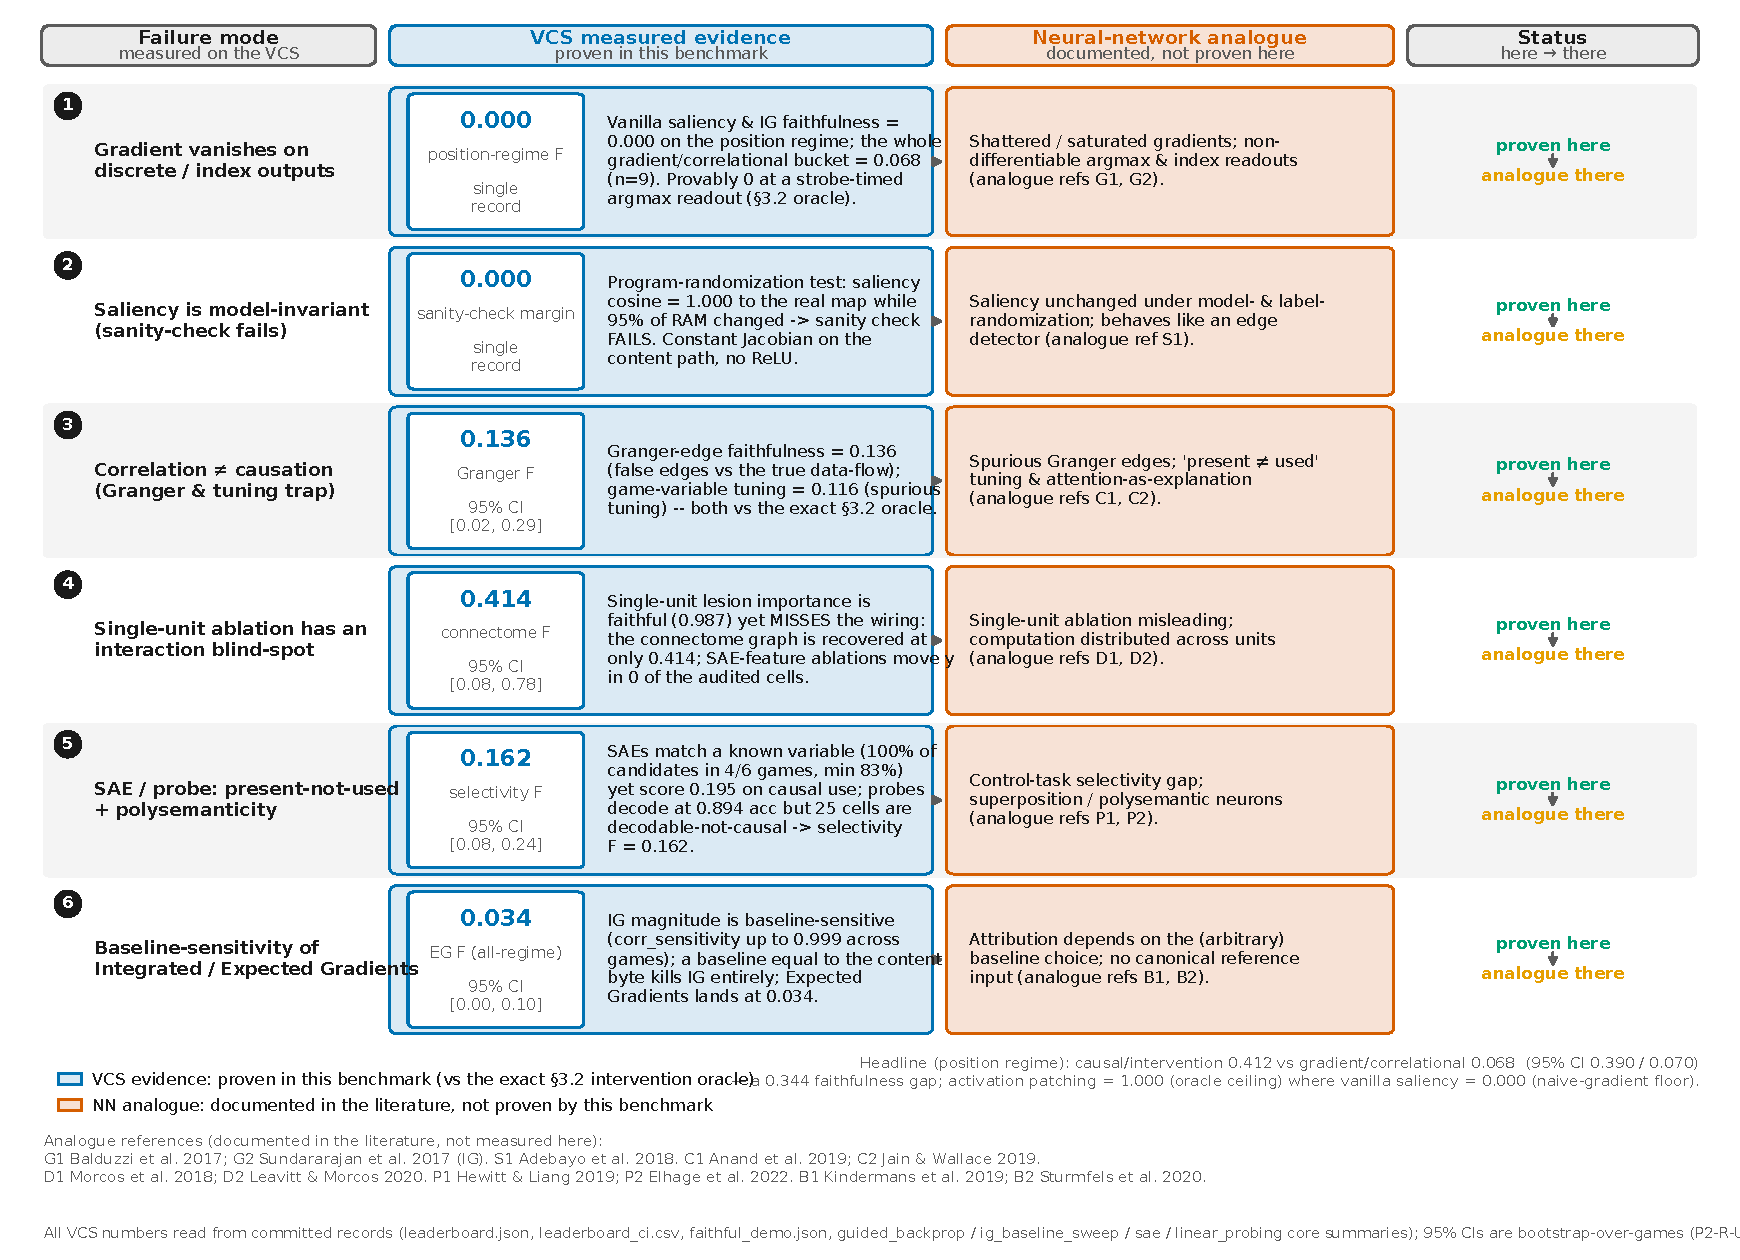
\includegraphics[width=\textwidth]{../figures/fig5_representativeness_map_full.pdf}
\caption{\textbf{Full VCS-to-NN representativeness map.} The full-density version of the
main-text map (Fig.~\ref{fig:representativeness}): each VCS failure mode is placed against its documented
neural-network analogue from the literature. The neural-network column records documented
analogues, not parallels proven by this benchmark; the oracle is the intervention oracle of
\Sectionname3.2, and the underlying per-method values trace to
\texttt{compare/out/leaderboard.json} via Sec.~\ref{supp:provenance}. Note that this full
map is the figure the simplified main-text version condenses.}
\label{supp:fig:repmap}
\end{figure}

\begin{figure}[t]
\centering
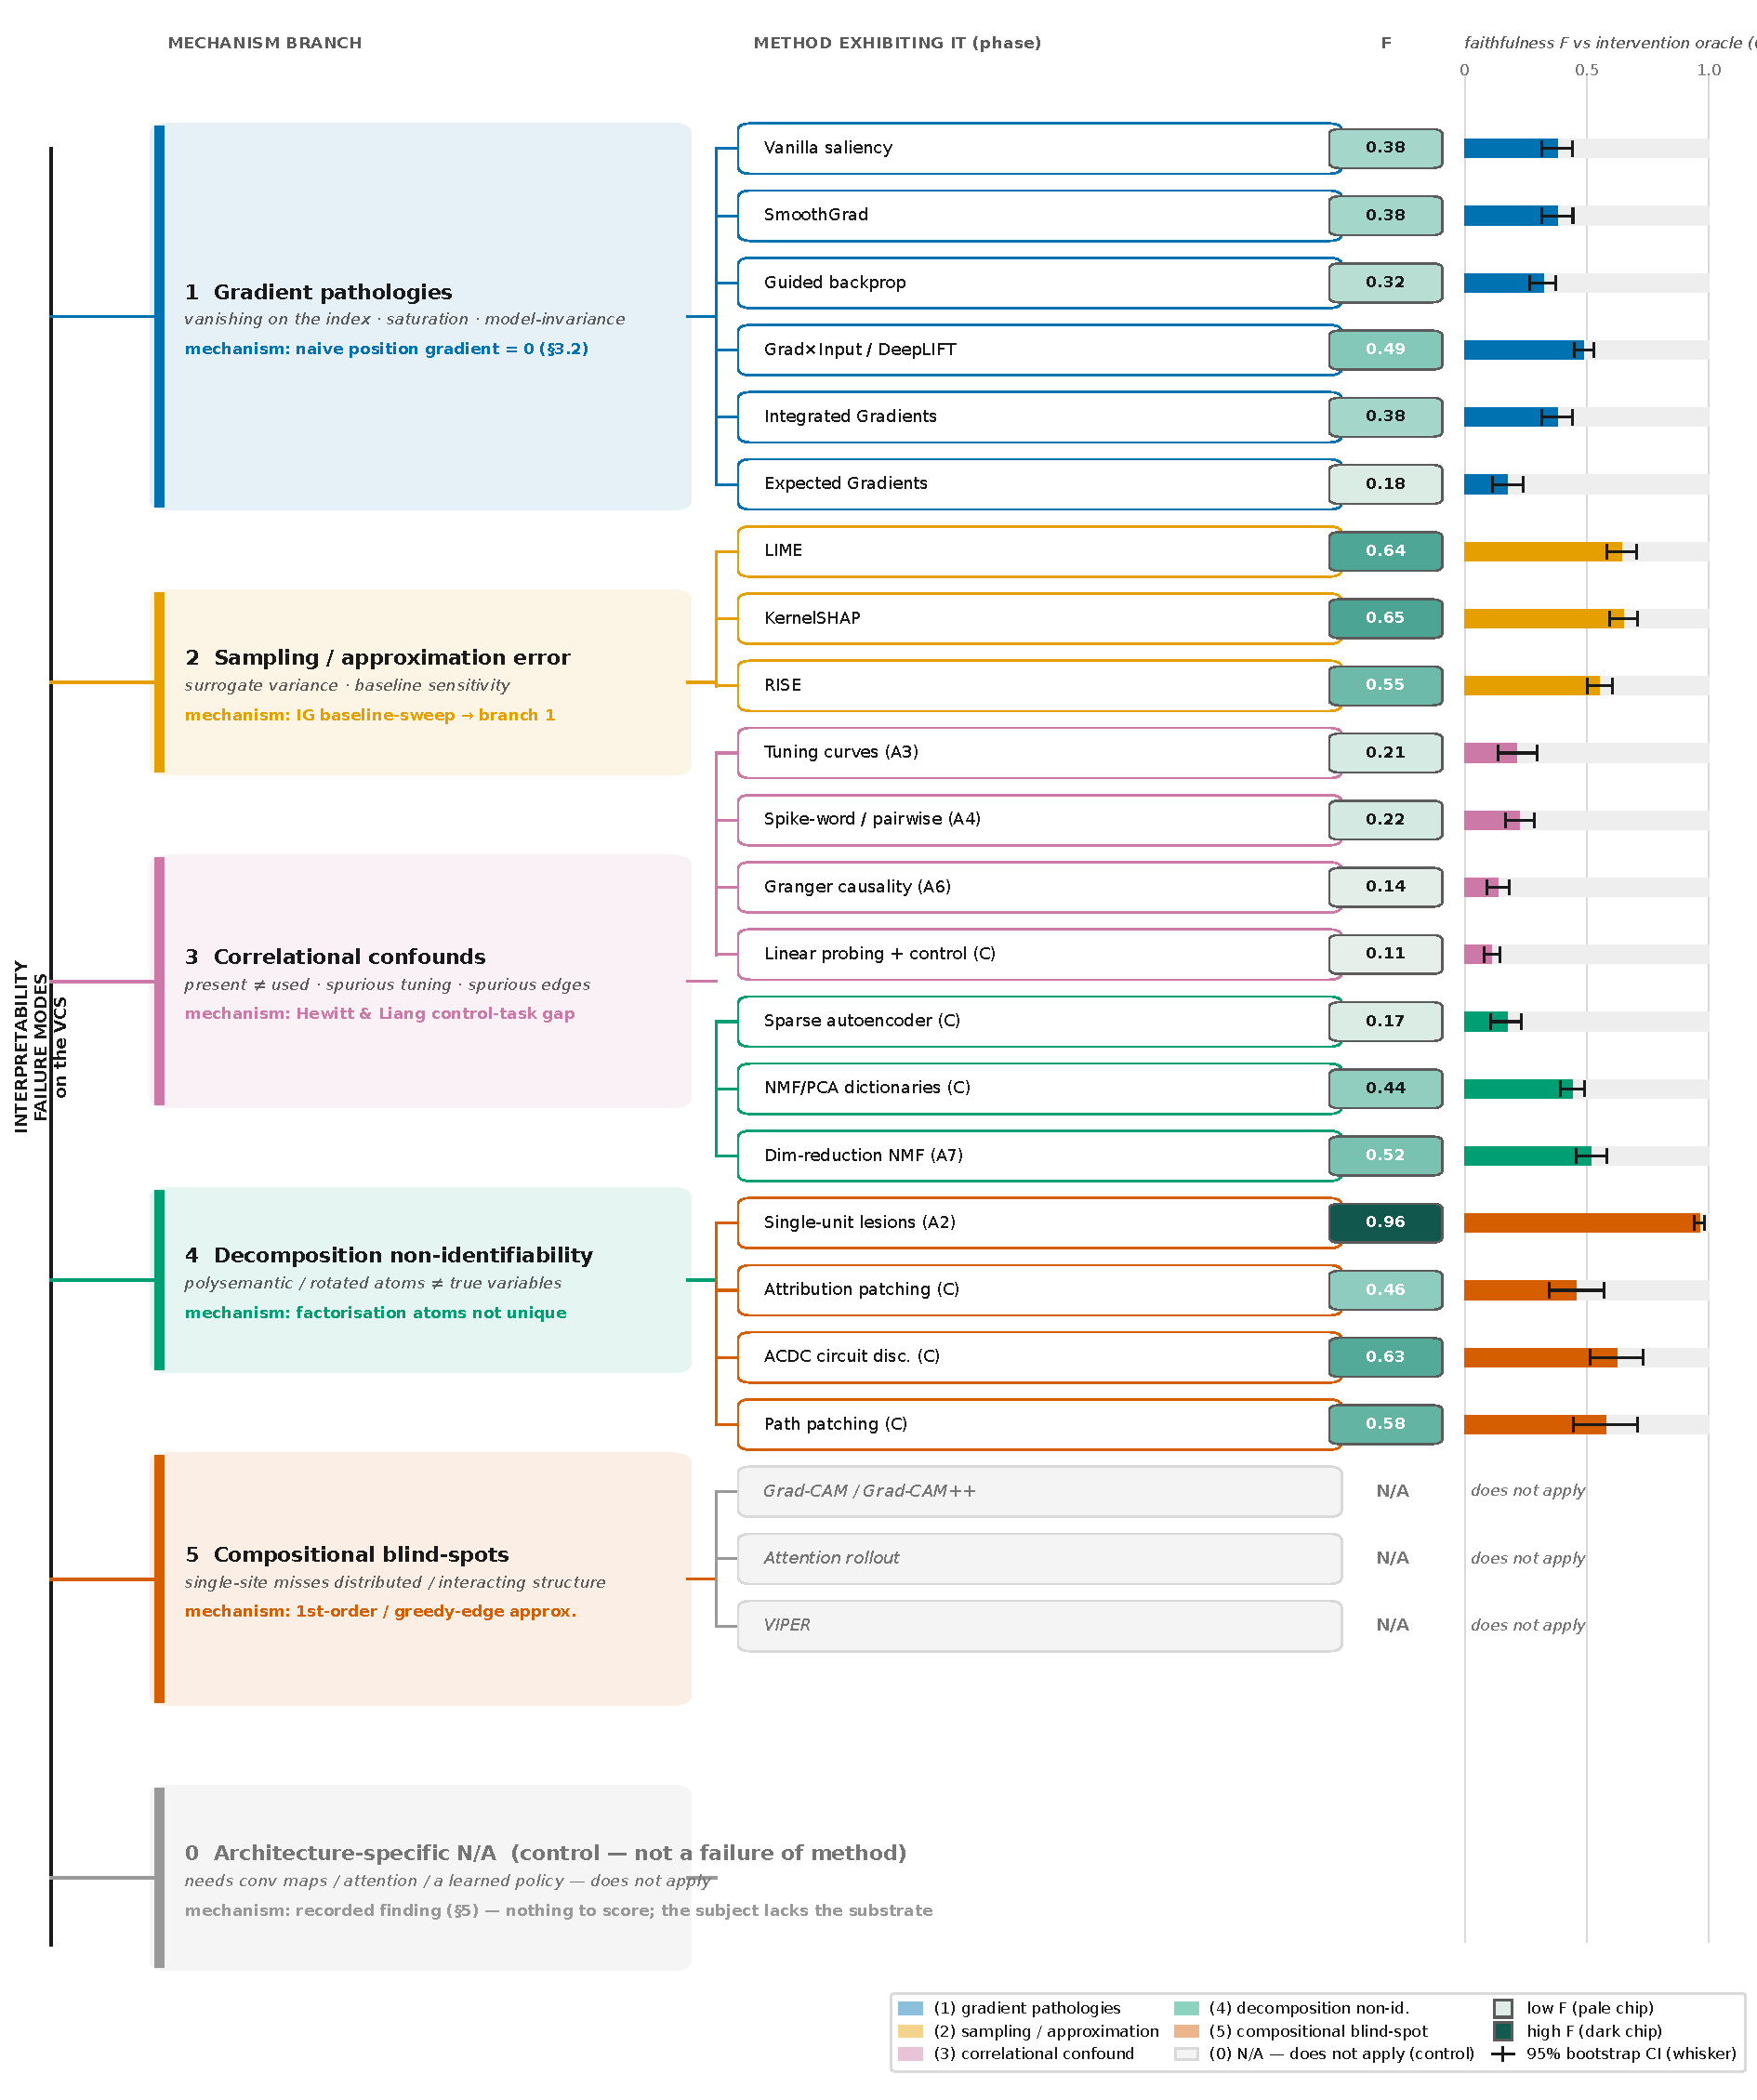
\includegraphics[width=\textwidth]{../figures/fig6_failure_taxonomy_full.pdf}
\caption{\textbf{Full failure taxonomy.} The full-density version of the main-text taxonomy
(Fig.~\ref{fig:taxonomy}): the families of interpretability failure observed on the machine, each annotated
with its faithfulness against the intervention oracle (\Sectionname3.2), reported as $F$ with its
$95\%$ bootstrap confidence interval. The leaf values trace to
\texttt{compare/out/leaderboard.json} and \texttt{leaderboard\_ci.csv} via
Sec.~\ref{supp:provenance}. Note that the gradient and correlational branches collapse on
the discrete position regime, where the naive gradient is provably zero (Prop.~\ref{prop:zero}).}
\label{supp:fig:taxonomy}
\end{figure}

\section{Plausibility-proxy rubric and its sensitivity}\label{supp:plausibility}

The plausibility axis of the leaderboard is a documented, tradition-level proxy, not a
human-subjects measurement. This section records how each value was assigned. It also shows
that the headline contrast does not depend on the particular numbers chosen. The Methods
(\Sectionname\ref{sec:triad}) name two reporting axes. Faithfulness is measured on the machine against the
intervention oracle of \Sectionname\ref{sec:oracle}. The plausibility proxy stands in for how convincing a
tradition's explanations are usually taken to be. We assign the proxy once per method
tradition, before any faithfulness score on our machine is computed, so it cannot be tuned to
the result. Its only job is to expose the danger zone of explanations that look convincing yet
are unfaithful. For that job it must be coarse, fixed in advance, and sourced rather than
precise.

The rubric assigns one proxy per tradition on a fixed five-step scale. It scores two
documented properties of each tradition's typical output and takes their average. The first
property is whether the explanation produces a dense, picture-like artifact that a reader sees
as an account of the computation. Heatmaps and saliency-style maps over the input are read as
convincing by construction. This is the perceptual-immediacy axis. The second property is
whether the field has historically treated the tradition's output as a self-evident
explanation rather than a hypothesis to be tested. This is the adoption-as-explanation axis. A
tradition that scores high on both, such as gradient saliency, receives a high proxy. A
tradition whose output is an austere intervention table or a circuit edge list, rarely
mistaken for a finished story, receives a low one. The scale is deliberately blunt,
$\{0.3,0.5,0.55,0.75,0.8,0.85,0.9\}$. A proxy meant to expose a danger zone gains nothing from
false precision, and a finer scale would invite over-reading. Every value in
Table~\ref{supp:tab:plausrubric} traces to the \jkey{plausibility_proxy} field of the
per-method rows in \texttt{compare/out/leaderboard.json}. The table only groups those rows by
tradition and records the rationale.

\begin{table}[t]
\centering
\caption{\textbf{Plausibility-proxy rubric.} The proxy assigned to each method tradition,
with the documented rationale. Values are the \jkey{plausibility_proxy} field of the
leaderboard rows (\texttt{compare/out/leaderboard.json}). They are tradition-level and fixed
before any faithfulness score is computed, so the proxy cannot be tuned to the measured
faithfulness. A higher value means an explanation that the field tends to find more
convincing, not one that is more faithful. The oracle (\Sectionname\ref{sec:oracle}) is the positive control and
is not a method under test.}
\label{supp:tab:plausrubric}
\begin{tabular}{@{}llp{6.4cm}@{}}
\toprule
Tradition & Proxy & Rationale (documented basis) \\
\midrule
gradient        & $0.90$ & Dense input-space heatmaps read as a visual account of the
                            decision; the most widely adopted XAI outputs, routinely shown
                            as if self-explanatory. \\
probing         & $0.85$ & A trained decoder that ``finds'' a concept reads as evidence the
                            concept is used; high adoption, though decodability is not
                            causal use. \\
correlational   & $0.80$ & Tuning curves and coupling spectra match the neuroscience idiom
                            of a convincing single-unit account. \\
dim.\ reduction & $0.75$ & Low-dimensional factors and dictionary atoms look like a clean
                            summary of the representation. \\
intervention    & $0.55$ & Occlusion and counterfactual outputs are quantitative tables, less
                            immediately picture-like, treated as tests rather than stories. \\
causal          & $0.50$ & Circuit edge lists and patching results are austere artifacts
                            rarely mistaken for a finished narrative. \\
descriptive     & $0.30$ & Whole-state recording is an explicit non-explanation: it withholds
                            nothing and reads as a dump, not an account. \\
\midrule
oracle (control)& $1.00$ & The \Sectionname\ref{sec:oracle} ground truth by construction; positive control, not a
                            method under test. \\
\bottomrule
\end{tabular}
\end{table}

The paper draws a contrast between this proxy and measured faithfulness. On the committed
records the two move in opposite directions. Across the thirty methods under test the Spearman
rank correlation between faithfulness and the proxy is $-0.36$, a negative association.
The traditions the field finds most convincing are, on this machine, among the least faithful.
Eight methods fall in the danger zone, defined here as a proxy of at least $0.70$ together
with a faithfulness below $0.40$. They include the correlational neuroscience methods, Expected
Gradients, guided backprop, linear probing, and the sparse autoencoder. The per-method extreme
makes the point sharply. Vanilla saliency has the highest proxy, $0.9$, yet scores faithfulness
$0.115$ on the position regime. Activation patching has a lower proxy, $0.5$, and scores $1.0$.
Here the less faithful method is the more plausible one. These figures are produced by
\texttt{tools/xai\_study/compare/plausibility\_sensitivity.py} from the leaderboard and
recorded in \texttt{compare/out/plausibility\_sensitivity.csv}.

A proxy fixed by a coarse rubric raises the question of whether the contrast is an artifact of
the particular numbers. The answer is that it is not. We perturb the proxy under four
deterministic schemes and recompute the relationship each time. The analysis uses fixed,
index-keyed offsets rather than random draws, so it re-derives bit-for-bit. The first scheme
adds a fixed per-method jitter of magnitude $\sigma\in\{0.05,0.1,0.2\}$, alternating in sign by
row. The second compresses every proxy toward the common mean by a fraction $\sigma$, which
preserves the rank order of traditions. The third uses the same index-keyed offsets at
$\sigma\in\{0.1,0.2\}$, large enough to swap neighbouring traditions' ranks. The fourth drops
one whole tradition at a time and recomputes on the remainder. Across all fourteen
perturbations the rank correlation between faithfulness and proxy stays negative. It ranges
from $-0.76$ to $-0.08$. The danger zone stays populated, with
between four and ten methods. The per-method anchor sign holds in every scheme where both
anchor methods are present, the more plausible saliency remaining the less faithful. Two runs
bound the range. The strongest is the leave-the-gradient-tradition-out run. It removes the most
plausible and least faithful block at once, and still leaves six danger-zone methods and a rank
correlation of $-0.76$. The weakest is the leave-the-causal-tradition-out run, where the
correlation falls to $-0.08$, close to zero; removing the faithful causal block flattens the
association, so the contrast is carried in part by that block. Table~\ref{supp:tab:plaussens}
reports the full sweep. The contrast keeps its sign under every alternative proxy assignment we
tried: plausibility and faithfulness are not the same axis, and high plausibility is no
guarantee of faithfulness.

\begin{table}[t]
\centering
\caption{\textbf{Proxy-sensitivity sweep.} The faithfulness-versus-proxy relationship under
each perturbation, from \texttt{compare/out/plausibility\_sensitivity.csv}. ``$\rho$'' is the
Spearman rank correlation between faithfulness and proxy over the methods present. ``danger''
is the count of high-proxy ($\geq0.70$), low-faithfulness ($<0.40$) methods. ``anchor'' is
$1$ when the more plausible saliency is the less faithful of the saliency/activation-patching
pair, and blank where a leave-one-out run removes an anchor. The baseline rubric is the first
row. Across every scheme the correlation stays negative and the danger zone stays populated.}
\label{supp:tab:plaussens}
\begin{tabular}{@{}llrrrc@{}}
\toprule
Scheme & Param & $n$ & $\rho$ & Danger & Anchor \\
\midrule
baseline                & ---           & 30 & $-0.36$ &  8 & 1 \\
additive jitter         & $\sigma=0.05$ & 30 & $-0.40$ &  8 & 1 \\
additive jitter         & $\sigma=0.10$ & 30 & $-0.41$ &  8 & 1 \\
additive jitter         & $\sigma=0.20$ & 30 & $-0.42$ & 10 & 1 \\
rank-preserving         & $\sigma=0.10$ & 30 & $-0.36$ &  8 & 1 \\
rank-preserving         & $\sigma=0.20$ & 30 & $-0.36$ &  8 & 1 \\
rank-jittering          & $\sigma=0.10$ & 30 & $-0.41$ &  8 & 1 \\
rank-jittering          & $\sigma=0.20$ & 30 & $-0.42$ & 10 & 1 \\
leave-out causal        & ---           & 24 & $-0.08$ &  8 & \\
leave-out correlational & ---           & 26 & $-0.40$ &  4 & 1 \\
leave-out descriptive   & ---           & 29 & $-0.29$ &  8 & 1 \\
leave-out dim.\ red.    & ---           & 27 & $-0.34$ &  7 & 1 \\
leave-out gradient      & ---           & 20 & $-0.76$ &  6 & \\
leave-out intervention  & ---           & 25 & $-0.34$ &  8 & 1 \\
leave-out probing       & ---           & 29 & $-0.36$ &  7 & 1 \\
\bottomrule
\end{tabular}
\end{table}

 into main.tex). It is also
%% a self-contained \input target: the six S-files below carry all SI content the main
%% paper promises (improvement_instructions P0#2, P0#4; P1#13, P1#14, P1#21; P3#35, P3#36).
%%
%% It re-uses, but does not re-derive, the §3 F/S/M definitions (S03 is authoritative)
%% and the canonical method count "30 interpretability methods + the oracle positive
%% control = 31 rows" (S07 is authoritative). Every reported number traces to a committed
%% record under tools/xai_study/compare/out/ (verifiable via the §6.5 traceability table
%% of REPRODUCIBILITY.md and re-derived by S5 below).
%%
%% Standalone compile (for review, before R6 wires it into main): wrap this file in the
%% sn-jnl preamble of a scratch driver (\documentclass[sn-nature,pdflatex]{sn-jnl} +
%% graphicx, booktabs, multirow, amsmath, longtable) and %% supplement.tex — Supplementary Information for Paper 2 (xai_2_interpretability).
%%
%% SCRUM note (P2-R-SUPP): this fragment is \input{} into the main paper by the SM
%% integration write (R6 wires %% supplement.tex — Supplementary Information for Paper 2 (xai_2_interpretability).
%%
%% SCRUM note (P2-R-SUPP): this fragment is \input{} into the main paper by the SM
%% integration write (R6 wires \input{supplement/supplement} into main.tex). It is also
%% a self-contained \input target: the six S-files below carry all SI content the main
%% paper promises (improvement_instructions P0#2, P0#4; P1#13, P1#14, P1#21; P3#35, P3#36).
%%
%% It re-uses, but does not re-derive, the §3 F/S/M definitions (S03 is authoritative)
%% and the canonical method count "30 interpretability methods + the oracle positive
%% control = 31 rows" (S07 is authoritative). Every reported number traces to a committed
%% record under tools/xai_study/compare/out/ (verifiable via the §6.5 traceability table
%% of REPRODUCIBILITY.md and re-derived by S5 below).
%%
%% Standalone compile (for review, before R6 wires it into main): wrap this file in the
%% sn-jnl preamble of a scratch driver (\documentclass[sn-nature,pdflatex]{sn-jnl} +
%% graphicx, booktabs, multirow, amsmath, longtable) and \input{supplement}; the tables
%% render without overfull boxes and the two SI figures resolve from ../figures/.

\clearpage
\appendix

%% Breakable monospaced JSON key: lets long under_scored keys wrap inside narrow table
%% columns. Used by S5 (number provenance). Defined here so the S-files stay self-contained.
\providecommand{\jkey}[1]{\texttt{\expandafter\jkeyaux#1\relax}}
\makeatletter
\def\jkeyaux#1{\ifx\relax#1\else
  \ifx_#1\discretionary{}{}{}\char`\_\else
    \ifx.#1\discretionary{}{}{}.\else#1\fi\fi
  \expandafter\jkeyaux\fi}
\makeatother

\section*{Supplementary Information}
\setcounter{table}{0}
\setcounter{figure}{0}
\renewcommand{\thetable}{S\arabic{table}}
\renewcommand{\thefigure}{S\arabic{figure}}
\renewcommand{\thesection}{S\arabic{section}}
\setcounter{section}{0}

This Supplementary Information records what the main paper summarizes. We give the
per-method protocols (\Sectionname\ref{supp:protocols}) and the leaderboard schema with its glossary
(\Sectionname\ref{supp:schema}). We give the coverage and applicability of every method across games
and output regimes (\Sectionname\ref{supp:coverage}). We map each headline claim to its evidence
(\Sectionname\ref{supp:claims}). We trace the provenance of every headline number down to the record
file and command that produced it (\Sectionname\ref{supp:provenance}). We state plainly what the
paper does not claim (\Sectionname\ref{supp:notclaimed}). We give the plausibility-proxy rubric and
its sensitivity analysis (\Sectionname\ref{supp:plausibility}). The main text shows simplified forms
of two diagnostic figures; we reproduce both here at full resolution
(Figs.~\ref{supp:fig:repmap} and~\ref{supp:fig:taxonomy}).
The correctness triad $\mathrm{F}\wedge\mathrm{S}\wedge\mathrm{M}$ used throughout is the
one defined in the main Methods (\Sectionname\ref{sec:triad}); we reference it here rather than restating it. The
benchmark scores 30 interpretability methods together with the intervention oracle (\Sectionname\ref{sec:oracle})
as a positive control, for 31 leaderboard rows in total.

\input{supplement/S1_per_method_protocols}
\input{supplement/S2_benchmark_schema}
\input{supplement/S3_coverage_applicability}
\input{supplement/S4_claims_evidence}
\input{supplement/S5_number_provenance}
\input{supplement/S6_not_claimed}
\input{supplement/S7_plausibility}
 into main.tex). It is also
%% a self-contained \input target: the six S-files below carry all SI content the main
%% paper promises (improvement_instructions P0#2, P0#4; P1#13, P1#14, P1#21; P3#35, P3#36).
%%
%% It re-uses, but does not re-derive, the §3 F/S/M definitions (S03 is authoritative)
%% and the canonical method count "30 interpretability methods + the oracle positive
%% control = 31 rows" (S07 is authoritative). Every reported number traces to a committed
%% record under tools/xai_study/compare/out/ (verifiable via the §6.5 traceability table
%% of REPRODUCIBILITY.md and re-derived by S5 below).
%%
%% Standalone compile (for review, before R6 wires it into main): wrap this file in the
%% sn-jnl preamble of a scratch driver (\documentclass[sn-nature,pdflatex]{sn-jnl} +
%% graphicx, booktabs, multirow, amsmath, longtable) and %% supplement.tex — Supplementary Information for Paper 2 (xai_2_interpretability).
%%
%% SCRUM note (P2-R-SUPP): this fragment is \input{} into the main paper by the SM
%% integration write (R6 wires \input{supplement/supplement} into main.tex). It is also
%% a self-contained \input target: the six S-files below carry all SI content the main
%% paper promises (improvement_instructions P0#2, P0#4; P1#13, P1#14, P1#21; P3#35, P3#36).
%%
%% It re-uses, but does not re-derive, the §3 F/S/M definitions (S03 is authoritative)
%% and the canonical method count "30 interpretability methods + the oracle positive
%% control = 31 rows" (S07 is authoritative). Every reported number traces to a committed
%% record under tools/xai_study/compare/out/ (verifiable via the §6.5 traceability table
%% of REPRODUCIBILITY.md and re-derived by S5 below).
%%
%% Standalone compile (for review, before R6 wires it into main): wrap this file in the
%% sn-jnl preamble of a scratch driver (\documentclass[sn-nature,pdflatex]{sn-jnl} +
%% graphicx, booktabs, multirow, amsmath, longtable) and \input{supplement}; the tables
%% render without overfull boxes and the two SI figures resolve from ../figures/.

\clearpage
\appendix

%% Breakable monospaced JSON key: lets long under_scored keys wrap inside narrow table
%% columns. Used by S5 (number provenance). Defined here so the S-files stay self-contained.
\providecommand{\jkey}[1]{\texttt{\expandafter\jkeyaux#1\relax}}
\makeatletter
\def\jkeyaux#1{\ifx\relax#1\else
  \ifx_#1\discretionary{}{}{}\char`\_\else
    \ifx.#1\discretionary{}{}{}.\else#1\fi\fi
  \expandafter\jkeyaux\fi}
\makeatother

\section*{Supplementary Information}
\setcounter{table}{0}
\setcounter{figure}{0}
\renewcommand{\thetable}{S\arabic{table}}
\renewcommand{\thefigure}{S\arabic{figure}}
\renewcommand{\thesection}{S\arabic{section}}
\setcounter{section}{0}

This Supplementary Information records what the main paper summarizes. We give the
per-method protocols (\Sectionname\ref{supp:protocols}) and the leaderboard schema with its glossary
(\Sectionname\ref{supp:schema}). We give the coverage and applicability of every method across games
and output regimes (\Sectionname\ref{supp:coverage}). We map each headline claim to its evidence
(\Sectionname\ref{supp:claims}). We trace the provenance of every headline number down to the record
file and command that produced it (\Sectionname\ref{supp:provenance}). We state plainly what the
paper does not claim (\Sectionname\ref{supp:notclaimed}). We give the plausibility-proxy rubric and
its sensitivity analysis (\Sectionname\ref{supp:plausibility}). The main text shows simplified forms
of two diagnostic figures; we reproduce both here at full resolution
(Figs.~\ref{supp:fig:repmap} and~\ref{supp:fig:taxonomy}).
The correctness triad $\mathrm{F}\wedge\mathrm{S}\wedge\mathrm{M}$ used throughout is the
one defined in the main Methods (\Sectionname\ref{sec:triad}); we reference it here rather than restating it. The
benchmark scores 30 interpretability methods together with the intervention oracle (\Sectionname\ref{sec:oracle})
as a positive control, for 31 leaderboard rows in total.

\input{supplement/S1_per_method_protocols}
\input{supplement/S2_benchmark_schema}
\input{supplement/S3_coverage_applicability}
\input{supplement/S4_claims_evidence}
\input{supplement/S5_number_provenance}
\input{supplement/S6_not_claimed}
\input{supplement/S7_plausibility}
; the tables
%% render without overfull boxes and the two SI figures resolve from ../figures/.

\clearpage
\appendix

%% Breakable monospaced JSON key: lets long under_scored keys wrap inside narrow table
%% columns. Used by S5 (number provenance). Defined here so the S-files stay self-contained.
\providecommand{\jkey}[1]{\texttt{\expandafter\jkeyaux#1\relax}}
\makeatletter
\def\jkeyaux#1{\ifx\relax#1\else
  \ifx_#1\discretionary{}{}{}\char`\_\else
    \ifx.#1\discretionary{}{}{}.\else#1\fi\fi
  \expandafter\jkeyaux\fi}
\makeatother

\section*{Supplementary Information}
\setcounter{table}{0}
\setcounter{figure}{0}
\renewcommand{\thetable}{S\arabic{table}}
\renewcommand{\thefigure}{S\arabic{figure}}
\renewcommand{\thesection}{S\arabic{section}}
\setcounter{section}{0}

This Supplementary Information records what the main paper summarizes. We give the
per-method protocols (\Sectionname\ref{supp:protocols}) and the leaderboard schema with its glossary
(\Sectionname\ref{supp:schema}). We give the coverage and applicability of every method across games
and output regimes (\Sectionname\ref{supp:coverage}). We map each headline claim to its evidence
(\Sectionname\ref{supp:claims}). We trace the provenance of every headline number down to the record
file and command that produced it (\Sectionname\ref{supp:provenance}). We state plainly what the
paper does not claim (\Sectionname\ref{supp:notclaimed}). We give the plausibility-proxy rubric and
its sensitivity analysis (\Sectionname\ref{supp:plausibility}). The main text shows simplified forms
of two diagnostic figures; we reproduce both here at full resolution
(Figs.~\ref{supp:fig:repmap} and~\ref{supp:fig:taxonomy}).
The correctness triad $\mathrm{F}\wedge\mathrm{S}\wedge\mathrm{M}$ used throughout is the
one defined in the main Methods (\Sectionname\ref{sec:triad}); we reference it here rather than restating it. The
benchmark scores 30 interpretability methods together with the intervention oracle (\Sectionname\ref{sec:oracle})
as a positive control, for 31 leaderboard rows in total.

\section{Per-method protocols}\label{supp:protocols}

This section records five things for each method under test. It records the exact objects the
method consumes and produces, the reference it is scored against, its sampling or optimization
budget, the metric that turns its output into a faithfulness score, and the committed record
file (version-controlled, in the released repository) that holds the per-game results. All methods share one evaluation contract. We state that
contract once and then specialize it per method. Every method receives the same bit-exact VCS
state on each game of the scored set. We state the contract on the six core games
(\texttt{breakout}, \texttt{ms\_pacman}, \texttt{pong}, \texttt{qbert}, \texttt{seaquest},
\texttt{space\_invaders}), which carry the full tiered ground truth and the exact oracle and
serve as the running example; the aggregate leaderboard scores extend the identical protocol
to the 42-game scored set of \Sectionname\ref{supp:scoredset}. That state is not the boot screen.
It is a shared gameplay state, produced by a single seeded random-action stream (seed~$0$) run
for a $90$-frame prefix and then rolled forward for a $15$-frame analysis horizon. The stream is
deterministic, so every method sees the identical state on each game, and the run is asserted
bit-exact per game. An oracle cause-density gate screens the state before any method runs. The
gate counts how many candidate causes move the output above a floor and rejects states with too
few, so a near-flat oracle column cannot pass. This gate is what turns a degenerate frame into a
usable one; on \texttt{seaquest} it raises the count of live candidate causes from $2$ to $19$.
The candidate-cause set is the machine's own state. This set is the RAM bytes together with the
CPU registers and the TIA and RIOT registers exposed by the substrate. The output every method
attributes over is a shared screen-buffer region read at the end of the analysis horizon, not a
single hand-picked pixel. The reference is the intervention oracle of \Sectionname\ref{sec:oracle},
evaluated by exact re-runs of the emulator under $\mathrm{do}(u)$. A method that
cannot be applied to a given output regime is recorded as not-applicable rather than scored
as zero. An empty result is therefore never read as a wrong one. Faithfulness is the F
axis of the main-text triad (\Sectionname\ref{sec:triad}); we reference that definition and do not restate it.
Records live under \texttt{tools/xai\_study/<phase>/out/}; the aggregate they feed is
\texttt{tools/xai\_study/compare/out/leaderboard.json}.
Table~\ref{supp:leaderboard} consolidates the triad scores for all thirty methods and the
oracle positive control in one place; the per-method protocols follow.

\begin{table*}[t]
\centering
\caption{\textbf{Consolidated leaderboard: all methods, all triad axes.} One row per method
across the three phases, plus the intervention oracle as a positive control. $F$ is
faithfulness (Pearson correlation against the oracle, with the bootstrap-over-games 95\% CI in
brackets), $S$ is sufficiency, $M$ is minimality, all as defined in \Sectionname\ref{sec:triad};
Plaus is the elicited plausibility prior and $n$ is the number of scored games. Attribution
methods that emit only a saliency have no defined $S$ or $M$ and are marked ``---''; A5
(field potentials) and A7 (dimensionality reduction) likewise lack the $S$/$M$ decomposition.
Values are transcribed from \texttt{tools/xai\_study/compare/out/leaderboard.json} (the
committed numbers of record).}
\label{supp:leaderboard}
\footnotesize
\setlength{\tabcolsep}{4pt}
\begin{tabularx}{\textwidth}{@{}Xccccccc@{}}
\toprule
Method & Phase & Tradition & $F$ (95\% CI) & $S$ & $M$ & Plaus & $n$ \\
\midrule
A1 connectomics & A & intervention & 0.207 [0.130, 0.293] & 0.971 & 0.967 & 0.55 & 35 \\
A2 lesions & A & intervention & 0.965 [0.942, 0.983] & 0.591 & 1.000 & 0.55 & 42 \\
A3 tuning curves & A & correlational & 0.213 [0.136, 0.295] & 0.200 & 0.928 & 0.80 & 42 \\
A4 spike-word / pairwise & A & correlational & 0.225 [0.166, 0.283] & 0.133 & 0.363 & 0.80 & 34 \\
A5 field potentials & A & correlational & 0.376 [0.323, 0.428] & --- & --- & 0.80 & 40 \\
A6 Granger & A & correlational & 0.136 [0.091, 0.184] & 0.884 & 0.647 & 0.80 & 35 \\
A7 dim.\ reduction & A & dim.\ red. & 0.519 [0.457, 0.581] & --- & --- & 0.75 & 42 \\
A8 whole-state & A & descriptive & 1.000 [1.000, 1.000] & 1.000 & 0.075 & 0.30 & 42 \\
\midrule
Vanilla saliency & B & gradient & 0.380 [0.316, 0.445] & --- & --- & 0.90 & 42 \\
smoothgrad & B & gradient & 0.380 [0.317, 0.445] & --- & --- & 0.90 & 42 \\
Guided backprop & B & gradient & 0.322 [0.267, 0.375] & --- & --- & 0.90 & 42 \\
Grad$\times$Input / DeepLIFT & B & gradient & 0.486 [0.448, 0.526] & --- & --- & 0.90 & 42 \\
Integrated Gradients & B & gradient & 0.379 [0.314, 0.444] & --- & --- & 0.90 & 42 \\
Expected Gradients & B & gradient & 0.175 [0.110, 0.240] & --- & --- & 0.90 & 42 \\
kernelshap & B & gradient & 0.652 [0.596, 0.709] & --- & --- & 0.90 & 42 \\
lime & B & gradient & 0.644 [0.582, 0.705] & --- & --- & 0.90 & 42 \\
rise & B & gradient & 0.552 [0.500, 0.600] & --- & --- & 0.90 & 42 \\
occlusion & B & intervention & 0.687 [0.624, 0.746] & --- & --- & 0.55 & 42 \\
Extremal perturbation & B & intervention & 0.461 [0.410, 0.513] & --- & --- & 0.55 & 42 \\
On-distribution counterfactual & B & intervention & 0.433 [0.343, 0.522] & --- & --- & 0.55 & 42 \\
\midrule
Activation patching & C & causal & 1.000 [1.000, 1.000] & --- & --- & 0.50 & 42 \\
Causal scrubbing & C & causal & 0.979 [0.940, 1.000] & 0.979 & 0.814 & 0.50 & 42 \\
Interchange interventions (DAS) & C & causal & 1.000 [1.000, 1.000] & --- & --- & 0.50 & 42 \\
Logit / tuned lens & C & causal & 0.820 [0.768, 0.871] & --- & 0.224 & 0.50 & 42 \\
Path patching & C & causal & 0.580 [0.452, 0.710] & --- & --- & 0.50 & 42 \\
ACDC & C & causal & 0.625 [0.514, 0.730] & 0.299 & 1.000 & 0.50 & 35 \\
Attribution patching & C & gradient & 0.456 [0.345, 0.573] & --- & --- & 0.90 & 42 \\
Linear probing (+ control) & C & probing & 0.240 [0.153, 0.346] & --- & 0.932 & 0.85 & 42 \\
NMF / PCA dictionaries & C & dim.\ red. & 0.102 [0.049, 0.160] & 0.751 & 0.966 & 0.75 & 42 \\
Sparse autoencoder & C & dim.\ red. & 0.153 [0.096, 0.218] & 0.183 & 0.934 & 0.75 & 40 \\
\midrule
Intervention oracle & --- & oracle & 1.000 [1.000, 1.000] & 1.000 & 1.000 & 1.00 & 1 \\
\bottomrule
\end{tabularx}
\end{table*}

The neuroscience analyses (Phase~A) treat the running machine as a brain. It asks how far
each classical analysis recovers the known mechanism on the shared gameplay state. Each
method's baseline is the exact data-flow graph or causal role that the substrate makes
available. Its budget is the scored set (\Sectionname\ref{supp:scoredset}) unless noted,
with the six-game core as the running example, and its scoring metric is named in
Table~\ref{supp:tab:phaseA}. One core cell is honestly degenerate. On \texttt{ms\_pacman} the
pairwise analysis (A4) finds no coupled candidate pair to score at that frame, so its
\texttt{ms\_pacman} value is uninformative rather than a failure; the other five games carry
it.

\begin{table}[t]
\centering
\caption{\textbf{Phase~A protocols (neuroscience analyses).} One row per method. The columns
give the input it reads, the reference it is scored against, the sampling or intervention
budget, the scoring metric, and the committed record. All eight run on the scored set
(\Sectionname\ref{supp:scoredset}), with the six core games as the running example;
faithfulness is the F axis of \Sectionname\ref{sec:triad}. The whole-state recording (A8) is included as a
descriptive upper bound on coverage. Its faithfulness $F$ is trivial, so we read it for its
minimality $M$.}
\label{supp:tab:phaseA}
\scriptsize
\setlength{\tabcolsep}{4pt}
\begin{tabular}{@{}p{1.7cm}p{2.6cm}p{1.9cm}p{2.6cm}p{1.0cm}@{}}
\toprule
Method & Input / candidate causes & Reference & Scoring metric & Record \\
\midrule
A1 connectomics & RAM/register activity over trajectory & data-flow graph & data-flow graph $F_1$ vs.\ oracle & A1 \\
A2 lesions & single-cell knockouts via $\mathrm{do}(u)$ & true causal role & lesion-importance $\rho$ vs.\ role & A2 \\
A3 tuning curves & per-cell response vs.\ variable & variable coupling & $1-$ spurious-tuning rate & A3 \\
A4 spike-word / pairwise & pairwise cell correlations & true coupling & corr.\ $\rho$ vs.\ coupling & A4 \\
A5 field potentials & pooled-activity spectra & true causal share & $1-$ clock-explained var. & A5 \\
A6 Granger & directed lag structure & true data-flow & $1-$ false-edge rate & A6 \\
A7 dim.\ reduction & NMF/PCA over activity & known variables & NMF matched-component frac. & A7 \\
A8 whole-state & full state record & oracle decomp. & minimality $M$ vs.\ oracle & A8 \\
\bottomrule
\end{tabular}

\smallskip
\noindent\scriptsize Records: \texttt{tools/xai\_study/phaseA\_kording/out/A\{1..8\}\_*}; all
eight run on the 42-game scored set (\Sectionname\ref{supp:scoredset}), with the six core
games as the running example (\jkey{n_games} per method in \jkey{leaderboard.json}).
\end{table}

The attribution methods (Phase~B) run the everyday XAI toolbox over the same gameplay state.
These methods produce a real-valued saliency or attribution over the candidate-cause set.
We score that output by Pearson correlation against the oracle attribution. The gradient family
runs with the bilinear sub-pixel sampler turned on, so it is scored on a real position gradient
and not on the naive one. The naive gradient of the discrete position output is provably zero
(Prop.~\ref{prop:zero}); the sampler restores a finite gradient, but the restored gradient is
low and mixed in faithfulness rather than a fix. Expected Gradients draws its reference pool
from the states of the same seeded gameplay trajectory, not from a synthetic baseline. Two cells
are honestly degenerate and recorded as such. The on-distribution counterfactual returns a zero
delta on \texttt{space\_invaders}, \texttt{ms\_pacman}, and \texttt{qbert}, where its perturbation
does not move the shared output at that frame; those cells are marked not-valid rather than
scored. Expected Gradients scores low on the content regime of every game except \texttt{pong},
because the causal byte it should land on is static there. The budgets that matter are the
Monte-Carlo or perturbation counts of the sampling estimators, recorded per method in
Table~\ref{supp:tab:phaseB}. The seed-dispersion of the stochastic members is carried in
\texttt{leaderboard\_ci.csv} (\texttt{seed\_sd}, \texttt{seed\_sd\_source}) and reproduced
in \Sectionname\ref{supp:provenance}.

\begin{table}[t]
\centering
\caption{\textbf{Phase~B protocols (attribution methods).} Each method emits a saliency over
the candidate-cause set. We score it by Pearson correlation against the oracle attribution
(\Sectionname\ref{sec:oracle}). The reference is shared and the budget is the scored set of
\Sectionname\ref{supp:scoredset} (six core games as the running example). The budget column records the
sampling or perturbation count that drives each estimator. The seed column flags which
methods carry an independent-seed dispersion in \texttt{leaderboard\_ci.csv}.}
\label{supp:tab:phaseB}
\scriptsize
\setlength{\tabcolsep}{4pt}
\begin{tabular}{@{}p{2.9cm}p{1.75cm}p{4.3cm}p{1.15cm}@{}}
\toprule
Method & Tradition & Budget / hyperparameters & Seed sd \\
\midrule
Vanilla saliency & gradient & single backward pass & --- \\
smoothgrad & gradient & noise-averaged gradient; $\sigma$-robustness committed & 0.0 \\
Guided backprop & gradient & single guided pass & --- \\
Grad$\times$Input / DeepLIFT & gradient & DeepLIFT reference-difference & --- \\
Integrated Gradients & gradient & path integral, baseline = zero state & --- \\
Expected Gradients & gradient & expectation over baselines (refits) & yes \\
kernelshap & gradient & Monte-Carlo coalition sampling ($\propto 1/\sqrt{N}$) & 0.017 \\
lime & gradient & local linear fit, perturbation refits & 0.029 \\
rise & gradient & random-mask Monte-Carlo ($\propto 1/\sqrt{N}$) & 0.051 \\
occlusion & intervention & exhaustive single-cell masking & --- \\
Extremal perturbation & intervention & optimized mask, area-constrained & --- \\
On-distribution counterfactual & intervention & on-manifold $\mathrm{do}(u)$ resampling & --- \\
\bottomrule
\end{tabular}

\smallskip
\noindent\scriptsize Records: \texttt{tools/xai\_study/phaseB\_attribution/out/}; all twelve run
on the 42-game scored set (\Sectionname\ref{supp:scoredset}), six core games as the running
example, and are scored by Pearson correlation against the oracle (\Sectionname\ref{sec:oracle}). Seed
sd is the independent-seed dispersion from \texttt{leaderboard\_ci.csv}.
\end{table}

The mechanistic methods (Phase~C) are built to recover circuits. Each is scored
against the true data-flow or the exact recovered-minus-exact deviation. The causal members
of this phase are the ones that reach the oracle ceiling. We list their exact scoring metric
so that the ceiling is not read as a tautology. Each member is scored against the substrate's
known routine, and not against another method. Two members (NMF/PCA dictionaries and the
sparse autoencoder) are dimensionality-reduction methods carried here for comparison. The
sparse autoencoder has two aggregations that differ, which we reconcile in
\Sectionname\ref{supp:provenance}.

\begin{table}[t]
\centering
\caption{\textbf{Phase~C protocols (mechanistic methods).} Each method is scored against the
substrate's known circuit or the exact recovered-minus-exact deviation (\Sectionname\ref{sec:oracle}), and not
against another method. This is what keeps the oracle ceiling non-circular. The probing and
dictionary-learning members are included for comparison with the causal members.}
\label{supp:tab:phaseC}
\scriptsize
\setlength{\tabcolsep}{4pt}
\begin{tabular}{@{}p{3.4cm}p{1.4cm}p{5.2cm}@{}}
\toprule
Method & Tradition & Scoring metric \\
\midrule
Activation patching & causal & $\max|\text{recovered}-\text{exact}|$ vs.\ oracle \\
Causal scrubbing & causal & scrubbing-preserved performance \\
Interchange interventions (DAS) & causal & aligned interchange accuracy \\
Logit / tuned lens & causal & logit-lens fidelity to true intermediate \\
Path patching & causal & path-circuit $F_1$ vs.\ true routine \\
ACDC & causal & discovered-circuit best $F_1$ vs.\ data-flow \\
Attribution patching & gradient & corr.\ of approximation vs.\ exact patch \\
Linear probing (+ control) & probing & selectivity vs.\ control task \\
NMF / PCA dictionaries & dim.\ red. & matched-component fraction vs.\ vars \\
Sparse autoencoder & dim.\ red. & feature-variable matched fraction \\
\bottomrule
\end{tabular}

\smallskip
\noindent\scriptsize Records: \texttt{tools/xai\_study/phaseC\_mechanistic/out/}; all ten run
on the 42-game scored set (\Sectionname\ref{supp:scoredset}), with the six core games as the
running example.
\end{table}

The intervention oracle is the positive control, not a method under test. It is the exact
$\mathrm{do}(u)$ ground truth of \Sectionname\ref{sec:oracle}, evaluated by re-running the bit-exact machine. It
attains $F=S=M=1.0$ by construction. Its record triple is the intervention oracle, the
content-path gradient oracle, and their cross-check
(\texttt{tools/xai\_study/ground\_truth/out/}). It anchors the ceiling against which every
other row is read, which is why it occupies the thirty-first leaderboard row.

\section{Benchmark schema and glossary}\label{supp:schema}

The leaderboard is built from a flat record schema. Stating it removes the ambiguity
about what a single number on the benchmark counts. Each method is run per game and writes a
per-game record under its phase's \texttt{out/} tree. The leaderboard aggregates those
records into one row per method by averaging over games. The schema columns of a leaderboard
row are given in Table~\ref{supp:tab:schema}. The aggregation rule is a mean over the
$n_{\text{games}}$ games. When a method emits several output records on one game, those records
are first reduced within that game. The faithfulness, sufficiency, and minimality columns
report the F, S, and M axes defined in \Sectionname\ref{sec:triad}. We do not re-derive those definitions here.

\begin{table}[t]
\centering
\caption{\textbf{Leaderboard row schema.} The columns of one row in
\texttt{compare/out/leaderboard.json} (\texttt{rows[\,]}) and its uncertainty companion
\texttt{leaderboard\_ci.csv}. The metric column names the per-method scoring function from
\Sectionname\ref{supp:protocols}; F, S, and M are the triad axes of \Sectionname\ref{sec:triad}. Aggregation is a mean
over $n_{\text{games}}$, with bootstrap confidence intervals over games (and, where present,
over records).}
\label{supp:tab:schema}
\footnotesize
\begin{tabular}{@{}p{3.0cm}p{8.4cm}@{}}
\toprule
Column & Meaning \\
\midrule
\texttt{phase} & phaseA\_kording, phaseB\_attribution, phaseC\_mechanistic, or ground\_truth \\
\texttt{method} & method identifier (the row key) \\
\texttt{tradition} & intervention, causal, gradient, correlational, \jkey{dim_reduction}, probing, descriptive, oracle \\
\jkey{n_games} & number of games the method was scored on (up to 42 for the scored set of \Sectionname\ref{supp:scoredset}; 1 for the oracle) \\
\jkey{n_records} & number of per-game output records aggregated into the row \\
\texttt{faithfulness} (F) & faithfulness vs.\ the intervention oracle (\Sectionname\ref{sec:oracle}), $[0,1]$, higher better \\
\jkey{faithfulness_ci95} & $95\%$ bootstrap CI half-width over games \\
\jkey{faithfulness_position_regime} & F restricted to the discrete sprite-position/index regime \\
\jkey{faithfulness_content_regime} & F restricted to the continuous content regime \\
\texttt{triad\_S} / \texttt{triad\_M} & sufficiency / minimality axes (\Sectionname\ref{sec:triad}), where applicable \\
\jkey{plausibility_proxy} & documented method-tradition proxy, $[0,1]$ --- not a human-subjects measurement \\
\jkey{is_positive_control} & 1 for the oracle row, 0 otherwise \\
\jkey{metric_names} & the per-method scoring function (\Sectionname\ref{supp:protocols}) \\
\texttt{commits} & the commit(s) at which the per-game records were produced \\
\bottomrule
\end{tabular}
\end{table}

We fix the vocabulary that the schema implies, because the review asked for a single
unambiguous method count. A \emph{method} is one interpretability technique, e.g.\
\texttt{vanilla\_saliency}. A \emph{method row} is its single aggregated line on the
leaderboard. A \emph{per-game record} is one method scored on one game, written under a phase
\texttt{out/} tree. An \emph{output record} is a per-game record for one output regime; a
method may emit several of these on one game. A \emph{family mean} is the average over the
members of a tradition family, e.g.\ causal/intervention. The \emph{oracle positive control}
is the exact $\mathrm{do}(u)$ ground truth of \Sectionname\ref{sec:oracle}, scored as a method to anchor the
ceiling. A \emph{not-applicable method} is one that does not apply to a given output regime;
it is recorded as N/A rather than as a zero. With this vocabulary the count is unambiguous.
The benchmark scores 30 interpretability methods together with the intervention
oracle as a positive control, for 31 leaderboard rows in total
(\texttt{leaderboard.json.n\_methods}~$=31$), aggregating 1773 per-game records over the
42-game scored set (\texttt{n\_per\_game\_records\_aggregated}~$=1773$): 8 methods in
Phase~A, 12 in Phase~B, 10 in Phase~C, and the one oracle row. This count is the canonical one
used in the abstract, the figures, and throughout this Supplement.

\section{Coverage and applicability}\label{supp:coverage}

The benchmark scores methods on a six-game core drawn from a larger bit-exact substrate. The
coverage table makes the scope of that choice explicit. Paper~1 validates the
differentiable VCS ports bit-for-bit against the \texttt{xitari} reference on all 64 Arcade
Learning Environment games, within a 30-frame RAM and 60-frame screen window. The
interpretability study reported here runs on the six games listed in
Table~\ref{supp:tab:coverage}. Every method is scored on a shared gameplay state, produced by
one seeded random-action stream (seed~$0$, $90$-frame prefix, $15$-frame analysis horizon), not
on the boot screen. This keeps the analysis inside the Paper~1 bit-exact window while giving the
oracle a rich, non-degenerate cause set to score against. We pick these six games because all
three tiers of ground truth (\Sectionname\ref{sec:tiers}) are available for them and the oracle is
exact. The remaining 58 games are
bit-exact substrate but are not scored here. Some fall outside the validated horizon for the
analyses we run. For others, the tiered labels they would need are not yet produced. They are
candidates for the larger sweep, and are not excluded for any methodological reason. The
horizon column records the validated window. The tier column records which of the three
ground-truth tiers (T1 exact intervention, T2 data-flow, T3 externally-supplied semantic
labels) is available.

\begin{table}[t]
\centering
\caption{\textbf{Core-game coverage.} The six core games carry exact tiered ground truth and
the full method battery. Faithfulness is scored within the Paper~1 bit-exact window. The
last two columns give the methods run and the per-game output records contributed. The wider
64-game substrate is bit-exact (Paper~1) but is reserved for the larger sweep. T3 labels are
external (\Sectionname\ref{sec:tiers}); we record this so the benchmark does not appear to certify them.}
\label{supp:tab:coverage}
\footnotesize
\setlength{\tabcolsep}{4pt}
\begin{tabular}{@{}p{2.4cm}p{1.9cm}p{1.5cm}p{1.7cm}p{1.5cm}p{1.4cm}@{}}
\toprule
Game & Paper-1 status & Horizon & Tiers & Methods run & Records \\
\midrule
breakout & bit-exact & 30/60 fr & T1,T2,T3 & 30 + oracle & per-game \\
ms\_pacman & bit-exact & 30/60 fr & T1,T2,T3 & 30 + oracle & per-game \\
pong & bit-exact & 30/60 fr & T1,T2,T3 & 30 + oracle & per-game \\
qbert & bit-exact & 30/60 fr & T1,T2,T3 & 30 + oracle & per-game \\
seaquest & bit-exact & 30/60 fr & T1,T2,T3 & 30 + oracle & per-game \\
space\_invaders & bit-exact & 30/60 fr & T1,T2,T3 & 30 + oracle & per-game \\
\midrule
58 further games & bit-exact (P1) & 30/60 fr & T1,T2 partial & reserved & --- \\
\bottomrule
\end{tabular}
\end{table}

A gameplay state can still be degenerate for a particular method, and the benchmark records
this rather than scoring it as a failure. The oracle cause-density gate is the first guard. It
counts how many candidate causes move the shared output above a floor, and rejects a state that
does not clear a minimum count, so a near-flat oracle column never reaches a method. On
\texttt{seaquest} the gate raises the count of live candidate causes at the analysis frame from
$2$ to $19$, which is what makes the game usable. Three residual degenerate cells survive the
gate and are marked, not scored as zero. On \texttt{ms\_pacman} the pairwise neuroscience
analysis (A4) finds no coupled candidate pair at that frame, so its cell is uninformative. The
on-distribution counterfactual returns a zero delta on \texttt{space\_invaders},
\texttt{ms\_pacman}, and \texttt{qbert}, where its perturbation does not move the shared output;
those cells are recorded as not-valid. Expected Gradients scores low on the content regime of
every game but \texttt{pong}, because the causal byte it should attribute to is static there.
None of these cells is read as a wrong answer.

Whether a method applies at all depends on what the method needs from its target. The
applicability matrix records that for every method family. The Phase~A neuroscience analyses
read the raw machine state and need neither a learned policy nor gradients. The Phase~B
attribution methods split into two groups. The gradient members need a differentiable forward
pass. The intervention members need only the ability to set state. The Phase~C mechanistic
methods need access to internal activations. The causal members among them also need the
ability to intervene. Table~\ref{supp:tab:applic} records, per family, whether the method
operates on the raw VCS, whether it requires a learned policy, gradients, internal layers or
attention, or external labels, whether it uses oracle-like interventions, and whether it
receives a supplied hypothesis. The table shows the same pattern the results confirm. The
families that score high on faithfulness are the ones that can intervene. The families that
collapse on the position regime are the gradient and correlational ones.

\begin{table}[t]
\centering
\caption{\textbf{Per-family applicability.} What each method family requires of its target.
``Intervenes'' marks oracle-like $\mathrm{do}(u)$ access; ``hypothesis'' marks methods that
receive a supplied circuit hypothesis to test. The raw-VCS column distinguishes analyses that
read machine state directly from those that need a differentiable or layered model. A blank
means the requirement does not apply.}
\label{supp:tab:applic}
\footnotesize
\begin{tabular}{@{}p{3.0cm}cccccc@{}}
\toprule
Family & raw VCS & policy & gradients & layers/attn & intervenes & hypothesis \\
\midrule
A neuroscience & yes & no & no & no & A2 only & no \\
B gradient & yes & no & yes & no & no & no \\
B intervention & yes & no & no & no & yes & no \\
C causal & yes & no & no & yes & yes & yes \\
C gradient (attr.\ patch) & yes & no & yes & yes & approx. & yes \\
C probing & yes & no & no & yes & no & no \\
C / A dim.\ reduction & yes & no & no & yes & no & no \\
oracle (control) & yes & no & no & yes & exact & --- \\
\bottomrule
\end{tabular}
\end{table}

\section{Claims and evidence}\label{supp:claims}

Every headline claim in the paper rests on a specific artifact. The table in this section
makes that dependency checkable. For each claim we list the figure or table that supports it,
the games and methods it uses, the metric, the artifact it traces to, and the limitation that
bounds it. Faithfulness, sufficiency, and minimality are the three axes of \Sectionname\ref{sec:triad}.
The numbers themselves are sourced in \Sectionname\ref{supp:provenance}. The table below names which
evidence supports which claim; it does not repeat the values. One split matters for how the
table is read. The all-regime faithfulness gap between causal/intervention and
gradient/correlational methods is $0.297$ with a $95\%$ interval of $[0.232,0.375]$ that
excludes zero, and it is the primary evidence for the headline. The position-only gap is
$0.238$ with an interval of $[-0.049,0.315]$ that crosses zero at six games. We report the
position gap as directional support, not as a significant result.

\begin{table}[t]
\centering
\caption{\textbf{Claims and their evidence.} Each headline claim maps to the figure or table
that supports it, the games and methods involved, the metric, the committed artifact, and the
limitation that bounds the claim. The artifact column points to the record that
\Sectionname\ref{supp:provenance} traces to a value. The limitation column states the scope, so the
claim is not read wider than the evidence.}
\label{supp:tab:claims}
\scriptsize
\setlength{\tabcolsep}{4pt}
\begin{tabular}{@{}p{3.0cm}p{1.9cm}p{1.8cm}p{1.9cm}p{2.4cm}@{}}
\toprule
Claim & Evidence & Methods / games & Metric & Limitation \\
\midrule
Causal/intervention methods beat gradient/correlational on faithfulness across all regimes & Fig.~\ref{fig:faithfulness}; leaderboard & 25 methods, 6 games & F mean (gap $0.297$) & robust: gap $0.297$ $[0.232,0.375]$ excludes zero; this all-regime gap is the primary evidence \\
The gap holds with the same sign on the discrete position regime & Fig.~\ref{fig:faithfulness}; \jkey{faithful_demo} & 13 rows, 6 games & F position (gap $0.238$) & directional only: gap $0.238$ $[-0.049,0.315]$ crosses zero at 6 games, so it is not significant \\
A faithful causal method reaches the oracle ceiling where the default tool stays low & \jkey{faithful_demo}; Fig.~\ref{fig:faithfulness} & act.\ patching vs.\ vanilla saliency, 6 games & F $1.0$ vs.\ $0.165$ (position regime; all-regimes saliency F $0.419$, plotted in Fig.~\ref{fig:faithfulness}) & one decisive pair \\
The naive gradient of a discrete position output is provably zero & Prop.~\ref{prop:zero} (\Sectionname\ref{sec:oracle}); \jkey{oracle_grad} & all gradient methods & grad@position $=0$; sampler restores $166$ & position path only; restored gradient is low/mixed \\
High plausibility coexists with low faithfulness (the danger zone) & Fig.~\ref{fig:faithfulness}; \jkey{faithful_demo} & vanilla saliency & proxy $0.9$, F $0.165$ (position regime; all-regimes F $0.419$, plotted in Fig.~\ref{fig:faithfulness}) & proxy, not measured plausibility \\
Faithful attribution recovers the wiring but not the computation's semantics & Fig.~\ref{fig:taxonomy} (\Sectionname\ref{supp:coverage}); discussion & Phase~B vs.\ C & F vs.\ S, M & necessary-condition stress test \\
The failure modes have documented NN analogues & Fig.~\ref{fig:representativeness} & taxonomy & --- & analogues, not proof \\
\bottomrule
\end{tabular}
\end{table}

\section{Number provenance}\label{supp:provenance}

Every headline number traces to a committed record, the script that produced it, and the
command that re-derives it. This section is the in-paper copy of that traceability table. It
mirrors \Sectionname6.5 of the reproducibility document
(\texttt{xai\_2\_interpretability/REPRODUCIBILITY.md}). The values are the measured, committed
ones at the current revision. The position-regime gap and its $95\%$ interval are read from
\texttt{tools/xai\_study/compare/out/position\_bootstrap.json}; the other aggregates from
\texttt{leaderboard.json}, rather than recomputed here. Each
record also carries \texttt{seed}, \texttt{where}, \texttt{commit}, and \texttt{timestamp}, so
the provenance of every value is self-documenting. The aggregate scores below are taken over
the 42-game scored battery of \Sectionname\ref{supp:scoredbattery}, not the six-game core;
each per-method row is a mean over the games on which that method applies (\jkey{n_games}
per method, e.g.\ 42 for most methods, 35 for ACDC and A1). The position-regime gap is now
significant on this battery.

\begin{table}[t]
\centering
\caption{\textbf{Headline-number provenance.} Each number $\rightarrow$ its committed record
and JSON key $\rightarrow$ the generating or aggregating script $\rightarrow$ the command
that reproduces it. Values are the measured, committed numbers at this revision (consistent
with REPRODUCIBILITY \Sectionname6.5); the position-regime gap CI is read from
\jkey{position_bootstrap.json}, all other aggregates from \jkey{leaderboard.json}. Paths are
relative to \texttt{tools/xai\_study/}.}
\label{supp:tab:provenance}
\scriptsize
\setlength{\tabcolsep}{3pt}
\renewcommand{\arraystretch}{1.15}
\begin{tabular}{@{}p{2.5cm}p{1.6cm}p{3.4cm}p{1.9cm}@{}}
\toprule
Number & Value & Record (JSON key) & Command \\
\midrule
Faithfulness gap, all regimes (causal $-$ gradient) & $0.3374$\newline {\scriptsize$[0.3103,0.3643]$, excl.\ $0$} & \jkey{position_bootstrap.json}: \jkey{all\_regime.family\_mean\_gap}, \jkey{ci95} & \jkey{position_bootstrap.py} \\
Causal/interv.\ mean F, all regimes & $0.7215$\newline {\scriptsize$n{=}11$} & \jkey{leaderboard.json}: \jkey{family_causal_intervention} \jkey{mean} & \jkey{leaderboard.py} \\
Gradient/corr.\ mean F, all regimes & $0.384$\newline {\scriptsize$n{=}14$} & \jkey{leaderboard.json}: \jkey{family_gradient_correlational} \jkey{mean} & \jkey{leaderboard.py} \\
Faithfulness gap, position regime (bootstrap over games) & $0.3268$\newline {\scriptsize$[0.1325,0.3702]$, excl.\ $0$} & \jkey{position_bootstrap.json}: \jkey{family_mean_gap}, \jkey{ci95} & \jkey{position_bootstrap.py} \\
Causal/interv.\ mean F, position regime & $0.561$\newline {\scriptsize$\pm0.3212$, $n{=}4$} & \jkey{leaderboard.json}: \jkey{family_..._intervention_position} \jkey{mean} & \jkey{leaderboard.py} \\
Gradient/corr.\ mean F, position regime & $0.2343$\newline {\scriptsize$\pm0.156$, $n{=}9$} & \jkey{leaderboard.json}: \jkey{family_..._correlational_position} \jkey{mean} & \jkey{leaderboard.py} \\
Decisive pair, position regime (act.\ patch vs.\ vanilla sal.) & $1.000$\newline vs.\ $0.115$ & \texttt{faithful\_demo}: \jkey{pair_contrast} & \jkey{faithful_demo.py} \\
Plausibility proxy, decisive pair & $0.5$ vs.\ $0.9$ & \texttt{faithful\_demo}: \jkey{...plausibility_proxy} & \jkey{faithful_demo.py} \\
ACDC sufficiency $S$ & $0.299$ & \jkey{leaderboard.json}: ACDC \jkey{triad_S} & \jkey{leaderboard.py} \\
Whole-state minimality $M$ & $0.0755$ & \jkey{leaderboard.json}: A8 \jkey{triad_M} & \jkey{leaderboard.py} \\
Methods scored (rows) & $31$ & \texttt{leaderboard}: \jkey{n_methods} & \jkey{leaderboard.py} \\
Per-game records aggregated & $1773$ & \texttt{leaderboard}: \jkey{n_per_game_records_aggregated} & \jkey{leaderboard.py} \\
Naive gradient, discrete position output & position $0$;\newline content $1.0$; sampler $166$ & \jkey{oracle_grad_pong.json}: \texttt{value}, \jkey{extra.sampler} & \jkey{oracle_grad.jl} \\
Exact oracle $\max|\Delta\text{score}|$ (Pong) & $17.0$ & \jkey{oracle_pong_score.json}: \texttt{value} & \jkey{oracle_intervene.jl} \\
\bottomrule
\end{tabular}

\smallskip
\noindent\scriptsize Scripts live under \texttt{tools/xai\_study/compare/} (Python) and
\texttt{tools/xai\_study/ground\_truth/} (Julia); records under the corresponding \texttt{out/}
trees. JSON keys are abbreviated with ``\texttt{...}'' where nested; the full paths are in
REPRODUCIBILITY \Sectionname6.5.
\end{table}

One number needs a reconciliation, and we record it rather than hide it. The sparse
autoencoder is the only method whose two aggregations disagree. On the 42-game scored battery
the over-games mean is $F=0.1526$ (\jkey{triad_F}) and the over-records mean is $0.1733$
(\jkey{faithfulness}); both are read from the sparse-autoencoder row of
\jkey{leaderboard.json}. The figures and the main-text leaderboard plot the over-records value
$0.1733$. We treat the over-games mean as the canonical row value for the aggregation rule of
\Sectionname\ref{supp:schema}, and report the over-records figure alongside it, so that text,
table, and figure agree on which aggregation each cites. No headline claim depends on which of
the two is read, since the sparse autoencoder sits near the floor under both.

\section{What this paper does not claim}\label{supp:notclaimed}

The benchmark is sharp precisely because its scope is narrow, and stating the boundaries
keeps the result from being read wider than the evidence carries it. We do not claim to
recover a program's semantics from scratch. The study measures whether an explanation names
the true causes and regenerates the behavior on a machine whose answer is already known; it
does not show that any method discovers the meaning of a routine without that ground truth in
hand, and the residual that faithfulness alone leaves behind, the gap between the wiring and
the computation, is the point rather than a result to be explained away.

We do not evaluate learned agents. The subject throughout is the bit-exact VCS itself, and
the candidate causes are its registers, RAM cells, and program variables, not the weights of
a trained policy. The neural-network parallels drawn in the discussion and in
Fig.~\ref{supp:fig:repmap} are documented analogues from the literature, not claims proven on
this benchmark; we label them as such so that a reader does not take a mapped failure mode
for a demonstrated one.

We do not prove that neural-network interpretability is impossible. The VCS gap is a
necessary-condition stress test: a method that fails to recover the wiring of a fully known
machine cannot be trusted to recover it on an unknown one, but a method that succeeds here is
not thereby certified on networks. The ``floor'' framing is an evidence-transfer argument,
not a proven lower bound on neural-network interpretability.

We do not measure human plausibility. The plausibility axis is a documented
method-tradition proxy, computed from a fixed rubric rather than collected from raters, and
we report it as a proxy throughout; its job is to expose the danger zone where a convincing
explanation is unfaithful, not to stand in for a human-subjects study. We also do not
redistribute the ROMs: the substrate is validated against an external reference, the records
are reproducible from committed artifacts without the ROMs, and the ROM provenance is given
as hashes so a third party supplies their own legally obtained copies.

\begin{figure}[t]
\centering
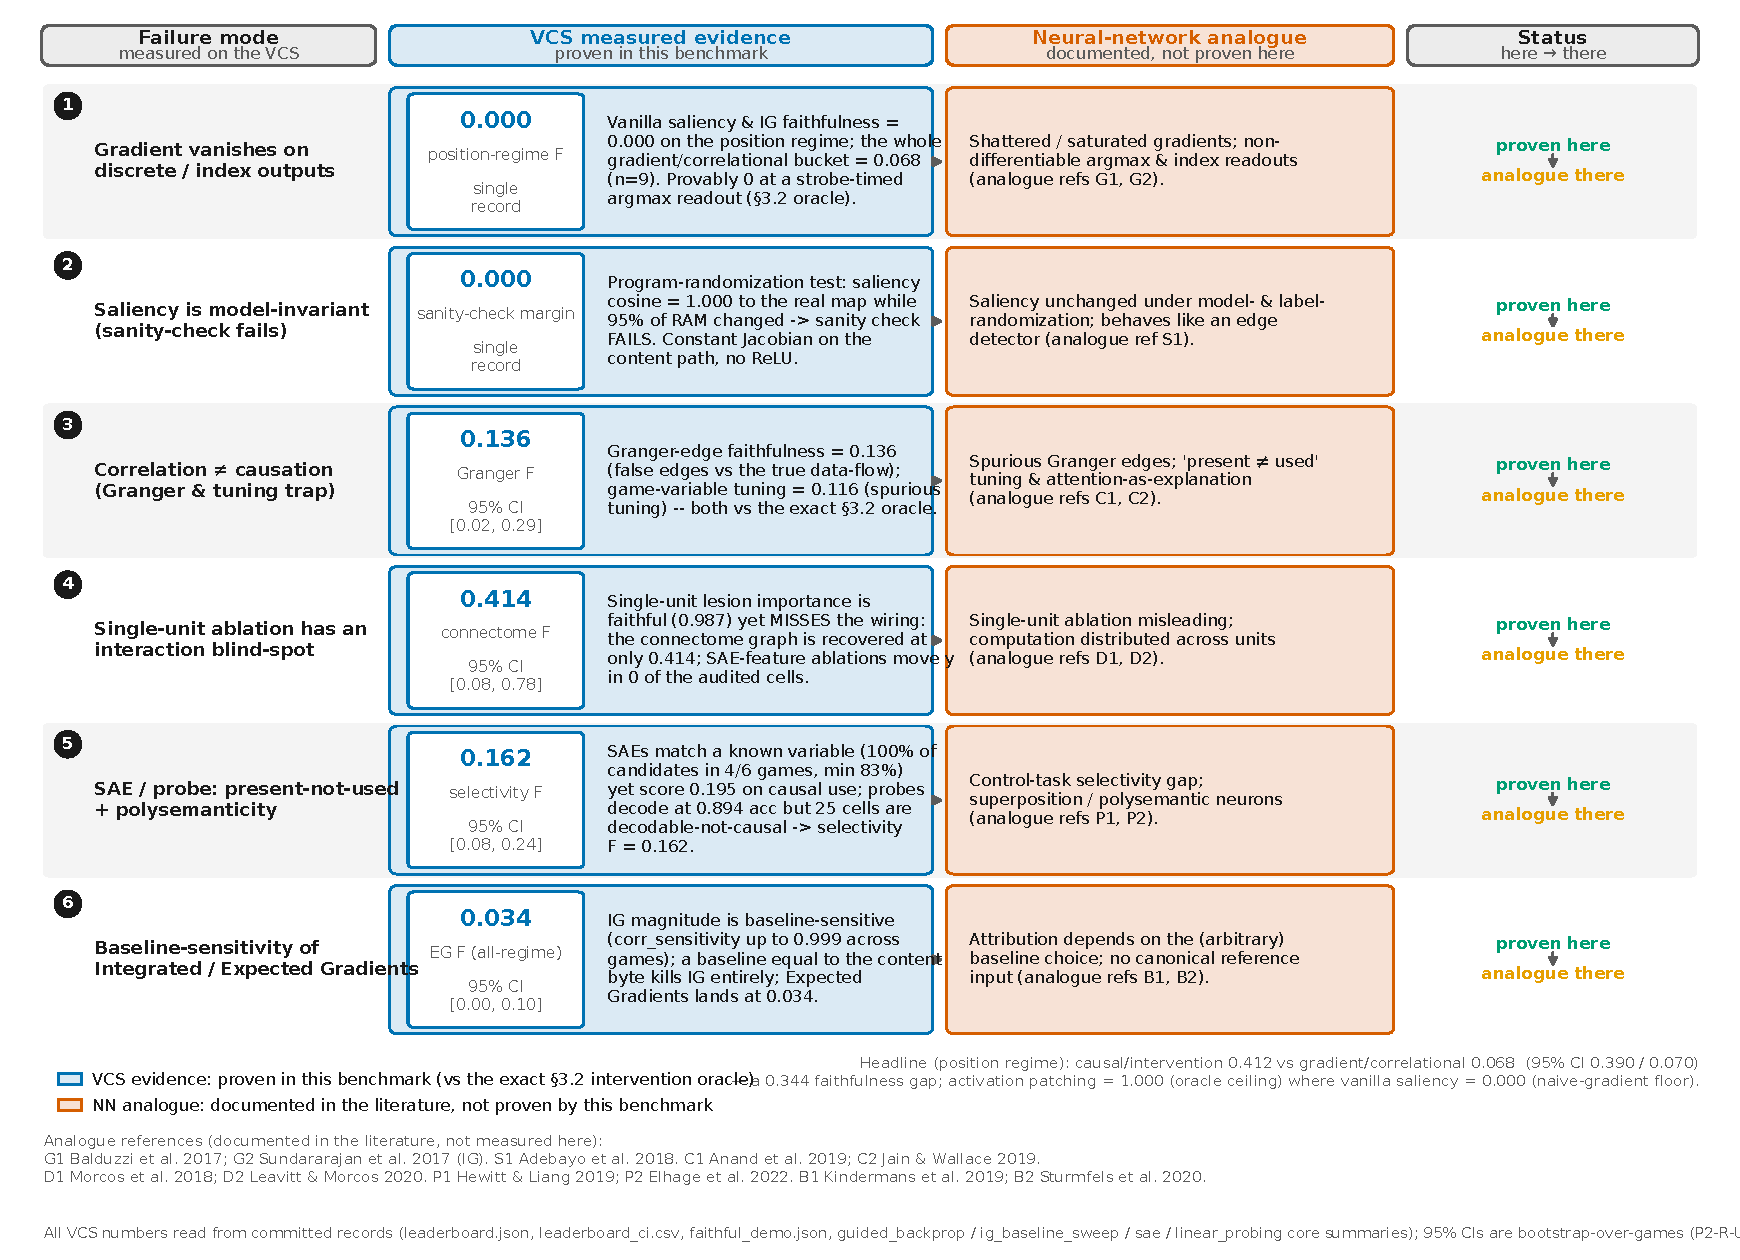
\includegraphics[width=\textwidth]{../figures/fig5_representativeness_map_full.pdf}
\caption{\textbf{Full VCS-to-NN representativeness map.} The full-density version of the
main-text map (Fig.~\ref{fig:representativeness}): each VCS failure mode is placed against its documented
neural-network analogue from the literature. The neural-network column records documented
analogues, not parallels proven by this benchmark; the oracle is the intervention oracle of
\Sectionname3.2, and the underlying per-method values trace to
\texttt{compare/out/leaderboard.json} via Sec.~\ref{supp:provenance}. Note that this full
map is the figure the simplified main-text version condenses.}
\label{supp:fig:repmap}
\end{figure}

\begin{figure}[t]
\centering
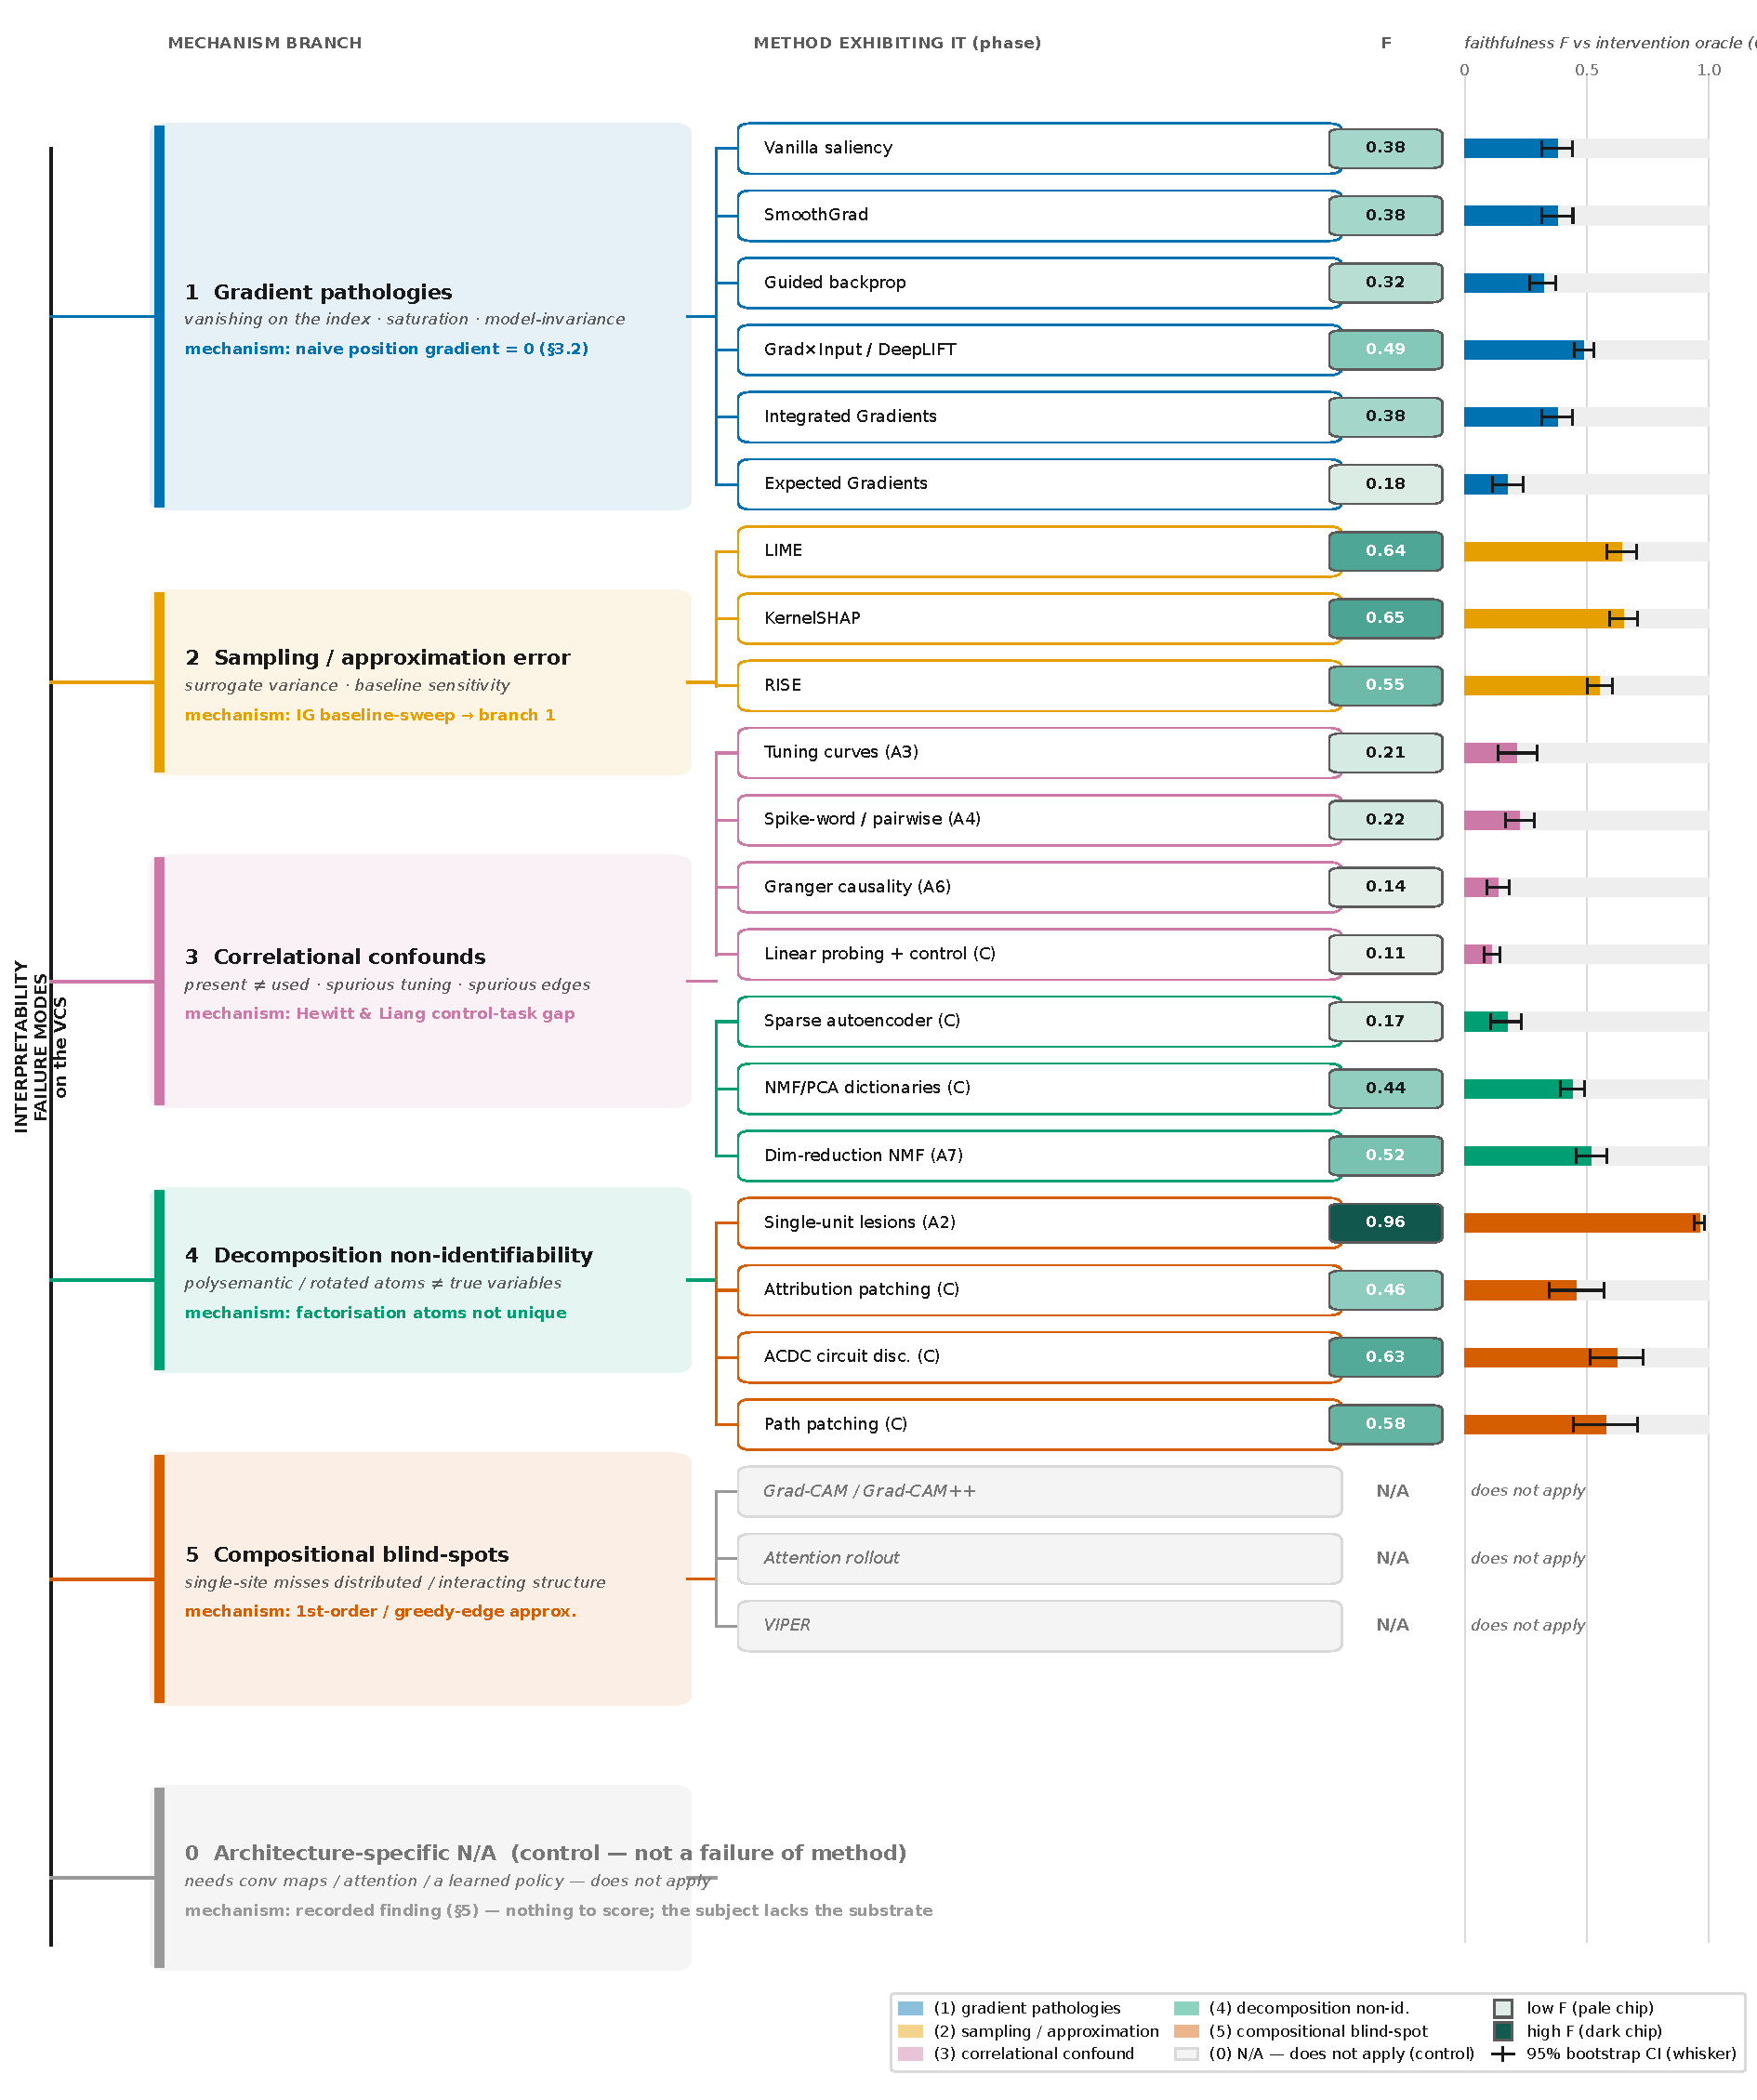
\includegraphics[width=\textwidth]{../figures/fig6_failure_taxonomy_full.pdf}
\caption{\textbf{Full failure taxonomy.} The full-density version of the main-text taxonomy
(Fig.~\ref{fig:taxonomy}): the families of interpretability failure observed on the machine, each annotated
with its faithfulness against the intervention oracle (\Sectionname3.2), reported as $F$ with its
$95\%$ bootstrap confidence interval. The leaf values trace to
\texttt{compare/out/leaderboard.json} and \texttt{leaderboard\_ci.csv} via
Sec.~\ref{supp:provenance}. Note that the gradient and correlational branches collapse on
the discrete position regime, where the naive gradient is provably zero (Prop.~\ref{prop:zero}).}
\label{supp:fig:taxonomy}
\end{figure}

\section{Plausibility-proxy rubric and its sensitivity}\label{supp:plausibility}

The plausibility axis of the leaderboard is a documented, tradition-level proxy, not a
human-subjects measurement. This section records how each value was assigned. It also shows
that the headline contrast does not depend on the particular numbers chosen. The Methods
(\Sectionname\ref{sec:triad}) name two reporting axes. Faithfulness is measured on the machine against the
intervention oracle of \Sectionname\ref{sec:oracle}. The plausibility proxy stands in for how convincing a
tradition's explanations are usually taken to be. We assign the proxy once per method
tradition, before any faithfulness score on our machine is computed, so it cannot be tuned to
the result. Its only job is to expose the danger zone of explanations that look convincing yet
are unfaithful. For that job it must be coarse, fixed in advance, and sourced rather than
precise.

The rubric assigns one proxy per tradition on a fixed five-step scale. It scores two
documented properties of each tradition's typical output and takes their average. The first
property is whether the explanation produces a dense, picture-like artifact that a reader sees
as an account of the computation. Heatmaps and saliency-style maps over the input are read as
convincing by construction. This is the perceptual-immediacy axis. The second property is
whether the field has historically treated the tradition's output as a self-evident
explanation rather than a hypothesis to be tested. This is the adoption-as-explanation axis. A
tradition that scores high on both, such as gradient saliency, receives a high proxy. A
tradition whose output is an austere intervention table or a circuit edge list, rarely
mistaken for a finished story, receives a low one. The scale is deliberately blunt,
$\{0.3,0.5,0.55,0.75,0.8,0.85,0.9\}$. A proxy meant to expose a danger zone gains nothing from
false precision, and a finer scale would invite over-reading. Every value in
Table~\ref{supp:tab:plausrubric} traces to the \jkey{plausibility_proxy} field of the
per-method rows in \texttt{compare/out/leaderboard.json}. The table only groups those rows by
tradition and records the rationale.

\begin{table}[t]
\centering
\caption{\textbf{Plausibility-proxy rubric.} The proxy assigned to each method tradition,
with the documented rationale. Values are the \jkey{plausibility_proxy} field of the
leaderboard rows (\texttt{compare/out/leaderboard.json}). They are tradition-level and fixed
before any faithfulness score is computed, so the proxy cannot be tuned to the measured
faithfulness. A higher value means an explanation that the field tends to find more
convincing, not one that is more faithful. The oracle (\Sectionname\ref{sec:oracle}) is the positive control and
is not a method under test.}
\label{supp:tab:plausrubric}
\begin{tabular}{@{}llp{6.4cm}@{}}
\toprule
Tradition & Proxy & Rationale (documented basis) \\
\midrule
gradient        & $0.90$ & Dense input-space heatmaps read as a visual account of the
                            decision; the most widely adopted XAI outputs, routinely shown
                            as if self-explanatory. \\
probing         & $0.85$ & A trained decoder that ``finds'' a concept reads as evidence the
                            concept is used; high adoption, though decodability is not
                            causal use. \\
correlational   & $0.80$ & Tuning curves and coupling spectra match the neuroscience idiom
                            of a convincing single-unit account. \\
dim.\ reduction & $0.75$ & Low-dimensional factors and dictionary atoms look like a clean
                            summary of the representation. \\
intervention    & $0.55$ & Occlusion and counterfactual outputs are quantitative tables, less
                            immediately picture-like, treated as tests rather than stories. \\
causal          & $0.50$ & Circuit edge lists and patching results are austere artifacts
                            rarely mistaken for a finished narrative. \\
descriptive     & $0.30$ & Whole-state recording is an explicit non-explanation: it withholds
                            nothing and reads as a dump, not an account. \\
\midrule
oracle (control)& $1.00$ & The \Sectionname\ref{sec:oracle} ground truth by construction; positive control, not a
                            method under test. \\
\bottomrule
\end{tabular}
\end{table}

The paper draws a contrast between this proxy and measured faithfulness. On the committed
records the two move in opposite directions. Across the thirty methods under test the Spearman
rank correlation between faithfulness and the proxy is $-0.36$, a negative association.
The traditions the field finds most convincing are, on this machine, among the least faithful.
Eight methods fall in the danger zone, defined here as a proxy of at least $0.70$ together
with a faithfulness below $0.40$. They include the correlational neuroscience methods, Expected
Gradients, guided backprop, linear probing, and the sparse autoencoder. The per-method extreme
makes the point sharply. Vanilla saliency has the highest proxy, $0.9$, yet scores faithfulness
$0.115$ on the position regime. Activation patching has a lower proxy, $0.5$, and scores $1.0$.
Here the less faithful method is the more plausible one. These figures are produced by
\texttt{tools/xai\_study/compare/plausibility\_sensitivity.py} from the leaderboard and
recorded in \texttt{compare/out/plausibility\_sensitivity.csv}.

A proxy fixed by a coarse rubric raises the question of whether the contrast is an artifact of
the particular numbers. The answer is that it is not. We perturb the proxy under four
deterministic schemes and recompute the relationship each time. The analysis uses fixed,
index-keyed offsets rather than random draws, so it re-derives bit-for-bit. The first scheme
adds a fixed per-method jitter of magnitude $\sigma\in\{0.05,0.1,0.2\}$, alternating in sign by
row. The second compresses every proxy toward the common mean by a fraction $\sigma$, which
preserves the rank order of traditions. The third uses the same index-keyed offsets at
$\sigma\in\{0.1,0.2\}$, large enough to swap neighbouring traditions' ranks. The fourth drops
one whole tradition at a time and recomputes on the remainder. Across all fourteen
perturbations the rank correlation between faithfulness and proxy stays negative. It ranges
from $-0.76$ to $-0.08$. The danger zone stays populated, with
between four and ten methods. The per-method anchor sign holds in every scheme where both
anchor methods are present, the more plausible saliency remaining the less faithful. Two runs
bound the range. The strongest is the leave-the-gradient-tradition-out run. It removes the most
plausible and least faithful block at once, and still leaves six danger-zone methods and a rank
correlation of $-0.76$. The weakest is the leave-the-causal-tradition-out run, where the
correlation falls to $-0.08$, close to zero; removing the faithful causal block flattens the
association, so the contrast is carried in part by that block. Table~\ref{supp:tab:plaussens}
reports the full sweep. The contrast keeps its sign under every alternative proxy assignment we
tried: plausibility and faithfulness are not the same axis, and high plausibility is no
guarantee of faithfulness.

\begin{table}[t]
\centering
\caption{\textbf{Proxy-sensitivity sweep.} The faithfulness-versus-proxy relationship under
each perturbation, from \texttt{compare/out/plausibility\_sensitivity.csv}. ``$\rho$'' is the
Spearman rank correlation between faithfulness and proxy over the methods present. ``danger''
is the count of high-proxy ($\geq0.70$), low-faithfulness ($<0.40$) methods. ``anchor'' is
$1$ when the more plausible saliency is the less faithful of the saliency/activation-patching
pair, and blank where a leave-one-out run removes an anchor. The baseline rubric is the first
row. Across every scheme the correlation stays negative and the danger zone stays populated.}
\label{supp:tab:plaussens}
\begin{tabular}{@{}llrrrc@{}}
\toprule
Scheme & Param & $n$ & $\rho$ & Danger & Anchor \\
\midrule
baseline                & ---           & 30 & $-0.36$ &  8 & 1 \\
additive jitter         & $\sigma=0.05$ & 30 & $-0.40$ &  8 & 1 \\
additive jitter         & $\sigma=0.10$ & 30 & $-0.41$ &  8 & 1 \\
additive jitter         & $\sigma=0.20$ & 30 & $-0.42$ & 10 & 1 \\
rank-preserving         & $\sigma=0.10$ & 30 & $-0.36$ &  8 & 1 \\
rank-preserving         & $\sigma=0.20$ & 30 & $-0.36$ &  8 & 1 \\
rank-jittering          & $\sigma=0.10$ & 30 & $-0.41$ &  8 & 1 \\
rank-jittering          & $\sigma=0.20$ & 30 & $-0.42$ & 10 & 1 \\
leave-out causal        & ---           & 24 & $-0.08$ &  8 & \\
leave-out correlational & ---           & 26 & $-0.40$ &  4 & 1 \\
leave-out descriptive   & ---           & 29 & $-0.29$ &  8 & 1 \\
leave-out dim.\ red.    & ---           & 27 & $-0.34$ &  7 & 1 \\
leave-out gradient      & ---           & 20 & $-0.76$ &  6 & \\
leave-out intervention  & ---           & 25 & $-0.34$ &  8 & 1 \\
leave-out probing       & ---           & 29 & $-0.36$ &  7 & 1 \\
\bottomrule
\end{tabular}
\end{table}

; the tables
%% render without overfull boxes and the two SI figures resolve from ../figures/.

\clearpage
\appendix

%% Breakable monospaced JSON key: lets long under_scored keys wrap inside narrow table
%% columns. Used by S5 (number provenance). Defined here so the S-files stay self-contained.
\providecommand{\jkey}[1]{\texttt{\expandafter\jkeyaux#1\relax}}
\makeatletter
\def\jkeyaux#1{\ifx\relax#1\else
  \ifx_#1\discretionary{}{}{}\char`\_\else
    \ifx.#1\discretionary{}{}{}.\else#1\fi\fi
  \expandafter\jkeyaux\fi}
\makeatother

\section*{Supplementary Information}
\setcounter{table}{0}
\setcounter{figure}{0}
\renewcommand{\thetable}{S\arabic{table}}
\renewcommand{\thefigure}{S\arabic{figure}}
\renewcommand{\thesection}{S\arabic{section}}
\setcounter{section}{0}

This Supplementary Information records what the main paper summarizes. We give the
per-method protocols (\Sectionname\ref{supp:protocols}) and the leaderboard schema with its glossary
(\Sectionname\ref{supp:schema}). We give the coverage and applicability of every method across games
and output regimes (\Sectionname\ref{supp:coverage}). We map each headline claim to its evidence
(\Sectionname\ref{supp:claims}). We trace the provenance of every headline number down to the record
file and command that produced it (\Sectionname\ref{supp:provenance}). We state plainly what the
paper does not claim (\Sectionname\ref{supp:notclaimed}). We give the plausibility-proxy rubric and
its sensitivity analysis (\Sectionname\ref{supp:plausibility}). The main text shows simplified forms
of two diagnostic figures; we reproduce both here at full resolution
(Figs.~\ref{supp:fig:repmap} and~\ref{supp:fig:taxonomy}).
The correctness triad $\mathrm{F}\wedge\mathrm{S}\wedge\mathrm{M}$ used throughout is the
one defined in the main Methods (\Sectionname\ref{sec:triad}); we reference it here rather than restating it. The
benchmark scores 30 interpretability methods together with the intervention oracle (\Sectionname\ref{sec:oracle})
as a positive control, for 31 leaderboard rows in total.

\section{Per-method protocols}\label{supp:protocols}

This section records five things for each method under test. It records the exact objects the
method consumes and produces, the reference it is scored against, its sampling or optimization
budget, the metric that turns its output into a faithfulness score, and the committed record
file (version-controlled, in the released repository) that holds the per-game results. All methods share one evaluation contract. We state that
contract once and then specialize it per method. Every method receives the same bit-exact VCS
state on each game of the scored set. We state the contract on the six core games
(\texttt{breakout}, \texttt{ms\_pacman}, \texttt{pong}, \texttt{qbert}, \texttt{seaquest},
\texttt{space\_invaders}), which carry the full tiered ground truth and the exact oracle and
serve as the running example; the aggregate leaderboard scores extend the identical protocol
to the 42-game scored set of \Sectionname\ref{supp:scoredset}. That state is not the boot screen.
It is a shared gameplay state, produced by a single seeded random-action stream (seed~$0$) run
for a $90$-frame prefix and then rolled forward for a $15$-frame analysis horizon. The stream is
deterministic, so every method sees the identical state on each game, and the run is asserted
bit-exact per game. An oracle cause-density gate screens the state before any method runs. The
gate counts how many candidate causes move the output above a floor and rejects states with too
few, so a near-flat oracle column cannot pass. This gate is what turns a degenerate frame into a
usable one; on \texttt{seaquest} it raises the count of live candidate causes from $2$ to $19$.
The candidate-cause set is the machine's own state. This set is the RAM bytes together with the
CPU registers and the TIA and RIOT registers exposed by the substrate. The output every method
attributes over is a shared screen-buffer region read at the end of the analysis horizon, not a
single hand-picked pixel. The reference is the intervention oracle of \Sectionname\ref{sec:oracle},
evaluated by exact re-runs of the emulator under $\mathrm{do}(u)$. A method that
cannot be applied to a given output regime is recorded as not-applicable rather than scored
as zero. An empty result is therefore never read as a wrong one. Faithfulness is the F
axis of the main-text triad (\Sectionname\ref{sec:triad}); we reference that definition and do not restate it.
Records live under \texttt{tools/xai\_study/<phase>/out/}; the aggregate they feed is
\texttt{tools/xai\_study/compare/out/leaderboard.json}.
Table~\ref{supp:leaderboard} consolidates the triad scores for all thirty methods and the
oracle positive control in one place; the per-method protocols follow.

\begin{table*}[t]
\centering
\caption{\textbf{Consolidated leaderboard: all methods, all triad axes.} One row per method
across the three phases, plus the intervention oracle as a positive control. $F$ is
faithfulness (Pearson correlation against the oracle, with the bootstrap-over-games 95\% CI in
brackets), $S$ is sufficiency, $M$ is minimality, all as defined in \Sectionname\ref{sec:triad};
Plaus is the elicited plausibility prior and $n$ is the number of scored games. Attribution
methods that emit only a saliency have no defined $S$ or $M$ and are marked ``---''; A5
(field potentials) and A7 (dimensionality reduction) likewise lack the $S$/$M$ decomposition.
Values are transcribed from \texttt{tools/xai\_study/compare/out/leaderboard.json} (the
committed numbers of record).}
\label{supp:leaderboard}
\footnotesize
\setlength{\tabcolsep}{4pt}
\begin{tabularx}{\textwidth}{@{}Xccccccc@{}}
\toprule
Method & Phase & Tradition & $F$ (95\% CI) & $S$ & $M$ & Plaus & $n$ \\
\midrule
A1 connectomics & A & intervention & 0.207 [0.130, 0.293] & 0.971 & 0.967 & 0.55 & 35 \\
A2 lesions & A & intervention & 0.965 [0.942, 0.983] & 0.591 & 1.000 & 0.55 & 42 \\
A3 tuning curves & A & correlational & 0.213 [0.136, 0.295] & 0.200 & 0.928 & 0.80 & 42 \\
A4 spike-word / pairwise & A & correlational & 0.225 [0.166, 0.283] & 0.133 & 0.363 & 0.80 & 34 \\
A5 field potentials & A & correlational & 0.376 [0.323, 0.428] & --- & --- & 0.80 & 40 \\
A6 Granger & A & correlational & 0.136 [0.091, 0.184] & 0.884 & 0.647 & 0.80 & 35 \\
A7 dim.\ reduction & A & dim.\ red. & 0.519 [0.457, 0.581] & --- & --- & 0.75 & 42 \\
A8 whole-state & A & descriptive & 1.000 [1.000, 1.000] & 1.000 & 0.075 & 0.30 & 42 \\
\midrule
Vanilla saliency & B & gradient & 0.380 [0.316, 0.445] & --- & --- & 0.90 & 42 \\
smoothgrad & B & gradient & 0.380 [0.317, 0.445] & --- & --- & 0.90 & 42 \\
Guided backprop & B & gradient & 0.322 [0.267, 0.375] & --- & --- & 0.90 & 42 \\
Grad$\times$Input / DeepLIFT & B & gradient & 0.486 [0.448, 0.526] & --- & --- & 0.90 & 42 \\
Integrated Gradients & B & gradient & 0.379 [0.314, 0.444] & --- & --- & 0.90 & 42 \\
Expected Gradients & B & gradient & 0.175 [0.110, 0.240] & --- & --- & 0.90 & 42 \\
kernelshap & B & gradient & 0.652 [0.596, 0.709] & --- & --- & 0.90 & 42 \\
lime & B & gradient & 0.644 [0.582, 0.705] & --- & --- & 0.90 & 42 \\
rise & B & gradient & 0.552 [0.500, 0.600] & --- & --- & 0.90 & 42 \\
occlusion & B & intervention & 0.687 [0.624, 0.746] & --- & --- & 0.55 & 42 \\
Extremal perturbation & B & intervention & 0.461 [0.410, 0.513] & --- & --- & 0.55 & 42 \\
On-distribution counterfactual & B & intervention & 0.433 [0.343, 0.522] & --- & --- & 0.55 & 42 \\
\midrule
Activation patching & C & causal & 1.000 [1.000, 1.000] & --- & --- & 0.50 & 42 \\
Causal scrubbing & C & causal & 0.979 [0.940, 1.000] & 0.979 & 0.814 & 0.50 & 42 \\
Interchange interventions (DAS) & C & causal & 1.000 [1.000, 1.000] & --- & --- & 0.50 & 42 \\
Logit / tuned lens & C & causal & 0.820 [0.768, 0.871] & --- & 0.224 & 0.50 & 42 \\
Path patching & C & causal & 0.580 [0.452, 0.710] & --- & --- & 0.50 & 42 \\
ACDC & C & causal & 0.625 [0.514, 0.730] & 0.299 & 1.000 & 0.50 & 35 \\
Attribution patching & C & gradient & 0.456 [0.345, 0.573] & --- & --- & 0.90 & 42 \\
Linear probing (+ control) & C & probing & 0.240 [0.153, 0.346] & --- & 0.932 & 0.85 & 42 \\
NMF / PCA dictionaries & C & dim.\ red. & 0.102 [0.049, 0.160] & 0.751 & 0.966 & 0.75 & 42 \\
Sparse autoencoder & C & dim.\ red. & 0.153 [0.096, 0.218] & 0.183 & 0.934 & 0.75 & 40 \\
\midrule
Intervention oracle & --- & oracle & 1.000 [1.000, 1.000] & 1.000 & 1.000 & 1.00 & 1 \\
\bottomrule
\end{tabularx}
\end{table*}

The neuroscience analyses (Phase~A) treat the running machine as a brain. It asks how far
each classical analysis recovers the known mechanism on the shared gameplay state. Each
method's baseline is the exact data-flow graph or causal role that the substrate makes
available. Its budget is the scored set (\Sectionname\ref{supp:scoredset}) unless noted,
with the six-game core as the running example, and its scoring metric is named in
Table~\ref{supp:tab:phaseA}. One core cell is honestly degenerate. On \texttt{ms\_pacman} the
pairwise analysis (A4) finds no coupled candidate pair to score at that frame, so its
\texttt{ms\_pacman} value is uninformative rather than a failure; the other five games carry
it.

\begin{table}[t]
\centering
\caption{\textbf{Phase~A protocols (neuroscience analyses).} One row per method. The columns
give the input it reads, the reference it is scored against, the sampling or intervention
budget, the scoring metric, and the committed record. All eight run on the scored set
(\Sectionname\ref{supp:scoredset}), with the six core games as the running example;
faithfulness is the F axis of \Sectionname\ref{sec:triad}. The whole-state recording (A8) is included as a
descriptive upper bound on coverage. Its faithfulness $F$ is trivial, so we read it for its
minimality $M$.}
\label{supp:tab:phaseA}
\scriptsize
\setlength{\tabcolsep}{4pt}
\begin{tabular}{@{}p{1.7cm}p{2.6cm}p{1.9cm}p{2.6cm}p{1.0cm}@{}}
\toprule
Method & Input / candidate causes & Reference & Scoring metric & Record \\
\midrule
A1 connectomics & RAM/register activity over trajectory & data-flow graph & data-flow graph $F_1$ vs.\ oracle & A1 \\
A2 lesions & single-cell knockouts via $\mathrm{do}(u)$ & true causal role & lesion-importance $\rho$ vs.\ role & A2 \\
A3 tuning curves & per-cell response vs.\ variable & variable coupling & $1-$ spurious-tuning rate & A3 \\
A4 spike-word / pairwise & pairwise cell correlations & true coupling & corr.\ $\rho$ vs.\ coupling & A4 \\
A5 field potentials & pooled-activity spectra & true causal share & $1-$ clock-explained var. & A5 \\
A6 Granger & directed lag structure & true data-flow & $1-$ false-edge rate & A6 \\
A7 dim.\ reduction & NMF/PCA over activity & known variables & NMF matched-component frac. & A7 \\
A8 whole-state & full state record & oracle decomp. & minimality $M$ vs.\ oracle & A8 \\
\bottomrule
\end{tabular}

\smallskip
\noindent\scriptsize Records: \texttt{tools/xai\_study/phaseA\_kording/out/A\{1..8\}\_*}; all
eight run on the 42-game scored set (\Sectionname\ref{supp:scoredset}), with the six core
games as the running example (\jkey{n_games} per method in \jkey{leaderboard.json}).
\end{table}

The attribution methods (Phase~B) run the everyday XAI toolbox over the same gameplay state.
These methods produce a real-valued saliency or attribution over the candidate-cause set.
We score that output by Pearson correlation against the oracle attribution. The gradient family
runs with the bilinear sub-pixel sampler turned on, so it is scored on a real position gradient
and not on the naive one. The naive gradient of the discrete position output is provably zero
(Prop.~\ref{prop:zero}); the sampler restores a finite gradient, but the restored gradient is
low and mixed in faithfulness rather than a fix. Expected Gradients draws its reference pool
from the states of the same seeded gameplay trajectory, not from a synthetic baseline. Two cells
are honestly degenerate and recorded as such. The on-distribution counterfactual returns a zero
delta on \texttt{space\_invaders}, \texttt{ms\_pacman}, and \texttt{qbert}, where its perturbation
does not move the shared output at that frame; those cells are marked not-valid rather than
scored. Expected Gradients scores low on the content regime of every game except \texttt{pong},
because the causal byte it should land on is static there. The budgets that matter are the
Monte-Carlo or perturbation counts of the sampling estimators, recorded per method in
Table~\ref{supp:tab:phaseB}. The seed-dispersion of the stochastic members is carried in
\texttt{leaderboard\_ci.csv} (\texttt{seed\_sd}, \texttt{seed\_sd\_source}) and reproduced
in \Sectionname\ref{supp:provenance}.

\begin{table}[t]
\centering
\caption{\textbf{Phase~B protocols (attribution methods).} Each method emits a saliency over
the candidate-cause set. We score it by Pearson correlation against the oracle attribution
(\Sectionname\ref{sec:oracle}). The reference is shared and the budget is the scored set of
\Sectionname\ref{supp:scoredset} (six core games as the running example). The budget column records the
sampling or perturbation count that drives each estimator. The seed column flags which
methods carry an independent-seed dispersion in \texttt{leaderboard\_ci.csv}.}
\label{supp:tab:phaseB}
\scriptsize
\setlength{\tabcolsep}{4pt}
\begin{tabular}{@{}p{2.9cm}p{1.75cm}p{4.3cm}p{1.15cm}@{}}
\toprule
Method & Tradition & Budget / hyperparameters & Seed sd \\
\midrule
Vanilla saliency & gradient & single backward pass & --- \\
smoothgrad & gradient & noise-averaged gradient; $\sigma$-robustness committed & 0.0 \\
Guided backprop & gradient & single guided pass & --- \\
Grad$\times$Input / DeepLIFT & gradient & DeepLIFT reference-difference & --- \\
Integrated Gradients & gradient & path integral, baseline = zero state & --- \\
Expected Gradients & gradient & expectation over baselines (refits) & yes \\
kernelshap & gradient & Monte-Carlo coalition sampling ($\propto 1/\sqrt{N}$) & 0.017 \\
lime & gradient & local linear fit, perturbation refits & 0.029 \\
rise & gradient & random-mask Monte-Carlo ($\propto 1/\sqrt{N}$) & 0.051 \\
occlusion & intervention & exhaustive single-cell masking & --- \\
Extremal perturbation & intervention & optimized mask, area-constrained & --- \\
On-distribution counterfactual & intervention & on-manifold $\mathrm{do}(u)$ resampling & --- \\
\bottomrule
\end{tabular}

\smallskip
\noindent\scriptsize Records: \texttt{tools/xai\_study/phaseB\_attribution/out/}; all twelve run
on the 42-game scored set (\Sectionname\ref{supp:scoredset}), six core games as the running
example, and are scored by Pearson correlation against the oracle (\Sectionname\ref{sec:oracle}). Seed
sd is the independent-seed dispersion from \texttt{leaderboard\_ci.csv}.
\end{table}

The mechanistic methods (Phase~C) are built to recover circuits. Each is scored
against the true data-flow or the exact recovered-minus-exact deviation. The causal members
of this phase are the ones that reach the oracle ceiling. We list their exact scoring metric
so that the ceiling is not read as a tautology. Each member is scored against the substrate's
known routine, and not against another method. Two members (NMF/PCA dictionaries and the
sparse autoencoder) are dimensionality-reduction methods carried here for comparison. The
sparse autoencoder has two aggregations that differ, which we reconcile in
\Sectionname\ref{supp:provenance}.

\begin{table}[t]
\centering
\caption{\textbf{Phase~C protocols (mechanistic methods).} Each method is scored against the
substrate's known circuit or the exact recovered-minus-exact deviation (\Sectionname\ref{sec:oracle}), and not
against another method. This is what keeps the oracle ceiling non-circular. The probing and
dictionary-learning members are included for comparison with the causal members.}
\label{supp:tab:phaseC}
\scriptsize
\setlength{\tabcolsep}{4pt}
\begin{tabular}{@{}p{3.4cm}p{1.4cm}p{5.2cm}@{}}
\toprule
Method & Tradition & Scoring metric \\
\midrule
Activation patching & causal & $\max|\text{recovered}-\text{exact}|$ vs.\ oracle \\
Causal scrubbing & causal & scrubbing-preserved performance \\
Interchange interventions (DAS) & causal & aligned interchange accuracy \\
Logit / tuned lens & causal & logit-lens fidelity to true intermediate \\
Path patching & causal & path-circuit $F_1$ vs.\ true routine \\
ACDC & causal & discovered-circuit best $F_1$ vs.\ data-flow \\
Attribution patching & gradient & corr.\ of approximation vs.\ exact patch \\
Linear probing (+ control) & probing & selectivity vs.\ control task \\
NMF / PCA dictionaries & dim.\ red. & matched-component fraction vs.\ vars \\
Sparse autoencoder & dim.\ red. & feature-variable matched fraction \\
\bottomrule
\end{tabular}

\smallskip
\noindent\scriptsize Records: \texttt{tools/xai\_study/phaseC\_mechanistic/out/}; all ten run
on the 42-game scored set (\Sectionname\ref{supp:scoredset}), with the six core games as the
running example.
\end{table}

The intervention oracle is the positive control, not a method under test. It is the exact
$\mathrm{do}(u)$ ground truth of \Sectionname\ref{sec:oracle}, evaluated by re-running the bit-exact machine. It
attains $F=S=M=1.0$ by construction. Its record triple is the intervention oracle, the
content-path gradient oracle, and their cross-check
(\texttt{tools/xai\_study/ground\_truth/out/}). It anchors the ceiling against which every
other row is read, which is why it occupies the thirty-first leaderboard row.

\section{Benchmark schema and glossary}\label{supp:schema}

The leaderboard is built from a flat record schema. Stating it removes the ambiguity
about what a single number on the benchmark counts. Each method is run per game and writes a
per-game record under its phase's \texttt{out/} tree. The leaderboard aggregates those
records into one row per method by averaging over games. The schema columns of a leaderboard
row are given in Table~\ref{supp:tab:schema}. The aggregation rule is a mean over the
$n_{\text{games}}$ games. When a method emits several output records on one game, those records
are first reduced within that game. The faithfulness, sufficiency, and minimality columns
report the F, S, and M axes defined in \Sectionname\ref{sec:triad}. We do not re-derive those definitions here.

\begin{table}[t]
\centering
\caption{\textbf{Leaderboard row schema.} The columns of one row in
\texttt{compare/out/leaderboard.json} (\texttt{rows[\,]}) and its uncertainty companion
\texttt{leaderboard\_ci.csv}. The metric column names the per-method scoring function from
\Sectionname\ref{supp:protocols}; F, S, and M are the triad axes of \Sectionname\ref{sec:triad}. Aggregation is a mean
over $n_{\text{games}}$, with bootstrap confidence intervals over games (and, where present,
over records).}
\label{supp:tab:schema}
\footnotesize
\begin{tabular}{@{}p{3.0cm}p{8.4cm}@{}}
\toprule
Column & Meaning \\
\midrule
\texttt{phase} & phaseA\_kording, phaseB\_attribution, phaseC\_mechanistic, or ground\_truth \\
\texttt{method} & method identifier (the row key) \\
\texttt{tradition} & intervention, causal, gradient, correlational, \jkey{dim_reduction}, probing, descriptive, oracle \\
\jkey{n_games} & number of games the method was scored on (up to 42 for the scored set of \Sectionname\ref{supp:scoredset}; 1 for the oracle) \\
\jkey{n_records} & number of per-game output records aggregated into the row \\
\texttt{faithfulness} (F) & faithfulness vs.\ the intervention oracle (\Sectionname\ref{sec:oracle}), $[0,1]$, higher better \\
\jkey{faithfulness_ci95} & $95\%$ bootstrap CI half-width over games \\
\jkey{faithfulness_position_regime} & F restricted to the discrete sprite-position/index regime \\
\jkey{faithfulness_content_regime} & F restricted to the continuous content regime \\
\texttt{triad\_S} / \texttt{triad\_M} & sufficiency / minimality axes (\Sectionname\ref{sec:triad}), where applicable \\
\jkey{plausibility_proxy} & documented method-tradition proxy, $[0,1]$ --- not a human-subjects measurement \\
\jkey{is_positive_control} & 1 for the oracle row, 0 otherwise \\
\jkey{metric_names} & the per-method scoring function (\Sectionname\ref{supp:protocols}) \\
\texttt{commits} & the commit(s) at which the per-game records were produced \\
\bottomrule
\end{tabular}
\end{table}

We fix the vocabulary that the schema implies, because the review asked for a single
unambiguous method count. A \emph{method} is one interpretability technique, e.g.\
\texttt{vanilla\_saliency}. A \emph{method row} is its single aggregated line on the
leaderboard. A \emph{per-game record} is one method scored on one game, written under a phase
\texttt{out/} tree. An \emph{output record} is a per-game record for one output regime; a
method may emit several of these on one game. A \emph{family mean} is the average over the
members of a tradition family, e.g.\ causal/intervention. The \emph{oracle positive control}
is the exact $\mathrm{do}(u)$ ground truth of \Sectionname\ref{sec:oracle}, scored as a method to anchor the
ceiling. A \emph{not-applicable method} is one that does not apply to a given output regime;
it is recorded as N/A rather than as a zero. With this vocabulary the count is unambiguous.
The benchmark scores 30 interpretability methods together with the intervention
oracle as a positive control, for 31 leaderboard rows in total
(\texttt{leaderboard.json.n\_methods}~$=31$), aggregating 1773 per-game records over the
42-game scored set (\texttt{n\_per\_game\_records\_aggregated}~$=1773$): 8 methods in
Phase~A, 12 in Phase~B, 10 in Phase~C, and the one oracle row. This count is the canonical one
used in the abstract, the figures, and throughout this Supplement.

\section{Coverage and applicability}\label{supp:coverage}

The benchmark scores methods on a six-game core drawn from a larger bit-exact substrate. The
coverage table makes the scope of that choice explicit. Paper~1 validates the
differentiable VCS ports bit-for-bit against the \texttt{xitari} reference on all 64 Arcade
Learning Environment games, within a 30-frame RAM and 60-frame screen window. The
interpretability study reported here runs on the six games listed in
Table~\ref{supp:tab:coverage}. Every method is scored on a shared gameplay state, produced by
one seeded random-action stream (seed~$0$, $90$-frame prefix, $15$-frame analysis horizon), not
on the boot screen. This keeps the analysis inside the Paper~1 bit-exact window while giving the
oracle a rich, non-degenerate cause set to score against. We pick these six games because all
three tiers of ground truth (\Sectionname\ref{sec:tiers}) are available for them and the oracle is
exact. The remaining 58 games are
bit-exact substrate but are not scored here. Some fall outside the validated horizon for the
analyses we run. For others, the tiered labels they would need are not yet produced. They are
candidates for the larger sweep, and are not excluded for any methodological reason. The
horizon column records the validated window. The tier column records which of the three
ground-truth tiers (T1 exact intervention, T2 data-flow, T3 externally-supplied semantic
labels) is available.

\begin{table}[t]
\centering
\caption{\textbf{Core-game coverage.} The six core games carry exact tiered ground truth and
the full method battery. Faithfulness is scored within the Paper~1 bit-exact window. The
last two columns give the methods run and the per-game output records contributed. The wider
64-game substrate is bit-exact (Paper~1) but is reserved for the larger sweep. T3 labels are
external (\Sectionname\ref{sec:tiers}); we record this so the benchmark does not appear to certify them.}
\label{supp:tab:coverage}
\footnotesize
\setlength{\tabcolsep}{4pt}
\begin{tabular}{@{}p{2.4cm}p{1.9cm}p{1.5cm}p{1.7cm}p{1.5cm}p{1.4cm}@{}}
\toprule
Game & Paper-1 status & Horizon & Tiers & Methods run & Records \\
\midrule
breakout & bit-exact & 30/60 fr & T1,T2,T3 & 30 + oracle & per-game \\
ms\_pacman & bit-exact & 30/60 fr & T1,T2,T3 & 30 + oracle & per-game \\
pong & bit-exact & 30/60 fr & T1,T2,T3 & 30 + oracle & per-game \\
qbert & bit-exact & 30/60 fr & T1,T2,T3 & 30 + oracle & per-game \\
seaquest & bit-exact & 30/60 fr & T1,T2,T3 & 30 + oracle & per-game \\
space\_invaders & bit-exact & 30/60 fr & T1,T2,T3 & 30 + oracle & per-game \\
\midrule
58 further games & bit-exact (P1) & 30/60 fr & T1,T2 partial & reserved & --- \\
\bottomrule
\end{tabular}
\end{table}

A gameplay state can still be degenerate for a particular method, and the benchmark records
this rather than scoring it as a failure. The oracle cause-density gate is the first guard. It
counts how many candidate causes move the shared output above a floor, and rejects a state that
does not clear a minimum count, so a near-flat oracle column never reaches a method. On
\texttt{seaquest} the gate raises the count of live candidate causes at the analysis frame from
$2$ to $19$, which is what makes the game usable. Three residual degenerate cells survive the
gate and are marked, not scored as zero. On \texttt{ms\_pacman} the pairwise neuroscience
analysis (A4) finds no coupled candidate pair at that frame, so its cell is uninformative. The
on-distribution counterfactual returns a zero delta on \texttt{space\_invaders},
\texttt{ms\_pacman}, and \texttt{qbert}, where its perturbation does not move the shared output;
those cells are recorded as not-valid. Expected Gradients scores low on the content regime of
every game but \texttt{pong}, because the causal byte it should attribute to is static there.
None of these cells is read as a wrong answer.

Whether a method applies at all depends on what the method needs from its target. The
applicability matrix records that for every method family. The Phase~A neuroscience analyses
read the raw machine state and need neither a learned policy nor gradients. The Phase~B
attribution methods split into two groups. The gradient members need a differentiable forward
pass. The intervention members need only the ability to set state. The Phase~C mechanistic
methods need access to internal activations. The causal members among them also need the
ability to intervene. Table~\ref{supp:tab:applic} records, per family, whether the method
operates on the raw VCS, whether it requires a learned policy, gradients, internal layers or
attention, or external labels, whether it uses oracle-like interventions, and whether it
receives a supplied hypothesis. The table shows the same pattern the results confirm. The
families that score high on faithfulness are the ones that can intervene. The families that
collapse on the position regime are the gradient and correlational ones.

\begin{table}[t]
\centering
\caption{\textbf{Per-family applicability.} What each method family requires of its target.
``Intervenes'' marks oracle-like $\mathrm{do}(u)$ access; ``hypothesis'' marks methods that
receive a supplied circuit hypothesis to test. The raw-VCS column distinguishes analyses that
read machine state directly from those that need a differentiable or layered model. A blank
means the requirement does not apply.}
\label{supp:tab:applic}
\footnotesize
\begin{tabular}{@{}p{3.0cm}cccccc@{}}
\toprule
Family & raw VCS & policy & gradients & layers/attn & intervenes & hypothesis \\
\midrule
A neuroscience & yes & no & no & no & A2 only & no \\
B gradient & yes & no & yes & no & no & no \\
B intervention & yes & no & no & no & yes & no \\
C causal & yes & no & no & yes & yes & yes \\
C gradient (attr.\ patch) & yes & no & yes & yes & approx. & yes \\
C probing & yes & no & no & yes & no & no \\
C / A dim.\ reduction & yes & no & no & yes & no & no \\
oracle (control) & yes & no & no & yes & exact & --- \\
\bottomrule
\end{tabular}
\end{table}

\section{Claims and evidence}\label{supp:claims}

Every headline claim in the paper rests on a specific artifact. The table in this section
makes that dependency checkable. For each claim we list the figure or table that supports it,
the games and methods it uses, the metric, the artifact it traces to, and the limitation that
bounds it. Faithfulness, sufficiency, and minimality are the three axes of \Sectionname\ref{sec:triad}.
The numbers themselves are sourced in \Sectionname\ref{supp:provenance}. The table below names which
evidence supports which claim; it does not repeat the values. One split matters for how the
table is read. The all-regime faithfulness gap between causal/intervention and
gradient/correlational methods is $0.297$ with a $95\%$ interval of $[0.232,0.375]$ that
excludes zero, and it is the primary evidence for the headline. The position-only gap is
$0.238$ with an interval of $[-0.049,0.315]$ that crosses zero at six games. We report the
position gap as directional support, not as a significant result.

\begin{table}[t]
\centering
\caption{\textbf{Claims and their evidence.} Each headline claim maps to the figure or table
that supports it, the games and methods involved, the metric, the committed artifact, and the
limitation that bounds the claim. The artifact column points to the record that
\Sectionname\ref{supp:provenance} traces to a value. The limitation column states the scope, so the
claim is not read wider than the evidence.}
\label{supp:tab:claims}
\scriptsize
\setlength{\tabcolsep}{4pt}
\begin{tabular}{@{}p{3.0cm}p{1.9cm}p{1.8cm}p{1.9cm}p{2.4cm}@{}}
\toprule
Claim & Evidence & Methods / games & Metric & Limitation \\
\midrule
Causal/intervention methods beat gradient/correlational on faithfulness across all regimes & Fig.~\ref{fig:faithfulness}; leaderboard & 25 methods, 6 games & F mean (gap $0.297$) & robust: gap $0.297$ $[0.232,0.375]$ excludes zero; this all-regime gap is the primary evidence \\
The gap holds with the same sign on the discrete position regime & Fig.~\ref{fig:faithfulness}; \jkey{faithful_demo} & 13 rows, 6 games & F position (gap $0.238$) & directional only: gap $0.238$ $[-0.049,0.315]$ crosses zero at 6 games, so it is not significant \\
A faithful causal method reaches the oracle ceiling where the default tool stays low & \jkey{faithful_demo}; Fig.~\ref{fig:faithfulness} & act.\ patching vs.\ vanilla saliency, 6 games & F $1.0$ vs.\ $0.165$ (position regime; all-regimes saliency F $0.419$, plotted in Fig.~\ref{fig:faithfulness}) & one decisive pair \\
The naive gradient of a discrete position output is provably zero & Prop.~\ref{prop:zero} (\Sectionname\ref{sec:oracle}); \jkey{oracle_grad} & all gradient methods & grad@position $=0$; sampler restores $166$ & position path only; restored gradient is low/mixed \\
High plausibility coexists with low faithfulness (the danger zone) & Fig.~\ref{fig:faithfulness}; \jkey{faithful_demo} & vanilla saliency & proxy $0.9$, F $0.165$ (position regime; all-regimes F $0.419$, plotted in Fig.~\ref{fig:faithfulness}) & proxy, not measured plausibility \\
Faithful attribution recovers the wiring but not the computation's semantics & Fig.~\ref{fig:taxonomy} (\Sectionname\ref{supp:coverage}); discussion & Phase~B vs.\ C & F vs.\ S, M & necessary-condition stress test \\
The failure modes have documented NN analogues & Fig.~\ref{fig:representativeness} & taxonomy & --- & analogues, not proof \\
\bottomrule
\end{tabular}
\end{table}

\section{Number provenance}\label{supp:provenance}

Every headline number traces to a committed record, the script that produced it, and the
command that re-derives it. This section is the in-paper copy of that traceability table. It
mirrors \Sectionname6.5 of the reproducibility document
(\texttt{xai\_2\_interpretability/REPRODUCIBILITY.md}). The values are the measured, committed
ones at the current revision. The position-regime gap and its $95\%$ interval are read from
\texttt{tools/xai\_study/compare/out/position\_bootstrap.json}; the other aggregates from
\texttt{leaderboard.json}, rather than recomputed here. Each
record also carries \texttt{seed}, \texttt{where}, \texttt{commit}, and \texttt{timestamp}, so
the provenance of every value is self-documenting. The aggregate scores below are taken over
the 42-game scored battery of \Sectionname\ref{supp:scoredbattery}, not the six-game core;
each per-method row is a mean over the games on which that method applies (\jkey{n_games}
per method, e.g.\ 42 for most methods, 35 for ACDC and A1). The position-regime gap is now
significant on this battery.

\begin{table}[t]
\centering
\caption{\textbf{Headline-number provenance.} Each number $\rightarrow$ its committed record
and JSON key $\rightarrow$ the generating or aggregating script $\rightarrow$ the command
that reproduces it. Values are the measured, committed numbers at this revision (consistent
with REPRODUCIBILITY \Sectionname6.5); the position-regime gap CI is read from
\jkey{position_bootstrap.json}, all other aggregates from \jkey{leaderboard.json}. Paths are
relative to \texttt{tools/xai\_study/}.}
\label{supp:tab:provenance}
\scriptsize
\setlength{\tabcolsep}{3pt}
\renewcommand{\arraystretch}{1.15}
\begin{tabular}{@{}p{2.5cm}p{1.6cm}p{3.4cm}p{1.9cm}@{}}
\toprule
Number & Value & Record (JSON key) & Command \\
\midrule
Faithfulness gap, all regimes (causal $-$ gradient) & $0.3374$\newline {\scriptsize$[0.3103,0.3643]$, excl.\ $0$} & \jkey{position_bootstrap.json}: \jkey{all\_regime.family\_mean\_gap}, \jkey{ci95} & \jkey{position_bootstrap.py} \\
Causal/interv.\ mean F, all regimes & $0.7215$\newline {\scriptsize$n{=}11$} & \jkey{leaderboard.json}: \jkey{family_causal_intervention} \jkey{mean} & \jkey{leaderboard.py} \\
Gradient/corr.\ mean F, all regimes & $0.384$\newline {\scriptsize$n{=}14$} & \jkey{leaderboard.json}: \jkey{family_gradient_correlational} \jkey{mean} & \jkey{leaderboard.py} \\
Faithfulness gap, position regime (bootstrap over games) & $0.3268$\newline {\scriptsize$[0.1325,0.3702]$, excl.\ $0$} & \jkey{position_bootstrap.json}: \jkey{family_mean_gap}, \jkey{ci95} & \jkey{position_bootstrap.py} \\
Causal/interv.\ mean F, position regime & $0.561$\newline {\scriptsize$\pm0.3212$, $n{=}4$} & \jkey{leaderboard.json}: \jkey{family_..._intervention_position} \jkey{mean} & \jkey{leaderboard.py} \\
Gradient/corr.\ mean F, position regime & $0.2343$\newline {\scriptsize$\pm0.156$, $n{=}9$} & \jkey{leaderboard.json}: \jkey{family_..._correlational_position} \jkey{mean} & \jkey{leaderboard.py} \\
Decisive pair, position regime (act.\ patch vs.\ vanilla sal.) & $1.000$\newline vs.\ $0.115$ & \texttt{faithful\_demo}: \jkey{pair_contrast} & \jkey{faithful_demo.py} \\
Plausibility proxy, decisive pair & $0.5$ vs.\ $0.9$ & \texttt{faithful\_demo}: \jkey{...plausibility_proxy} & \jkey{faithful_demo.py} \\
ACDC sufficiency $S$ & $0.299$ & \jkey{leaderboard.json}: ACDC \jkey{triad_S} & \jkey{leaderboard.py} \\
Whole-state minimality $M$ & $0.0755$ & \jkey{leaderboard.json}: A8 \jkey{triad_M} & \jkey{leaderboard.py} \\
Methods scored (rows) & $31$ & \texttt{leaderboard}: \jkey{n_methods} & \jkey{leaderboard.py} \\
Per-game records aggregated & $1773$ & \texttt{leaderboard}: \jkey{n_per_game_records_aggregated} & \jkey{leaderboard.py} \\
Naive gradient, discrete position output & position $0$;\newline content $1.0$; sampler $166$ & \jkey{oracle_grad_pong.json}: \texttt{value}, \jkey{extra.sampler} & \jkey{oracle_grad.jl} \\
Exact oracle $\max|\Delta\text{score}|$ (Pong) & $17.0$ & \jkey{oracle_pong_score.json}: \texttt{value} & \jkey{oracle_intervene.jl} \\
\bottomrule
\end{tabular}

\smallskip
\noindent\scriptsize Scripts live under \texttt{tools/xai\_study/compare/} (Python) and
\texttt{tools/xai\_study/ground\_truth/} (Julia); records under the corresponding \texttt{out/}
trees. JSON keys are abbreviated with ``\texttt{...}'' where nested; the full paths are in
REPRODUCIBILITY \Sectionname6.5.
\end{table}

One number needs a reconciliation, and we record it rather than hide it. The sparse
autoencoder is the only method whose two aggregations disagree. On the 42-game scored battery
the over-games mean is $F=0.1526$ (\jkey{triad_F}) and the over-records mean is $0.1733$
(\jkey{faithfulness}); both are read from the sparse-autoencoder row of
\jkey{leaderboard.json}. The figures and the main-text leaderboard plot the over-records value
$0.1733$. We treat the over-games mean as the canonical row value for the aggregation rule of
\Sectionname\ref{supp:schema}, and report the over-records figure alongside it, so that text,
table, and figure agree on which aggregation each cites. No headline claim depends on which of
the two is read, since the sparse autoencoder sits near the floor under both.

\section{What this paper does not claim}\label{supp:notclaimed}

The benchmark is sharp precisely because its scope is narrow, and stating the boundaries
keeps the result from being read wider than the evidence carries it. We do not claim to
recover a program's semantics from scratch. The study measures whether an explanation names
the true causes and regenerates the behavior on a machine whose answer is already known; it
does not show that any method discovers the meaning of a routine without that ground truth in
hand, and the residual that faithfulness alone leaves behind, the gap between the wiring and
the computation, is the point rather than a result to be explained away.

We do not evaluate learned agents. The subject throughout is the bit-exact VCS itself, and
the candidate causes are its registers, RAM cells, and program variables, not the weights of
a trained policy. The neural-network parallels drawn in the discussion and in
Fig.~\ref{supp:fig:repmap} are documented analogues from the literature, not claims proven on
this benchmark; we label them as such so that a reader does not take a mapped failure mode
for a demonstrated one.

We do not prove that neural-network interpretability is impossible. The VCS gap is a
necessary-condition stress test: a method that fails to recover the wiring of a fully known
machine cannot be trusted to recover it on an unknown one, but a method that succeeds here is
not thereby certified on networks. The ``floor'' framing is an evidence-transfer argument,
not a proven lower bound on neural-network interpretability.

We do not measure human plausibility. The plausibility axis is a documented
method-tradition proxy, computed from a fixed rubric rather than collected from raters, and
we report it as a proxy throughout; its job is to expose the danger zone where a convincing
explanation is unfaithful, not to stand in for a human-subjects study. We also do not
redistribute the ROMs: the substrate is validated against an external reference, the records
are reproducible from committed artifacts without the ROMs, and the ROM provenance is given
as hashes so a third party supplies their own legally obtained copies.

\begin{figure}[t]
\centering
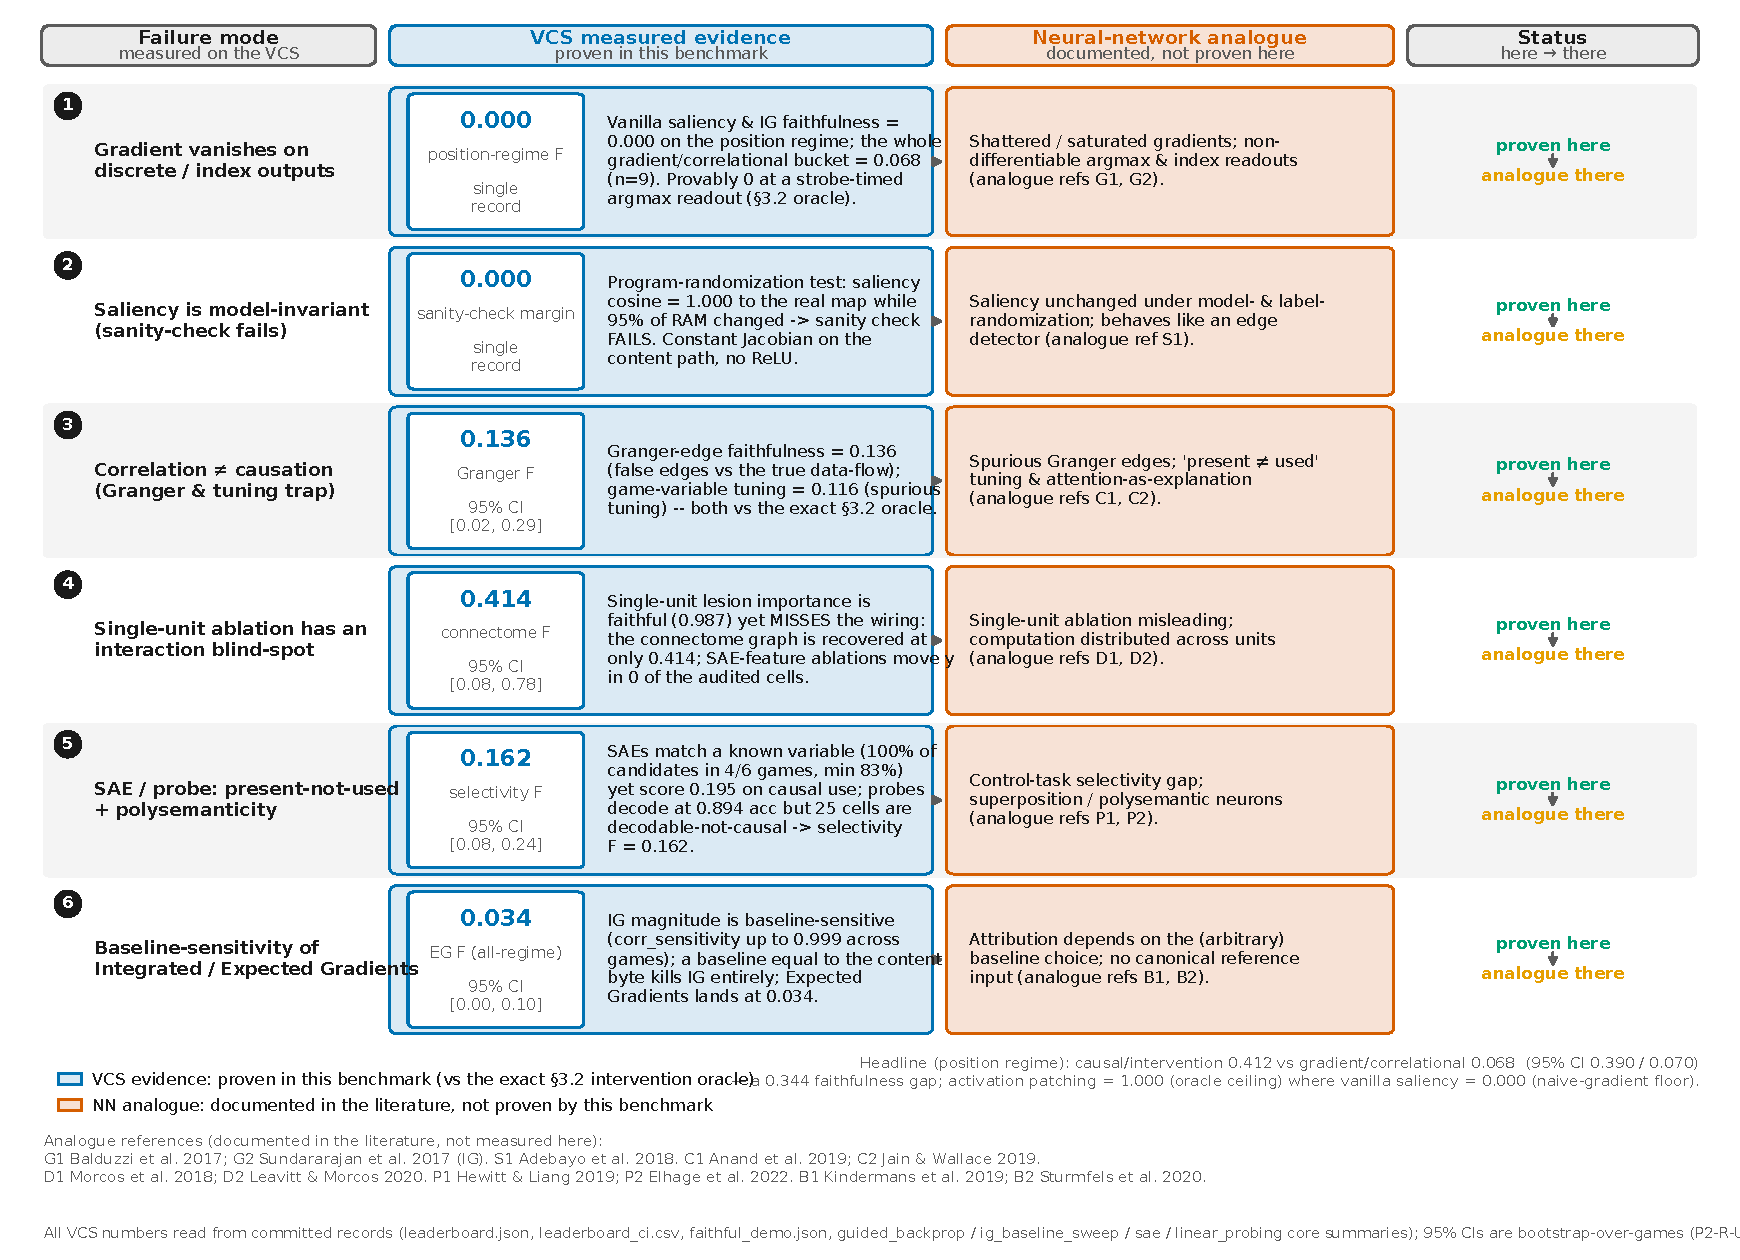
\includegraphics[width=\textwidth]{../figures/fig5_representativeness_map_full.pdf}
\caption{\textbf{Full VCS-to-NN representativeness map.} The full-density version of the
main-text map (Fig.~\ref{fig:representativeness}): each VCS failure mode is placed against its documented
neural-network analogue from the literature. The neural-network column records documented
analogues, not parallels proven by this benchmark; the oracle is the intervention oracle of
\Sectionname3.2, and the underlying per-method values trace to
\texttt{compare/out/leaderboard.json} via Sec.~\ref{supp:provenance}. Note that this full
map is the figure the simplified main-text version condenses.}
\label{supp:fig:repmap}
\end{figure}

\begin{figure}[t]
\centering
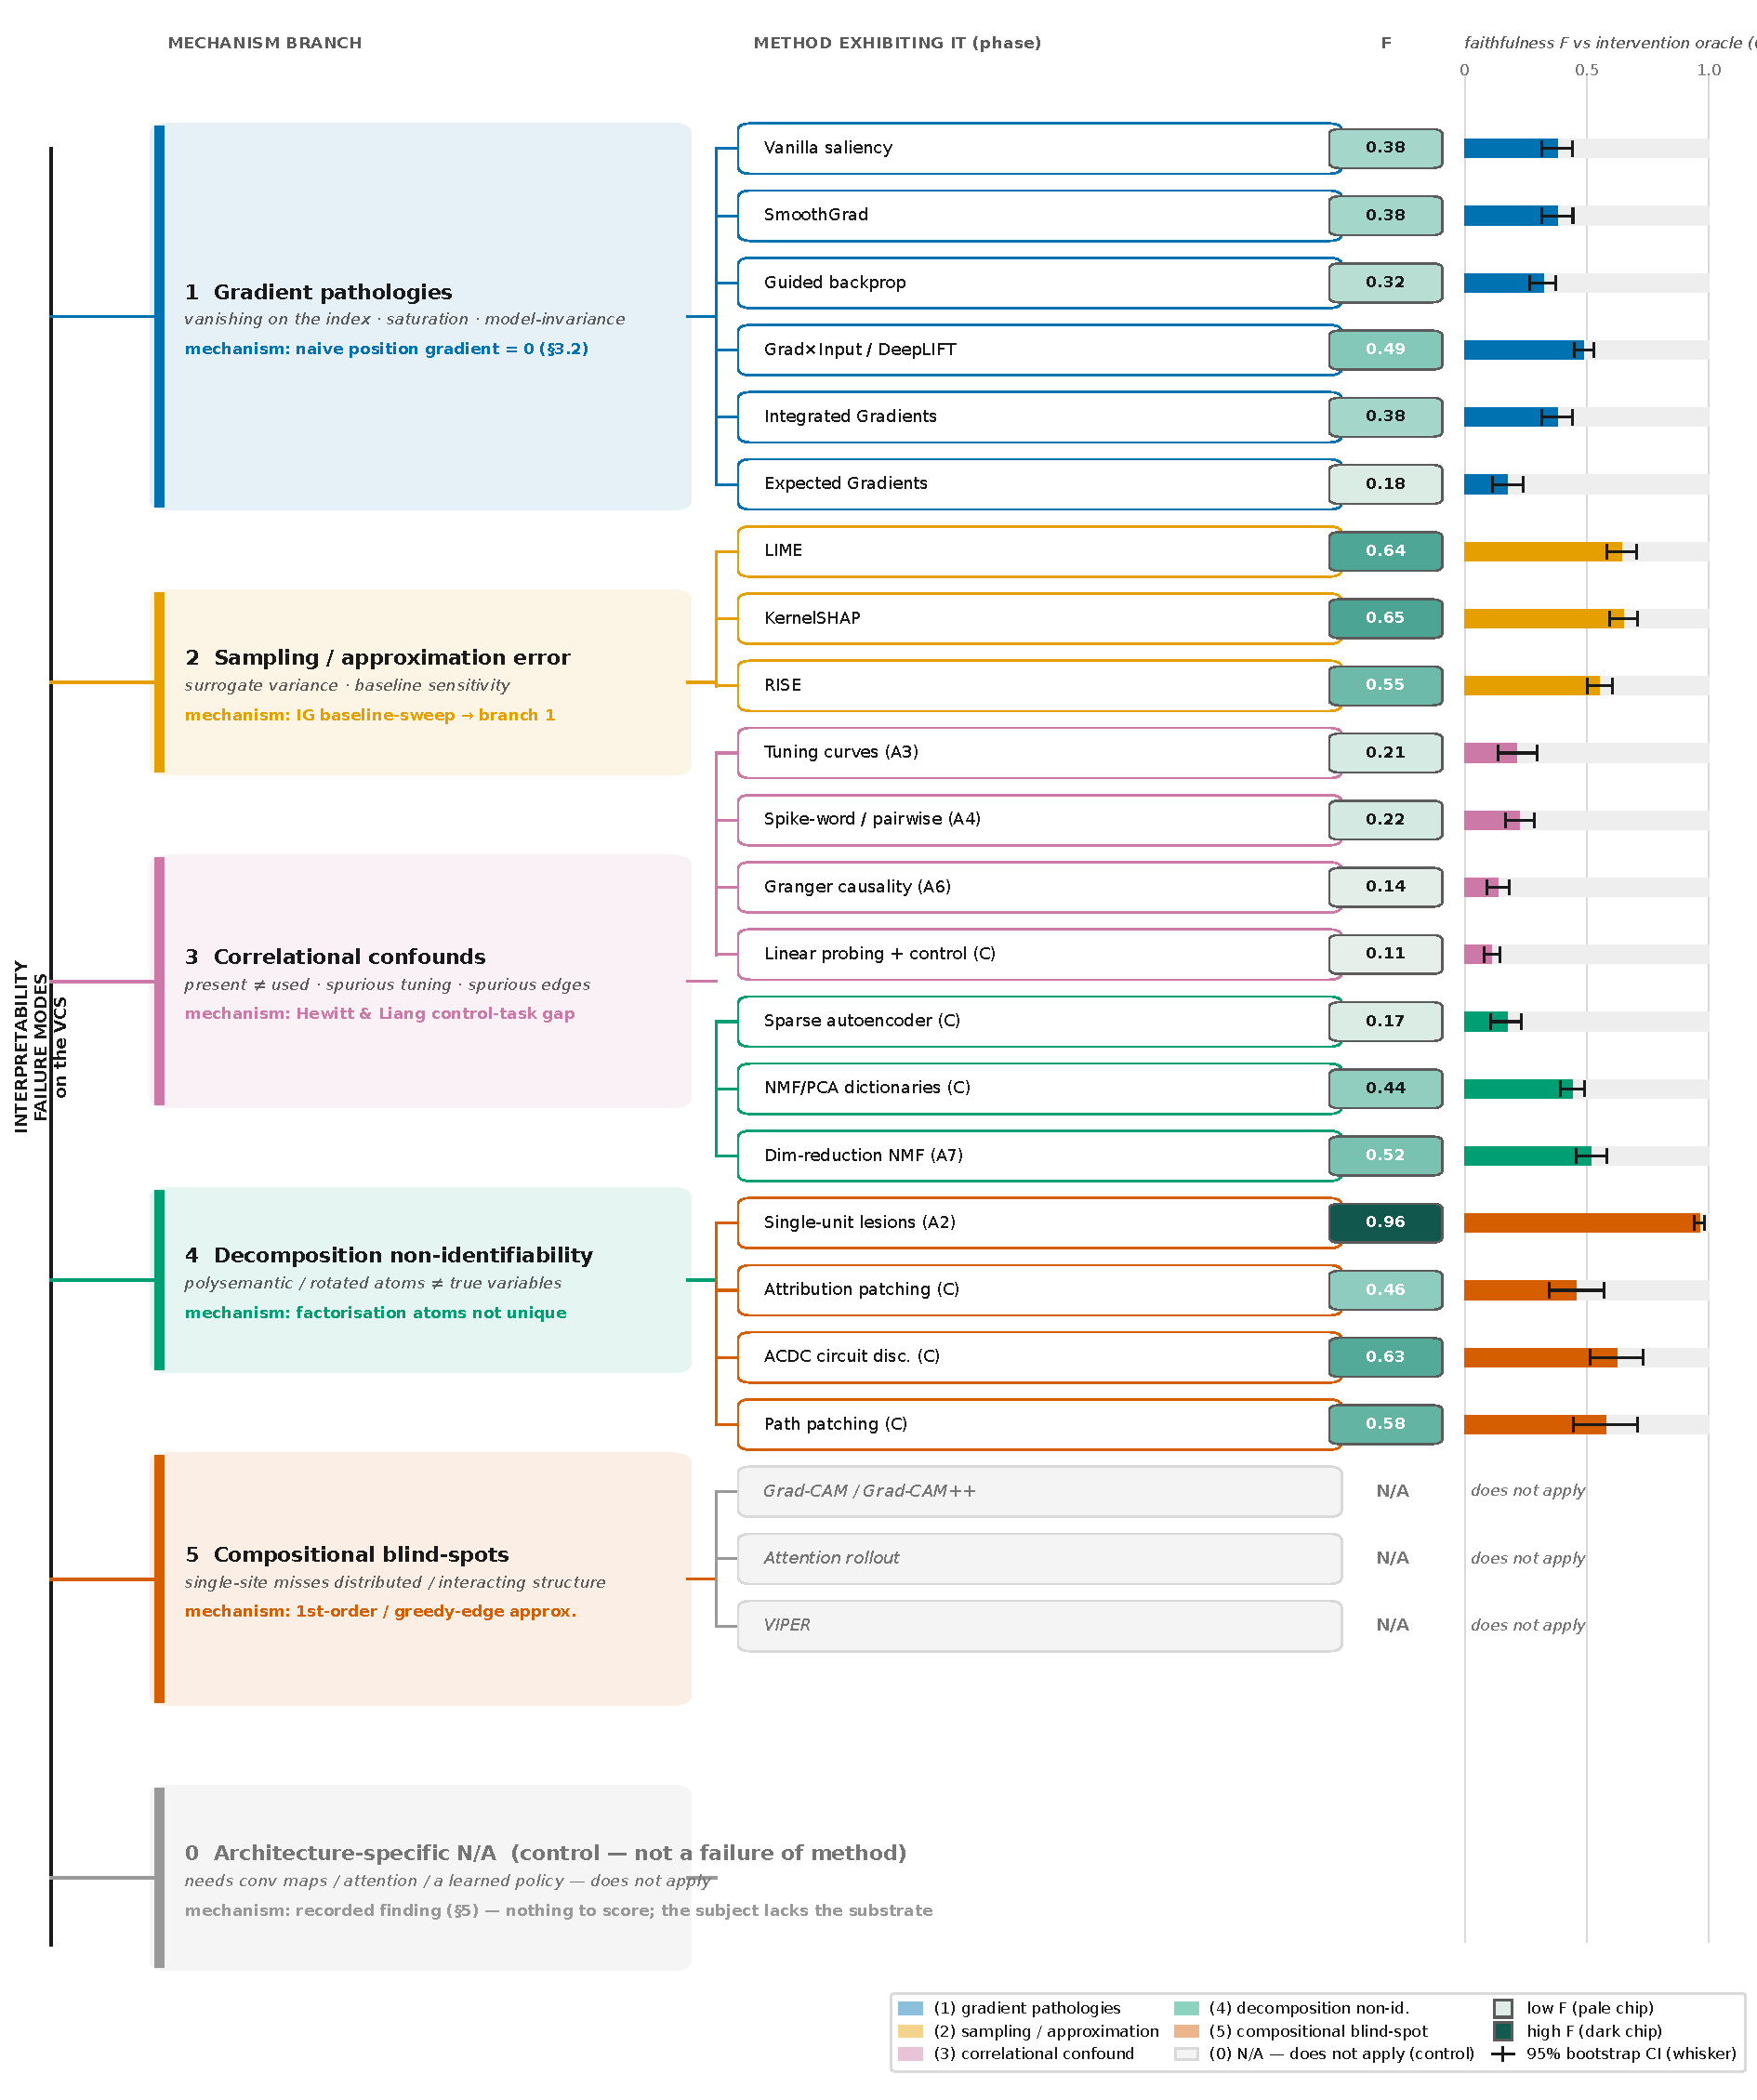
\includegraphics[width=\textwidth]{../figures/fig6_failure_taxonomy_full.pdf}
\caption{\textbf{Full failure taxonomy.} The full-density version of the main-text taxonomy
(Fig.~\ref{fig:taxonomy}): the families of interpretability failure observed on the machine, each annotated
with its faithfulness against the intervention oracle (\Sectionname3.2), reported as $F$ with its
$95\%$ bootstrap confidence interval. The leaf values trace to
\texttt{compare/out/leaderboard.json} and \texttt{leaderboard\_ci.csv} via
Sec.~\ref{supp:provenance}. Note that the gradient and correlational branches collapse on
the discrete position regime, where the naive gradient is provably zero (Prop.~\ref{prop:zero}).}
\label{supp:fig:taxonomy}
\end{figure}

\section{Plausibility-proxy rubric and its sensitivity}\label{supp:plausibility}

The plausibility axis of the leaderboard is a documented, tradition-level proxy, not a
human-subjects measurement. This section records how each value was assigned. It also shows
that the headline contrast does not depend on the particular numbers chosen. The Methods
(\Sectionname\ref{sec:triad}) name two reporting axes. Faithfulness is measured on the machine against the
intervention oracle of \Sectionname\ref{sec:oracle}. The plausibility proxy stands in for how convincing a
tradition's explanations are usually taken to be. We assign the proxy once per method
tradition, before any faithfulness score on our machine is computed, so it cannot be tuned to
the result. Its only job is to expose the danger zone of explanations that look convincing yet
are unfaithful. For that job it must be coarse, fixed in advance, and sourced rather than
precise.

The rubric assigns one proxy per tradition on a fixed five-step scale. It scores two
documented properties of each tradition's typical output and takes their average. The first
property is whether the explanation produces a dense, picture-like artifact that a reader sees
as an account of the computation. Heatmaps and saliency-style maps over the input are read as
convincing by construction. This is the perceptual-immediacy axis. The second property is
whether the field has historically treated the tradition's output as a self-evident
explanation rather than a hypothesis to be tested. This is the adoption-as-explanation axis. A
tradition that scores high on both, such as gradient saliency, receives a high proxy. A
tradition whose output is an austere intervention table or a circuit edge list, rarely
mistaken for a finished story, receives a low one. The scale is deliberately blunt,
$\{0.3,0.5,0.55,0.75,0.8,0.85,0.9\}$. A proxy meant to expose a danger zone gains nothing from
false precision, and a finer scale would invite over-reading. Every value in
Table~\ref{supp:tab:plausrubric} traces to the \jkey{plausibility_proxy} field of the
per-method rows in \texttt{compare/out/leaderboard.json}. The table only groups those rows by
tradition and records the rationale.

\begin{table}[t]
\centering
\caption{\textbf{Plausibility-proxy rubric.} The proxy assigned to each method tradition,
with the documented rationale. Values are the \jkey{plausibility_proxy} field of the
leaderboard rows (\texttt{compare/out/leaderboard.json}). They are tradition-level and fixed
before any faithfulness score is computed, so the proxy cannot be tuned to the measured
faithfulness. A higher value means an explanation that the field tends to find more
convincing, not one that is more faithful. The oracle (\Sectionname\ref{sec:oracle}) is the positive control and
is not a method under test.}
\label{supp:tab:plausrubric}
\begin{tabular}{@{}llp{6.4cm}@{}}
\toprule
Tradition & Proxy & Rationale (documented basis) \\
\midrule
gradient        & $0.90$ & Dense input-space heatmaps read as a visual account of the
                            decision; the most widely adopted XAI outputs, routinely shown
                            as if self-explanatory. \\
probing         & $0.85$ & A trained decoder that ``finds'' a concept reads as evidence the
                            concept is used; high adoption, though decodability is not
                            causal use. \\
correlational   & $0.80$ & Tuning curves and coupling spectra match the neuroscience idiom
                            of a convincing single-unit account. \\
dim.\ reduction & $0.75$ & Low-dimensional factors and dictionary atoms look like a clean
                            summary of the representation. \\
intervention    & $0.55$ & Occlusion and counterfactual outputs are quantitative tables, less
                            immediately picture-like, treated as tests rather than stories. \\
causal          & $0.50$ & Circuit edge lists and patching results are austere artifacts
                            rarely mistaken for a finished narrative. \\
descriptive     & $0.30$ & Whole-state recording is an explicit non-explanation: it withholds
                            nothing and reads as a dump, not an account. \\
\midrule
oracle (control)& $1.00$ & The \Sectionname\ref{sec:oracle} ground truth by construction; positive control, not a
                            method under test. \\
\bottomrule
\end{tabular}
\end{table}

The paper draws a contrast between this proxy and measured faithfulness. On the committed
records the two move in opposite directions. Across the thirty methods under test the Spearman
rank correlation between faithfulness and the proxy is $-0.36$, a negative association.
The traditions the field finds most convincing are, on this machine, among the least faithful.
Eight methods fall in the danger zone, defined here as a proxy of at least $0.70$ together
with a faithfulness below $0.40$. They include the correlational neuroscience methods, Expected
Gradients, guided backprop, linear probing, and the sparse autoencoder. The per-method extreme
makes the point sharply. Vanilla saliency has the highest proxy, $0.9$, yet scores faithfulness
$0.115$ on the position regime. Activation patching has a lower proxy, $0.5$, and scores $1.0$.
Here the less faithful method is the more plausible one. These figures are produced by
\texttt{tools/xai\_study/compare/plausibility\_sensitivity.py} from the leaderboard and
recorded in \texttt{compare/out/plausibility\_sensitivity.csv}.

A proxy fixed by a coarse rubric raises the question of whether the contrast is an artifact of
the particular numbers. The answer is that it is not. We perturb the proxy under four
deterministic schemes and recompute the relationship each time. The analysis uses fixed,
index-keyed offsets rather than random draws, so it re-derives bit-for-bit. The first scheme
adds a fixed per-method jitter of magnitude $\sigma\in\{0.05,0.1,0.2\}$, alternating in sign by
row. The second compresses every proxy toward the common mean by a fraction $\sigma$, which
preserves the rank order of traditions. The third uses the same index-keyed offsets at
$\sigma\in\{0.1,0.2\}$, large enough to swap neighbouring traditions' ranks. The fourth drops
one whole tradition at a time and recomputes on the remainder. Across all fourteen
perturbations the rank correlation between faithfulness and proxy stays negative. It ranges
from $-0.76$ to $-0.08$. The danger zone stays populated, with
between four and ten methods. The per-method anchor sign holds in every scheme where both
anchor methods are present, the more plausible saliency remaining the less faithful. Two runs
bound the range. The strongest is the leave-the-gradient-tradition-out run. It removes the most
plausible and least faithful block at once, and still leaves six danger-zone methods and a rank
correlation of $-0.76$. The weakest is the leave-the-causal-tradition-out run, where the
correlation falls to $-0.08$, close to zero; removing the faithful causal block flattens the
association, so the contrast is carried in part by that block. Table~\ref{supp:tab:plaussens}
reports the full sweep. The contrast keeps its sign under every alternative proxy assignment we
tried: plausibility and faithfulness are not the same axis, and high plausibility is no
guarantee of faithfulness.

\begin{table}[t]
\centering
\caption{\textbf{Proxy-sensitivity sweep.} The faithfulness-versus-proxy relationship under
each perturbation, from \texttt{compare/out/plausibility\_sensitivity.csv}. ``$\rho$'' is the
Spearman rank correlation between faithfulness and proxy over the methods present. ``danger''
is the count of high-proxy ($\geq0.70$), low-faithfulness ($<0.40$) methods. ``anchor'' is
$1$ when the more plausible saliency is the less faithful of the saliency/activation-patching
pair, and blank where a leave-one-out run removes an anchor. The baseline rubric is the first
row. Across every scheme the correlation stays negative and the danger zone stays populated.}
\label{supp:tab:plaussens}
\begin{tabular}{@{}llrrrc@{}}
\toprule
Scheme & Param & $n$ & $\rho$ & Danger & Anchor \\
\midrule
baseline                & ---           & 30 & $-0.36$ &  8 & 1 \\
additive jitter         & $\sigma=0.05$ & 30 & $-0.40$ &  8 & 1 \\
additive jitter         & $\sigma=0.10$ & 30 & $-0.41$ &  8 & 1 \\
additive jitter         & $\sigma=0.20$ & 30 & $-0.42$ & 10 & 1 \\
rank-preserving         & $\sigma=0.10$ & 30 & $-0.36$ &  8 & 1 \\
rank-preserving         & $\sigma=0.20$ & 30 & $-0.36$ &  8 & 1 \\
rank-jittering          & $\sigma=0.10$ & 30 & $-0.41$ &  8 & 1 \\
rank-jittering          & $\sigma=0.20$ & 30 & $-0.42$ & 10 & 1 \\
leave-out causal        & ---           & 24 & $-0.08$ &  8 & \\
leave-out correlational & ---           & 26 & $-0.40$ &  4 & 1 \\
leave-out descriptive   & ---           & 29 & $-0.29$ &  8 & 1 \\
leave-out dim.\ red.    & ---           & 27 & $-0.34$ &  7 & 1 \\
leave-out gradient      & ---           & 20 & $-0.76$ &  6 & \\
leave-out intervention  & ---           & 25 & $-0.34$ &  8 & 1 \\
leave-out probing       & ---           & 29 & $-0.36$ &  7 & 1 \\
\bottomrule
\end{tabular}
\end{table}

; the tables
%% render without overfull boxes and the two SI figures resolve from ../figures/.

\clearpage
\appendix

%% Breakable monospaced JSON key: lets long under_scored keys wrap inside narrow table
%% columns. Used by S5 (number provenance). Defined here so the S-files stay self-contained.
\providecommand{\jkey}[1]{\texttt{\expandafter\jkeyaux#1\relax}}
\makeatletter
\def\jkeyaux#1{\ifx\relax#1\else
  \ifx_#1\discretionary{}{}{}\char`\_\else
    \ifx.#1\discretionary{}{}{}.\else#1\fi\fi
  \expandafter\jkeyaux\fi}
\makeatother

\section*{Supplementary Information}
\setcounter{table}{0}
\setcounter{figure}{0}
\renewcommand{\thetable}{S\arabic{table}}
\renewcommand{\thefigure}{S\arabic{figure}}
\renewcommand{\thesection}{S\arabic{section}}
\setcounter{section}{0}

This Supplementary Information records what the main paper summarizes. We give the
per-method protocols (\Sectionname\ref{supp:protocols}) and the leaderboard schema with its glossary
(\Sectionname\ref{supp:schema}). We give the coverage and applicability of every method across games
and output regimes (\Sectionname\ref{supp:coverage}). We map each headline claim to its evidence
(\Sectionname\ref{supp:claims}). We trace the provenance of every headline number down to the record
file and command that produced it (\Sectionname\ref{supp:provenance}). We state plainly what the
paper does not claim (\Sectionname\ref{supp:notclaimed}). We give the plausibility-proxy rubric and
its sensitivity analysis (\Sectionname\ref{supp:plausibility}). The main text shows simplified forms
of two diagnostic figures; we reproduce both here at full resolution
(Figs.~\ref{supp:fig:repmap} and~\ref{supp:fig:taxonomy}).
The correctness triad $\mathrm{F}\wedge\mathrm{S}\wedge\mathrm{M}$ used throughout is the
one defined in the main Methods (\Sectionname\ref{sec:triad}); we reference it here rather than restating it. The
benchmark scores 30 interpretability methods together with the intervention oracle (\Sectionname\ref{sec:oracle})
as a positive control, for 31 leaderboard rows in total.

\section{Per-method protocols}\label{supp:protocols}

This section records five things for each method under test. It records the exact objects the
method consumes and produces, the reference it is scored against, its sampling or optimization
budget, the metric that turns its output into a faithfulness score, and the committed record
file (version-controlled, in the released repository) that holds the per-game results. All methods share one evaluation contract. We state that
contract once and then specialize it per method. Every method receives the same bit-exact VCS
state on each game of the scored set. We state the contract on the six core games
(\texttt{breakout}, \texttt{ms\_pacman}, \texttt{pong}, \texttt{qbert}, \texttt{seaquest},
\texttt{space\_invaders}), which carry the full tiered ground truth and the exact oracle and
serve as the running example; the aggregate leaderboard scores extend the identical protocol
to the 42-game scored set of \Sectionname\ref{supp:scoredset}. That state is not the boot screen.
It is a shared gameplay state, produced by a single seeded random-action stream (seed~$0$) run
for a $90$-frame prefix and then rolled forward for a $15$-frame analysis horizon. The stream is
deterministic, so every method sees the identical state on each game, and the run is asserted
bit-exact per game. An oracle cause-density gate screens the state before any method runs. The
gate counts how many candidate causes move the output above a floor and rejects states with too
few, so a near-flat oracle column cannot pass. This gate is what turns a degenerate frame into a
usable one; on \texttt{seaquest} it raises the count of live candidate causes from $2$ to $19$.
The candidate-cause set is the machine's own state. This set is the RAM bytes together with the
CPU registers and the TIA and RIOT registers exposed by the substrate. The output every method
attributes over is a shared screen-buffer region read at the end of the analysis horizon, not a
single hand-picked pixel. The reference is the intervention oracle of \Sectionname\ref{sec:oracle},
evaluated by exact re-runs of the emulator under $\mathrm{do}(u)$. A method that
cannot be applied to a given output regime is recorded as not-applicable rather than scored
as zero. An empty result is therefore never read as a wrong one. Faithfulness is the F
axis of the main-text triad (\Sectionname\ref{sec:triad}); we reference that definition and do not restate it.
Records live under \texttt{tools/xai\_study/<phase>/out/}; the aggregate they feed is
\texttt{tools/xai\_study/compare/out/leaderboard.json}.
Table~\ref{supp:leaderboard} consolidates the triad scores for all thirty methods and the
oracle positive control in one place; the per-method protocols follow.

\begin{table*}[t]
\centering
\caption{\textbf{Consolidated leaderboard: all methods, all triad axes.} One row per method
across the three phases, plus the intervention oracle as a positive control. $F$ is
faithfulness (Pearson correlation against the oracle, with the bootstrap-over-games 95\% CI in
brackets), $S$ is sufficiency, $M$ is minimality, all as defined in \Sectionname\ref{sec:triad};
Plaus is the elicited plausibility prior and $n$ is the number of scored games. Attribution
methods that emit only a saliency have no defined $S$ or $M$ and are marked ``---''; A5
(field potentials) and A7 (dimensionality reduction) likewise lack the $S$/$M$ decomposition.
Values are transcribed from \texttt{tools/xai\_study/compare/out/leaderboard.json} (the
committed numbers of record).}
\label{supp:leaderboard}
\footnotesize
\setlength{\tabcolsep}{4pt}
\begin{tabularx}{\textwidth}{@{}Xccccccc@{}}
\toprule
Method & Phase & Tradition & $F$ (95\% CI) & $S$ & $M$ & Plaus & $n$ \\
\midrule
A1 connectomics & A & intervention & 0.207 [0.130, 0.293] & 0.971 & 0.967 & 0.55 & 35 \\
A2 lesions & A & intervention & 0.965 [0.942, 0.983] & 0.591 & 1.000 & 0.55 & 42 \\
A3 tuning curves & A & correlational & 0.213 [0.136, 0.295] & 0.200 & 0.928 & 0.80 & 42 \\
A4 spike-word / pairwise & A & correlational & 0.225 [0.166, 0.283] & 0.133 & 0.363 & 0.80 & 34 \\
A5 field potentials & A & correlational & 0.376 [0.323, 0.428] & --- & --- & 0.80 & 40 \\
A6 Granger & A & correlational & 0.136 [0.091, 0.184] & 0.884 & 0.647 & 0.80 & 35 \\
A7 dim.\ reduction & A & dim.\ red. & 0.519 [0.457, 0.581] & --- & --- & 0.75 & 42 \\
A8 whole-state & A & descriptive & 1.000 [1.000, 1.000] & 1.000 & 0.075 & 0.30 & 42 \\
\midrule
Vanilla saliency & B & gradient & 0.380 [0.316, 0.445] & --- & --- & 0.90 & 42 \\
smoothgrad & B & gradient & 0.380 [0.317, 0.445] & --- & --- & 0.90 & 42 \\
Guided backprop & B & gradient & 0.322 [0.267, 0.375] & --- & --- & 0.90 & 42 \\
Grad$\times$Input / DeepLIFT & B & gradient & 0.486 [0.448, 0.526] & --- & --- & 0.90 & 42 \\
Integrated Gradients & B & gradient & 0.379 [0.314, 0.444] & --- & --- & 0.90 & 42 \\
Expected Gradients & B & gradient & 0.175 [0.110, 0.240] & --- & --- & 0.90 & 42 \\
kernelshap & B & gradient & 0.652 [0.596, 0.709] & --- & --- & 0.90 & 42 \\
lime & B & gradient & 0.644 [0.582, 0.705] & --- & --- & 0.90 & 42 \\
rise & B & gradient & 0.552 [0.500, 0.600] & --- & --- & 0.90 & 42 \\
occlusion & B & intervention & 0.687 [0.624, 0.746] & --- & --- & 0.55 & 42 \\
Extremal perturbation & B & intervention & 0.461 [0.410, 0.513] & --- & --- & 0.55 & 42 \\
On-distribution counterfactual & B & intervention & 0.433 [0.343, 0.522] & --- & --- & 0.55 & 42 \\
\midrule
Activation patching & C & causal & 1.000 [1.000, 1.000] & --- & --- & 0.50 & 42 \\
Causal scrubbing & C & causal & 0.979 [0.940, 1.000] & 0.979 & 0.814 & 0.50 & 42 \\
Interchange interventions (DAS) & C & causal & 1.000 [1.000, 1.000] & --- & --- & 0.50 & 42 \\
Logit / tuned lens & C & causal & 0.820 [0.768, 0.871] & --- & 0.224 & 0.50 & 42 \\
Path patching & C & causal & 0.580 [0.452, 0.710] & --- & --- & 0.50 & 42 \\
ACDC & C & causal & 0.625 [0.514, 0.730] & 0.299 & 1.000 & 0.50 & 35 \\
Attribution patching & C & gradient & 0.456 [0.345, 0.573] & --- & --- & 0.90 & 42 \\
Linear probing (+ control) & C & probing & 0.240 [0.153, 0.346] & --- & 0.932 & 0.85 & 42 \\
NMF / PCA dictionaries & C & dim.\ red. & 0.102 [0.049, 0.160] & 0.751 & 0.966 & 0.75 & 42 \\
Sparse autoencoder & C & dim.\ red. & 0.153 [0.096, 0.218] & 0.183 & 0.934 & 0.75 & 40 \\
\midrule
Intervention oracle & --- & oracle & 1.000 [1.000, 1.000] & 1.000 & 1.000 & 1.00 & 1 \\
\bottomrule
\end{tabularx}
\end{table*}

The neuroscience analyses (Phase~A) treat the running machine as a brain. It asks how far
each classical analysis recovers the known mechanism on the shared gameplay state. Each
method's baseline is the exact data-flow graph or causal role that the substrate makes
available. Its budget is the scored set (\Sectionname\ref{supp:scoredset}) unless noted,
with the six-game core as the running example, and its scoring metric is named in
Table~\ref{supp:tab:phaseA}. One core cell is honestly degenerate. On \texttt{ms\_pacman} the
pairwise analysis (A4) finds no coupled candidate pair to score at that frame, so its
\texttt{ms\_pacman} value is uninformative rather than a failure; the other five games carry
it.

\begin{table}[t]
\centering
\caption{\textbf{Phase~A protocols (neuroscience analyses).} One row per method. The columns
give the input it reads, the reference it is scored against, the sampling or intervention
budget, the scoring metric, and the committed record. All eight run on the scored set
(\Sectionname\ref{supp:scoredset}), with the six core games as the running example;
faithfulness is the F axis of \Sectionname\ref{sec:triad}. The whole-state recording (A8) is included as a
descriptive upper bound on coverage. Its faithfulness $F$ is trivial, so we read it for its
minimality $M$.}
\label{supp:tab:phaseA}
\scriptsize
\setlength{\tabcolsep}{4pt}
\begin{tabular}{@{}p{1.7cm}p{2.6cm}p{1.9cm}p{2.6cm}p{1.0cm}@{}}
\toprule
Method & Input / candidate causes & Reference & Scoring metric & Record \\
\midrule
A1 connectomics & RAM/register activity over trajectory & data-flow graph & data-flow graph $F_1$ vs.\ oracle & A1 \\
A2 lesions & single-cell knockouts via $\mathrm{do}(u)$ & true causal role & lesion-importance $\rho$ vs.\ role & A2 \\
A3 tuning curves & per-cell response vs.\ variable & variable coupling & $1-$ spurious-tuning rate & A3 \\
A4 spike-word / pairwise & pairwise cell correlations & true coupling & corr.\ $\rho$ vs.\ coupling & A4 \\
A5 field potentials & pooled-activity spectra & true causal share & $1-$ clock-explained var. & A5 \\
A6 Granger & directed lag structure & true data-flow & $1-$ false-edge rate & A6 \\
A7 dim.\ reduction & NMF/PCA over activity & known variables & NMF matched-component frac. & A7 \\
A8 whole-state & full state record & oracle decomp. & minimality $M$ vs.\ oracle & A8 \\
\bottomrule
\end{tabular}

\smallskip
\noindent\scriptsize Records: \texttt{tools/xai\_study/phaseA\_kording/out/A\{1..8\}\_*}; all
eight run on the 42-game scored set (\Sectionname\ref{supp:scoredset}), with the six core
games as the running example (\jkey{n_games} per method in \jkey{leaderboard.json}).
\end{table}

The attribution methods (Phase~B) run the everyday XAI toolbox over the same gameplay state.
These methods produce a real-valued saliency or attribution over the candidate-cause set.
We score that output by Pearson correlation against the oracle attribution. The gradient family
runs with the bilinear sub-pixel sampler turned on, so it is scored on a real position gradient
and not on the naive one. The naive gradient of the discrete position output is provably zero
(Prop.~\ref{prop:zero}); the sampler restores a finite gradient, but the restored gradient is
low and mixed in faithfulness rather than a fix. Expected Gradients draws its reference pool
from the states of the same seeded gameplay trajectory, not from a synthetic baseline. Two cells
are honestly degenerate and recorded as such. The on-distribution counterfactual returns a zero
delta on \texttt{space\_invaders}, \texttt{ms\_pacman}, and \texttt{qbert}, where its perturbation
does not move the shared output at that frame; those cells are marked not-valid rather than
scored. Expected Gradients scores low on the content regime of every game except \texttt{pong},
because the causal byte it should land on is static there. The budgets that matter are the
Monte-Carlo or perturbation counts of the sampling estimators, recorded per method in
Table~\ref{supp:tab:phaseB}. The seed-dispersion of the stochastic members is carried in
\texttt{leaderboard\_ci.csv} (\texttt{seed\_sd}, \texttt{seed\_sd\_source}) and reproduced
in \Sectionname\ref{supp:provenance}.

\begin{table}[t]
\centering
\caption{\textbf{Phase~B protocols (attribution methods).} Each method emits a saliency over
the candidate-cause set. We score it by Pearson correlation against the oracle attribution
(\Sectionname\ref{sec:oracle}). The reference is shared and the budget is the scored set of
\Sectionname\ref{supp:scoredset} (six core games as the running example). The budget column records the
sampling or perturbation count that drives each estimator. The seed column flags which
methods carry an independent-seed dispersion in \texttt{leaderboard\_ci.csv}.}
\label{supp:tab:phaseB}
\scriptsize
\setlength{\tabcolsep}{4pt}
\begin{tabular}{@{}p{2.9cm}p{1.75cm}p{4.3cm}p{1.15cm}@{}}
\toprule
Method & Tradition & Budget / hyperparameters & Seed sd \\
\midrule
Vanilla saliency & gradient & single backward pass & --- \\
smoothgrad & gradient & noise-averaged gradient; $\sigma$-robustness committed & 0.0 \\
Guided backprop & gradient & single guided pass & --- \\
Grad$\times$Input / DeepLIFT & gradient & DeepLIFT reference-difference & --- \\
Integrated Gradients & gradient & path integral, baseline = zero state & --- \\
Expected Gradients & gradient & expectation over baselines (refits) & yes \\
kernelshap & gradient & Monte-Carlo coalition sampling ($\propto 1/\sqrt{N}$) & 0.017 \\
lime & gradient & local linear fit, perturbation refits & 0.029 \\
rise & gradient & random-mask Monte-Carlo ($\propto 1/\sqrt{N}$) & 0.051 \\
occlusion & intervention & exhaustive single-cell masking & --- \\
Extremal perturbation & intervention & optimized mask, area-constrained & --- \\
On-distribution counterfactual & intervention & on-manifold $\mathrm{do}(u)$ resampling & --- \\
\bottomrule
\end{tabular}

\smallskip
\noindent\scriptsize Records: \texttt{tools/xai\_study/phaseB\_attribution/out/}; all twelve run
on the 42-game scored set (\Sectionname\ref{supp:scoredset}), six core games as the running
example, and are scored by Pearson correlation against the oracle (\Sectionname\ref{sec:oracle}). Seed
sd is the independent-seed dispersion from \texttt{leaderboard\_ci.csv}.
\end{table}

The mechanistic methods (Phase~C) are built to recover circuits. Each is scored
against the true data-flow or the exact recovered-minus-exact deviation. The causal members
of this phase are the ones that reach the oracle ceiling. We list their exact scoring metric
so that the ceiling is not read as a tautology. Each member is scored against the substrate's
known routine, and not against another method. Two members (NMF/PCA dictionaries and the
sparse autoencoder) are dimensionality-reduction methods carried here for comparison. The
sparse autoencoder has two aggregations that differ, which we reconcile in
\Sectionname\ref{supp:provenance}.

\begin{table}[t]
\centering
\caption{\textbf{Phase~C protocols (mechanistic methods).} Each method is scored against the
substrate's known circuit or the exact recovered-minus-exact deviation (\Sectionname\ref{sec:oracle}), and not
against another method. This is what keeps the oracle ceiling non-circular. The probing and
dictionary-learning members are included for comparison with the causal members.}
\label{supp:tab:phaseC}
\scriptsize
\setlength{\tabcolsep}{4pt}
\begin{tabular}{@{}p{3.4cm}p{1.4cm}p{5.2cm}@{}}
\toprule
Method & Tradition & Scoring metric \\
\midrule
Activation patching & causal & $\max|\text{recovered}-\text{exact}|$ vs.\ oracle \\
Causal scrubbing & causal & scrubbing-preserved performance \\
Interchange interventions (DAS) & causal & aligned interchange accuracy \\
Logit / tuned lens & causal & logit-lens fidelity to true intermediate \\
Path patching & causal & path-circuit $F_1$ vs.\ true routine \\
ACDC & causal & discovered-circuit best $F_1$ vs.\ data-flow \\
Attribution patching & gradient & corr.\ of approximation vs.\ exact patch \\
Linear probing (+ control) & probing & selectivity vs.\ control task \\
NMF / PCA dictionaries & dim.\ red. & matched-component fraction vs.\ vars \\
Sparse autoencoder & dim.\ red. & feature-variable matched fraction \\
\bottomrule
\end{tabular}

\smallskip
\noindent\scriptsize Records: \texttt{tools/xai\_study/phaseC\_mechanistic/out/}; all ten run
on the 42-game scored set (\Sectionname\ref{supp:scoredset}), with the six core games as the
running example.
\end{table}

The intervention oracle is the positive control, not a method under test. It is the exact
$\mathrm{do}(u)$ ground truth of \Sectionname\ref{sec:oracle}, evaluated by re-running the bit-exact machine. It
attains $F=S=M=1.0$ by construction. Its record triple is the intervention oracle, the
content-path gradient oracle, and their cross-check
(\texttt{tools/xai\_study/ground\_truth/out/}). It anchors the ceiling against which every
other row is read, which is why it occupies the thirty-first leaderboard row.

\section{Benchmark schema and glossary}\label{supp:schema}

The leaderboard is built from a flat record schema. Stating it removes the ambiguity
about what a single number on the benchmark counts. Each method is run per game and writes a
per-game record under its phase's \texttt{out/} tree. The leaderboard aggregates those
records into one row per method by averaging over games. The schema columns of a leaderboard
row are given in Table~\ref{supp:tab:schema}. The aggregation rule is a mean over the
$n_{\text{games}}$ games. When a method emits several output records on one game, those records
are first reduced within that game. The faithfulness, sufficiency, and minimality columns
report the F, S, and M axes defined in \Sectionname\ref{sec:triad}. We do not re-derive those definitions here.

\begin{table}[t]
\centering
\caption{\textbf{Leaderboard row schema.} The columns of one row in
\texttt{compare/out/leaderboard.json} (\texttt{rows[\,]}) and its uncertainty companion
\texttt{leaderboard\_ci.csv}. The metric column names the per-method scoring function from
\Sectionname\ref{supp:protocols}; F, S, and M are the triad axes of \Sectionname\ref{sec:triad}. Aggregation is a mean
over $n_{\text{games}}$, with bootstrap confidence intervals over games (and, where present,
over records).}
\label{supp:tab:schema}
\footnotesize
\begin{tabular}{@{}p{3.0cm}p{8.4cm}@{}}
\toprule
Column & Meaning \\
\midrule
\texttt{phase} & phaseA\_kording, phaseB\_attribution, phaseC\_mechanistic, or ground\_truth \\
\texttt{method} & method identifier (the row key) \\
\texttt{tradition} & intervention, causal, gradient, correlational, \jkey{dim_reduction}, probing, descriptive, oracle \\
\jkey{n_games} & number of games the method was scored on (up to 42 for the scored set of \Sectionname\ref{supp:scoredset}; 1 for the oracle) \\
\jkey{n_records} & number of per-game output records aggregated into the row \\
\texttt{faithfulness} (F) & faithfulness vs.\ the intervention oracle (\Sectionname\ref{sec:oracle}), $[0,1]$, higher better \\
\jkey{faithfulness_ci95} & $95\%$ bootstrap CI half-width over games \\
\jkey{faithfulness_position_regime} & F restricted to the discrete sprite-position/index regime \\
\jkey{faithfulness_content_regime} & F restricted to the continuous content regime \\
\texttt{triad\_S} / \texttt{triad\_M} & sufficiency / minimality axes (\Sectionname\ref{sec:triad}), where applicable \\
\jkey{plausibility_proxy} & documented method-tradition proxy, $[0,1]$ --- not a human-subjects measurement \\
\jkey{is_positive_control} & 1 for the oracle row, 0 otherwise \\
\jkey{metric_names} & the per-method scoring function (\Sectionname\ref{supp:protocols}) \\
\texttt{commits} & the commit(s) at which the per-game records were produced \\
\bottomrule
\end{tabular}
\end{table}

We fix the vocabulary that the schema implies, because the review asked for a single
unambiguous method count. A \emph{method} is one interpretability technique, e.g.\
\texttt{vanilla\_saliency}. A \emph{method row} is its single aggregated line on the
leaderboard. A \emph{per-game record} is one method scored on one game, written under a phase
\texttt{out/} tree. An \emph{output record} is a per-game record for one output regime; a
method may emit several of these on one game. A \emph{family mean} is the average over the
members of a tradition family, e.g.\ causal/intervention. The \emph{oracle positive control}
is the exact $\mathrm{do}(u)$ ground truth of \Sectionname\ref{sec:oracle}, scored as a method to anchor the
ceiling. A \emph{not-applicable method} is one that does not apply to a given output regime;
it is recorded as N/A rather than as a zero. With this vocabulary the count is unambiguous.
The benchmark scores 30 interpretability methods together with the intervention
oracle as a positive control, for 31 leaderboard rows in total
(\texttt{leaderboard.json.n\_methods}~$=31$), aggregating 1773 per-game records over the
42-game scored set (\texttt{n\_per\_game\_records\_aggregated}~$=1773$): 8 methods in
Phase~A, 12 in Phase~B, 10 in Phase~C, and the one oracle row. This count is the canonical one
used in the abstract, the figures, and throughout this Supplement.

\section{Coverage and applicability}\label{supp:coverage}

The benchmark scores methods on a six-game core drawn from a larger bit-exact substrate. The
coverage table makes the scope of that choice explicit. Paper~1 validates the
differentiable VCS ports bit-for-bit against the \texttt{xitari} reference on all 64 Arcade
Learning Environment games, within a 30-frame RAM and 60-frame screen window. The
interpretability study reported here runs on the six games listed in
Table~\ref{supp:tab:coverage}. Every method is scored on a shared gameplay state, produced by
one seeded random-action stream (seed~$0$, $90$-frame prefix, $15$-frame analysis horizon), not
on the boot screen. This keeps the analysis inside the Paper~1 bit-exact window while giving the
oracle a rich, non-degenerate cause set to score against. We pick these six games because all
three tiers of ground truth (\Sectionname\ref{sec:tiers}) are available for them and the oracle is
exact. The remaining 58 games are
bit-exact substrate but are not scored here. Some fall outside the validated horizon for the
analyses we run. For others, the tiered labels they would need are not yet produced. They are
candidates for the larger sweep, and are not excluded for any methodological reason. The
horizon column records the validated window. The tier column records which of the three
ground-truth tiers (T1 exact intervention, T2 data-flow, T3 externally-supplied semantic
labels) is available.

\begin{table}[t]
\centering
\caption{\textbf{Core-game coverage.} The six core games carry exact tiered ground truth and
the full method battery. Faithfulness is scored within the Paper~1 bit-exact window. The
last two columns give the methods run and the per-game output records contributed. The wider
64-game substrate is bit-exact (Paper~1) but is reserved for the larger sweep. T3 labels are
external (\Sectionname\ref{sec:tiers}); we record this so the benchmark does not appear to certify them.}
\label{supp:tab:coverage}
\footnotesize
\setlength{\tabcolsep}{4pt}
\begin{tabular}{@{}p{2.4cm}p{1.9cm}p{1.5cm}p{1.7cm}p{1.5cm}p{1.4cm}@{}}
\toprule
Game & Paper-1 status & Horizon & Tiers & Methods run & Records \\
\midrule
breakout & bit-exact & 30/60 fr & T1,T2,T3 & 30 + oracle & per-game \\
ms\_pacman & bit-exact & 30/60 fr & T1,T2,T3 & 30 + oracle & per-game \\
pong & bit-exact & 30/60 fr & T1,T2,T3 & 30 + oracle & per-game \\
qbert & bit-exact & 30/60 fr & T1,T2,T3 & 30 + oracle & per-game \\
seaquest & bit-exact & 30/60 fr & T1,T2,T3 & 30 + oracle & per-game \\
space\_invaders & bit-exact & 30/60 fr & T1,T2,T3 & 30 + oracle & per-game \\
\midrule
58 further games & bit-exact (P1) & 30/60 fr & T1,T2 partial & reserved & --- \\
\bottomrule
\end{tabular}
\end{table}

A gameplay state can still be degenerate for a particular method, and the benchmark records
this rather than scoring it as a failure. The oracle cause-density gate is the first guard. It
counts how many candidate causes move the shared output above a floor, and rejects a state that
does not clear a minimum count, so a near-flat oracle column never reaches a method. On
\texttt{seaquest} the gate raises the count of live candidate causes at the analysis frame from
$2$ to $19$, which is what makes the game usable. Three residual degenerate cells survive the
gate and are marked, not scored as zero. On \texttt{ms\_pacman} the pairwise neuroscience
analysis (A4) finds no coupled candidate pair at that frame, so its cell is uninformative. The
on-distribution counterfactual returns a zero delta on \texttt{space\_invaders},
\texttt{ms\_pacman}, and \texttt{qbert}, where its perturbation does not move the shared output;
those cells are recorded as not-valid. Expected Gradients scores low on the content regime of
every game but \texttt{pong}, because the causal byte it should attribute to is static there.
None of these cells is read as a wrong answer.

Whether a method applies at all depends on what the method needs from its target. The
applicability matrix records that for every method family. The Phase~A neuroscience analyses
read the raw machine state and need neither a learned policy nor gradients. The Phase~B
attribution methods split into two groups. The gradient members need a differentiable forward
pass. The intervention members need only the ability to set state. The Phase~C mechanistic
methods need access to internal activations. The causal members among them also need the
ability to intervene. Table~\ref{supp:tab:applic} records, per family, whether the method
operates on the raw VCS, whether it requires a learned policy, gradients, internal layers or
attention, or external labels, whether it uses oracle-like interventions, and whether it
receives a supplied hypothesis. The table shows the same pattern the results confirm. The
families that score high on faithfulness are the ones that can intervene. The families that
collapse on the position regime are the gradient and correlational ones.

\begin{table}[t]
\centering
\caption{\textbf{Per-family applicability.} What each method family requires of its target.
``Intervenes'' marks oracle-like $\mathrm{do}(u)$ access; ``hypothesis'' marks methods that
receive a supplied circuit hypothesis to test. The raw-VCS column distinguishes analyses that
read machine state directly from those that need a differentiable or layered model. A blank
means the requirement does not apply.}
\label{supp:tab:applic}
\footnotesize
\begin{tabular}{@{}p{3.0cm}cccccc@{}}
\toprule
Family & raw VCS & policy & gradients & layers/attn & intervenes & hypothesis \\
\midrule
A neuroscience & yes & no & no & no & A2 only & no \\
B gradient & yes & no & yes & no & no & no \\
B intervention & yes & no & no & no & yes & no \\
C causal & yes & no & no & yes & yes & yes \\
C gradient (attr.\ patch) & yes & no & yes & yes & approx. & yes \\
C probing & yes & no & no & yes & no & no \\
C / A dim.\ reduction & yes & no & no & yes & no & no \\
oracle (control) & yes & no & no & yes & exact & --- \\
\bottomrule
\end{tabular}
\end{table}

\section{Claims and evidence}\label{supp:claims}

Every headline claim in the paper rests on a specific artifact. The table in this section
makes that dependency checkable. For each claim we list the figure or table that supports it,
the games and methods it uses, the metric, the artifact it traces to, and the limitation that
bounds it. Faithfulness, sufficiency, and minimality are the three axes of \Sectionname\ref{sec:triad}.
The numbers themselves are sourced in \Sectionname\ref{supp:provenance}. The table below names which
evidence supports which claim; it does not repeat the values. One split matters for how the
table is read. The all-regime faithfulness gap between causal/intervention and
gradient/correlational methods is $0.297$ with a $95\%$ interval of $[0.232,0.375]$ that
excludes zero, and it is the primary evidence for the headline. The position-only gap is
$0.238$ with an interval of $[-0.049,0.315]$ that crosses zero at six games. We report the
position gap as directional support, not as a significant result.

\begin{table}[t]
\centering
\caption{\textbf{Claims and their evidence.} Each headline claim maps to the figure or table
that supports it, the games and methods involved, the metric, the committed artifact, and the
limitation that bounds the claim. The artifact column points to the record that
\Sectionname\ref{supp:provenance} traces to a value. The limitation column states the scope, so the
claim is not read wider than the evidence.}
\label{supp:tab:claims}
\scriptsize
\setlength{\tabcolsep}{4pt}
\begin{tabular}{@{}p{3.0cm}p{1.9cm}p{1.8cm}p{1.9cm}p{2.4cm}@{}}
\toprule
Claim & Evidence & Methods / games & Metric & Limitation \\
\midrule
Causal/intervention methods beat gradient/correlational on faithfulness across all regimes & Fig.~\ref{fig:faithfulness}; leaderboard & 25 methods, 6 games & F mean (gap $0.297$) & robust: gap $0.297$ $[0.232,0.375]$ excludes zero; this all-regime gap is the primary evidence \\
The gap holds with the same sign on the discrete position regime & Fig.~\ref{fig:faithfulness}; \jkey{faithful_demo} & 13 rows, 6 games & F position (gap $0.238$) & directional only: gap $0.238$ $[-0.049,0.315]$ crosses zero at 6 games, so it is not significant \\
A faithful causal method reaches the oracle ceiling where the default tool stays low & \jkey{faithful_demo}; Fig.~\ref{fig:faithfulness} & act.\ patching vs.\ vanilla saliency, 6 games & F $1.0$ vs.\ $0.165$ (position regime; all-regimes saliency F $0.419$, plotted in Fig.~\ref{fig:faithfulness}) & one decisive pair \\
The naive gradient of a discrete position output is provably zero & Prop.~\ref{prop:zero} (\Sectionname\ref{sec:oracle}); \jkey{oracle_grad} & all gradient methods & grad@position $=0$; sampler restores $166$ & position path only; restored gradient is low/mixed \\
High plausibility coexists with low faithfulness (the danger zone) & Fig.~\ref{fig:faithfulness}; \jkey{faithful_demo} & vanilla saliency & proxy $0.9$, F $0.165$ (position regime; all-regimes F $0.419$, plotted in Fig.~\ref{fig:faithfulness}) & proxy, not measured plausibility \\
Faithful attribution recovers the wiring but not the computation's semantics & Fig.~\ref{fig:taxonomy} (\Sectionname\ref{supp:coverage}); discussion & Phase~B vs.\ C & F vs.\ S, M & necessary-condition stress test \\
The failure modes have documented NN analogues & Fig.~\ref{fig:representativeness} & taxonomy & --- & analogues, not proof \\
\bottomrule
\end{tabular}
\end{table}

\section{Number provenance}\label{supp:provenance}

Every headline number traces to a committed record, the script that produced it, and the
command that re-derives it. This section is the in-paper copy of that traceability table. It
mirrors \Sectionname6.5 of the reproducibility document
(\texttt{xai\_2\_interpretability/REPRODUCIBILITY.md}). The values are the measured, committed
ones at the current revision. The position-regime gap and its $95\%$ interval are read from
\texttt{tools/xai\_study/compare/out/position\_bootstrap.json}; the other aggregates from
\texttt{leaderboard.json}, rather than recomputed here. Each
record also carries \texttt{seed}, \texttt{where}, \texttt{commit}, and \texttt{timestamp}, so
the provenance of every value is self-documenting. The aggregate scores below are taken over
the 42-game scored battery of \Sectionname\ref{supp:scoredbattery}, not the six-game core;
each per-method row is a mean over the games on which that method applies (\jkey{n_games}
per method, e.g.\ 42 for most methods, 35 for ACDC and A1). The position-regime gap is now
significant on this battery.

\begin{table}[t]
\centering
\caption{\textbf{Headline-number provenance.} Each number $\rightarrow$ its committed record
and JSON key $\rightarrow$ the generating or aggregating script $\rightarrow$ the command
that reproduces it. Values are the measured, committed numbers at this revision (consistent
with REPRODUCIBILITY \Sectionname6.5); the position-regime gap CI is read from
\jkey{position_bootstrap.json}, all other aggregates from \jkey{leaderboard.json}. Paths are
relative to \texttt{tools/xai\_study/}.}
\label{supp:tab:provenance}
\scriptsize
\setlength{\tabcolsep}{3pt}
\renewcommand{\arraystretch}{1.15}
\begin{tabular}{@{}p{2.5cm}p{1.6cm}p{3.4cm}p{1.9cm}@{}}
\toprule
Number & Value & Record (JSON key) & Command \\
\midrule
Faithfulness gap, all regimes (causal $-$ gradient) & $0.3374$\newline {\scriptsize$[0.3103,0.3643]$, excl.\ $0$} & \jkey{position_bootstrap.json}: \jkey{all\_regime.family\_mean\_gap}, \jkey{ci95} & \jkey{position_bootstrap.py} \\
Causal/interv.\ mean F, all regimes & $0.7215$\newline {\scriptsize$n{=}11$} & \jkey{leaderboard.json}: \jkey{family_causal_intervention} \jkey{mean} & \jkey{leaderboard.py} \\
Gradient/corr.\ mean F, all regimes & $0.384$\newline {\scriptsize$n{=}14$} & \jkey{leaderboard.json}: \jkey{family_gradient_correlational} \jkey{mean} & \jkey{leaderboard.py} \\
Faithfulness gap, position regime (bootstrap over games) & $0.3268$\newline {\scriptsize$[0.1325,0.3702]$, excl.\ $0$} & \jkey{position_bootstrap.json}: \jkey{family_mean_gap}, \jkey{ci95} & \jkey{position_bootstrap.py} \\
Causal/interv.\ mean F, position regime & $0.561$\newline {\scriptsize$\pm0.3212$, $n{=}4$} & \jkey{leaderboard.json}: \jkey{family_..._intervention_position} \jkey{mean} & \jkey{leaderboard.py} \\
Gradient/corr.\ mean F, position regime & $0.2343$\newline {\scriptsize$\pm0.156$, $n{=}9$} & \jkey{leaderboard.json}: \jkey{family_..._correlational_position} \jkey{mean} & \jkey{leaderboard.py} \\
Decisive pair, position regime (act.\ patch vs.\ vanilla sal.) & $1.000$\newline vs.\ $0.115$ & \texttt{faithful\_demo}: \jkey{pair_contrast} & \jkey{faithful_demo.py} \\
Plausibility proxy, decisive pair & $0.5$ vs.\ $0.9$ & \texttt{faithful\_demo}: \jkey{...plausibility_proxy} & \jkey{faithful_demo.py} \\
ACDC sufficiency $S$ & $0.299$ & \jkey{leaderboard.json}: ACDC \jkey{triad_S} & \jkey{leaderboard.py} \\
Whole-state minimality $M$ & $0.0755$ & \jkey{leaderboard.json}: A8 \jkey{triad_M} & \jkey{leaderboard.py} \\
Methods scored (rows) & $31$ & \texttt{leaderboard}: \jkey{n_methods} & \jkey{leaderboard.py} \\
Per-game records aggregated & $1773$ & \texttt{leaderboard}: \jkey{n_per_game_records_aggregated} & \jkey{leaderboard.py} \\
Naive gradient, discrete position output & position $0$;\newline content $1.0$; sampler $166$ & \jkey{oracle_grad_pong.json}: \texttt{value}, \jkey{extra.sampler} & \jkey{oracle_grad.jl} \\
Exact oracle $\max|\Delta\text{score}|$ (Pong) & $17.0$ & \jkey{oracle_pong_score.json}: \texttt{value} & \jkey{oracle_intervene.jl} \\
\bottomrule
\end{tabular}

\smallskip
\noindent\scriptsize Scripts live under \texttt{tools/xai\_study/compare/} (Python) and
\texttt{tools/xai\_study/ground\_truth/} (Julia); records under the corresponding \texttt{out/}
trees. JSON keys are abbreviated with ``\texttt{...}'' where nested; the full paths are in
REPRODUCIBILITY \Sectionname6.5.
\end{table}

One number needs a reconciliation, and we record it rather than hide it. The sparse
autoencoder is the only method whose two aggregations disagree. On the 42-game scored battery
the over-games mean is $F=0.1526$ (\jkey{triad_F}) and the over-records mean is $0.1733$
(\jkey{faithfulness}); both are read from the sparse-autoencoder row of
\jkey{leaderboard.json}. The figures and the main-text leaderboard plot the over-records value
$0.1733$. We treat the over-games mean as the canonical row value for the aggregation rule of
\Sectionname\ref{supp:schema}, and report the over-records figure alongside it, so that text,
table, and figure agree on which aggregation each cites. No headline claim depends on which of
the two is read, since the sparse autoencoder sits near the floor under both.

\section{What this paper does not claim}\label{supp:notclaimed}

The benchmark is sharp precisely because its scope is narrow, and stating the boundaries
keeps the result from being read wider than the evidence carries it. We do not claim to
recover a program's semantics from scratch. The study measures whether an explanation names
the true causes and regenerates the behavior on a machine whose answer is already known; it
does not show that any method discovers the meaning of a routine without that ground truth in
hand, and the residual that faithfulness alone leaves behind, the gap between the wiring and
the computation, is the point rather than a result to be explained away.

We do not evaluate learned agents. The subject throughout is the bit-exact VCS itself, and
the candidate causes are its registers, RAM cells, and program variables, not the weights of
a trained policy. The neural-network parallels drawn in the discussion and in
Fig.~\ref{supp:fig:repmap} are documented analogues from the literature, not claims proven on
this benchmark; we label them as such so that a reader does not take a mapped failure mode
for a demonstrated one.

We do not prove that neural-network interpretability is impossible. The VCS gap is a
necessary-condition stress test: a method that fails to recover the wiring of a fully known
machine cannot be trusted to recover it on an unknown one, but a method that succeeds here is
not thereby certified on networks. The ``floor'' framing is an evidence-transfer argument,
not a proven lower bound on neural-network interpretability.

We do not measure human plausibility. The plausibility axis is a documented
method-tradition proxy, computed from a fixed rubric rather than collected from raters, and
we report it as a proxy throughout; its job is to expose the danger zone where a convincing
explanation is unfaithful, not to stand in for a human-subjects study. We also do not
redistribute the ROMs: the substrate is validated against an external reference, the records
are reproducible from committed artifacts without the ROMs, and the ROM provenance is given
as hashes so a third party supplies their own legally obtained copies.

\begin{figure}[t]
\centering
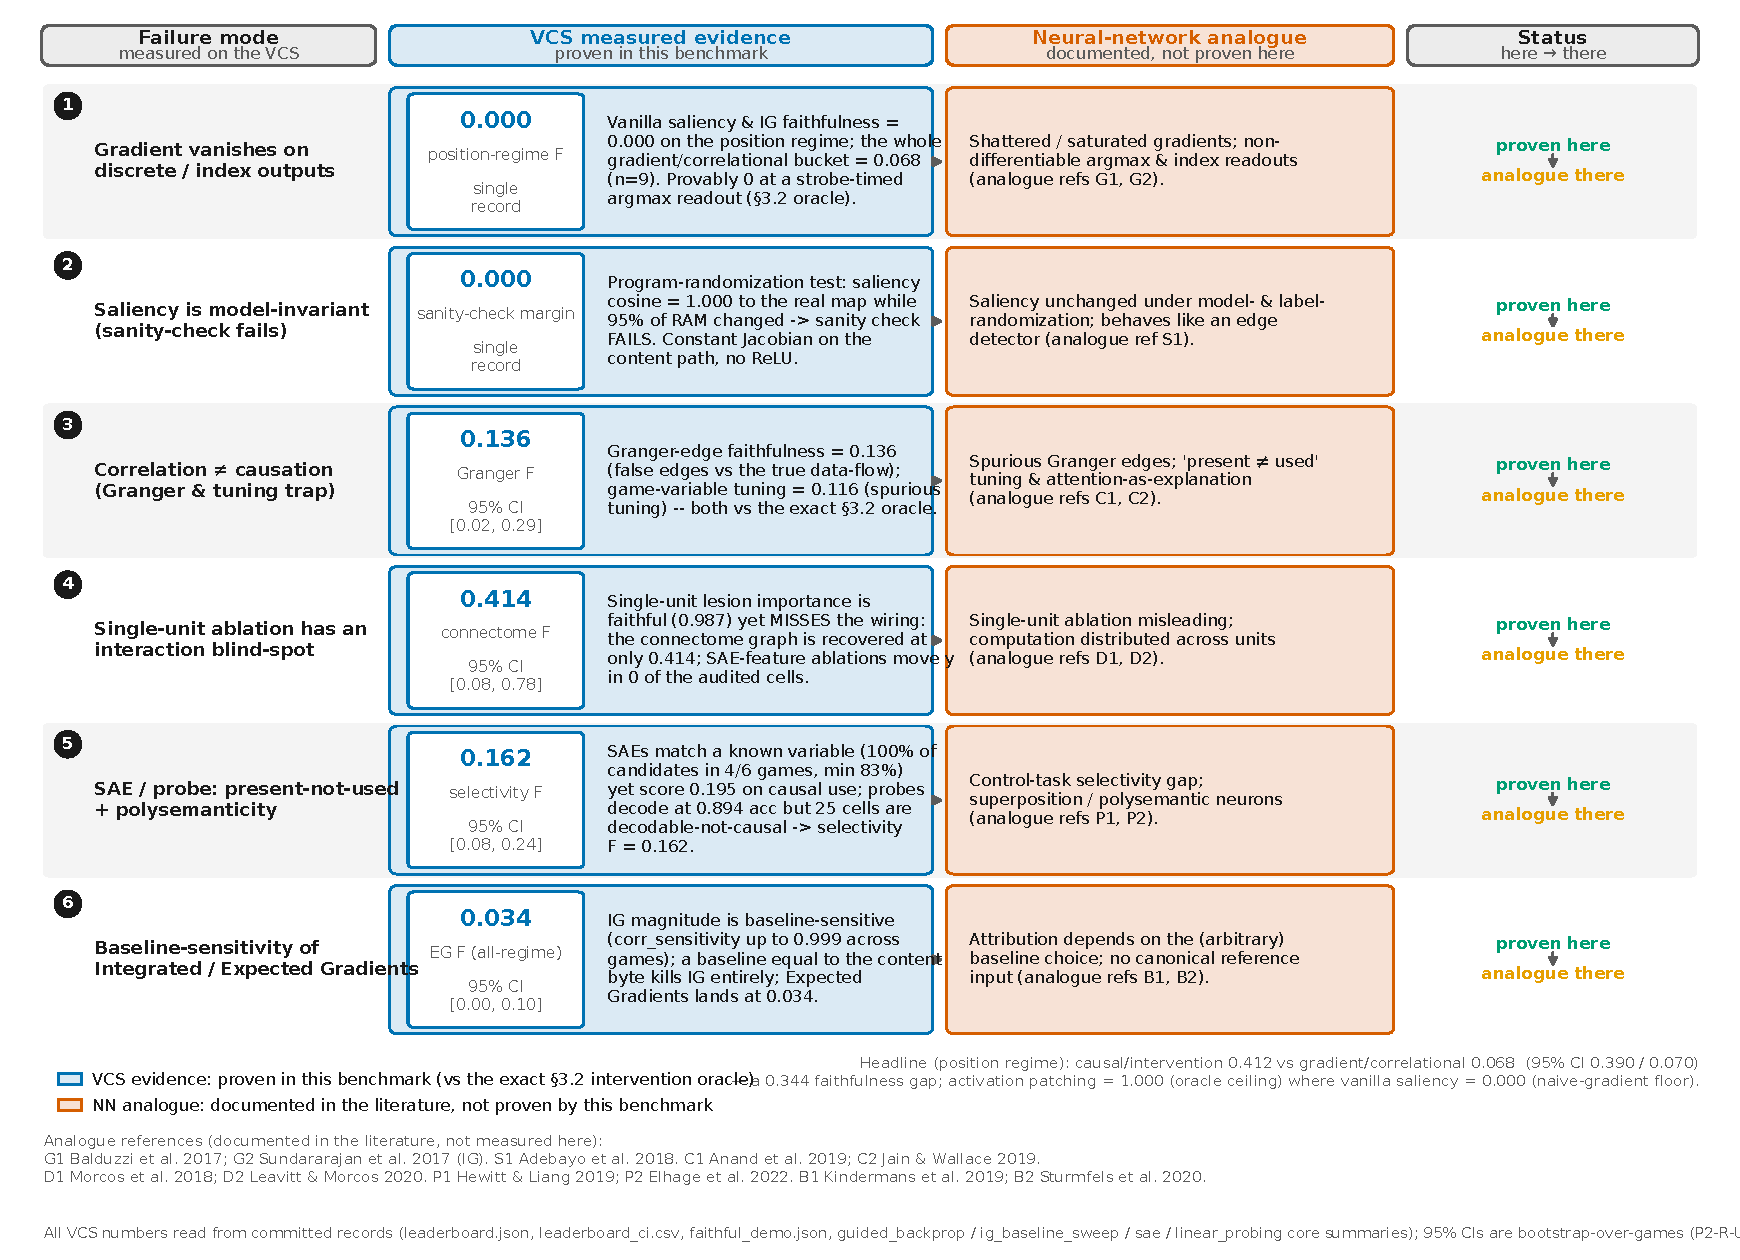
\includegraphics[width=\textwidth]{../figures/fig5_representativeness_map_full.pdf}
\caption{\textbf{Full VCS-to-NN representativeness map.} The full-density version of the
main-text map (Fig.~\ref{fig:representativeness}): each VCS failure mode is placed against its documented
neural-network analogue from the literature. The neural-network column records documented
analogues, not parallels proven by this benchmark; the oracle is the intervention oracle of
\Sectionname3.2, and the underlying per-method values trace to
\texttt{compare/out/leaderboard.json} via Sec.~\ref{supp:provenance}. Note that this full
map is the figure the simplified main-text version condenses.}
\label{supp:fig:repmap}
\end{figure}

\begin{figure}[t]
\centering
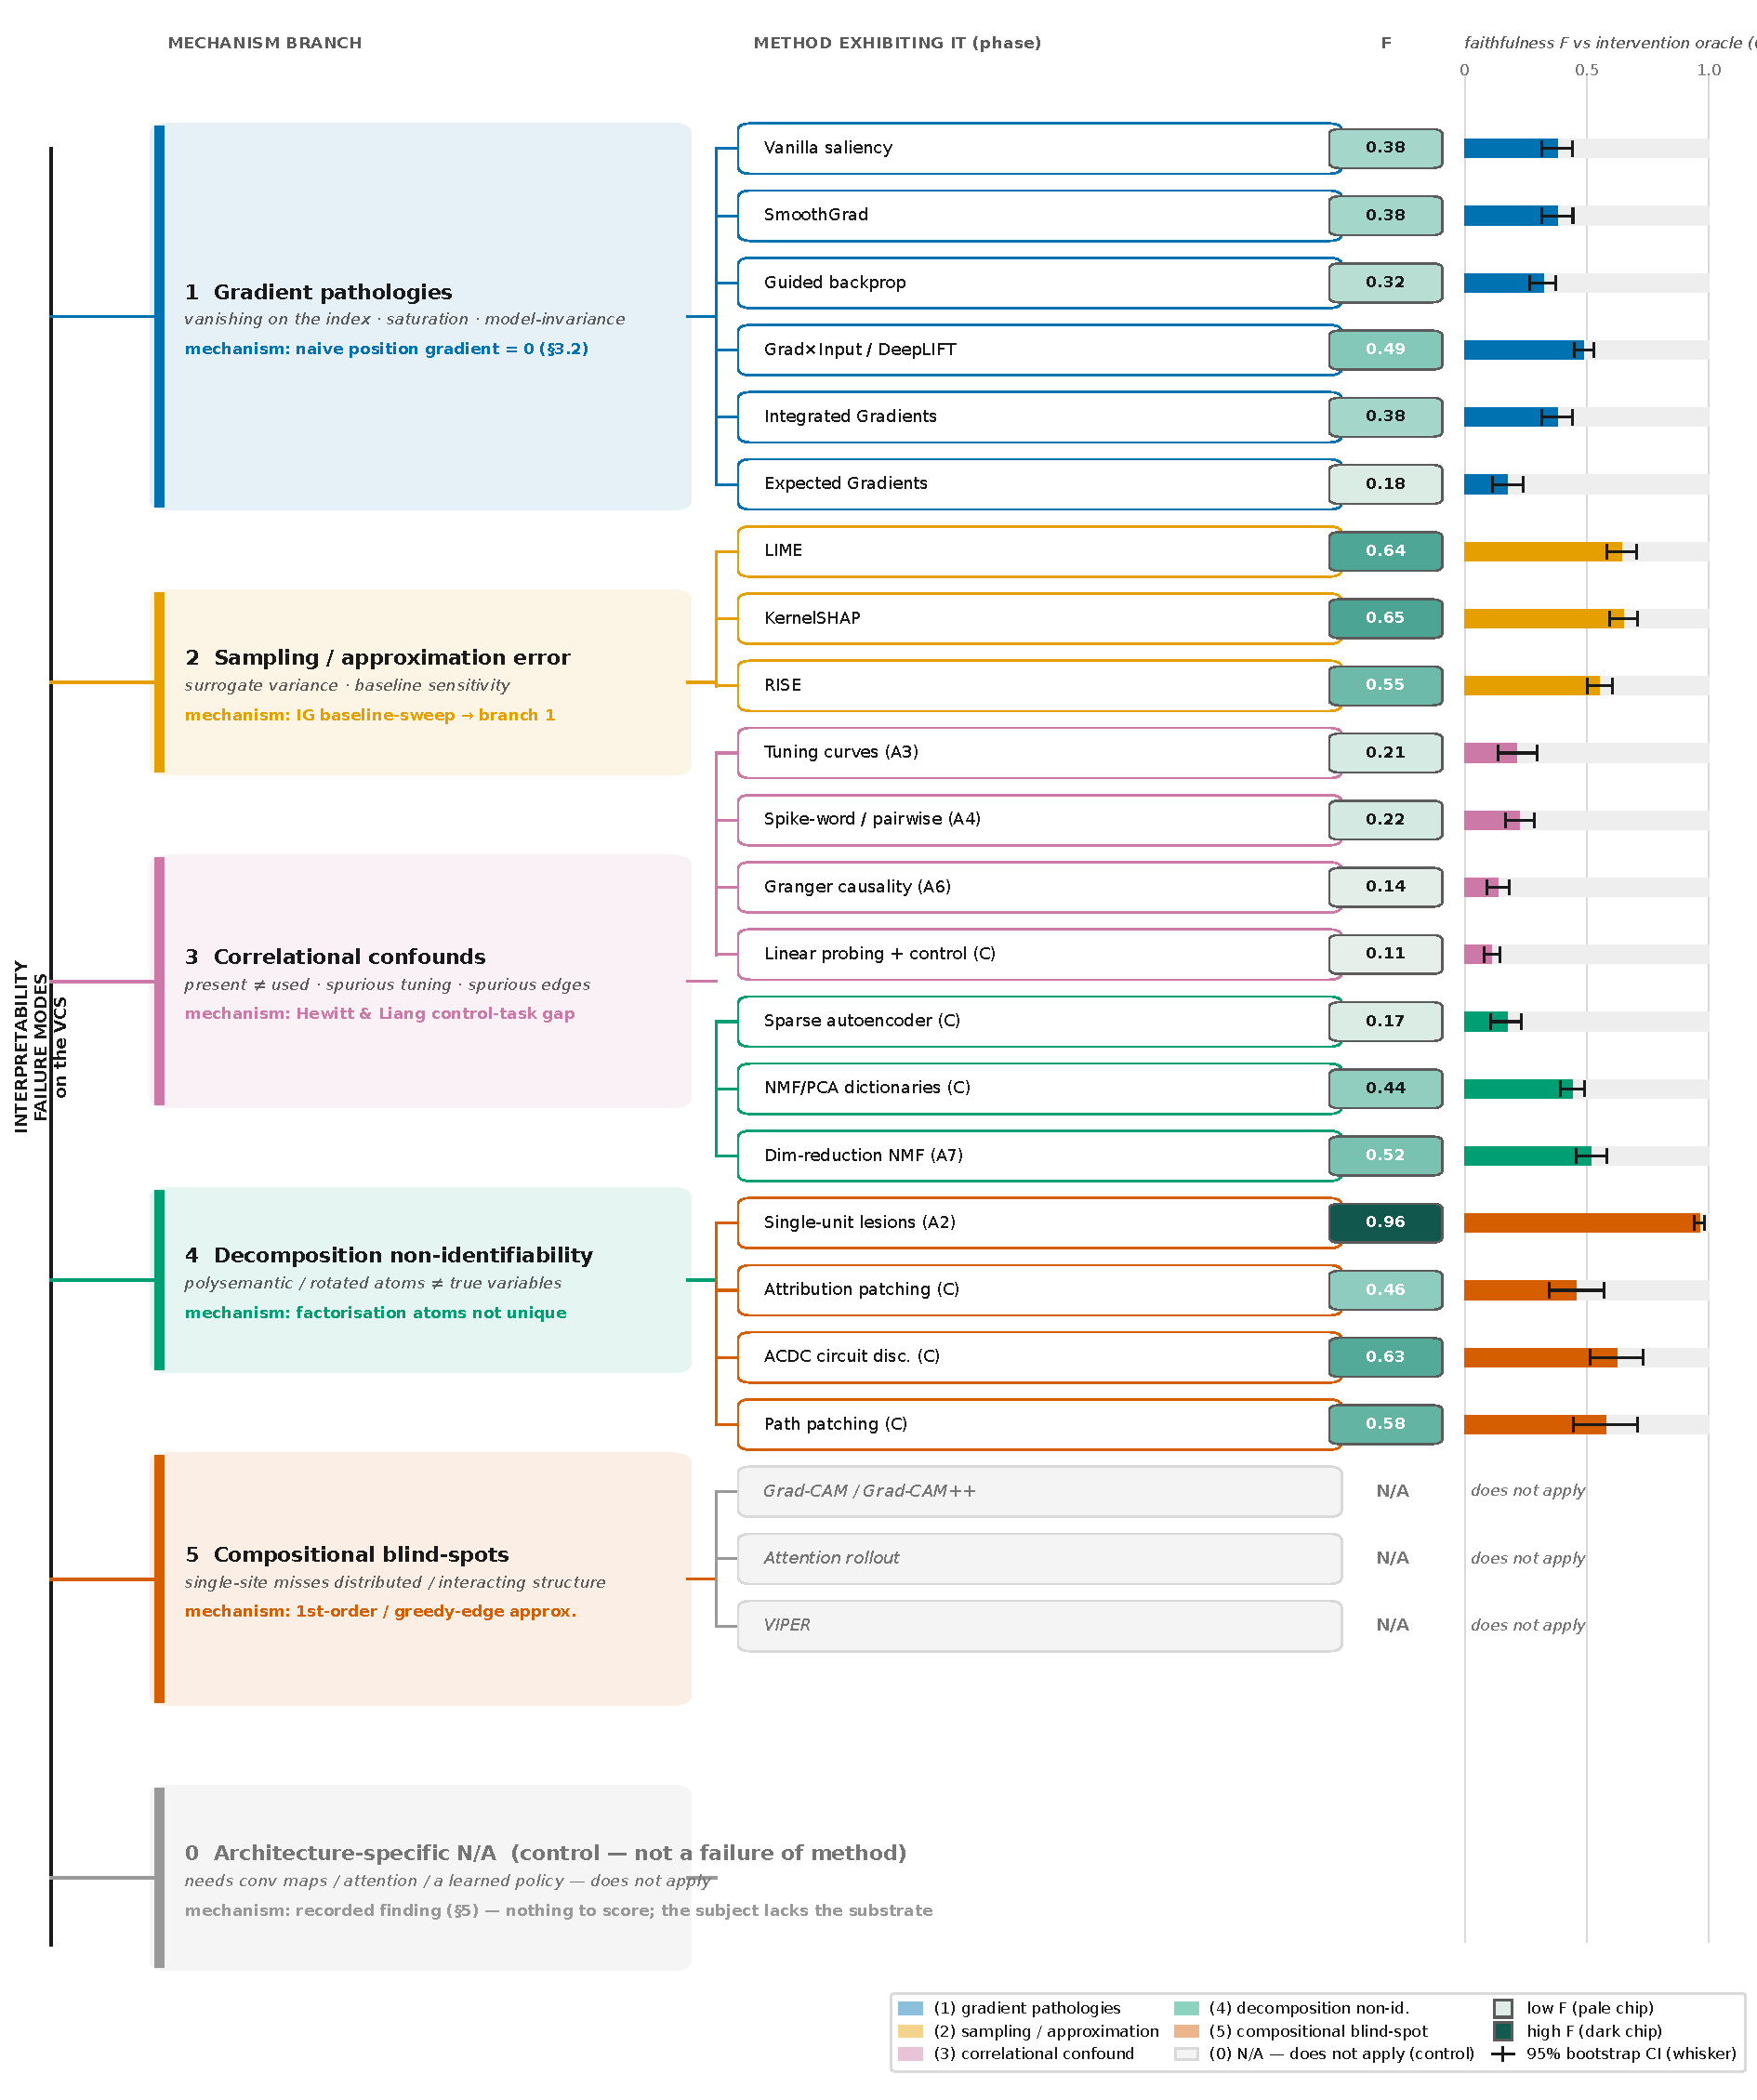
\includegraphics[width=\textwidth]{../figures/fig6_failure_taxonomy_full.pdf}
\caption{\textbf{Full failure taxonomy.} The full-density version of the main-text taxonomy
(Fig.~\ref{fig:taxonomy}): the families of interpretability failure observed on the machine, each annotated
with its faithfulness against the intervention oracle (\Sectionname3.2), reported as $F$ with its
$95\%$ bootstrap confidence interval. The leaf values trace to
\texttt{compare/out/leaderboard.json} and \texttt{leaderboard\_ci.csv} via
Sec.~\ref{supp:provenance}. Note that the gradient and correlational branches collapse on
the discrete position regime, where the naive gradient is provably zero (Prop.~\ref{prop:zero}).}
\label{supp:fig:taxonomy}
\end{figure}

\section{Plausibility-proxy rubric and its sensitivity}\label{supp:plausibility}

The plausibility axis of the leaderboard is a documented, tradition-level proxy, not a
human-subjects measurement. This section records how each value was assigned. It also shows
that the headline contrast does not depend on the particular numbers chosen. The Methods
(\Sectionname\ref{sec:triad}) name two reporting axes. Faithfulness is measured on the machine against the
intervention oracle of \Sectionname\ref{sec:oracle}. The plausibility proxy stands in for how convincing a
tradition's explanations are usually taken to be. We assign the proxy once per method
tradition, before any faithfulness score on our machine is computed, so it cannot be tuned to
the result. Its only job is to expose the danger zone of explanations that look convincing yet
are unfaithful. For that job it must be coarse, fixed in advance, and sourced rather than
precise.

The rubric assigns one proxy per tradition on a fixed five-step scale. It scores two
documented properties of each tradition's typical output and takes their average. The first
property is whether the explanation produces a dense, picture-like artifact that a reader sees
as an account of the computation. Heatmaps and saliency-style maps over the input are read as
convincing by construction. This is the perceptual-immediacy axis. The second property is
whether the field has historically treated the tradition's output as a self-evident
explanation rather than a hypothesis to be tested. This is the adoption-as-explanation axis. A
tradition that scores high on both, such as gradient saliency, receives a high proxy. A
tradition whose output is an austere intervention table or a circuit edge list, rarely
mistaken for a finished story, receives a low one. The scale is deliberately blunt,
$\{0.3,0.5,0.55,0.75,0.8,0.85,0.9\}$. A proxy meant to expose a danger zone gains nothing from
false precision, and a finer scale would invite over-reading. Every value in
Table~\ref{supp:tab:plausrubric} traces to the \jkey{plausibility_proxy} field of the
per-method rows in \texttt{compare/out/leaderboard.json}. The table only groups those rows by
tradition and records the rationale.

\begin{table}[t]
\centering
\caption{\textbf{Plausibility-proxy rubric.} The proxy assigned to each method tradition,
with the documented rationale. Values are the \jkey{plausibility_proxy} field of the
leaderboard rows (\texttt{compare/out/leaderboard.json}). They are tradition-level and fixed
before any faithfulness score is computed, so the proxy cannot be tuned to the measured
faithfulness. A higher value means an explanation that the field tends to find more
convincing, not one that is more faithful. The oracle (\Sectionname\ref{sec:oracle}) is the positive control and
is not a method under test.}
\label{supp:tab:plausrubric}
\begin{tabular}{@{}llp{6.4cm}@{}}
\toprule
Tradition & Proxy & Rationale (documented basis) \\
\midrule
gradient        & $0.90$ & Dense input-space heatmaps read as a visual account of the
                            decision; the most widely adopted XAI outputs, routinely shown
                            as if self-explanatory. \\
probing         & $0.85$ & A trained decoder that ``finds'' a concept reads as evidence the
                            concept is used; high adoption, though decodability is not
                            causal use. \\
correlational   & $0.80$ & Tuning curves and coupling spectra match the neuroscience idiom
                            of a convincing single-unit account. \\
dim.\ reduction & $0.75$ & Low-dimensional factors and dictionary atoms look like a clean
                            summary of the representation. \\
intervention    & $0.55$ & Occlusion and counterfactual outputs are quantitative tables, less
                            immediately picture-like, treated as tests rather than stories. \\
causal          & $0.50$ & Circuit edge lists and patching results are austere artifacts
                            rarely mistaken for a finished narrative. \\
descriptive     & $0.30$ & Whole-state recording is an explicit non-explanation: it withholds
                            nothing and reads as a dump, not an account. \\
\midrule
oracle (control)& $1.00$ & The \Sectionname\ref{sec:oracle} ground truth by construction; positive control, not a
                            method under test. \\
\bottomrule
\end{tabular}
\end{table}

The paper draws a contrast between this proxy and measured faithfulness. On the committed
records the two move in opposite directions. Across the thirty methods under test the Spearman
rank correlation between faithfulness and the proxy is $-0.36$, a negative association.
The traditions the field finds most convincing are, on this machine, among the least faithful.
Eight methods fall in the danger zone, defined here as a proxy of at least $0.70$ together
with a faithfulness below $0.40$. They include the correlational neuroscience methods, Expected
Gradients, guided backprop, linear probing, and the sparse autoencoder. The per-method extreme
makes the point sharply. Vanilla saliency has the highest proxy, $0.9$, yet scores faithfulness
$0.115$ on the position regime. Activation patching has a lower proxy, $0.5$, and scores $1.0$.
Here the less faithful method is the more plausible one. These figures are produced by
\texttt{tools/xai\_study/compare/plausibility\_sensitivity.py} from the leaderboard and
recorded in \texttt{compare/out/plausibility\_sensitivity.csv}.

A proxy fixed by a coarse rubric raises the question of whether the contrast is an artifact of
the particular numbers. The answer is that it is not. We perturb the proxy under four
deterministic schemes and recompute the relationship each time. The analysis uses fixed,
index-keyed offsets rather than random draws, so it re-derives bit-for-bit. The first scheme
adds a fixed per-method jitter of magnitude $\sigma\in\{0.05,0.1,0.2\}$, alternating in sign by
row. The second compresses every proxy toward the common mean by a fraction $\sigma$, which
preserves the rank order of traditions. The third uses the same index-keyed offsets at
$\sigma\in\{0.1,0.2\}$, large enough to swap neighbouring traditions' ranks. The fourth drops
one whole tradition at a time and recomputes on the remainder. Across all fourteen
perturbations the rank correlation between faithfulness and proxy stays negative. It ranges
from $-0.76$ to $-0.08$. The danger zone stays populated, with
between four and ten methods. The per-method anchor sign holds in every scheme where both
anchor methods are present, the more plausible saliency remaining the less faithful. Two runs
bound the range. The strongest is the leave-the-gradient-tradition-out run. It removes the most
plausible and least faithful block at once, and still leaves six danger-zone methods and a rank
correlation of $-0.76$. The weakest is the leave-the-causal-tradition-out run, where the
correlation falls to $-0.08$, close to zero; removing the faithful causal block flattens the
association, so the contrast is carried in part by that block. Table~\ref{supp:tab:plaussens}
reports the full sweep. The contrast keeps its sign under every alternative proxy assignment we
tried: plausibility and faithfulness are not the same axis, and high plausibility is no
guarantee of faithfulness.

\begin{table}[t]
\centering
\caption{\textbf{Proxy-sensitivity sweep.} The faithfulness-versus-proxy relationship under
each perturbation, from \texttt{compare/out/plausibility\_sensitivity.csv}. ``$\rho$'' is the
Spearman rank correlation between faithfulness and proxy over the methods present. ``danger''
is the count of high-proxy ($\geq0.70$), low-faithfulness ($<0.40$) methods. ``anchor'' is
$1$ when the more plausible saliency is the less faithful of the saliency/activation-patching
pair, and blank where a leave-one-out run removes an anchor. The baseline rubric is the first
row. Across every scheme the correlation stays negative and the danger zone stays populated.}
\label{supp:tab:plaussens}
\begin{tabular}{@{}llrrrc@{}}
\toprule
Scheme & Param & $n$ & $\rho$ & Danger & Anchor \\
\midrule
baseline                & ---           & 30 & $-0.36$ &  8 & 1 \\
additive jitter         & $\sigma=0.05$ & 30 & $-0.40$ &  8 & 1 \\
additive jitter         & $\sigma=0.10$ & 30 & $-0.41$ &  8 & 1 \\
additive jitter         & $\sigma=0.20$ & 30 & $-0.42$ & 10 & 1 \\
rank-preserving         & $\sigma=0.10$ & 30 & $-0.36$ &  8 & 1 \\
rank-preserving         & $\sigma=0.20$ & 30 & $-0.36$ &  8 & 1 \\
rank-jittering          & $\sigma=0.10$ & 30 & $-0.41$ &  8 & 1 \\
rank-jittering          & $\sigma=0.20$ & 30 & $-0.42$ & 10 & 1 \\
leave-out causal        & ---           & 24 & $-0.08$ &  8 & \\
leave-out correlational & ---           & 26 & $-0.40$ &  4 & 1 \\
leave-out descriptive   & ---           & 29 & $-0.29$ &  8 & 1 \\
leave-out dim.\ red.    & ---           & 27 & $-0.34$ &  7 & 1 \\
leave-out gradient      & ---           & 20 & $-0.76$ &  6 & \\
leave-out intervention  & ---           & 25 & $-0.34$ &  8 & 1 \\
leave-out probing       & ---           & 29 & $-0.36$ &  7 & 1 \\
\bottomrule
\end{tabular}
\end{table}

